%% -----------------------------------------------------------------------------
%% Tiago Fonseca - Doctoral Thesis
%% Main document for Overleaf and local compilation.
%% -----------------------------------------------------------------------------

\documentclass[11pt,a4paper,twoside,openright]{report}

% FEUP generic thesis format. The generic option is used for PhD programmes.
% Working version:
\usepackage{feupteses}
% Jury version:
% \usepackage[juri]{feupteses}
% Final electronic version:
% \usepackage[final]{feupteses}
% Printed final version:
% \usepackage[final,onpaper]{feupteses}

\graphicspath{{figures/}}

% Mathematics, diagrams, cross-references, and thesis utilities.
\usepackage{amsmath,amssymb,mathtools}
\usepackage{bm}
\usepackage{tikz}
\usetikzlibrary{arrows.meta,positioning,fit,shapes.geometric}
\usepackage[capitalise,noabbrev]{cleveref}
\usepackage{pifont}
\usepackage{ragged2e}
\usepackage{tabularx}
\usepackage{comment}

% Bibliography. Biber is selected automatically by Overleaf when required.
\usepackage[
  backend=biber,
  style=authoryear-comp,
  maxcitenames=2,
  maxbibnames=99,
  uniquename=false,
  giveninits=true,
  doi=true,
  url=true,
  isbn=false
]{biblatex}
\addbibresource{bibliography/references.bib}

% Acronyms and glossary without an external indexing step.
\usepackage[acronym,toc,nonumberlist]{glossaries-extra}
\makenoidxglossaries
% Acronyms --------------------------------------------------------------------
\newacronym{ai}{AI}{Artificial Intelligence}
\newacronym{api}{API}{Application Programming Interface}
\newacronym{ac}{AC}{Alternating Current}
\newacronym{boptest}{BOPTEST}{Building Optimization Testing Framework}
\newacronym{cpu}{CPU}{Central Processing Unit}
\newacronym{csv}{CSV}{Comma-Separated Values}
\newacronym{dc}{DC}{Direct Current}
\newacronym{fmi}{FMI}{Functional Mock-up Interface}
\newacronym{g2v}{G2V}{Grid-to-Vehicle}
\newacronym{gpu}{GPU}{Graphics Processing Unit}
\newacronym{helics}{HELICS}{Hierarchical Engine for Large-scale Infrastructure Co-Simulation}
\newacronym{hpc}{HPC}{High-Performance Computing}
\newacronym{lstm}{LSTM}{Long Short-Term Memory}
\newacronym{mappo}{MAPPO}{Multi-Agent Proximal Policy Optimization}
\newacronym{onnx}{ONNX}{Open Neural Network Exchange}
\newacronym{cps}{CPS}{Cyber-Physical System}
\newacronym{ctde}{CTDE}{Centralised Training with Decentralised Execution}
\newacronym{der}{DER}{Distributed Energy Resource}
\newacronym{decpomdp}{Dec-POMDP}{Decentralised Partially Observable Markov Decision Process}
\newacronym{dr}{DR}{Demand Response}
\newacronym{ems}{EMS}{Energy Management System}
\newacronym{ev}{EV}{Electric Vehicle}
\newacronym{evse}{EVSE}{Electric Vehicle Supply Equipment}
\newacronym{hil}{HIL}{Hardware-in-the-Loop}
\newacronym{gdpr}{GDPR}{General Data Protection Regulation}
\newacronym{hvac}{HVAC}{Heating, Ventilation, and Air Conditioning}
\newacronym{iot}{IoT}{Internet of Things}
\newacronym{kpi}{KPI}{Key Performance Indicator}
\newacronym{maddpg}{MADDPG}{Multi-Agent Deep Deterministic Policy Gradient}
\newacronym{madrl}{MADRL}{Multi-Agent Deep Reinforcement Learning}
\newacronym{marl}{MARL}{Multi-Agent Reinforcement Learning}
\newacronym{mas}{MAS}{Multi-Agent System}
\newacronym{mdp}{MDP}{Markov Decision Process}
\newacronym{ml}{ML}{Machine Learning}
\newacronym{mlops}{MLOps}{Machine Learning Operations}
\newacronym{mpc}{MPC}{Model Predictive Control}
\newacronym{ocpp}{OCPP}{Open Charge Point Protocol}
\newacronym{opeva}{OPEVA}{Optimisation of Electric Vehicle Autonomy}
\newacronym{pomdp}{POMDP}{Partially Observable Markov Decision Process}
\newacronym{pv}{PV}{Photovoltaic}
\newacronym{rbc}{RBC}{Rule-Based Controller}
\newacronym{rec}{REC}{Renewable Energy Community}
\newacronym{rest}{REST}{Representational State Transfer}
\newacronym{rl}{RL}{Reinforcement Learning}
\newacronym{rlops}{RLOps}{Reinforcement Learning Operations}
\newacronym{rq}{RQ}{Research Question}
\newacronym{soc}{SoC}{State of Charge}
\newacronym{tou}{ToU}{Time of Use}
\newacronym{v2g}{V2G}{Vehicle-to-Grid}
\newacronym{bc}{BC}{Behaviour Cloning}
\newacronym{bess}{BESS}{Battery Energy Storage System}
\newacronym{gnn}{GNN}{Graph Neural Network}
\newacronym{hrl}{HRL}{Hierarchical Reinforcement Learning}
\newacronym{matd3}{MATD3}{Multi-Agent Twin Delayed Deep Deterministic Policy Gradient}
\newacronym{milp}{MILP}{Mixed-Integer Linear Programming}
\newacronym{ood}{OOD}{Out of Distribution}
\newacronym{per}{PER}{Prioritized Experience Replay}
\newacronym{ppo}{PPO}{Proximal Policy Optimization}
\newacronym{sac}{SAC}{Soft Actor-Critic}
\newacronym{td3}{TD3}{Twin Delayed Deep Deterministic Policy Gradient}
\newacronym{timdp}{TI-MDP}{Typed-Interface Markov Decision Process}
\newacronym{tirl}{TI-RL}{Typed-Interface Reinforcement Learning}
\newacronym{timg}{TIMG}{Typed-Interface Markov Game}
\newacronym{timarl}{TI-MARL}{Typed-Interface Multi-Agent Reinforcement Learning}
\newacronym{tic}{TIC}{Typed Interface Compiler}
\newacronym{tip}{TIP}{Typed-Interface Policy}
\newacronym{tcg}{TCG}{Typed Constraint Graph}
\newacronym{ral}{RAL}{Runtime Assurance Layer}
\newacronym{vpp}{VPP}{Virtual Power Plant}

% Glossary terms ----------------------------------------------------------------
\newglossaryentry{agent}{
  name={agent},
  description={A decision-making entity that receives observations, selects actions, and pursues one or more objectives within an environment. In this thesis, an agent may represent a participant, building, charging installation, or controllable resource, depending on the control setting}
}

\newglossaryentry{asset}{
  name={energy asset},
  description={A physical or virtual energy resource that can be observed or controlled, such as an electric vehicle, charger, battery, photovoltaic system, heat pump, or flexible electrical load}
}

\newglossaryentry{policy}{
  name={policy},
  description={A mapping from the information available to an agent to the action selected by that agent. A policy may be rule-based, optimisation-based, or learned}
}

\newglossaryentry{controller}{
  name={controller},
  description={The software or physical component responsible for producing control actions. A controller may implement a rule-based strategy, an optimisation method, or a learned policy}
}

\newglossaryentry{community}{
  name={community},
  description={A set of participants and energy assets coordinated under shared rules or objectives. In the principal case studies, this term refers to a renewable energy community}
}

\newglossaryentry{dynamicreconfiguration}{
  name={dynamic reconfiguration},
  description={A change in the composition, availability, capabilities, or interaction structure of a system during or between operating periods, such as an electric vehicle arriving or leaving, an asset becoming unavailable, or a new participant joining a community}
}

\newglossaryentry{scalability}{
  name={scalability},
  description={The ability of an algorithm, simulator, infrastructure, or deployed system to accommodate increasing numbers of agents, assets, interactions, experiments, or devices without unacceptable loss of performance or excessive resource use}
}

\newglossaryentry{deployability}{
  name={deployability},
  description={The ability to package, validate, install, configure, execute, monitor, update, and recover a control solution or coordinated policy set within its intended operational environment}
}


\newglossaryentry{policyset}{
  name={policy set},
  description={A governed collection of interdependent policies intended to operate together, including their agent-role mappings, observation and action schemas, communication assumptions, safety dependencies, compatibility rules, and shared deployment version}
}

\newglossaryentry{policyregistry}{
  name={policy registry},
  description={A lifecycle service that records policy identity, versions, provenance, evaluation evidence, compatibility metadata, promotion state, deployment associations, and rollback lineage, rather than storing only model bytes}
}

\newglossaryentry{experimentmanifest}{
  name={experiment manifest},
  description={An immutable or content-addressed record that links an experiment to its source revision, environment, scenario and data, reward, observations and actions, constraints, seeds, algorithm configuration, dependencies, resources, and resulting artefacts}
}

\newglossaryentry{coordinationmonitoring}{
  name={coordination-aware monitoring},
  description={Operational monitoring that detects failures in the relationships among agents and policies, such as incompatible versions, oscillating or conflicting actions, stale messages, unfair shared-resource allocation, or degradation of a community-level objective despite healthy processes}
}

\newglossaryentry{safety}{
  name={safety},
  description={The prevention of unacceptable actions or system states through the satisfaction of physical, operational, and user-related constraints}
}

\newglossaryentry{robustness}{
  name={robustness},
  description={The ability to maintain acceptable behaviour and performance under uncertainty, disturbances, faults, imperfect data, dynamic reconfiguration, or differences between training and operation}
}

\newglossaryentry{resilience}{
  name={resilience},
  description={The ability of a system to recover after a fault, disruption, or period of degraded operation}
}

\newglossaryentry{transferability}{
  name={transferability},
  description={The extent to which knowledge, representations, or policies learned in one setting can be reused or adapted in a different agent, configuration, scenario, or environment}
}

\newglossaryentry{realworld}{
  name={real-world operation},
  description={Execution under physical, computational, communication, organisational, and lifecycle constraints that are not fully represented by a conventional isolated simulation experiment}
}

\newglossaryentry{energAIze}{
  name={EnergAIze},
  description={The integrated research platform and energy-domain reference implementation through which the methods, software components, lifecycle mechanisms, and demonstrators developed in this thesis are connected and evaluated}
}


\newglossaryentry{entity}{
  name={entity},
  description={A runtime object that gives observations or actions a concrete identity and operational meaning, such as a connected electric-vehicle session, charger, battery, or other controlled or observed object within an agent}
}

\newglossaryentry{moduleinstance}{
  name={module instance},
  description={A concrete runtime instance of a capability-bearing component associated with an agent, such as one charger, battery, or controllable subsystem; module instances may appear, disappear, or change availability without redefining the complete policy architecture}
}

\newglossaryentry{capabilityschema}{
  name={capability schema},
  description={A versioned description of the potential observations, action groups, action ports, constraints, compatibility requirements, and fallback semantics that an agent or module type can expose}
}

\newglossaryentry{runtimehealth}{
  name={runtime health state},
  description={The current quality and availability state of observations, modules, communication channels, or controlled entities used by the Typed Interface Compiler to determine validity, bounds, degraded modes, and fallback behaviour}
}

\newglossaryentry{actiongroup}{
  name={action group},
  description={A set of mutually exclusive action ports representing alternative operating modes for one controllable function or entity, while compatible action groups may be controlled simultaneously within the same local action bundle}
}

\newglossaryentry{compatibilitysignature}{
  name={compatibility signature},
  description={A versioned summary of interface and capability requirements used to determine whether a policy, compiler, schema, and runtime target can operate together safely}
}

\newglossaryentry{localfeasibility}{
  name={local feasibility},
  description={The construction or adjustment of an agent's local action bundle so that simultaneous actions remain within non-negotiable local physical, device, and service constraints while preserving policy intent as far as possible}
}

\newglossaryentry{sharedhardmonitor}{
  name={shared hard-constraint monitor},
  description={An exceptional runtime assurance mechanism that detects and, when necessary, minimally corrects or rejects joint actions that would violate non-negotiable constraints shared across agents; it is not the normal community optimisation mechanism}
}

\newglossaryentry{typedinterface}{
  name={typed interface},
  description={A runtime contract that describes an agent's available observation parts, action ports, parameter types and bounds, validity conditions, capabilities, and constraints rather than assuming one permanently fixed flat observation and action vector}
}

\newglossaryentry{observationpart}{
  name={observation part},
  description={A typed block of information exposed to a policy, such as self state, scanner status, battery state of charge, deadline, entity relation, or measurement-quality indicator}
}

\newglossaryentry{actionport}{
  name={action port},
  description={A callable typed action exposed by the current agent interface, including its semantic name, parameters, bounds, validity conditions, and any projection or safety rule applied before execution}
}

\newglossaryentry{failsafemode}{
  name={fail-safe mode},
  description={A controlled operating state in which a learned controller is constrained, bypassed, or replaced by a conservative controller because data, communication, policy compatibility, confidence, or safety conditions are not sufficient for normal operation}
}


\newglossaryentry{behaviourcloning}{
  name={behaviour cloning},
  description={Supervised policy learning from state--action demonstrations produced by an expert, rule-based controller, optimiser, or previously deployed policy}
}

\newglossaryentry{offlinerl}{
  name={offline reinforcement learning},
  description={Reinforcement learning from a fixed dataset of previously collected transitions or trajectories without additional environment interaction during the offline training stage}
}

\newglossaryentry{physicsinformedrl}{
  name={physics-informed reinforcement learning},
  description={A family of approaches that incorporates physical models, invariants, residuals, constraints, or model-based structure into policy learning, value estimation, action validation, or training objectives}
}


\newglossaryentry{actionbundleintent}{
  name={local action bundle},
  description={The structured action produced by one local typed-interface policy, containing one selected port and its parameters for each active action-group instance after local hard-feasibility construction}
}

\newglossaryentry{actiongroupinstance}{
  name={action-group instance},
  description={A runtime controllable group bound to a specific module or entity instance, such as the operating mode of one particular EV charger; the same shared decoder can be applied to multiple instances of the same group type}
}

\newglossaryentry{entityboundinterface}{
  name={entity-bound typed interface},
  description={A runtime observation--action interface in which observation parts, action groups, and ports explicitly identify the module and controlled entity that give them meaning}
}

\newglossaryentry{healthclosure}{
  name={health closure},
  description={The deterministic propagation of source or module health through declared dependencies to observation validity, action-port availability, parameter bounds, action groups, constraints, and operational mode}
}

\newglossaryentry{typeddecisiontrace}{
  name={typed decision trace},
  description={An execution record grounded in the actual interface snapshot, including active entities, observations and health, available and invalid ports, selected actions, local feasibility adjustments, shared safety interventions, and final commands}
}

\newglossaryentry{interfacesnapshot}{
  name={interface snapshot},
  description={An immutable record of the observation parts, action ports, dependencies, validity states, bounds, health, and resource couplings exposed to an agent at one decision step}
}

\newglossaryentry{typedconstraintgraph}{
  name={typed constraint graph},
  description={A runtime graph connecting agents, modules, entities, action ports, resources, topology, and local or shared constraints through typed relations; it supports local bundle feasibility, training-time graph critics, hard shared checks, compatibility, and decision traces}
}


% -----------------------------------------------------------------------------
% Central metadata. Edit this file instead of searching throughout the project.
% -----------------------------------------------------------------------------

\newcommand{\ThesisAuthor}{Tiago Carlos Caló Fonseca}
\newcommand{\ThesisTitle}{Multi-Agent Reinforcement Learning Control of Renewable Energy Communities}
\newcommand{\ThesisDegree}{Programa Doutoral em Engenharia Informática}
\newcommand{\ThesisDate}{December 2026}
\newcommand{\ThesisSupervisor}{Luís Miguel Moreira Lino Ferreira, PhD}
\newcommand{\ThesisCoSupervisor}{Armando Jorge Sousa, PhD}

\renewcommand{\preprologpages}{%
  \cleardoublepage
  \thispagestyle{empty}
\vspace*{0.34\textheight}
\begin{center}
{\Large\itshape ``For the things we have to learn before we can do them, we learn by doing them.''\par}
\vspace{12mm}
{\large Aristotle\par}
\vspace{2mm}
{\small\itshape Nicomachean Ethics\par}
\end{center}
\vfill
\clearpage
%
  \thispagestyle{empty}
\vspace*{\fill}
\begin{center}
\copyright\ \ThesisAuthor, 2026
\end{center}
\clearpage
%
}

\title{\ThesisTitle}
\author{\ThesisAuthor}
\degree{\ThesisDegree}
\thesisdate{\ThesisDate}
% Keep the review cover visually identical to the final cover without enabling
% the jury/committee pages before their metadata has been confirmed.
\additionalfronttext{}
% The title verso is blank; the epigraph opens on the next recto.
% Copyright occupies the epigraph verso before the numbered front matter.
\logo{uporto-feup}

\supervisor{Supervisor}{\ThesisSupervisor}
\supervisor{Co-Supervisor}{\ThesisCoSupervisor}

% Committee details are intentionally left commented in the working version.
% Uncomment and complete when preparing the jury or final version.
% \committeetext{Approved in oral examination by the committee:}
% \committeemember{President}{Prof. [Name]}
% \committeemember{Referee}{Prof. [Name]}
% \committeemember{Referee}{Prof. [Name]}

\hypersetup{
  pdftitle={\ThesisTitle},
  pdfauthor={\ThesisAuthor},
  pdfsubject={Doctoral thesis in Informatics Engineering},
  pdfkeywords={multi-agent reinforcement learning, cyber-physical systems, renewable energy communities, scalability, deployability, safety, robustness},
  pdfstartpage={1},
  pdfstartview={FitH},
  pdfpagemode={UseNone}
}


\begin{document}

\begin{Prolog}
  \frontmatterchapter{Declaration of Honour}

I hereby declare on my honour that this thesis (or dissertation) is my own original work and that all sources used have been acknowledged and properly cited. I am aware that the use of unauthorized third-party text, data, or figures constitutes plagiarism and is a serious breach of academic integrity.

\vspace{18mm}
\noindent Porto, \rule{16mm}{0.4pt} of \rule{42mm}{0.4pt} of 20\rule{10mm}{0.4pt}

\vspace{20mm}
\begin{center}
  \rule{0.72\linewidth}{0.4pt}\\
  \emph{(Signature of the Student)}
\end{center}

  \frontmatterchapter{Declaration on the Use of Generative Artificial Intelligence}

Generative Artificial Intelligence was used as a supporting tool during the preparation of this thesis, including for research organisation, drafting, language revision, and software-related assistance.

All material included in the thesis was critically reviewed, verified, rewritten where necessary, and integrated by the author. The author remains fully responsible for the research design, source selection, software, experiments, data analysis, interpretation of results, scientific arguments, and final text.

  \frontmatterchapter{Statement on Co-Authored Work}

The research presented in this thesis was conducted within an integrated project whose overall architecture was conceived and defined by the author. This architecture provided a common conceptual and technical framework for the supporting components described throughout the thesis. Several of these components were developed collaboratively with supervisors, research colleagues, students, open-source contributors, and industrial partners. The corresponding lines of work were proposed and formulated by the author, who also contributed to their technical direction, development, supervision, validation, and integration.

As the nature and extent of the collaboration varied between components, the following table records the persons involved, the author's specific contribution, and the location of each component within the thesis. Publications arising from this work are reported separately in the list of research outputs and in the references.

\vspace{6mm}

\begingroup
\renewcommand{\arraystretch}{1.35}
\small
\begin{tabularx}{\textwidth}{@{}p{0.22\textwidth}p{0.20\textwidth}Xp{0.15\textwidth}@{}}
\hline
\textbf{Component or tool} & \textbf{Co-author(s) or contributor(s)} & \textbf{Author's contribution} & \textbf{Thesis location} \\
\hline
\textit{[Title or name]} & \textit{[Name(s)]} & \textit{[Concise contribution]} & \textit{[Ch./Sec.]} \\
\textit{[Title or name]} & \textit{[Name(s)]} & \textit{[Concise contribution]} & \textit{[Ch./Sec.]} \\
\textit{[Title or name]} & \textit{[Name(s)]} & \textit{[Concise contribution]} & \textit{[Ch./Sec.]} \\
\textit{[Title or name]} & \textit{[Name(s)]} & \textit{[Concise contribution]} & \textit{[Ch./Sec.]} \\
\hline
\end{tabularx}
\endgroup

\vspace{3mm}
The author retains responsibility for the selection, verification, integration, and interpretation of these components as presented in the thesis. Additional contributions are acknowledged in the relevant sections and do not alter the author's responsibility for the scientific arguments and conclusions reported herein.

  % \cleardoublepage
\thispagestyle{empty}
\vspace*{0.35\textheight}
\begin{flushright}
\emph{[Optional dedication]}
\end{flushright}
\clearpage

  \frontmatterchapter{Acknowledgements}

Sincere thanks go to the supervisor, Luís Miguel Moreira Lino Ferreira, PhD, and the co-supervisor, Armando Jorge Sousa, PhD, for their guidance and trust. Throughout many meetings, they made time to listen to my ideas, discuss different possibilities, and return to questions as the research developed. These conversations helped shape the work and were among the most meaningful parts of the doctoral experience.

Particular thanks are due to the industrial partners CleanWatts, especially Eng.~Jorge Landeck, and i-Charging, especially Eng.~Paulo Rodrigues. Their experience with energy systems and electric-vehicle charging brought a practical understanding of the constraints encountered during the work in OPEVA.

The students whose theses and research projects developed alongside this work made supervision a source of learning. Their questions opened up different ways of approaching related problems, and the opportunity to accompany their projects from an initial idea through development and validation was especially valuable.

\draftnote{Add the names of the students the author wishes to thank individually.}

Friends and colleagues at FEUP made the day-to-day experience of the doctorate easier to share. João Vitorino and Tiago Dias deserve a special mention for the conversations, shared frustrations, and laughter that accompanied these years.

My parents, Vera and Abílio, deserve a particularly warm word of thanks. They provided the stability and opportunities on which this path was built, long before the doctorate began. Their encouragement sustained choices that sometimes demanded patience and sacrifice from them, and their example taught the value of work, responsibility, and perseverance. The affection and presence of my grandparents were equally important, giving a sense of family that extended far beyond the years devoted to this thesis.

The final and most personal thanks go to Inês. She shared the achievements of the doctorate and lived closely with the pressure and exhaustion it brought into everyday life. There were periods when the work took up too much space, and its frustrations followed it home as impatience, distraction, or withdrawal. Her support continued through those periods, even when it was difficult to give. She made time to listen and helped restore perspective when a research problem seemed to occupy everything. She celebrated progress that was too easily dismissed, offered encouragement when confidence faltered, and knew when a challenge would help more than reassurance. Her belief remained steady through long periods of doubt and slow progress. The patience and affection behind that support meant a great deal to the completion of this work and to the shared life that continued around it. The order of a finished thesis conceals much of the uncertainty and repetition involved in writing it. Inês accompanied that less orderly part of the work too, with a patience and affection for which these pages offer only a small acknowledgement.

Nes, Pai, Mae, Aida, Vo Ek e Vo Fonso.

  \frontmatterchapter{Abstract}

Cyber-physical systems increasingly rely on distributed autonomous control while operating under heterogeneous capabilities, changing configurations, incomplete information, communication limitations, and physical constraints. Multi-Agent Reinforcement Learning (MARL) provides a promising basis for such control, but good performance in simulation does not by itself establish that a learned policy can be used reliably in an operational system. This thesis addresses that transition through four connected requirements: scalability, deployability, safety, and robustness. Renewable Energy Communities and electric-vehicle charging provide the principal empirical domain, combining distributed participants, heterogeneous flexible assets, changing availability, local and collective objectives, and shared physical infrastructure.

The research develops EnergAIze as an integrated architecture for the development and operation of intelligent energy control. It connects data and scenario construction, an extended CityLearn-derived simulation environment, controller development, reproducible experimentation, policy governance, distributed deployment, monitoring, and recovery. Within this architecture, a progression of rule-based, optimisation-based, reinforcement-learning, and multi-agent methods establishes increasingly capable control solutions and provides empirical evidence about the assumptions under which each remains effective.

These findings motivate TI-MARL, the principal algorithmic contribution of the thesis. TI-MARL addresses multi-agent decision problems in which the observation--action interface of an agent can change during operation. A versioned capability schema and runtime health information are compiled into an entity-bound typed interface containing the observation parts, action-group instances, parameterised action ports, dependencies, validity conditions, and bounds currently available to the agent. A decentralised policy operates directly over this variable interface, constructs a shared local representation, and jointly produces a coherent action bundle for the controllable entities that are present. Local hard constraints are incorporated into action construction, while coordination between agents is learned through authorised shared observations, coupled objectives, the joint physical transition, and centralised variable-population critics during training.

The resulting methods and infrastructure are evaluated through simulator verification, common controller comparisons, dynamic reconfiguration, health and disturbance tests, ablations, multi-dimensional scalability experiments, lifecycle and compatibility tests, edge execution, and integrated energy scenarios. Selected components are further assessed using real data, external energy platforms, charging infrastructure, edge services, and physical demonstrators, with the evidence level distinguished explicitly from simulation to direct operational control. Taken together, the thesis shows how algorithmic, representational, experimental, and lifecycle mechanisms can be combined to preserve meaningful and physically valid distributed control as agents, interfaces, operating conditions, and deployed policies change.

\vspace{3mm}
\noindent\textbf{Keywords:} Multi-Agent Reinforcement Learning; Cyber-Physical Systems; Renewable Energy Communities; TI-MARL; Scalability; Safety and Robustness; Policy Lifecycle.

  \frontmatterchapter{Resumo}

Os sistemas ciberfísicos dependem cada vez mais de controlo autónomo distribuído, apesar de operarem com capacidades heterogéneas, configurações variáveis, informação incompleta, limitações de comunicação e restrições físicas. A Aprendizagem por Reforço Multiagente (MARL) oferece uma abordagem promissora para este contexto, mas um bom desempenho em simulação não demonstra, por si só, que uma política aprendida possa ser utilizada de forma fiável num sistema operacional. Esta tese aborda essa transição através de quatro requisitos relacionados: escalabilidade, capacidade de implantação, segurança operacional e robustez. As Comunidades de Energia Renovável e o carregamento de veículos elétricos constituem o principal domínio empírico, reunindo participantes distribuídos, ativos flexíveis heterogéneos, disponibilidade variável, objetivos locais e coletivos e infraestrutura física partilhada.

A investigação desenvolve o EnergAIze como uma arquitetura integrada para o desenvolvimento e operação de controlo inteligente de energia. Esta arquitetura liga dados e cenários, um simulador alargado derivado do CityLearn, desenvolvimento de controladores, experimentação reprodutível, governação de políticas, implantação distribuída, monitorização e recuperação. Neste contexto, uma progressão de métodos baseados em regras, otimização, aprendizagem por reforço e aprendizagem multiagente estabelece soluções progressivamente mais capazes e produz evidência sobre as condições em que cada uma se mantém eficaz.

Estes resultados motivam o TI-MARL, a principal contribuição algorítmica da tese. O TI-MARL considera problemas multiagente nos quais a interface de observação e ação pode mudar durante a operação. Um schema versionado de capacidades e informação de saúde em runtime são compilados numa interface tipada associada às entidades, contendo as observações, grupos de ação, portas de ação parametrizadas, dependências, condições de validade e limites atualmente disponíveis. Uma política descentralizada atua diretamente sobre esta interface variável, constrói uma representação local comum e produz um bundle coerente de ações para as entidades controláveis presentes. As restrições locais não negociáveis são incorporadas na construção das ações, enquanto a coordenação entre agentes é aprendida através de observações partilhadas autorizadas, objetivos acoplados, da transição física conjunta e de críticos centralizados capazes de representar populações variáveis durante o treino.

Os métodos e a infraestrutura são avaliados por verificação do simulador, comparação de controladores, reconfiguração dinâmica, perturbações e falhas, ablações, escalabilidade, compatibilidade, execução no edge e cenários energéticos integrados. Componentes selecionados são ainda avaliados com dados reais, plataformas externas, infraestrutura de carregamento e demonstradores físicos, distinguindo os níveis de evidência entre simulação e controlo operacional direto. No conjunto, a tese mostra como mecanismos algorítmicos, de representação, experimentação e ciclo de vida podem preservar controlo distribuído e fisicamente válido perante mudanças nos agentes, interfaces, condições e políticas implantadas.

\noindent\textbf{Palavras-chave:} Aprendizagem por Reforço Multiagente; Sistemas Ciberfísicos; Comunidades de Energia Renovável; TI-MARL; Escalabilidade; Segurança e Robustez; Ciclo de Vida de Políticas.

  \frontmatterchapter{Publications and Research Outputs Arising from the Thesis}
\label{sec:thesis-publications}

The following references group the publications associated with this thesis by publication type and identify the chapters to which they principally relate. Submitted manuscripts, preprints, planned articles, software and datasets are listed separately. Yellow rows identify planned articles that have not yet been completed or submitted. Their titles are provisional, with Tiago Fonseca as first author and the remaining authors and publication venues to be confirmed.

\begingroup\small
% Restrict monochrome links to this list; short underlined labels identify external links.
\hypersetup{allcolors=black}
\newcommand{\publicationlink}[2]{\href{#1}{\underline{#2}}}
\setlength{\LTpre}{0.5\baselineskip}
\begin{longtable}{@{}p{0.06\textwidth}>{\raggedright\arraybackslash}p{\dimexpr0.84\textwidth-4\tabcolsep\relax}>{\raggedright\arraybackslash}p{0.10\textwidth}@{}}
\toprule
\textbf{ID} & \textbf{Bibliographic reference} & \textbf{Chapter} \\
\midrule
\endfirsthead
\toprule
\textbf{ID} & \textbf{Bibliographic reference} & \textbf{Chapter} \\
\midrule
\endhead
\multicolumn{3}{@{}l}{\textbf{Journal articles}} \\*[0.4em]
P1 & \textbf{T.~Fonseca}, L.~L.~Ferreira, J.~Landeck, L.~Klein, P.~Sousa and F.~Ahmed (2022). Flexible Loads Scheduling Algorithms for Renewable Energy Communities. \emph{Energies}, 15(23), 8875. \publicationlink{https://doi.org/10.3390/en15238875}{DOI}. & \ref{chap:foundations}, \ref{chap:control-benchmark} \\[0.6em]
P2 & \textbf{T.~Fonseca}, L.~L.~Ferreira, B.~Cabral, R.~Severino, K.~Nweye, D.~Ghose and Z.~Nagy (2025). EVLearn: Extending the CityLearn Framework with Electric Vehicle Simulation. \emph{Energy Informatics}, 8, 16. \publicationlink{https://doi.org/10.1186/s42162-024-00445-w}{DOI}. & \ref{chap:simulator} \\[0.6em]
P3 & K.~Nweye, K.~Kaspar, G.~Buscemi, \textbf{T.~Fonseca}, G.~Pinto, D.~Ghose, S.~Duddukuru, P.~Pratapa, H.~Li, J.~Mohammadi, L.~L.~Ferreira, T.~Hong, M.~Ouf, A.~Capozzoli and Z.~Nagy (2025). CityLearn v2: Energy-Flexible, Resilient, Occupant-Centric, and Carbon-Aware Management of Grid-Interactive Communities. \emph{Journal of Building Performance Simulation}, 18(1), 17--38. \publicationlink{https://doi.org/10.1080/19401493.2024.2418813}{DOI}. & \ref{chap:simulator} \\[0.6em]
P4 & \textbf{T.~Fonseca}, C.~Sousa, L.~Ferreira, P.~Rodrigues, P.~Paiva, R.~Ven\^{a}ncio, R.~Severino and L.~Matos (2026). Can Intelligent Renewable Energy Communities Deliver on Equity for a Just Energy Transition? A Policy Oriented Demonstrator Analysis. \emph{Energy Research \& Social Science}, 133, 104584. \publicationlink{https://doi.org/10.1016/j.erss.2026.104584}{DOI}. & \ref{chap:real-world} \\[0.6em]
\midrule
\multicolumn{3}{@{}l}{\textbf{Conference papers and communications}} \\*[0.4em]
P5 & \textbf{T.~Fonseca}, L.~L.~Ferreira, L.~Klein, J.~Landeck and P.~Sousa (2022). Flexigy Smart-grid Architecture. In \emph{Proceedings of the 11th International Conference on Sensor Networks (SENSORNETS)}, pp.~176--183. SciTePress. \publicationlink{https://doi.org/10.5220/0010918400003118}{DOI}. & \ref{chap:energAIze}, \ref{chap:control-benchmark} \\[0.6em]
P6 & \textbf{T.~Fonseca}, L.~L.~Ferreira, B.~Cabral, R.~Severino and I.~Pra\c{c}a (2024). EnergAIze: Multi Agent Deep Deterministic Policy Gradient for Vehicle-to-Grid Energy Management. In \emph{IEEE International Conference on Communications, Control, and Computing Technologies for Smart Grids (SmartGridComm)}, pp.~232--237. IEEE. \publicationlink{https://doi.org/10.1109/SmartGridComm60555.2024.10738095}{DOI}. & \ref{chap:energAIze}, \ref{chap:control-benchmark}, \ref{chap:real-world} \\[0.6em]
P7 & B.~Cabral, R.~Ven\^{a}ncio, P.~Costa, \textbf{T.~Fonseca}, L.~L.~Ferreira, R.~Severino and A.~Barros (2024). Multiprotocol Middleware Translator for IoT. In \emph{27th Euromicro Conference on Digital System Design (DSD)}, pp.~327--334. IEEE. \publicationlink{https://doi.org/10.1109/DSD64264.2024.00051}{DOI}. & \ref{chap:energAIze} \\[0.6em]
P8 & \textbf{T.~Fonseca}, C.~Sousa, R.~Ven\^{a}ncio, P.~Pires, R.~Severino, P.~Rodrigues, P.~Paiva and L.~L.~Ferreira (2025). Control of Renewable Energy Communities using AI and Real-World Data. In \emph{IEEE 30th International Conference on Emerging Technologies and Factory Automation (ETFA)}, pp.~1--8. IEEE. \publicationlink{https://doi.org/10.1109/ETFA65518.2025.11205562}{DOI}. & \ref{chap:control-benchmark}, \ref{chap:real-world} \\[0.6em]
P9 & C.~Sousa, \textbf{T.~Fonseca}, L.~L.~Ferreira, R.~Ven\^{a}ncio and R.~Severino (2025). Percepta: High Performance Stream Processing at the Edge. In \emph{IEEE 30th International Conference on Emerging Technologies and Factory Automation (ETFA)}, pp.~1--4. IEEE. \publicationlink{https://doi.org/10.1109/ETFA65518.2025.11205806}{DOI}. & \ref{chap:energAIze}, \ref{chap:real-world} \\[0.6em]
P10 & R.~Ven\^{a}ncio, C.~A.~Sousa, P.~Pires, \textbf{T.~Fonseca} and L.~L.~Ferreira (2025). PulseCharge: Enabling Interoperability in EV Data. \emph{16th INForum -- Simp\'osio de Inform\'atica}, \'Evora, Portugal. Conference communication. \publicationlink{https://2025.inforum.pt/index.php/programa/}{Programme}; \publicationlink{https://www.researchgate.net/publication/396270768}{Manuscript}. & \ref{chap:energAIze}, \ref{chap:real-world} \\[0.6em]
\midrule
\multicolumn{3}{@{}l}{\textbf{Submitted manuscripts and preprints}} \\*[0.4em]
P11 & \textbf{T.~Fonseca}, L.~L.~Ferreira, A.~Sousa, A.~Mohammadi and Z.~Nagy (2026). CityLearn v3: A Configurable Simulation and Evaluation Framework for Realistic Control Studies of Renewable Energy Communities. Submitted manuscript; arXiv:2609.21570. \publicationlink{https://arxiv.org/abs/2609.21570}{Preprint}. & \ref{chap:simulator} \\[0.6em]
P12 & B.~Cabral, \textbf{T.~Fonseca}, C.~Sousa and L.~L.~Ferreira (2024). FlexiGen: Stochastic Dataset Generator for Electric Vehicle Charging Energy Flexibility. Preprint, arXiv:2411.07040. \publicationlink{https://arxiv.org/abs/2411.07040}{Preprint}. & \ref{chap:simulator} \\[0.6em]
\midrule
\multicolumn{3}{@{}l}{\textbf{Planned articles}} \\*[0.4em]
\rowcolor{yellow!35}
P13 & \textbf{T.~Fonseca} (co-authors to be confirmed). TI-MARL: Typed-Interface Multi-Agent Reinforcement Learning for Reconfigurable Cyber-Physical Systems. & \ref{chap:ti-marl} \\[0.6em]
\rowcolor{yellow!35}
P14 & \textbf{T.~Fonseca} (co-authors to be confirmed). Comparative Evaluation of Control Strategies for Renewable Energy Communities. & \ref{chap:control-benchmark} \\[0.6em]
\rowcolor{yellow!35}
P15 & \textbf{T.~Fonseca} (co-authors to be confirmed). EnergAIze: An Integrated Architecture for Renewable Energy Community Control. & \ref{chap:energAIze}, \ref{chap:real-world} \\[0.6em]
\rowcolor{yellow!35}
P16 & \textbf{T.~Fonseca} (co-authors to be confirmed). Datasets for Control of Heterogeneous Renewable Energy Communities. & \ref{chap:simulator} \\[0.6em]
% Collaborative offline-learning study associated with Guilherme Sousa's dissertation.
\rowcolor{yellow!35}
P17 & \textbf{T.~Fonseca} (co-authors to be confirmed). Offline Reinforcement Learning and Policy Reuse in Renewable Energy Communities. & \ref{chap:control-benchmark} \\[0.6em]
% Collaborative dynamic-resource study associated with Gustavo Jorge's dissertation.
\rowcolor{yellow!35}
P18 & \textbf{T.~Fonseca} (co-authors to be confirmed). Multi-Agent Control of Renewable Energy Communities with Variable Asset Configurations. & \ref{chap:control-benchmark} \\[0.6em]
% Collaborative hierarchical-coordination study associated with Pedro's dissertation.
\rowcolor{yellow!35}
P19 & \textbf{T.~Fonseca} (co-authors to be confirmed). Hierarchical Coordination of Local Controllers in Renewable Energy Communities. & \ref{chap:control-benchmark} \\[0.6em]
\rowcolor{yellow!35}
P20 & \textbf{T.~Fonseca} (co-authors to be confirmed). Multi-Agent Reinforcement Learning for Renewable Energy Communities: A Review of Simulation and Real-World Operation. & \ref{chap:related-work} \\[0.6em]
\midrule
\multicolumn{3}{@{}l}{\textbf{Software and datasets}} \\*[0.4em]
P21 & CityLearn Project (2026). \emph{CityLearn v3}. Open-source simulation software, documentation and benchmarks. \publicationlink{https://www.citylearn.net/guides/releases.html}{Release history}. & \ref{chap:energAIze}--\ref{chap:real-world} \\[0.6em]
P22 & \emph{Renewable Energy Community datasets}. Heterogeneous assets and operating scenarios at 15-minute resolution. Dataset release; creators and public record to be confirmed. & \ref{chap:simulator}--\ref{chap:ti-marl} \\
\bottomrule
\end{longtable}
\endgroup

\reviewreminder{Provide the creators and public location of the datasets in P22.}

\draftnote{Confirm the remaining co-authors and target venues of the planned articles, the submission venue of P11, and the dataset release record. Remove planned articles that are not sufficiently mature at thesis submission.}


  \cleardoublepage
  \pdfbookmark[0]{Table of Contents}{contents}
  \tableofcontents

  \cleardoublepage
  \pdfbookmark[0]{List of Figures}{figures}
  \listoffigures

  \cleardoublepage
  \pdfbookmark[0]{List of Tables}{tables}
  \listoftables

  \cleardoublepage
  % Explicit glossary activation for front-matter printing.
\glsadd{ai}
\glsadd{api}
\glsadd{ac}
\glsadd{boptest}
\glsadd{cpu}
\glsadd{csv}
\glsadd{dc}
\glsadd{fmi}
\glsadd{g2v}
\glsadd{gpu}
\glsadd{helics}
\glsadd{hpc}
\glsadd{lstm}
\glsadd{mappo}
\glsadd{onnx}
\glsadd{cps}
\glsadd{ctde}
\glsadd{der}
\glsadd{decpomdp}
\glsadd{dr}
\glsadd{ems}
\glsadd{ev}
\glsadd{evse}
\glsadd{hil}
\glsadd{gdpr}
\glsadd{hvac}
\glsadd{iot}
\glsadd{kpi}
\glsadd{maddpg}
\glsadd{madrl}
\glsadd{marl}
\glsadd{mas}
\glsadd{mdp}
\glsadd{ml}
\glsadd{mlops}
\glsadd{mpc}
\glsadd{ocpp}
\glsadd{opeva}
\glsadd{pomdp}
\glsadd{pv}
\glsadd{rbc}
\glsadd{rec}
\glsadd{rest}
\glsadd{rl}
\glsadd{rlops}
\glsadd{rq}
\glsadd{soc}
\glsadd{tou}
\glsadd{v2g}
\glsadd{bc}
\glsadd{bess}
\glsadd{gnn}
\glsadd{hrl}
\glsadd{matd3}
\glsadd{milp}
\glsadd{ood}
\glsadd{per}
\glsadd{ppo}
\glsadd{sac}
\glsadd{td3}
\glsadd{timdp}
\glsadd{tirl}
\glsadd{timg}
\glsadd{timarl}
\glsadd{tic}
\glsadd{tip}
\glsadd{tcg}
\glsadd{ral}
\glsadd{vpp}
\glsadd{agent}
\glsadd{asset}
\glsadd{policy}
\glsadd{controller}
\glsadd{community}
\glsadd{dynamicreconfiguration}
\glsadd{scalability}
\glsadd{deployability}
\glsadd{policyset}
\glsadd{policyregistry}
\glsadd{experimentmanifest}
\glsadd{coordinationmonitoring}
\glsadd{safety}
\glsadd{robustness}
\glsadd{resilience}
\glsadd{transferability}
\glsadd{realworld}
\glsadd{energAIze}
\glsadd{entity}
\glsadd{moduleinstance}
\glsadd{capabilityschema}
\glsadd{runtimehealth}
\glsadd{actiongroup}
\glsadd{compatibilitysignature}
\glsadd{localfeasibility}
\glsadd{sharedhardmonitor}
\glsadd{typedinterface}
\glsadd{observationpart}
\glsadd{actionport}
\glsadd{failsafemode}
\glsadd{behaviourcloning}
\glsadd{offlinerl}
\glsadd{physicsinformedrl}
\glsadd{actionbundleintent}
\glsadd{interfacesnapshot}
\glsadd{typedconstraintgraph}
\glsadd{actiongroupinstance}
\glsadd{entityboundinterface}
\glsadd{healthclosure}
\glsadd{typeddecisiontrace}

  \printnoidxglossary[type=\acronymtype,title={List of Acronyms}]
  \printnoidxglossary[title={Glossary}]
\end{Prolog}

\StartBody
\glsresetall

\chapter{Introduction}
\label{chap:introduction}

This dissertation was developed within the Doctoral Programme in Informatics Engineering at the Faculty of Engineering of the University of Porto. It investigates the development and operation of \gls{marl}-based control for distributed, heterogeneous, and dynamically reconfigurable \glspl{cps}, using smart-energy systems as the principal empirical domain.

This chapter introduces the context that motivates the research, establishes the transition from simulated learning to operational control, states the central thesis proposition and research questions, defines the scope of the work, summarises its main contributions, and presents the research path reflected in the organisation of the dissertation.

\section{Context and Motivation}
\label{sec:intro-context}

The research begins from a class of control problems in which decision-making is distributed across physical assets, software components, and participants whose capabilities and availability may change over time. The following sections move from this broader cyber-physical setting to Renewable Energy Communities and, finally, to the role of multi-agent reinforcement learning in decentralised control.

\subsection{Distributed and Dynamically Reconfigurable Cyber-Physical Systems}
\label{sec:intro-cps}

A \gls{cps} combines computation with physical processes. Sensors provide information about the physical environment, software interprets that information and decides what to do, and actuators change the physical process, creating a feedback loop between computation and the world. This connection is what distinguishes a \gls{cps} from a conventional software system: a software error is no longer confined to incorrect information on a screen; it can also lead to an incorrect physical action. Early work on \glspl{cps} already emphasised that physical dynamics, timing, safety, and reliability require abstractions that go beyond those used in general-purpose computing \parencite{lee2008cps}.

Many contemporary \glspl{cps} are distributed. A factory includes machines, local controllers, sensors, and supervisory services. A fleet-management system coordinates vehicles that move in and out of communication range. A group of robots may share a mission while retaining local sensing and control. An energy community connects buildings, meters, renewable generation, batteries, charging stations, and external platforms. In each case, information and decision authority are spread across several locations; no single controller has a complete view or exclusive ability to act.

Distribution changes the control problem in several ways. Each part of the system may observe only a local portion of the environment; communication introduces delays, bandwidth limits, and possible failures; available computation may range from cloud servers to embedded devices; and local decisions can have system-wide consequences. Local control can react quickly and preserve autonomy at the cost of a restricted view. Central control has access to broader context, with greater communication demands, scaling pressure, and exposure to a single point of failure.

The system may also be dynamically reconfigurable. In this thesis, \gls{dynamicreconfiguration} refers to changes in participating agents, available assets, capabilities, or interaction structure. Consider an electric vehicle connected to a household charger. Before the vehicle arrives, the charger has no energy request to satisfy. During charging, the vehicle's state, required departure charge, and available power become relevant to control. Once the vehicle leaves, that particular flexibility disappears even though the physical charger remains. Similar changes occur when a robot joins a mission, a machine is taken offline, a device fails, or a communication link becomes unavailable.

Such changes are different from ordinary variation in the value of a fixed observation. A temperature changing from \SI{20}{\celsius} to \SI{21}{\celsius} changes the state of an otherwise stable interface. A device or participant joining or leaving can instead change which observations exist, which actions are meaningful, which constraints apply, and which objectives can still be achieved. Control methods built around a fixed and homogeneous population may perform well in a stable benchmark yet require substantial adaptation when the configuration changes during operation.

Centralised optimisation remains a strong option when the system is sufficiently well characterised and the corresponding optimisation can be completed within the available decision time. Decentralised or hierarchical decision-making becomes increasingly relevant as configurations change, local information cannot be shared continuously, and communication or computation constrain central control. The central question is how control can remain coherent when information, capabilities, and decision authority are distributed across both local and shared mechanisms.

\subsection{Renewable Energy Communities as Representative Cyber-Physical Systems}
\label{sec:intro-recs}

The energy transition provides a concrete instance of these challenges. Electricity systems are incorporating increasing numbers of distributed and renewable resources, while electrification introduces flexible loads such as heat pumps and electric vehicles. Flexibility---the ability to shift production, consumption, storage, or exchange over time---is increasingly important for accommodating uncertainty and aligning demand with available renewable energy \parencite{hussain2023flexibility}.

European legislation defines a \gls{rec} as a legal entity based on open and voluntary participation, effectively controlled by members located near the renewable-energy projects it owns or develops, and primarily intended to provide environmental, economic, or social community benefits rather than financial profit \parencite{eu2018redii}. The control setting considered in this thesis is more concrete: a community may contain participants who consume and produce electricity and who expose different forms of flexibility through buildings, batteries, electric vehicles, chargers, heating systems, and other controllable loads.

A single participant may already combine assets with very different information and control interfaces. A battery can charge or discharge subject to power and \gls{soc} limits. A charger can exchange energy only while a compatible vehicle is connected and must account for the service expected at departure. A heat pump is coupled to thermal dynamics and comfort. These differences are not implementation details: they determine the observations, actions, constraints, and temporal dependencies of the control problem.

Time couples those decisions. Charging a battery now affects what it can do later. Delaying an electric-vehicle charge creates flexibility only until the vehicle must depart. Reducing heating demand in one interval may create a larger requirement later. Energy management is a sequential decision problem: the value of an action depends on its immediate effect and on the options it preserves for the future. This is one reason why \gls{rl} has attracted sustained interest in demand response and building control \parencite{vazquezcanteli2019demandresponse}.

At community level, objectives are also mixed. A participant may seek lower cost or guaranteed service, while the community may seek lower collective peaks, increased use of local renewable production, or adherence to a shared infrastructure limit. These objectives can align, but they are not identical. Several participants may benefit from coordination while simultaneously competing for a limited resource. This produces a mixed cooperative--competitive setting.

The same community can reconfigure during operation. Vehicles connect and disconnect, devices become unavailable, participants can join or leave, and external signals can change the value of different actions. Renewable Energy Communities bring distributed control, heterogeneous capabilities, changing availability, mixed objectives, and shared physical constraints into one empirical setting. These properties also arise in other \glspl{cps}, including robotics, transport, and industrial systems, although the empirical claims of this thesis remain grounded in the energy systems that are actually evaluated.

\begin{figure}[htbp]
\centering
\fbox{\parbox[c][4.4cm][c]{0.90\textwidth}{\centering
\textbf{Figure placeholder: Renewable Energy Community as a representative distributed CPS}\\[0.5em]
Participants and local agents; heterogeneous assets; local objectives; shared infrastructure; changing availability; community-level interactions.}}
\caption{Renewable Energy Community as the principal real-world cyber-physical-system instantiation used in the thesis.}
\label{fig:intro-rec-domain}
\end{figure}

\subsection{MARL for Mixed Cooperative--Competitive Decentralised Control}
\label{sec:intro-marl}

Rule-based and optimisation-based controllers remain important in energy management. A rule-based controller can encode transparent operational behaviour, while an optimisation model can schedule several assets from forecasts, explicit constraints, and models of their dynamics. These approaches provide strong references and, in some cases, appropriate operational fallbacks. Learning-based control becomes attractive when the decision strategy is difficult to specify completely in advance, when repeated interaction provides useful experience, or when decentralised decision makers must adapt to a changing environment.

\Gls{rl} formulates sequential control as a learning problem: an agent observes the environment, selects an action, receives feedback, and improves its policy through experience. The observations, actions, rewards, constraints, and training environment still have to be designed; learning does not remove the need for a sound control formulation. Its value lies in learning useful decision behaviour without encoding the complete strategy as a fixed rule set or solving a full optimisation problem at every decision step.

\Gls{marl} extends this setting to several agents interacting in a shared environment. It includes cooperative, competitive, and mixed formulations as well as different assumptions about information, communication, and training \parencite{albrecht2024marl,gronauer2022survey}. A common approach is \gls{ctde}, in which broader information can be used during training while each agent executes from its authorised local observations \parencite{lowe2017maddpg}. This is particularly relevant when operational control is distributed but learning can exploit richer information offline.

The mixed cooperative--competitive character is central to the energy setting. Two households with electric vehicles may share an interest in respecting a community capacity limit while each still prioritises the service required by its own vehicle. The agents must coordinate around shared outcomes without collapsing all participant objectives into one indistinguishable objective.

MARL introduces additional difficulties of its own. Other learning agents make the environment appear non-stationary from the perspective of an individual learner; joint decision spaces grow with the population; heterogeneous agents may expose different observations and actions; and communication or coordination can create additional computational and operational dependencies \parencite{hernandezleal2019survey,gronauer2022survey}. These difficulties become more pronounced when the physical system itself also changes. The learning algorithm is one part of the wider control system considered in this thesis, alongside its interfaces, physical constraints, runtime infrastructure, and evidence.

\section{Requirements for MARL in Real-World CPS}
\label{sec:intro-realworld-gap}

Simulation is indispensable for training and evaluating learning-based control. It enables repeated experiments, controlled comparisons, and the deliberate creation of disturbances that would be expensive, unsafe, or impractical to reproduce in a physical installation. At the same time, a simulator can provide cleaner observations, more stable configurations, and more computational resources than will exist during operation. Real-world use requires evidence that reaches beyond learning performance under those controlled conditions.

This thesis organises that transition around four cross-cutting requirements: \gls{scalability}, \gls{deployability}, \gls{safety}, and \gls{robustness}. These four requirements define the dimensions investigated explicitly across the architecture, algorithms, experimentation, lifecycle, and operational evidence developed in the thesis; they are not intended as a complete taxonomy of the challenges associated with real-world intelligent control.

\paragraph{Scalability.}
Scalability concerns more than increasing the number of agents. It includes the computational cost of learning and inference, growth in heterogeneous observations and actions, simulator throughput, communication and coordination overhead, the reproducible execution of many experiments, and the resources required by deployed components. A method that scales in one dimension can still fail in another; for example, parameter sharing can reduce model count while communication or critic cost continues to grow. Relevant evidence identifies the dimension that increased, the resources consumed, and the control quality maintained at that scale.

\paragraph{Deployability.}
A trained policy becomes an operational controller only when its experimental assumptions and runtime dependencies remain intact. It must stay associated with the simulator, scenario, interface, reward, and software versions under which it was produced; it must be validated for the intended target; and it must be packaged, installed, monitored, updated, and recoverable. In a distributed system, these concerns apply to compatible sets of runtime components, with no model file considered in isolation. Deployability in this thesis covers the controlled path from an experimental result to continued operation on heterogeneous edge and server-side infrastructure.

\paragraph{Safety.}
Physical control imposes limits that cannot be traded away for a higher reward. Batteries, chargers, buildings, and network connections have operating constraints, while users impose service requirements such as departure charge or comfort. Safety is used here in this operational sense: preventing unacceptable actions and states through the control formulation, validation, runtime constraints, and fallback mechanisms appropriate to each stage. Cybersecurity is important to real infrastructure but is not used as a synonym for safety in this thesis.

\paragraph{Robustness.}
Operational conditions do not remain identical to training conditions. Forecasts are imperfect, observations can be delayed or missing, devices can become unavailable, communication can fail, and the population or control interface can change. Robustness concerns whether useful control behaviour is maintained under these deviations and how performance degrades when assumptions no longer hold. Recovery after a disruption is treated as a related resilience concern and is addressed particularly through lifecycle and runtime mechanisms.

These requirements interact. More communication can improve coordination while increasing dependence on connectivity; a larger policy can improve control while exceeding an edge latency budget; conservative safety mechanisms can reduce violations while limiting performance; and frequent policy updates can support adaptation while increasing validation and operational risk. The thesis evaluates the four requirements jointly where their interactions matter and separately where causal attribution is needed.

The detailed state-of-the-art analysis in \cref{chap:foundations} examines how these challenges have been addressed in prior work and identifies the residual gaps that motivate the contributions developed in the remainder of the thesis. Other concerns are also important to real-world \glspl{cps}, including cybersecurity and privacy, human factors and interpretability, regulatory and market constraints, maintainability, and long-term organisational adoption. They are considered where they constrain the proposed methods or their operation, but they are not investigated directly as primary dimensions of this thesis.

\section{Thesis Proposition, Research Questions, and Scope}
\label{sec:intro-thesis-rqs-scope}

The research lies at the intersection of artificial intelligence, distributed systems, cyber-physical systems, edge computing, and intelligent energy control. Its central concern is computational: how distributed controllers can be represented, learned, evaluated, and operated when the physical and software interfaces through which they act are heterogeneous and can change. Energy is not treated as an interchangeable benchmark; asset dynamics, user requirements, shared infrastructure, and operational interfaces determine which decisions are meaningful and which evidence is required.

\subsection{Thesis Proposition}
\label{sec:intro-proposition}

The central proposition evaluated by this dissertation is:

\begin{quote}
\emph{Operationalising Multi-Agent Reinforcement Learning in distributed, heterogeneous, and dynamically reconfigurable cyber-physical systems requires the integrated co-design of suitable system representations and simulation environments, scalable learning and coordination mechanisms, safe and robust control processes, and lifecycle-aware distributed deployment infrastructure.}
\end{quote}

The proposition places the learning method within the system that makes its claims meaningful. A controller is trained against a representation of the physical system, evaluated under explicit assumptions, executed through concrete observation and action interfaces, and maintained through an operational lifecycle. The thesis investigates these elements together while evaluating the individual claims in the chapters where the corresponding evidence is produced.

\subsection{Research Questions}
\label{sec:intro-rqs}

Four research questions structure the investigation.

\paragraph{RQ1 -- Dynamic and Heterogeneous Multi-Agent Control.}
\begin{quote}
\emph{How can MARL-based control be formulated to accommodate heterogeneous and dynamically changing agent populations, capabilities, and availability, while balancing individual and collective objectives in distributed cyber-physical systems?}
\end{quote}
RQ1 concerns the representation and learning problem when agents and the entities they control are not assumed to expose one permanently fixed interface. It also addresses the coexistence of local and collective objectives under decentralised control.

\paragraph{RQ2 -- Multi-Dimensional Scalability of Learning and Coordination.}
\begin{quote}
\emph{Under which conditions, and through which algorithmic, computational, and communication mechanisms, can MARL-based learning and coordination maintain acceptable control performance and resource use as agent population size, heterogeneity, environment complexity, and dynamic reconfiguration increase, while computational and communication resources remain constrained?}
\end{quote}
RQ2 treats scale as a conditional, multi-dimensional property. It considers population size, heterogeneity, representation size, simulation and training cost, communication, inference, orchestration, and the resources available at deployment time.

\paragraph{RQ3 -- Safe and Robust Operation.}
\begin{quote}
\emph{How can physical and operational safety constraints, uncertainty, faults, dynamic reconfiguration, and shifts between training and operation be incorporated into and systematically assessed for MARL-based control?}
\end{quote}
RQ3 addresses both the prevention of unacceptable control actions and the maintenance of useful behaviour when observations, forecasts, devices, communication, or system configuration deviate from nominal conditions.

\paragraph{RQ4 -- Governed and Deployable MARL Policy-Set Lifecycle.}
\begin{quote}
\emph{What lifecycle abstractions and orchestration mechanisms allow coordinated MARL policy sets to be reproduced, governed, and deployed across heterogeneous and dynamically reconfigurable edge cyber-physical systems, while supporting compatibility validation, monitoring, staged updates, rollback, and failure recovery?}
\end{quote}
RQ4 follows the controller beyond training. It addresses experiment and environment lineage, compatibility between policies and runtime interfaces, validation and promotion, distributed deployment, monitoring, controlled updates, rollback, and recovery.

\subsection{Research Objectives}
\label{sec:intro-objectives}

The research questions are pursued through six objectives that connect the scientific argument to the experimental and systems work developed throughout the dissertation.

\begin{description}[style=nextline,leftmargin=1.2cm,labelindent=0cm]
  \item[O1 -- Characterise and formalise the control setting.]
  Establish the requirements of distributed, heterogeneous, and dynamically reconfigurable cyber-physical control, including mixed local and collective objectives and the four cross-cutting dimensions of scalability, deployability, safety, and robustness.

  \item[O2 -- Establish the simulation and experimental foundation.]
  Extend and validate a reproducible environment capable of representing heterogeneous energy assets, changing participants and capabilities, physical constraints, disturbances, and the scales required for controlled learning experiments.

  \item[O3 -- Develop and compare progressive control and learning solutions.]
  Design, implement, and evaluate rule-based, optimisation-based, reinforcement-learning, and multi-agent formulations under common scenarios and metrics, identifying what each approach solves and the assumptions under which it remains effective.

  \item[O4 -- Develop and evaluate TI-MARL.]
  Design a multi-agent method that operates over entity-bound typed interfaces whose observations, action capabilities, bounds, and health can change at runtime, and assess its behaviour under heterogeneity, reconfiguration, local feasibility constraints, faults, and scale.

  \item[O5 -- Develop the governed policy lifecycle and distributed runtime.]
  Define and evaluate the lineage, compatibility, validation, packaging, deployment, monitoring, update, rollback, and recovery mechanisms required to operate learned policies and policy sets across heterogeneous edge infrastructure.

  \item[O6 -- Integrate and validate the resulting approach in the energy domain.]
  Connect the architectural, simulation, control, learning, and lifecycle contributions within EnergAIze and evaluate their interactions using Renewable Energy Communities, electric-vehicle charging, real data, external platforms, edge execution, and physical demonstrators at the evidence levels actually available.
\end{description}


\subsection{Scope and Assumptions}
\label{sec:intro-scope}

The methods and system abstractions are developed for distributed and reconfigurable \glspl{cps}, while the empirical evidence is concentrated in smart-energy systems: Renewable Energy Communities, flexible buildings, electric vehicles, charging installations, and related energy services. Examples from robotics, transport, or industrial systems clarify the broader class of problems but do not constitute equivalent empirical validation. Generality concerns the formulated mechanisms and abstractions; measured performance remains specific to the evaluated energy configurations.

The thesis focuses on sequential operational control; long-term infrastructure planning and market design remain outside its central scope. Rule-based, optimisation-based, single-agent, and multi-agent controllers are all retained when they provide useful baselines, references, fallbacks, or solutions to particular subproblems. Simulation is used for training, controlled comparison, scaling, and disturbance injection, while real data, external platforms, edge devices, charging infrastructure, testbeds, and physical demonstrators provide additional evidence where available. The evidence classification keeps real-data simulation distinct from direct physical control.

The work assumes that observations can be obtained through an operational interface and that admissible actions can be applied to the controlled system. Lower-level device protections remain active. The thesis evaluates selected physical and operational constraints, disturbances, failures, and reconfiguration events, but it does not claim universal formal safety certification. Security, privacy, regulation, and human factors are considered where they affect the architecture or operation, but they are not primary research questions unless supported by dedicated methods and evidence.

\section{Research Contributions and Outcomes}
\label{sec:intro-contributions}

The thesis contributes scientific methods and findings together with the software and experimental infrastructure required to realise and evaluate them. The publications and research outputs associated with these contributions are listed in the front matter; detailed provenance is recorded in the chapters where collaborative work contributes directly to the corresponding evidence.

\subsection{Scientific Contributions}
\label{sec:intro-scientific-contributions}

The scientific contributions form seven related families. TI-MARL is the principal algorithmic contribution, while the remaining contributions establish the empirical and systems foundations, solve complementary control problems, and provide the evidence needed to evaluate the complete thesis proposition.

\paragraph{C1 -- Evidence-based characterisation of operational MARL requirements.}
The thesis develops a structured account of the conditions that separate conventional simulated MARL experiments from operational distributed \glspl{cps}. The literature analysis identifies existing solutions and counterexamples to simple absence claims, narrowing the residual challenge to the combined treatment of dynamic heterogeneity, multi-dimensional scalability, safe and robust operation, and a governed deployment lifecycle.

\paragraph{C2 -- The EnergAIze integrated research architecture.}
The thesis defines an architecture connecting data and scenario preparation, simulation, controller development, reproducible experimentation, policy governance, edge deployment, runtime monitoring, fallback, and recovery. Its contribution is the explicit organisation of responsibilities and contracts needed to study the path from a control problem to continued operation within one coherent research system.

\paragraph{C3 -- A physically audited simulation and experimentation environment.}
The CityLearn-derived environment is extended with heterogeneous assets, electric vehicles and chargers, electrical and community mechanisms, dynamic topology, entity-structured observations and actions, operational events, data and unit contracts, diagnostics, reproducible scenarios, and computational performance evidence. The contribution lies in their verified combination, in the class of experiments made possible by that combination, and in the continuity of evidence between training and deployment. The same versioned environment, scenario, interface, constraint, and evaluation contracts support experiment reconstruction, compatibility validation, policy promotion, packaging, and incident replay throughout the deployment lifecycle.

\paragraph{C4 -- Progressive control and learning solutions.}
The thesis develops and evaluates a progression of rule-based, optimisation-based, single-agent, and multi-agent control methods together with mechanisms for more stable, data-efficient, reusable, and hierarchical learning. Each stage addresses a concrete control problem and contributes empirical evidence about the assumptions under which it remains effective. These results provide both independent contributions and the design evidence from which the requirements of TI-MARL are derived.

\paragraph{C5 -- TI-MARL as the principal algorithmic contribution.}
TI-MARL is an optimizer-agnostic multi-agent learning method for systems in which the active agents, controlled entities, and observation--action interfaces can change. Versioned capability information and runtime health are compiled into entity-bound typed interfaces containing the observation parts, action-group instances, parameterised action ports, dependencies, validity conditions, and bounds currently available to each agent. A decentralised typed policy operates over this variable interface and produces one coherent local action bundle, while multi-agent coordination is learned through authorised shared observations, coupled outcomes, the joint physical transition, and variable-population central critics during training. The method is evaluated through controlled reconfiguration, health and disturbance tests, structural baselines, ablations, and multi-dimensional scaling.

\paragraph{C6 -- A governed lifecycle for MARL policies and policy sets.}
The thesis develops lifecycle abstractions linking experiments, environments, scenarios, interfaces, reward definitions, policies, compatible policy sets, validation states, packages, deployment targets, and runtime observations. The contribution focuses on lineage, compatibility-aware validation and promotion, distributed deployment, monitoring, staged updates, rollback, and recovery in multi-agent operational settings.

\paragraph{C7 -- Integrated real-world-oriented evidence in energy systems.}
The preceding contributions are connected through real data, external platforms, edge devices, charging infrastructure, energy communities, and fail-safe operation. The resulting evidence captures effects that do not appear in isolated learning experiments, including interface mismatches, runtime resource constraints, data-quality failures, deployment interventions, and the limits of the achieved operational evidence.

\subsection{System, Software, and Open-Source Contributions}
\label{sec:intro-artifacts}

The scientific work is supported by a set of interconnected research artefacts whose energy-domain integration is realised through \gls{energAIze}. These include data-collection and validation components; scenario and configuration tools; the extended simulation environment; rule-based, optimisation-based, single-agent, and multi-agent controllers; TI-MARL components; experiment workers and orchestration services; manifests and registries for experiments, policies, policy sets, packages, and deployment targets; validation and deployment tooling; edge-runtime components; monitoring, fallback, rollback, and recovery mechanisms; and reproducible configurations, documentation, and open-source releases where licensing permits.

These artefacts are not treated as substitutes for scientific evidence. They provide the implementation through which the corresponding claims can be tested, reproduced, integrated, and, where appropriate, transferred to operational infrastructure. Repository, release, licence, configuration, and experiment identifiers are retained for the submitted version, with access limitations stated where partner or data restrictions apply.

\subsection{Societal and Environmental Relevance}
\label{sec:intro-societal}

Renewable Energy Communities aim to give participants a more active role in the production, use, and sharing of energy. Intelligent control can help use local flexibility without requiring users to coordinate every flexible asset manually, while community-level objectives can support local renewable-energy use and reduce simultaneous peaks. The technical results of this thesis inform wider questions of flexibility, electrification, and distributed energy participation.

The thesis nevertheless distinguishes measured technical outcomes from broader societal claims. Lower simulated cost does not establish long-term adoption, peak reduction in a testbed does not establish system-wide emissions impact, and edge execution does not by itself establish a complete privacy guarantee. Societal and environmental implications are discussed from the evidence actually produced and within the limits of the evaluated systems.

\section{Research Path and Thesis Organisation}
\label{sec:intro-organisation}

The research developed cumulatively. Early work established the data, simulation, and experimental foundations and examined progressively more capable control formulations, from rule-based and optimisation approaches to single-agent and multi-agent reinforcement learning. Each stage addressed a concrete problem under explicit assumptions and produced results that remained useful in their own right. As the systems and experiments became more heterogeneous and dynamic, the remaining difficulty increasingly concerned how to preserve meaningful control when agents, assets, observations, actions, constraints, and operating conditions changed.

These findings motivated TI-MARL and, in parallel, the lifecycle and deployment mechanisms required to operate learned controllers beyond isolated experiments. The development was not a linear sequence: simulator limitations became visible during algorithm experiments, real operational data exposed assumptions in scenario design, and deployment targets introduced constraints that fed back into the control and software architecture. EnergAIze provides the common context in which these algorithmic and systems contributions are connected and evaluated.

The organisation of the dissertation follows this progression. \Cref{chap:foundations} establishes the foundations and residual gaps; \cref{chap:energAIze} presents the integrated architecture; and \cref{chap:simulator} develops the data, scenario, and simulation foundation. \Cref{chap:control-benchmark} presents the progression of control and learning solutions, leading to TI-MARL in \cref{chap:ti-marl}. \Cref{chap:lifecycle} addresses the governed lifecycle and distributed deployment of learned control, and \cref{chap:real-world} examines the integrated system in operational energy settings. Finally, \cref{chap:discussion} combines the evidence to answer the research questions, and \cref{chap:conclusions} concludes the thesis and identifies the remaining research directions.

% Conceptual foundations, restructured 12 October 2026.
\chapter{Foundations}
\label{chap:foundations}
\chaptermark{Foundations}
\begingroup
\clubpenalty=10000
\widowpenalty=10000
% Keep at least three lines of a split paragraph on either side.
\clubpenalties 3 10000 10000 0
\widowpenalties 3 10000 10000 0
\displaywidowpenalty=10000
\postdisplaypenalty=10000
\raggedbottom

Energy management combines physical assets, information about their condition, and decisions whose consequences unfold over time. The thesis investigates \gls{marl} for coordinating these decisions in \glspl{rec}, bringing energy-domain concepts together with the foundations of learning and decision-making.

The chapter first establishes the energy-domain concepts and the neural networks used to represent learned functions. It then introduces single-agent \gls{rl} and \gls{marl} before considering recorded experience, hierarchical decisions, and structured policy architectures. These foundations prepare the reader for the analysis of existing methods in Chapter~\ref{chap:related-work} and for the controller formulations developed later in the thesis.

\FloatBarrier
\section{Renewable Energy Communities}
\label{sec:ch2-rec}

This section introduces the energy-domain concepts used throughout the thesis to help the reader follow the later discussion. It begins with \gls{rec} members and their organisation, then examines asset operation, flexibility, and market signals before describing the information and conditions needed for operation.

\Needspace{7\baselineskip}
\subsection{Community Members}
\label{sec:ch2-rec-members}
\label{sec:ch2-community-structure}

A \emph{\gls{rec} member} is a person or organisation participating in the \gls{rec}'s activities under its membership arrangements. Members can take different energy roles. A \emph{consumer} uses electricity, a \emph{producer} generates it, and a \emph{prosumer} combines both activities. A household with rooftop \gls{pv} panels may therefore be a prosumer while drawing electricity from the grid during the evening. Membership describes participation in the collective; the energy role describes the member's activities \parencite{reis2021businessmodels}.

Those activities take place at a \emph{site}, which is a physical installation, such as a dwelling, commercial building, or industrial facility, with one or more connections to the electricity grid. The individual units of energy equipment within a site are termed \emph{assets}, including chargers, batteries, and \gls{pv} panels. A member may be associated with several sites, while a shared building may accommodate several members. Assets can also be collectively owned or used, as with a \gls{rec} battery or a charging facility serving several households \parencite{moret2019energycollectives,reis2021businessmodels}.

Section~\ref{sec:intro-energy-flexibility} described a household scheduling the charging of an \gls{ev} around its daily activities. In that example, the people living in the house participate as a \gls{rec} member, and their home is the site. The charger is an asset installed at the site, and the \gls{ev} connects to it during a charging session. These terms distinguish the participant, the installation, and the individual assets whose operation is managed there. The broader term \emph{energy resource} refers to the supply, storage capability, or demand available to the control problem. Assets provide these resources, whose availability also depends on operating status and service requirements.

The organisation extends from these individual assets to the wider electricity system. Assets operate within sites, sites participate in \glspl{rec}, and their exchanges with the grid involve the distribution and transmission networks. This hierarchy gives each level a different scope of operation, as illustrated in Figure~\ref{fig:ch2-community-structure}.

Above the \gls{rec} level, network operators manage the infrastructure through which sites exchange electricity. The \gls{dso} operates, maintains, and develops the distribution network serving connected users. The \gls{tso} performs these functions for the transmission network and its interconnections, supporting secure operation across the wider system \parencite{eu2019electricity}.

\begin{figure}[!htbp]
\centering
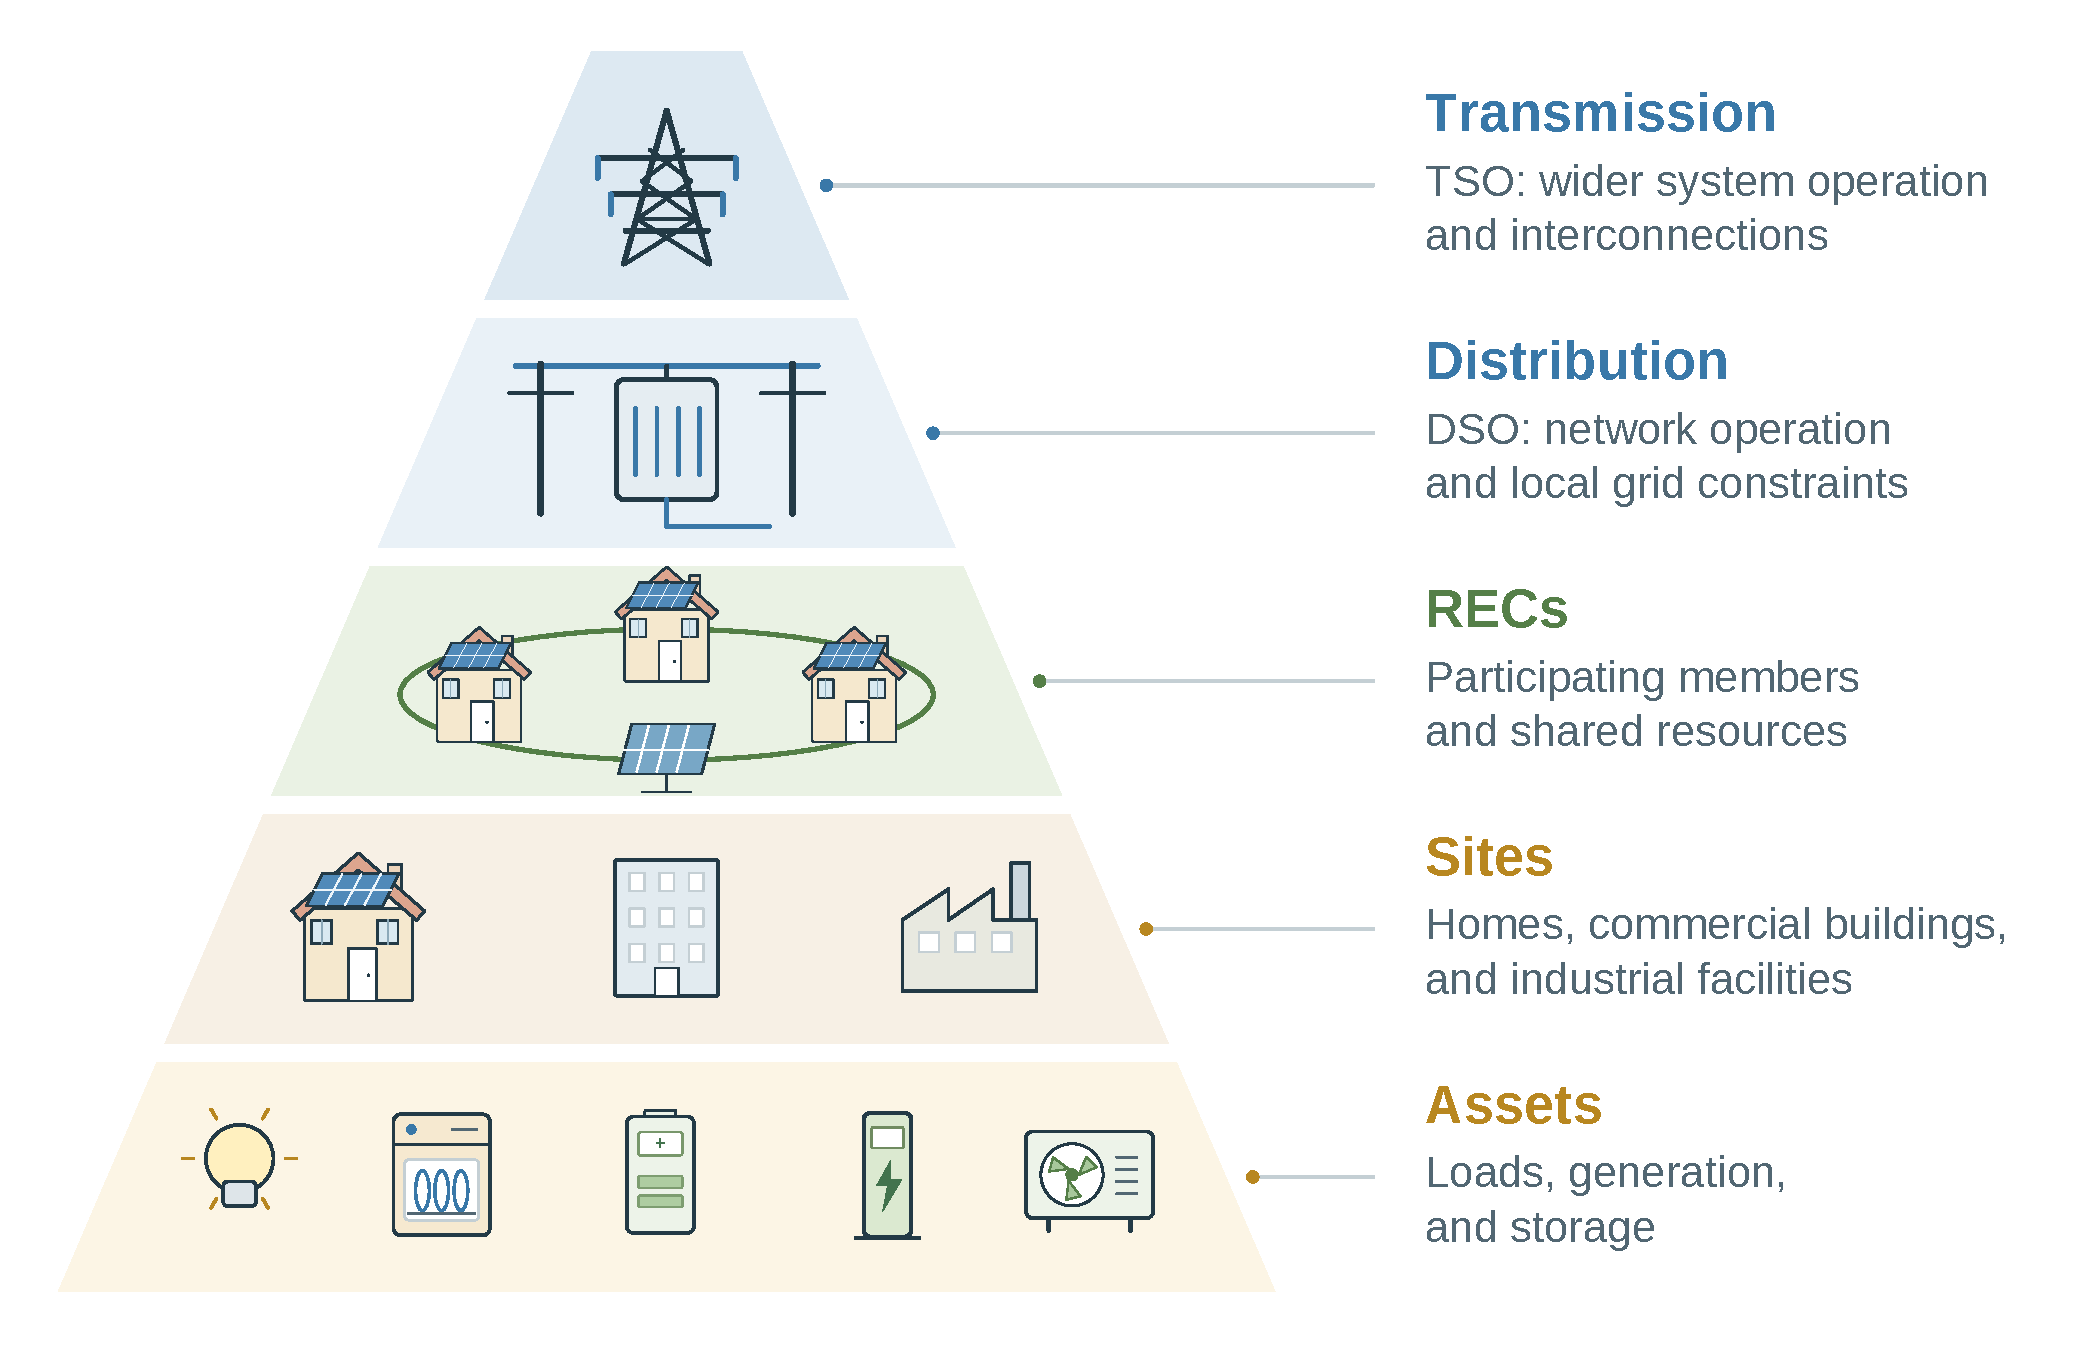
\includegraphics[width=\textwidth]{foundations-community-structure.pdf}
% Author-requested reminder: revise this illustration in a later visual pass.
\captionsetup{labelformat=reviewfigure}
\caption[Levels of organisation around a \gls{rec}]{Levels of organisation and coordination around a \gls{rec}. The pyramid relates assets and sites to \gls{rec} activities and the wider network context; membership arrangements and electrical connections determine the relationships in each installation.}
\label{fig:ch2-community-structure}
\end{figure}

Each level has its own \emph{operating limits}. An individual asset has technical limits associated with its physical design. For example, a charger can supply power within its rated range, and a battery can retain energy within its usable capacity. These limits describe the operation that the asset can support. Service requirements add conditions on its use, such as the energy a vehicle needs for departure or the temperatures occupants require in a room \parencite{hussain2023flexibility}.

At a site, several assets may share a \emph{single-phase} or \emph{three-phase} grid connection \parencite{eredes2025connectionmanual}. The power that can be supplied depends on the connection rating and the current limits of its conductors and protective devices. In a three-phase installation, the loading of each phase also matters, since one phase may reach its limit while capacity remains available on the others. The combined demand must respect these shared limits, even when each asset remains within its own rating. A charger and a heat pump, for example, may each operate at an admissible power while their simultaneous demand exceeds the capacity available to the home.

Similar relationships arise across sites connected to a common feeder or transformer. The scope of a shared electrical limit therefore follows the physical network connections, while \gls{rec} membership identifies the participants whose activities are coordinated.

Within these operating conditions, energy management can pursue objectives at each level. Table~\ref{tab:ch2-objectives-levels} summarises examples of these objectives and the conditions to preserve at each level.

\begin{table}[!htbp]
\centering\small
\caption[Energy-management objectives at different organisational levels]{Examples of energy-management objectives and operating conditions at different levels, synthesised from \textcite{hussain2023flexibility,moret2019energycollectives,reis2021businessmodels,eu2019electricity}.}
\label{tab:ch2-objectives-levels}
\renewcommand{\arraystretch}{1.16}
\begin{tabularx}{\textwidth}{@{}>{\RaggedRight\arraybackslash}p{0.16\textwidth}>{\RaggedRight\arraybackslash}X>{\RaggedRight\arraybackslash}X@{}}
\toprule
\textbf{Level} & \textbf{Examples of objectives} & \textbf{Conditions to preserve}\\\midrule
Asset & Reduce energy losses or wear during operation. & Technical limits and requested service, such as departure energy or thermal comfort.\\\addlinespace[6pt]
Site & Reduce expenditure and peak demand; increase local self-consumption. & Connection capacity and the service requirements of the site's assets.\\\addlinespace[6pt]
\gls{rec} & Increase shared use of renewable production; reduce collective expenditure; distribute benefits fairly. & Members' agreed requirements and applicable shared electrical limits.\\\addlinespace[6pt]
Distribution (\gls{dso}) & Reduce network losses; use network capacity efficiently. & Voltage and loading limits, with continuity of supply.\\\addlinespace[6pt]
Transmission (\gls{tso}) & Operate the wider system efficiently and coordinate exchanges between networks. & Supply--demand balance, frequency, and secure network operation.\\
\bottomrule
\end{tabularx}
\end{table}

\Needspace{3\baselineskip}
Asset characteristics and required services determine the operation available to meet these objectives. The next subsection explains how they define energy flexibility.

\Needspace{7\baselineskip}
\subsection{Asset Operation and Flexibility}
\label{sec:ch2-rec-flexibility}

Assets perform different functions within a site. Appliances and heating equipment create demand, \gls{pv} panels supply electricity, and a stationary battery retains energy for later use. An \gls{ev} combines storage with a mobility requirement and is available to the installation only while connected. Consumption, production, and storage determine the site's exchanges with the grid and the opportunities to adjust its energy use \parencite{hussain2023flexibility,siksnys2019flexoffers}.

\emph{Power} describes the rate of energy transfer, usually expressed here in kilowatts (kW), whereas \emph{energy} describes the amount transferred over an interval, in kilowatt-hours (kWh). A charger operating at 3~kW for one hour transfers 3~kWh at its electrical input. Losses mean that the increase in stored battery energy can be smaller. A storage asset's energy capacity and power rating express separate limits: capacity determines how much it can hold, while the power rating limits how quickly it can charge or discharge. Its \gls{soc} expresses the stored energy relative to a stated reference capacity. These distinctions matter when a service specifies an energy target but the asset accepts a power command.

At the building boundary, \emph{import} is electricity drawn from the external network and \emph{export} is electricity supplied to it. Local generation can meet demand directly, charge storage, or be exported. \emph{Self-consumption} concerns the use of locally generated electricity within the accounting boundary being considered. That boundary may be a building or a \gls{rec}, and the treatment of storage must be stated when the quantity is measured. \gls{rec} sharing allocates locally produced energy among participating members under the applicable arrangement. The allocation is distinct from the physical paths taken by electricity through the network \parencite{moret2019energycollectives,reis2021businessmodels}. A \gls{rec}'s membership and the assets behind one constrained electrical connection can consequently define different groups.

The timing of these exchanges affects the loading of the installation. A \emph{power peak} is the highest power observed over a stated period, with its value depending on the measurement or averaging interval used. Starting the \gls{ev}'s charging while cooking and heating are already drawing power can raise the home's evening import peak. At \gls{rec} level, the peak of the combined demand depends on how closely consumption at different sites coincides.

\emph{Ramping} describes changes in power over time, and a \emph{ramp rate} expresses how quickly power increases or decreases. A charger starting at full power produces an upward change in demand; a gradual increase spreads that change over a longer interval. The size of a peak and the speed of a change describe different features of the same power profile. Adjusting when charging begins and how its power develops can influence both, subject to the energy needed for departure.

\emph{Energy flexibility} is the scope for changing consumption, production, storage, or exchange relative to a reference behaviour while preserving the required service. It depends on the adjustments that the asset permits, its availability, and the time remaining to deliver that service. In the example from Section~\ref{sec:intro-energy-flexibility}, the \gls{ev} arrives at 18:00 with 30\% \gls{soc} and is required to reach 80\% by 08:00. These fourteen hours define the period available to meet the charging request, while the charger's power rating limits how quickly energy can be delivered. The session may allow several hours of delay early in the evening, but much less as departure approaches. Even a controllable charger offers no charging flexibility while the \gls{ev} is absent \parencite{hussain2023flexibility,siksnys2019flexoffers}.

A \emph{FlexOffer} describes this scheduling freedom through an admissible start-time window and an energy profile divided into intervals \parencite{siksnys2019flexoffers,fonseca2022flexloads}. Figure~\ref{fig:ch2-flexoffer} illustrates the two choices: when the charging profile begins and how much energy is assigned to each interval.

\begin{figure}[!htbp]
\centering
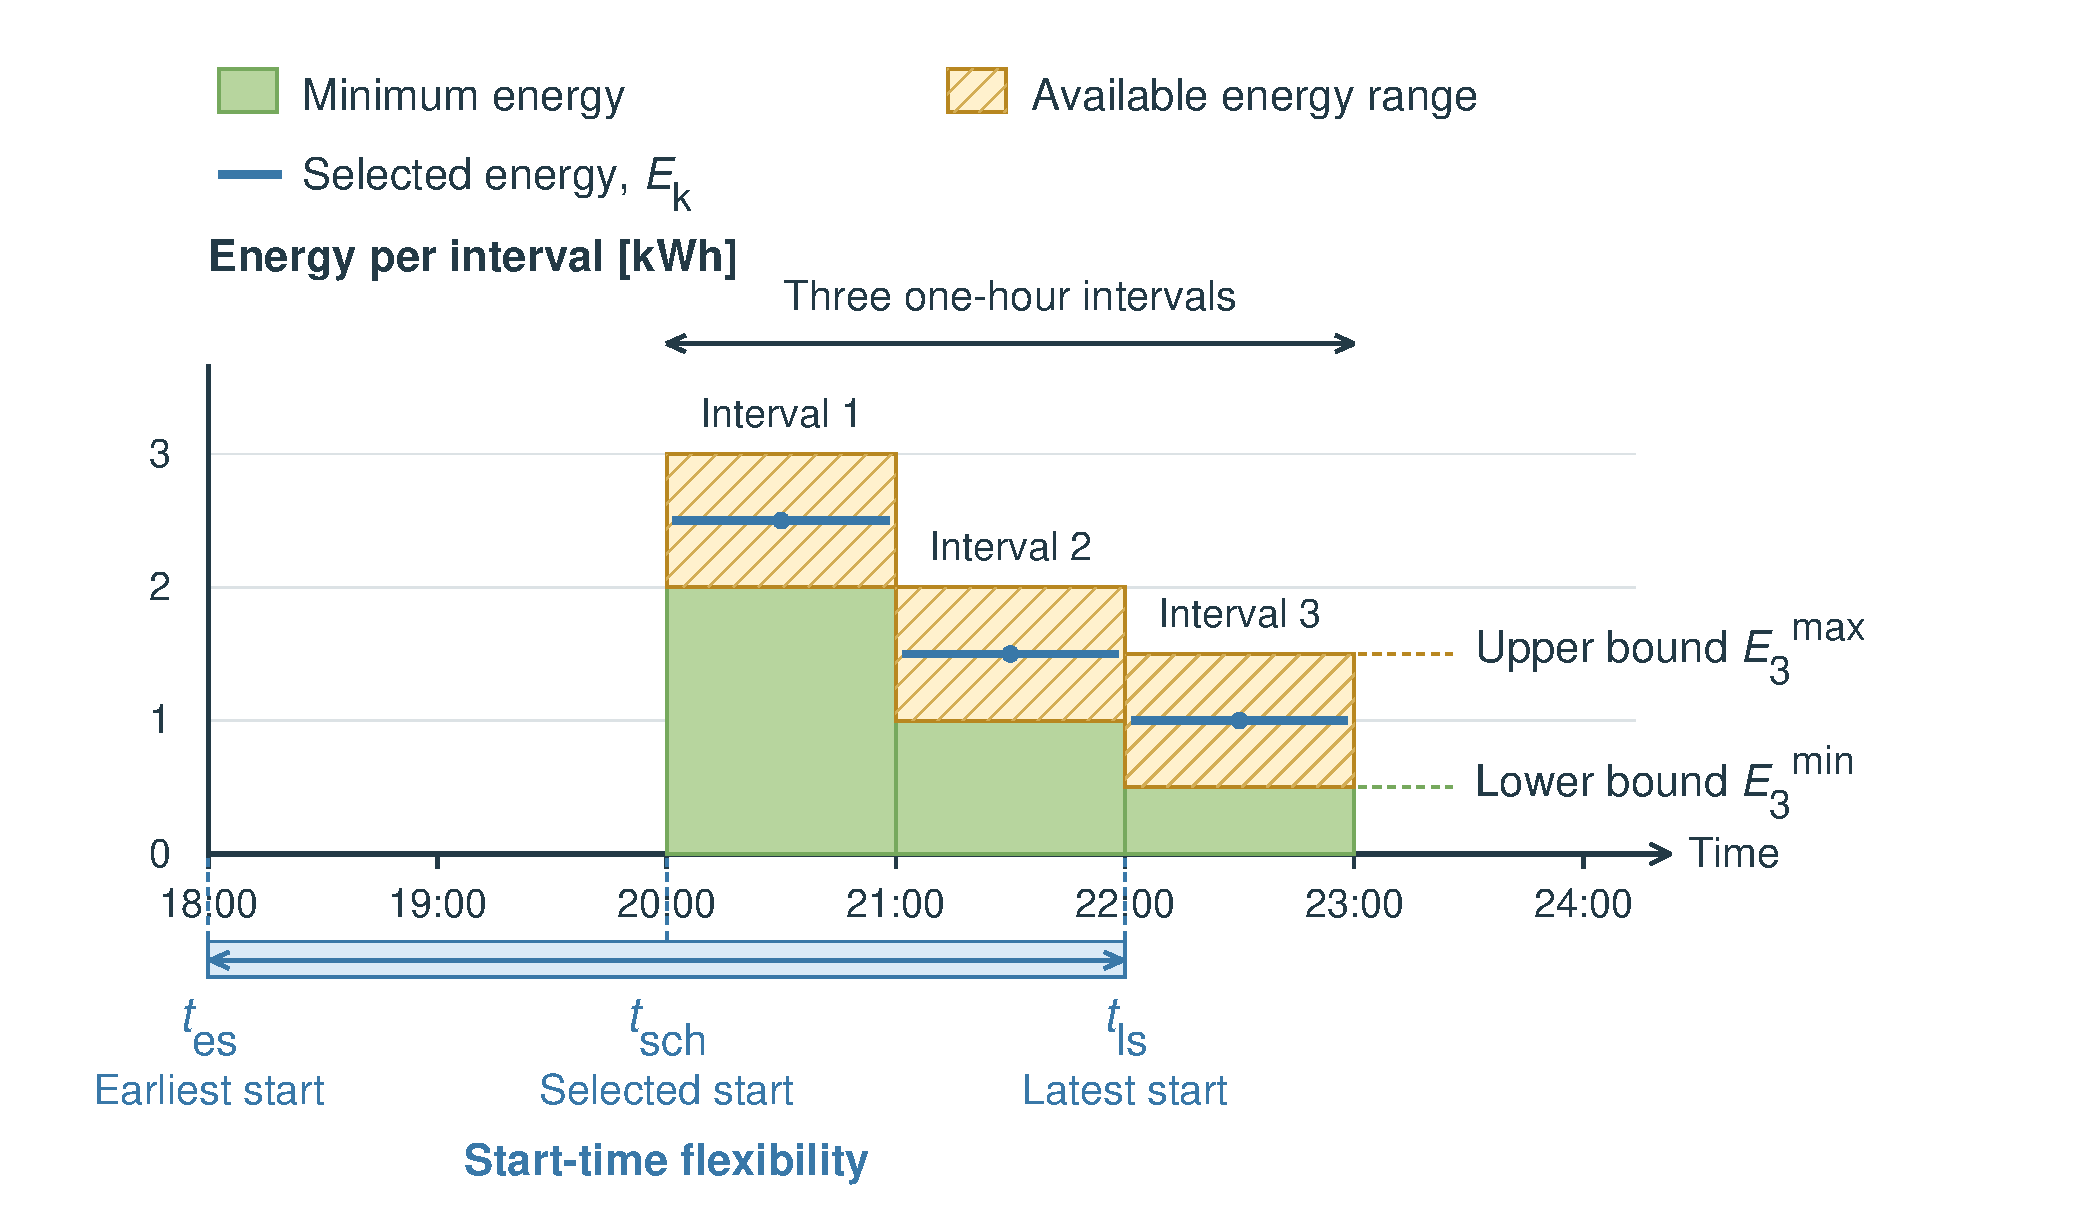
\includegraphics[width=0.90\textwidth]{foundations-flexoffer.pdf}
\caption[Start-time and energy flexibility in a FlexOffer]{Start-time and energy flexibility in a FlexOffer. Redrawn and adapted from \textcite{fonseca2022flexloads}; the values illustrate a profile rather than measured consumption.}
\label{fig:ch2-flexoffer}
\end{figure}

\Needspace{7\baselineskip}
For $N$ intervals of duration $\Delta t$, a FlexOffer $\mathcal F$ is written as:
\begin{equation}
\mathcal F=\left([t_{\mathrm{es}},t_{\mathrm{ls}}],
\left\langle [E_k^{\min},E_k^{\max}]\right\rangle_{k=1}^{N},\Delta t\right).
\label{eq:ch2-flexoffer}
\end{equation}
Here $t_{\mathrm{es}}$ and $t_{\mathrm{ls}}$ are the earliest and latest permitted start times. The ordered profile contains $N$ intervals, each with lower and upper energy bounds $E_k^{\min}$ and $E_k^{\max}$. The index $k$ identifies an interval relative to the profile's start, and $\Delta t$ specifies its duration.

Scheduling selects a start time $t_{\mathrm{sch}}$ and an energy amount $E_k$ for each interval, subject to:
\begin{equation}
t_{\mathrm{es}}\leq t_{\mathrm{sch}}\leq t_{\mathrm{ls}},
\qquad E_k^{\min}\leq E_k\leq E_k^{\max},
\quad k=1,\ldots,N.
\label{eq:ch2-flexoffer-schedule}
\end{equation}
The selected time $t_{\mathrm{sch}}$ positions the whole profile, while each $E_k$ fixes the energy transferred during its corresponding interval. Thus, the horizontal range in the figure represents a choice of start time, and the vertical ranges represent choices of energy. The profile lasts $N\Delta t$, so a service with deadline $t_{\mathrm{dep}}$ requires $t_{\mathrm{sch}}+N\Delta t\leq t_{\mathrm{dep}}$. The latest permitted start must leave enough time for that duration.

Lower and upper bounds on total energy, $E_{\mathrm{tot}}^{\min}$ and $E_{\mathrm{tot}}^{\max}$, couple the interval choices through:
\begin{equation}
E_{\mathrm{tot}}^{\min}\leq\sum_{k=1}^{N}E_k\leq E_{\mathrm{tot}}^{\max},
\label{eq:ch2-flexoffer-total}
\end{equation}
where $E_{\mathrm{tot}}^{\min}$ and $E_{\mathrm{tot}}^{\max}$ bound the energy transferred over the complete profile. An exact energy requirement $E_{\mathrm{req}}$ is represented by setting both bounds to $E_{\mathrm{req}}$. In \gls{ev} charging, this condition preserves the requested total while permitting energy to move between intervals. The target and interval bounds must refer to the same measurement boundary; a target expressed as stored battery energy must also account for charging losses. Together with the vehicle's availability, these conditions determine which schedules can deliver the service. Compatible offers can then be aggregated for scheduling and assigned back to individual assets \parencite{siksnys2019flexoffers}.

The flexibility available from an asset depends on which of these adjustments it supports. Figure~\ref{fig:ch2-resource-flexibility} illustrates fixed, shiftable, and elastic operation through household assets, including stationary storage.

\begin{figure}[!htbp]
\centering
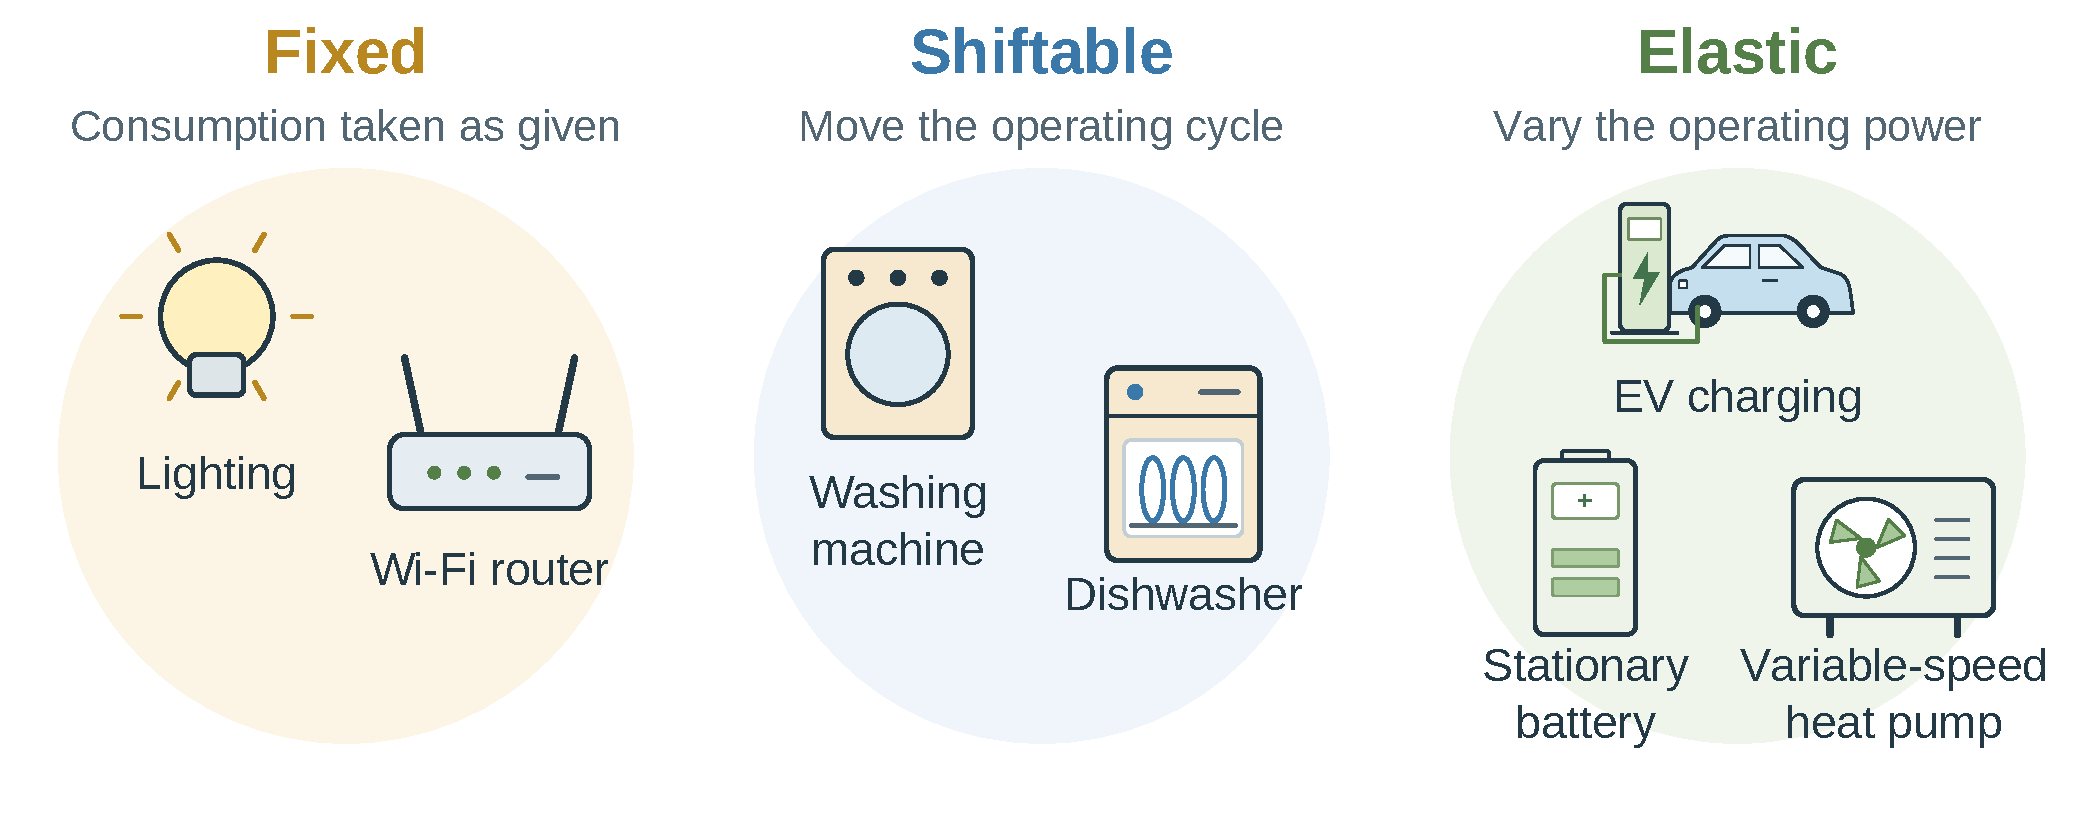
\includegraphics[width=\textwidth]{foundations-resources.pdf}
\caption[Fixed, shiftable, and elastic assets]{Household assets illustrating fixed, shiftable, and elastic operation. Stationary storage provides elastic operation through controllable charging and discharging.}
\label{fig:ch2-resource-flexibility}
\end{figure}

\Needspace{6\baselineskip}
\emph{Fixed} or non-shiftable loads, such as lighting required while a room is occupied, contribute \emph{non-controllable demand}: consumption taken as externally determined at the control timescale. Such demand can still be measured and included when scheduling controllable assets. In the FlexOffer description, a fixed profile has $t_{\mathrm{es}}=t_{\mathrm{sch}}=t_{\mathrm{ls}}$ and $E_k^{\min}=E_k=E_k^{\max}$ for every interval $k$. Both its timing and its energy amounts are therefore specified in advance.

A \emph{shiftable} appliance allows the start of a required operating cycle to move within a time window. A dishwasher loaded after dinner, for example, may begin at different times provided its cycle finishes by morning. Once started, the cycle may need to proceed without interruption. Its temporal flexibility is represented by $t_{\mathrm{es}}<t_{\mathrm{ls}}$, while $E_k^{\min}=E_k^{\max}$ retains the fixed cycle profile in each interval.

An \emph{elastic} or modulable load allows its power to vary within an operating range. An \gls{ev} charger may reduce power during an evening peak and increase it later, changing the interval energy amounts while retaining the departure target. Storage belongs to this category through its controllable charging and discharging power. A stationary battery, for example, can adjust its charging or discharging power within its power limits and usable energy range. This flexibility appears as $E_k^{\min}<E_k^{\max}$ in at least one interval, with Equation~\ref{eq:ch2-flexoffer-total} expressing any total-energy requirement. For storage, the admissible interval choices also depend on the energy retained from earlier decisions and on conversion losses. A fixed start time can coexist with variable energy amounts, while the possibility of pausing operation depends on the asset and service \parencite{fonseca2022flexloads,hussain2023flexibility,siksnys2019flexoffers}.

The schedules permitted by this flexibility can lead to different energy bills and emissions. Their evaluation therefore also depends on the market arrangements and external signals associated with the \gls{rec}'s electricity use.

\Needspace{7\baselineskip}
\subsection{Energy Markets and Decision Signals}
\label{sec:ch2-energy-markets}

\gls{rec} members can purchase electricity to meet their demand and sell production that is available for export, either through individual contracts or collective arrangements. Within the \gls{rec}, energy-sharing agreements can allocate local production among participants, while a \emph{local energy market} can organise transactions between buyers and sellers. These arrangements specify how exchanged energy is valued and how costs and revenues are distributed \parencite{moret2019energycollectives,reis2021businessmodels}.

An \emph{electricity tariff} specifies the prices and charges applied to consumption. A flat energy price applies the same unit rate throughout the day, while a \emph{time-of-use tariff} assigns different rates to predefined periods. Under a \emph{dynamic tariff}, the energy price follows variations in wholesale markets, such as the day-ahead market \parencite{ersetariffstructure,eu2019electricity}. The full bill may also include network charges, taxes, and fixed components.

Environmental information provides another basis for choosing when to use electricity. \emph{Carbon intensity} expresses the greenhouse-gas emissions attributed to a unit of electricity, commonly in grams of CO$_2$ equivalent per kWh. It varies as the generation mix and exchanges between electricity systems change. A production-based value describes generation within an area, while a consumption-based value also accounts for imported electricity. The geographical boundary, time interval, and emissions-accounting method give the signal its meaning when comparing schedules \parencite{electricitymapsmethodology,electricitymapscarbonintensity}.

Using these signals to guide asset operation requires information about the installation and its condition. The next subsection introduces how this information is acquired and the operational conditions that affect its use.


\Needspace{7\baselineskip}
\subsection{Information and Operational Conditions}
\label{sec:ch2-energy-information}

\emph{Data acquisition} obtains measurements and status information from the real-world installation through smart meters, sensors, and asset interfaces. These provide electricity readings, quantities such as room temperature, and operating states or diagnostics, with the measurement points determining which parts of the installation can be observed. Interfaces may also provide \emph{control capabilities}, such as setting charging power, while feedback indicates whether a command was accepted and what the asset delivered \parencite{gopstein2021smartgrid}.

The \emph{sampling interval} is the time between successive measurements, and the \emph{sampling frequency} is the number taken per unit of time. Acquisition, transmission, and storage can follow different schedules: a meter could sample every second, transmit a batch every minute, and retain quarter-hour aggregates, reducing data volume at the cost of temporal detail \parencite{kelly2015ukdale}.

A \emph{timestamp} identifies when a measurement or event occurred, while a separate reception time makes communication delays visible. Consistent clocks and time zones allow records from different assets to be aligned, and an aggregated energy value also needs the interval it covers \parencite{stouffer2023otsecurity}.

A \emph{forecast} estimates a future quantity from information available when it is issued; demand, \gls{pv} production, and weather forecasts may be produced locally or obtained from external services \parencite{nweye2025citylearnv2}. Each forecast needs an issue time and a \emph{forecast horizon}, identifying how far into the future it extends, while retaining successive versions makes it possible to recover the information available at an earlier decision.

\emph{Data quality} concerns the suitability of records for their intended use: \emph{freshness} describes how recent a value is, \emph{validity} concerns its expected format and physical interpretation, and \emph{completeness} concerns the presence of required records.

Table~\ref{tab:ch2-operational-conditions} distinguishes availability, health, dependencies, and degraded operation through the charging example \parencite{stouffer2023otsecurity}.

\begin{table}[!htbp]
\centering\small
\caption[Availability, health, dependencies, and degraded operation]{Operational concepts and their interpretation in the charging example.}
\label{tab:ch2-operational-conditions}
\renewcommand{\arraystretch}{1.16}
\begin{tabularx}{\textwidth}{@{}>{\RaggedRight\arraybackslash}p{0.21\textwidth}>{\RaggedRight\arraybackslash}X>{\RaggedRight\arraybackslash}X@{}}
\toprule
\textbf{Concept} & \textbf{Meaning} & \textbf{Charging example}\\\midrule
\emph{Availability} & Whether an asset can be used for a service at a given time. & The vehicle is connected and charging is authorised.\\\addlinespace[6pt]
\emph{Operational health} & Condition of an asset or supporting component relative to its intended function. & A charger fault reduces the power it can deliver.\\\addlinespace[6pt]
\emph{Operational\newline dependency} & An asset, component, or information source required by a function. & Charging adjusted to site headroom requires a site demand measurement.\\\addlinespace[6pt]
\emph{Degraded operation} & Continuation of a service with reduced capability or performance. & Charging continues under a local limit when demand-based adjustment is unavailable, where local protection supports this mode.\\
\bottomrule
\end{tabularx}
\end{table}

\Needspace{5\baselineskip}
The preceding subsections establish the resources, signals, and information available for \gls{rec} energy management. The next section introduces neural networks, explaining the computational models used to represent learned predictions and decisions before turning to \gls{rl}.

\FloatBarrier
\section{Neural Networks and Learned Representations}
\label{sec:ch2-neural}

The preceding section established the resources, signals, and operating conditions involved in \gls{rec} energy management. Neural networks provide one way to transform this information into predictions or decisions. This section introduces their basic computation and learned representations, preparing the policy and value models used in the \gls{rl} sections and the structured architectures developed in Section~\ref{sec:ch2-structured}.

A \emph{neural network} represents a function $f_\theta$ with learned parameters $\theta$. In the vector formulation used here, the input $x\in\mathbb R^{d_{\mathrm{in}}}$ and output $y=f_\theta(x)\in\mathbb R^{d_{\mathrm{out}}}$ are numerical vectors; $d_{\mathrm{in}}$ and $d_{\mathrm{out}}$ count their components. Measurements supply numerical features, while categories require a numerical encoding. For a charger, three input components might represent \gls{soc}, time until departure, and electricity price, with one output component representing a power request \parencite{goodfellow2016deep}.

A \emph{feed-forward network} passes information from input to output through successive transformations. A \gls{mlp} uses dense layers, in which each unit combines all components from the preceding layer. Between input and output, one or more \emph{hidden layers} compute intermediate numerical vectors.

\Needspace{6\baselineskip}
The transformation producing the vector $h^{(\ell)}$ at layer $\ell$ is:
\begin{equation}
h^{(\ell)}=\sigma_\ell\!\left(W^{(\ell)}h^{(\ell-1)}+b^{(\ell)}\right),
\qquad h^{(0)}=x,
\label{eq:ch2-neural-layer}
\end{equation}
where $W^{(\ell)}$ contains the learned weights, $b^{(\ell)}$ is a bias vector, and $\sigma_\ell$ is the layer's activation function. The weights combine the incoming values, the bias supplies an offset, and the activation transforms the result before it passes to the next layer.

Nonlinear activations allow stacked layers to represent nonlinear relationships. A \gls{relu}, for example, replaces negative values by zero and leaves non-negative values unchanged. Other common activations include the sigmoid, with outputs between zero and one, and the hyperbolic tangent, with outputs between $-1$ and $1$. These functions produce continuous values rather than binary on/off decisions \parencite{goodfellow2016deep}.

The output's interpretation depends on the task. A numerical output can specify a continuous quantity such as charging power. For a discrete choice, such as charge or wait, the network can produce a vector of scores; a softmax transformation converts them into probabilities, from which a choice is selected. Section~\ref{sec:ch2-modular-policies} returns to these action mappings.

A dense network is configured for a fixed number of input and output components. In the charging example, changing the \gls{soc} changes one of the three input values. Adding battery temperature would instead require a fourth input and a corresponding change to the network's input connections. Section~\ref{sec:ch2-structured} introduces ways to organise changing collections of resources, including padding, entity representations, and attention-based architectures.

Figure~\ref{fig:ch2-neural} follows the charging example through three input components, four hidden components, and one output. The four hidden values form a \emph{learned representation} of the input, computed inside the network and passed to its output layer. They combine the supplied features using learned parameters; each hidden value need not correspond to a named physical quantity.

\begin{figure}[!htbp]
\centering
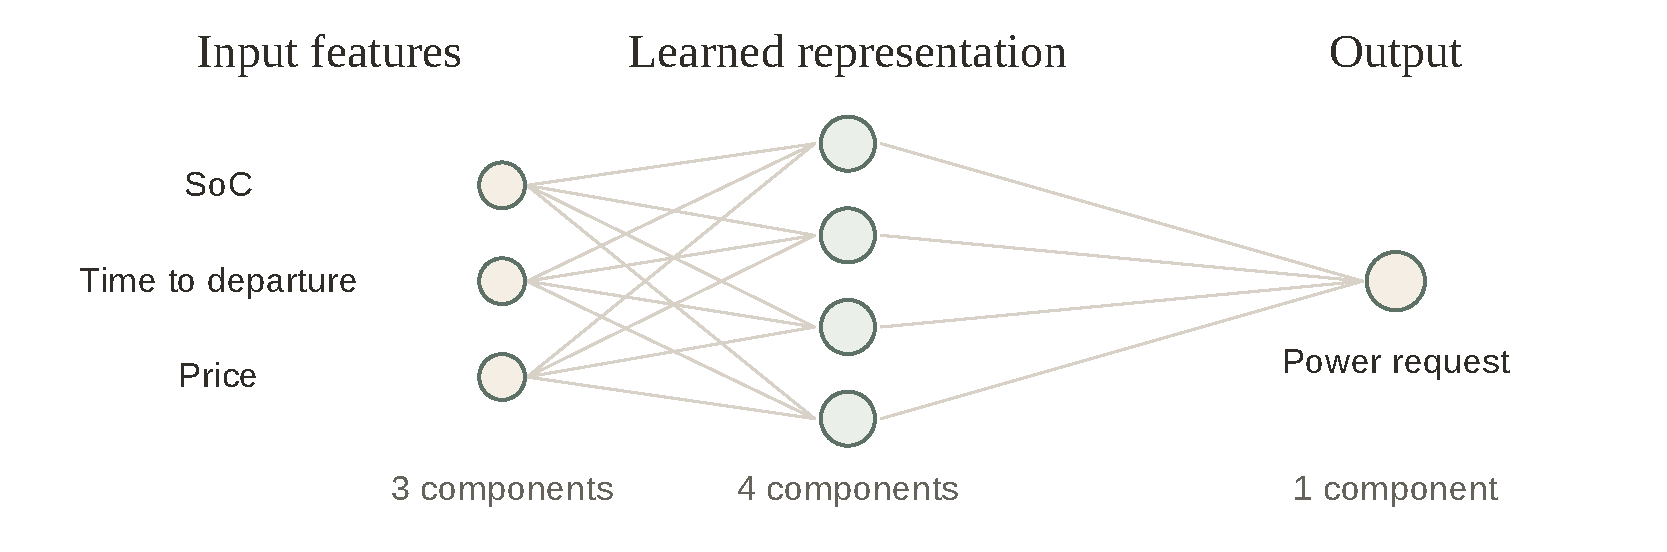
\includegraphics[width=\textwidth]{figures/foundations-neural.pdf}
\caption{A feed-forward network mapping three charging-related features through a learned representation to one output. The illustrated layer widths are architectural choices. Original illustration based on \textcite{goodfellow2016deep}.}
\label{fig:ch2-neural}
\end{figure}

\Needspace{3\baselineskip}
Such a representation is often called an \emph{embedding} when used as a numerical description for further computation. The part of the network that maps the inputs into this representation acts as an \emph{encoder}; a \emph{decoder} maps it into the required output. In the figure, the encoder produces the four hidden values and the decoder uses them to obtain the power request. Section~\ref{sec:ch2-structured} develops these roles for collections of resources.

Learning adjusts the parameters to minimise a \emph{loss function}. With known target outputs, the loss can measure the discrepancy between predictions and targets. \emph{Backpropagation} computes how the loss changes with the parameters, and an optimisation procedure uses these derivatives to update them \parencite{goodfellow2016deep}. Applying the trained network is \emph{inference}. During fixed-policy execution, new measurements produce new outputs while the parameters remain unchanged.

This section established how a network transforms numerical inputs into outputs and how its parameters are learned. The next section introduces \gls{rl}, where actions and their consequences supply the experience used to learn a decision rule.

\FloatBarrier
\Needspace{10\baselineskip}
\section{Reinforcement Learning}
\label{sec:ch2-rl}

\gls{rl} is based on the idea that a decision-maker can improve its choices by experiencing their consequences. Some \gls{rl} methods use the neural networks introduced in Section~\ref{sec:ch2-neural} to represent decision rules or estimates of future reward. This section introduces the foundations needed to understand the learning methods used in this thesis, covering the agent--environment interaction, the objective pursued over time, and the mechanisms used to learn a policy.

\Needspace{7\baselineskip}
\subsection{Sequential Decision-Making and Partial Observability}
\label{sec:ch2-mdp}
\label{sec:ch2-pomdp}

In sequential decision-making, an action can change both the immediate outcome and the choices available later. \gls{rl} represents this process as an interaction between an \emph{agent}, which selects actions, and an \emph{environment}, which responds to them.

\Needspace{7\baselineskip}
A \gls{mdp} $\mathcal M$ formalises this interaction \parencite{sutton2018rl}:
\begin{equation}
\mathcal M=(\mathcal S,\mathcal A,P,R,\gamma,\rho_0),
\label{eq:ch2-mdp}
\end{equation}
where $\mathcal S$ and $\mathcal A$ are the state and action spaces, $P(s'\mid s,a)$ is the transition distribution, and $R(s,a,s')$ is the expected immediate reward associated with a transition. The discount factor $\gamma$ determines the weighting of future rewards, and $\rho_0$ specifies the initial-state distribution.

At decision step $t$, the \emph{state} $s_t$ describes the conditions relevant to the task, and the \emph{action} $a_t$ specifies the agent's choice. The \emph{Markov property} means that $s_t$ summarises the information from past interactions needed to predict the next state $s_{t+1}$ and reward $r_t$, given $a_t$. Once $s_t$ and $a_t$ are known, the earlier sequence of states and actions adds no further information to that prediction. In the fully observable \gls{mdp} formulation, the agent has access to $s_t$ when choosing $a_t$ \parencite{sutton2018rl}.

A \emph{policy} $\pi$ determines how the agent selects $a_t$ from $s_t$. Applying $a_t$ leads to $s_{t+1}$ and a \emph{reward} $r_t$: a scalar signal that rates the outcome according to the task's objective, with larger values expressing more favourable outcomes. For a cost-minimisation objective, for example, the reward can be the negative cost incurred during the transition. Here $r_t$ denotes the signal received after $a_t$, while $R(s,a,s')$ gives its expected value for a specified transition \parencite{sutton2018rl}. Figure~\ref{fig:ch2-rl-cycle} illustrates this cycle, with $s_{t+1}$ providing the information for the next decision.

\begin{figure}[!htbp]
\centering
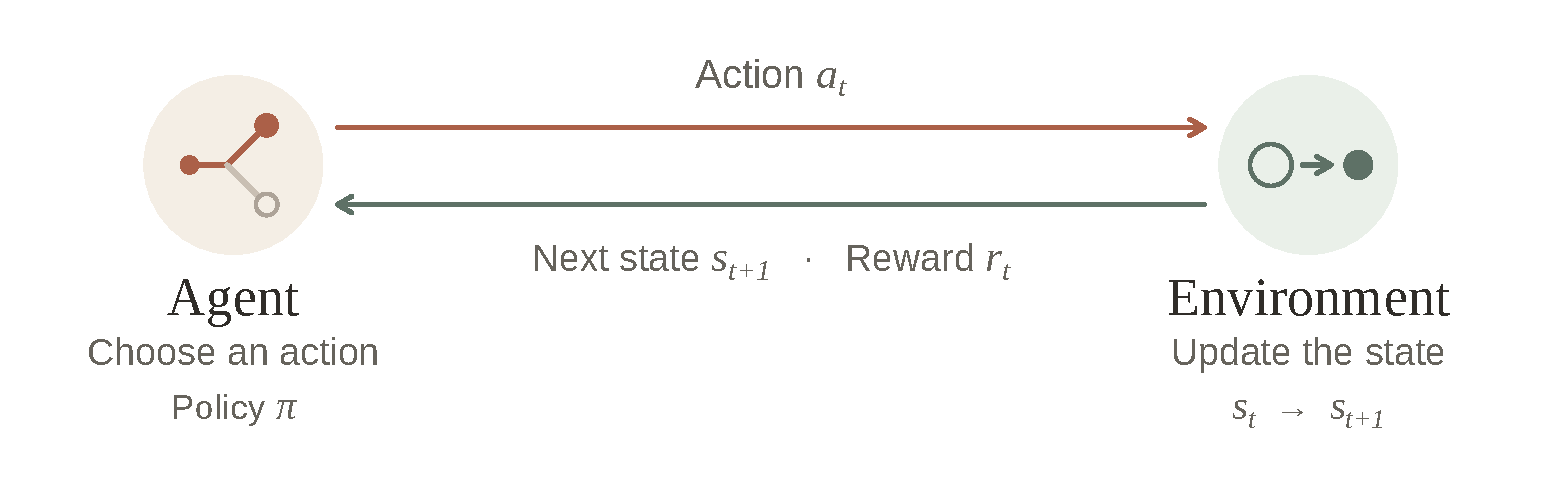
\includegraphics[width=0.86\textwidth]{figures/foundations-rl-cycle.pdf}
\caption{Agent--environment interaction in a fully observable \gls{mdp}. The reward $r_t$ follows action $a_t$, and the next state $s_{t+1}$ becomes available to the agent. Original illustration based on the formulation of \textcite{sutton2018rl}.}
\label{fig:ch2-rl-cycle}
\end{figure}

\gls{ev} charging illustrates this formulation within a \gls{rec}. The agent controls charging at a site (for example, a household), while the environment includes the vehicle, charger, and the site's electrical installation. The state $s_t$ includes the stored energy, departure target, time remaining, and relevant electrical conditions; $a_t$ is the selected charging power. Including the remaining time distinguishes the same battery \gls{soc} early in the evening from that \gls{soc} shortly before departure. Charging increases the stored energy as the remaining time decreases, producing $s_{t+1}$, while $r_t$ can reflect the cost of the energy delivered during the interval.

\Needspace{3\baselineskip}
In a real-world installation, the measurements available through sensors and interfaces determine which conditions the agent can observe, with noise or delays introducing further uncertainty \parencite{dulacarnold2021realworld}. The agent receives an \emph{observation} $o_t$ containing the available information about $s_t$. The task is \emph{partially observable} when this information provides an incomplete or uncertain description of the state relevant to its decisions, leaving some conditions affecting the outcome hidden from the agent.

\Needspace{7\baselineskip}
A \gls{pomdp} $\mathcal M_{\mathrm{PO}}$ extends the \gls{mdp} with an observation space and an observation model \parencite{kaelbling1998pomdp}:
\begin{equation}
\mathcal M_{\mathrm{PO}}=(\mathcal S,\mathcal A,P,R,\mathcal O,Z,\gamma,\rho_0),
\label{eq:ch2-pomdp}
\end{equation}
where $\mathcal O$ is the space of observations $o_t$ and $Z(o_{t+1}\mid s_{t+1},a_t)$ describes the distribution of the next observation after action $a_t$ leads to state $s_{t+1}$. The remaining components retain their \gls{mdp} meanings. The observation model describes how information about the underlying state becomes available to the agent.

For the charging agent, $o_t$ might contain measured charging power and the reported departure time while omitting battery \gls{soc}. The agent can observe the rate of energy delivery, but the energy already stored remains hidden, leaving uncertainty about how much more charging is needed. The interaction still follows the cycle in Figure~\ref{fig:ch2-rl-cycle}, with $o_{t+1}$ replacing direct access to $s_{t+1}$; the agent can use past observations and actions to help infer the missing state information.

A \emph{belief state} summarises this history as a probability distribution over possible states $s_t$, updated as actions are taken and new observations arrive. Given the \gls{pomdp} model and an initial belief, it provides sufficient information for selecting actions, although exact updates can be computationally demanding \parencite{kaelbling1998pomdp}. Practical policies can instead retain a window of past observations or use recurrent memory to integrate information over time \parencite{hausknecht2015drqn}.

The next subsection explains how the rewards received across successive decisions are combined into a return, and how value functions use that return to assess a policy over the course of a task, including consequences that only emerge after several actions.

\Needspace{7\baselineskip}
\subsection{Returns, Episodes, Value Functions, and Policies}
\label{sec:ch2-return-value}

In the interaction described above, the agent receives a reward $r_t$ after applying action $a_t$, giving feedback on that transition. Evaluating the policy requires following the consequences of successive choices, which the \emph{return} $G_t$ captures by accumulating rewards over the remainder of an episode or, for a continuing task, over a longer horizon.

An \emph{episode} groups successive interactions over a defined period. In a \gls{rec}, this may cover a day or a year of chronological data, containing many charging sessions and other asset operations. Lowercase $t$ indexes a decision step, while uppercase $T$ marks the end of the sequence, after the last action at $T-1$. A \emph{terminal state} marks the end of the modelled task; a selected data window can also end while the real-world operation continues.

\Needspace{7\baselineskip}
Over an episode ending at $T$, the discounted return $G_t$ from step $t$ combines the previously introduced rewards $r_t$ as:
\begin{equation}
G_t=\sum_{k=0}^{T-t-1}\gamma^k r_{t+k}.
\label{eq:ch2-return}
\end{equation}
Here $r_{t+k}$ is the reward received $k$ steps after $t$, weighted by $\gamma^k$, and the sum ends at the last transition before $T$. Continuing tasks can use an infinite discounted sum with $0\leq\gamma<1$, or an average-reward formulation. In finite tasks, $\gamma=1$ retains equal weight for rewards throughout the remaining episode when the return is well defined \parencite{sutton2018rl}.

If charging rewards are simply negative electricity costs and $\gamma=1$, $G_t$ is the negative total cost from the current step to the end of the episode. A discount factor below one reduces the contribution of distant rewards, with its effect depending on the decision interval. The same numerical value produces a different effective time horizon at one-minute and one-hour resolution.

\Needspace{6\baselineskip}
A stochastic policy $\pi(a\mid s)$ gives a distribution over actions; a deterministic policy $\mu(s)$ selects one action. The \emph{state-value function} $V^\pi(s)$ and \emph{action-value function} $Q^\pi(s,a)$ describe expected returns under $\pi$:
\begin{align}
V^\pi(s)&=\mathbb E_\pi[G_t\mid s_t=s],\\
Q^\pi(s,a)&=\mathbb E_\pi[G_t\mid s_t=s,a_t=a].
\label{eq:ch2-value-functions}
\end{align}
Here $\mathbb E_\pi$ denotes expectation under policy $\pi$, conditional on the current state $s$ or state--action pair $(s,a)$. It accounts for transitions and, where applicable, policy randomness. For finite-horizon problems these functions can depend on the remaining time; the notation suppresses this dependence when time is included in the state. For the \gls{ev}, $V^\pi(s)$ estimates the return from following the charging policy from the current conditions, while $Q^\pi(s,a)$ estimates the return from first choosing a particular charging power and then following that policy.

The Bellman relation expresses $Q^\pi(s,a)$ through the reward obtained now and the value of what follows:
\begin{equation}
Q^\pi(s,a)=\mathbb E\!\left[r_t+\gamma
\mathbb E_{a'\sim\pi(\cdot\mid s_{t+1})}Q^\pi(s_{t+1},a')
\mid s_t=s,a_t=a\right].
\label{eq:ch2-bellman}
\end{equation}
The outer expectation averages over the resulting reward $r_t$ and next state $s_{t+1}$; the inner expectation averages over the next action $a'$ drawn from $\pi$. At a terminal transition, the continuation value is zero. This recursion allows observed rewards and estimated future values to inform the same learning update. If the charging reward includes a penalty for energy missing at departure, an action with a small immediate cost can have a poor value because it leaves insufficient time to complete the service. The value function carries that later consequence into the present decision through the specified reward.

The \emph{advantage} $A^\pi(s,a)=Q^\pi(s,a)-V^\pi(s)$ compares an action with the policy's expected performance at the same state. For the \gls{ev}, a positive advantage means that the selected charging power has a higher expected return than the policy achieves on average from those conditions. This relative learning signal can reduce variability when updating a policy.

These comparisons depend on what the reward treats as a favourable outcome, which leads to the next subsection's question of how to construct that signal from the task's objectives.

\Needspace{7\baselineskip}
\subsection{Reward Design and Objective Specification}
\label{sec:ch2-reward}

The preceding subsection accumulated rewards into a return and used expected returns to evaluate a policy. The next step is to specify the reward function $R$ introduced in the \gls{mdp}, which determines what each transition contributes to that evaluation. In a \gls{rec}, this means translating objectives such as reducing expenditure, delivering the requested departure energy, and maintaining thermal comfort into the learning signal. These objectives were introduced at the asset, site, and \gls{rec} levels in Section~\ref{sec:ch2-rec-members} and Table~\ref{tab:ch2-objectives-levels}.

\Needspace{7\baselineskip}
Several such objectives can contribute to a single \emph{composite reward} $r_t$ through a weighted sum \parencite{roijers2013multiobjective}:
\begin{equation}
r_t=\sum_{j=1}^{m} w_j f_j(s_t,a_t,s_{t+1}),
\label{eq:ch2-composite-reward}
\end{equation}
where $m$ is the number of components, $f_j$ is the signal for outcome $j$, and $w_j\geq 0$ sets its weight. Each $f_j$ is expressed so that larger values are preferred; costs and shortfalls can therefore enter as negative terms. The components can conflict. Postponing \gls{ev} charging may reduce expenditure while increasing the energy missing at departure, so a gain in one term can be offset by a loss in another. The weights express the relative importance of these outcomes in the combined signal.

The numerical scale of each $f_j$ also affects this balance. For components measured in euros and kWh, the weights must account for both their numerical ranges and their intended relative importance. Normalisation can provide a reference scale, while changing either that scale or the weights changes the trade-off.

A service requirement can enter both the reward and the constraints governing the decision. A departure-energy penalty encourages learning to value readiness, while a constraint can require a charging schedule to deliver the requested energy whenever the available time and capacity permit. Electrical limits likewise restrict admissible actions. Reward terms guide the preference among outcomes; enforcing a requirement needs a mechanism that restricts the decisions applied, as introduced in Section~\ref{sec:ch2-constrained-foundations}.

Reward design also determines when feedback is supplied. A \emph{sparse} reward occurs only at selected events, such as task completion or failure, whereas a \emph{dense} reward provides more frequent feedback throughout the interaction. Sparse feedback can express the final outcome directly, although identifying which earlier decisions contributed to it becomes more difficult. In the charging example, expenditure may contribute at every interval while readiness is assessed at each departure within the episode; discounting then affects the relative influence of these contributions. Dense feedback can help learning recognise progress, but rewarding an intermediate quantity may favour behaviour that improves that quantity while weakening the final outcome \parencite{sutton2018rl}.

\Needspace{8\baselineskip}
\emph{Reward shaping} supplies additional feedback during learning to make useful intermediate progress easier to recognise. For an \gls{ev}, this can help relate successive charging decisions to the energy needed at departure, before that service is finally assessed. In potential-based shaping, a function $\Phi$ assigns a numerical measure of progress to each state and defines a shaped reward $r_t^{\Phi}$ \parencite{ng1999shaping}:
\begin{equation}
r_t^{\Phi}=r_t+\gamma\Phi(s_{t+1})-\Phi(s_t).
\label{eq:ch2-potential-shaping}
\end{equation}
Here $\Phi(s_t)$ and $\Phi(s_{t+1})$ evaluate the current and next states, and $\gamma$ is the discount factor already used in the return. Their discounted difference is added to the original reward $r_t$. In the charging example, $\Phi$ could assign higher values as the energy shortfall decreases, providing feedback about progress between successive decisions.

The reward function now specifies the feedback available to the learning process, while the return combines that feedback over time. The next subsection explains how experience from successive interactions is used to estimate values and improve the policy.

\Needspace{7\baselineskip}
\subsection{Learning from Experience}
\label{sec:ch2-experience}
\label{sec:ch2-policy-gradient}

Learning uses the feedback defined above to improve subsequent decisions. Each interaction records the conditions faced by the agent, the action it applied, and the resulting reward and next state. In the \gls{rec} example, a charging decision reveals how the selected power affects stored energy, electricity expenditure, and the time remaining to meet the departure target.

\emph{Value-based learning} estimates the return associated with states or actions and uses those estimates to choose decisions. For the charging agent, this means learning how promising charging now, waiting, or selecting a lower power is from the current conditions, considering their consequences through the rest of the episode. Experience revises these estimates, helping the agent choose actions with higher expected return \parencite{sutton2018rl,watkins1992qlearning}.

\Needspace{8\baselineskip}
\emph{Policy-based learning} adjusts the rule that selects actions. For example, the charging agent can learn to assign a higher probability to power settings that perform better than expected in the conditions it encounters. The parameters $\theta$ control this rule, represented by a differentiable policy $\pi_\theta$. The policy-gradient principle relates an improvement in expected return to terms of the form:
\begin{equation}
\mathbb E\!\left[\nabla_\theta\log\pi_\theta(a_t\mid s_t)
A^{\pi_\theta}(s_t,a_t)\right],
\label{eq:ch2-policy-gradient}
\end{equation}
where $\nabla_\theta$ differentiates with respect to the policy parameters, $\log\pi_\theta$ is the log-probability of the selected action, and $A^{\pi_\theta}$ is its advantage. The expectation averages over the states and actions used by the method. The advantage guides the update towards making better-than-expected actions more likely and worse-than-expected actions less likely in comparable conditions \parencite{sutton1999policygradient}.

An \emph{actor--critic} method brings these two roles together. The actor selects an action, while the critic estimates the values used to assess it and guide learning. In the \gls{rec} example, the actor chooses charging power and the critic helps judge whether that choice improves the expected return.

\emph{Exploration} allows the agent to learn about alternatives to its current preferred action. A charging agent might try two permitted power levels in similar conditions to learn how their consequences differ. A stochastic policy can sample different actions, while a deterministic policy can use a perturbation during experience collection. In a real-world installation, these choices must respect the available operating limits.

\emph{Entropy regularisation} encourages a stochastic policy to retain variety in its action choices while improving return. For the charging agent, this can help avoid concentrating too early on a single power setting. Its coefficient controls the strength of that encouragement \parencite{haarnoja2018sac}.

\emph{On-policy} and \emph{off-policy} learning describe how the policy that collects experience relates to the one being learned. An on-policy charging agent learns from decisions made with the policy currently being improved. An off-policy method can also learn from decisions made by an earlier or different controller. The distinction identifies which policy generated the data; online and offline learning instead distinguish whether new interactions are collected during learning.

A \emph{replay buffer} stores transitions so that an off-policy method can reuse them in later updates. A recorded charging decision can therefore contribute to learning more than once, even after the controller has changed. Learning entirely from a fixed archive is developed in Section~\ref{sec:ch2-offline}.

Building on the learning methods described above, the next subsection explains how knowledge from an existing controller can help the agent learn useful behaviour, and how operational constraints govern the choices it can apply during learning and subsequent operation.

\Needspace{7\baselineskip}
\subsection{Prior Knowledge and Constrained Decisions}
\label{sec:ch2-constrained-foundations}

The learning process described above can begin with knowledge of how the installation is already operated. In a \gls{rec}, a \gls{rbc} may already schedule charging using electricity prices, battery \gls{soc}, and departure requirements. This \emph{prior knowledge} can help the agent learn useful behaviour through examples, guidance during exploration, or adjustments to an existing control rule.

\emph{\gls{bc}} learns to reproduce a controller's or expert's decisions from demonstrations that pair the conditions encountered with the actions chosen. For the charging agent, these examples associate the vehicle's needs and the electricity price with a selected charging power. Supervised learning fits the policy to these choices; when rewards and subsequent states are also recorded, the transitions can support \gls{rl} \parencite{ross2011dagger}.

\emph{Guided exploration} uses existing knowledge to direct the agent towards promising actions while collecting experience. A controller's recommended charging power, for example, can provide a starting point for trying nearby permitted power levels. The resulting rewards and state changes then inform the learner's own decisions.

\emph{Residual learning} retains the existing controller as part of the decision rule and learns an adjustment to its output. In the charging example, the controller supplies a reference power and the learned policy increases or decreases that value in response to the current conditions \parencite{johannink2019residual}.

These ways of using prior knowledge operate within the installation's physical and service requirements. \emph{Constraints} express which actions or sequences of actions are admissible. A constrained \gls{mdp} can maximise expected reward subject to budgets $d_j$ on expected accumulated costs $c_j$, written generically as:
\begin{equation}
\mathbb E_\pi\!\left[\sum_t\gamma^t c_j(s_t,a_t)\right]\leq d_j,
\qquad j=1,\ldots,m,
\label{eq:ch2-cmdp}
\end{equation}
where $j$ indexes the $m$ constraints, $c_j(s_t,a_t)$ is the cost at step $t$, and $d_j$ is its permitted accumulated budget. The expectation averages discounted costs over trajectories generated by $\pi$ \parencite{achiam2017cpo}. Such a condition concerns an expectation over trajectories. An instantaneous equipment limit instead applies to every relevant command, and a deadline condition depends on a sequence of decisions. These meanings require different enforcement mechanisms.

An action mask can remove inadmissible discrete choices before selection. For continuous decisions, a projection or safety filter can map a proposed action into an admissible set determined by a constraint model. A supervisory controller may supply a fallback when the proposed decision cannot be used \parencite{dalal2018safe,elsayedaly2021shielding}.

This section introduced how an agent learns a policy from rewards and experience, with prior knowledge and constraints guiding its decisions. The next section extends these foundations to \gls{marl}, where agents interact within a shared environment such as a \gls{rec}.

\Needspace{8\baselineskip}
\FloatBarrier
\section{Multi-Agent Reinforcement Learning}
\label{sec:ch2-marl}

The preceding section considered how one agent learns to act on its environment. In \gls{marl}, several agents learn while their decisions jointly affect that environment. Consider a \gls{rec} in which each site has an agent controlling its \gls{ev} charging. If two agents charge during the same low-price period, their simultaneous charging can create a \gls{rec} demand peak. This section extends the decision model to such interactions, then explains how learning is organised and how individual decisions contribute to a shared outcome.

\Needspace{7\baselineskip}
\subsection{Markov Games and Multi-Agent Objectives}
\label{sec:ch2-markov-games}

The \gls{mdp} described one agent's action at each step. With several agents, the environment responds to their combined choices, represented by a \emph{joint action}. A Markov game $\mathcal G$, also called a stochastic game, expresses this interaction \parencite{shapley1953stochastic,littman1994markovgames}. A discounted formulation is:
\begin{equation}
\mathcal G=\left(\mathcal N,\mathcal S,
\{\mathcal A_i\}_{i\in\mathcal N},P,
\{R_i\}_{i\in\mathcal N},\gamma,\rho_0\right),
\label{eq:ch2-markov-game}
\end{equation}
where $\mathcal N=\{1,\ldots,n\}$ is the fixed agent set and $\mathcal A_i$ is agent $i$'s action space. The joint action $a=(a_1,\ldots,a_n)$ belongs to the product of those spaces. The transition distribution is now $P(s'\mid s,a)$, and each agent has an expected reward $R_i(s,a,s')$. As in the \gls{mdp}, $\mathcal S$ is the state space, $\gamma$ the discount factor, and $\rho_0$ the initial-state distribution.

In the \gls{rec} example, $a_{i,t}$ is the charging power selected at site $i$, and $a_t$ collects all sites' choices at that step. Their combined charging changes the vehicles' stored energy and the \gls{rec}'s total demand. Each agent's reward can therefore depend on both its own choice and the choices made elsewhere in the \gls{rec}.

A \emph{fully cooperative} game gives all agents the same reward and a common performance objective. For the charging agents, that reward could combine \gls{rec} electricity expenditure, peak demand, and the energy missing at vehicle departures. Each site's decisions then contribute to the outcome that all agents learn to improve.

A \emph{general-sum} game allows agents to have different rewards, expressing objectives that may partly coincide and partly conflict. In a \gls{rec}, members may pursue individual expenditure targets alongside a \gls{rec} objective. In a \emph{zero-sum} game, the agents' rewards sum to zero for every transition. With two agents, one agent's reward is therefore the negative of the other's \parencite{wang2022coopcompetitive,moret2019energycollectives}.

The community-control problem studied in this thesis assumes agreement on the collective objectives and individual service commitments to be considered. Reducing a community peak, for example, is pursued alongside the energy required by each vehicle at departure. These commitments enter the control formulation through constraints, reward terms, and assessment of the service delivered. Cooperation is therefore a choice in the formulation of the control problem. A common reward defines the fully cooperative case, while formulations combining local and community rewards retain agent-specific objectives whose effects on coordination must be assessed. Each controller's reward construction is specified in the corresponding method description. Assessing individual outcomes also remains necessary to establish how the benefits and burdens of coordination are distributed.

Under \emph{partial observability}, each agent receives an observation $o_{i,t}$ that does not necessarily reveal all the state information relevant to its decisions. The charging agent might observe its own vehicle's \gls{soc} and departure time together with a published electricity price. Its action can depend on its local history $h_{i,t}$ of observations and previous actions.

\Needspace{8\baselineskip}
The individual policies together define the joint policy $\pi$. When agents sample independently conditional on their local histories, it factorises as:
\begin{equation}
\pi(a_t\mid h_t)
=\prod_{i\in\mathcal N}\pi_i(a_{i,t}\mid h_{i,t}).
\label{eq:ch2-joint-policy}
\end{equation}
Here $a_t=(a_{1,t},\ldots,a_{n,t})$ and $h_t=(h_{1,t},\ldots,h_{n,t})$ collect the agents' actions and local histories, and $\pi_i$ is agent $i$'s policy. The product combines the probabilities of their individual choices into the probability of the joint action. In the example, each site's agent chooses a charging power from its available information, and those choices are applied together.

A \gls{decpomdp} formalises cooperation under a common reward, with agents acting from local observations and action histories \parencite{oliehoek2016decpomdp}.

\Needspace{7\baselineskip}
\subsection{Learning and Execution Organisation}
\label{sec:ch2-ctde}
\label{sec:ch2-parameter-sharing}

The joint policy can be learned and applied through different organisational arrangements. Learning determines which experience and information support policy updates, while execution determines how actions are selected in operation. Parameter sharing concerns whether several agents use the same learned decision rule.

\emph{Independent learning} lets each agent improve its policy while treating the other agents as part of the environment. In the \gls{rec} example, each site learns from its available observations, charging decisions, and rewards \parencite{tan1993independent,claus1998dynamics}.

\emph{Non-stationarity} arises from the other agents' changing behaviour during learning. If one site learns to move its charging to an earlier period, the \gls{rec} demand experienced by another site changes. The second agent is therefore learning while part of its environment is also adapting. Recorded experience can contain transitions from several stages of this adaptation \parencite{foerster2017replay}.

\emph{Centralised execution} selects the joint action through one decision process using combined information. A \gls{rec} controller could, for example, select all sites' charging powers together. With \emph{decentralised execution}, each site's agent selects its own action from its inputs, which can include local measurements and shared signals or messages.

\gls{ctde} uses joint information during learning while retaining local action selection in operation \parencite{lowe2017maddpg,albrecht2024marl}. Figure~\ref{fig:ch2-ctde} illustrates how a centralised critic supports policy updates during training, while each site's actor selects charging power from its available inputs during execution.

\begin{figure}[!htbp]
\centering
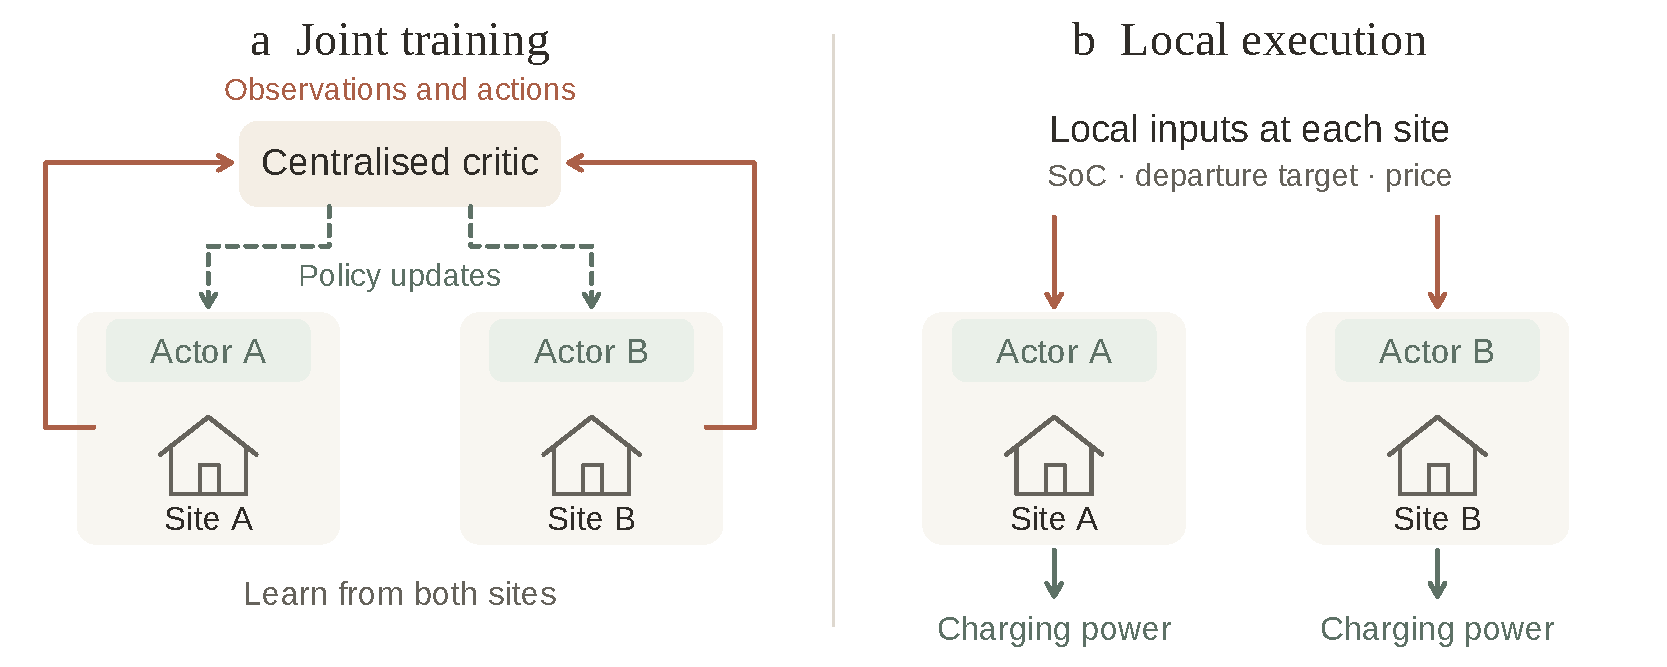
\includegraphics[width=\textwidth]{figures/foundations-ctde.pdf}
\caption{Centralised training and decentralised execution for two sites. Joint observations and actions support policy updates during training; local inputs determine charging decisions during execution. Original illustration based on \textcite{lowe2017maddpg}.}
\label{fig:ch2-ctde}
\end{figure}

\emph{Parameter sharing} allows several agents to use the same policy parameters. Two sites can apply the same charging rule to different \glspl{soc}, prices, and departure times, producing different actions from that common model. Their experience can jointly train the shared rule. The policy uses compatible input and action representations, with asset capabilities or roles included when needed \parencite{albrecht2024marl,yu2022mappo}.

Table~\ref{tab:ch2-learning-organisation} separates these three organisational choices. For example, sites can share policy parameters, train with joint information, and still choose their actions locally during operation.

\begin{table}[!tbp]
\centering\small
\caption{Three organisational choices in multi-agent learning and execution.}
\label{tab:ch2-learning-organisation}
\renewcommand{\arraystretch}{1.16}
\begin{tabularx}{\textwidth}{@{}>{\RaggedRight\arraybackslash}p{0.20\textwidth}>{\RaggedRight\arraybackslash}X>{\RaggedRight\arraybackslash}X@{}}
\toprule
\textbf{Dimension} & \textbf{Choices} & \textbf{\gls{rec}-related interpretation}\\\midrule
Learning information & Local information or information from several agents. & Updates use records from one site or combine observations and actions from several sites.\\\addlinespace[5pt]
Action selection & Centralised or decentralised execution. & One process selects all charging powers, or each site's agent selects its own.\\\addlinespace[5pt]
Policy parameters & Separate or shared parameters. & Agents use separate charging policies or apply the same model to their respective inputs.\\\bottomrule
\end{tabularx}
\end{table}

The next subsection examines how these learning and execution arrangements support coordinated charging, and how a shared outcome can provide useful feedback for the individual decisions that produced it.

\Needspace{7\baselineskip}
\subsection{Coordination and Credit Assignment}
\label{sec:ch2-credit}

The sites' separate charging choices combine into a \gls{rec} demand profile. \emph{Coordination} means that these choices account for their effects on the shared outcome. For example, agents can spread charging across the available low-price intervals while meeting departure targets, reducing the peak created when all vehicles charge together.

\emph{Credit assignment} concerns how a collective result informs the learning of individual agents. If the \gls{rec} peak falls, every agent may receive a better shared reward, although their charging decisions contributed differently to that reduction. Learning needs a way to relate the improvement to those individual choices.

\Needspace{9\baselineskip}
\emph{Counterfactual credit} evaluates one agent's alternatives while holding the other agents' actions fixed. A representative counterfactual baseline $b_i(s,a_{-i})$ is:
\begin{equation}
b_i(s,a_{-i})=
\mathbb E_{a_i'\sim\pi_i}
\left[Q(s,(a_i',a_{-i}))\right],
\label{eq:ch2-counterfactual-baseline}
\end{equation}
Here $a_{-i}$ contains all actions except agent $i$'s, and $Q$ evaluates a joint action in state $s$. The expectation averages over alternative actions $a_i'$ drawn from $\pi_i$, retaining the other agents' actions and the same local information. The difference between the selected joint action's value and this baseline gives agent $i$ an advantage signal \parencite{foerster2018coma}.

\emph{Value decomposition} relates individual utility estimates to a joint action value. Each utility provides a local score for an agent's action, and their combination estimates the collective return. When the combination is monotonic, increasing an individual utility cannot decrease the joint estimate. This property allows each agent to select its highest-scoring action consistently with maximising that estimate \parencite{rashid2018qmix}. In the \gls{rec} example, each site can select a charging action from its local scores while joint training relates their combination to the \gls{rec} outcome.

The next section turns from how agents learn together to the experience available for learning, explaining how policies can be trained from a fixed archive of recorded interactions through offline \gls{rl}.

\FloatBarrier
\section{Offline Reinforcement Learning}
\label{sec:ch2-offline}

The preceding sections described learning through interaction with an environment. \emph{Offline \gls{rl}} instead learns from a fixed dataset of interactions recorded before training begins \parencite{levine2020offline}. The thesis uses this setting to study learning from existing controller records; Section~\ref{sec:ch2-experience-literature} reviews the corresponding methods.

This dataset is an archive of past experience. Each recorded \emph{transition} links an observation or state to the action taken, its reward, and the next observation or state. For a charger, a record might associate the vehicle's \gls{soc} and departure time with the selected power, the charging cost, and the resulting \gls{soc}. Consecutive records can form a trajectory.

The learner repeatedly uses these records to estimate values or improve a policy, without collecting new interactions during training. Figure~\ref{fig:ch2-offline} separates data collection, learning from the fixed dataset, and subsequent use of the policy.

\begin{figure}[!htbp]
\centering
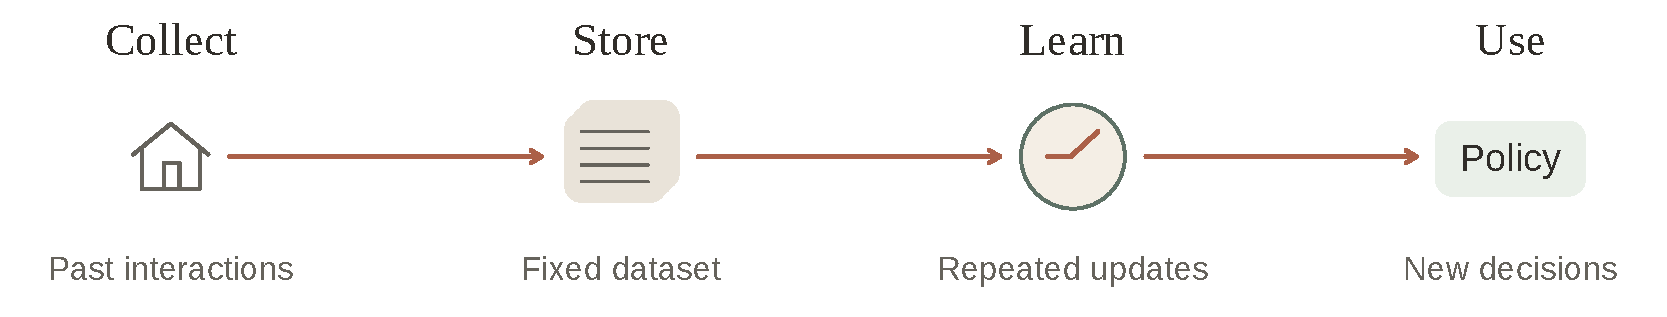
\includegraphics[width=\textwidth]{figures/foundations-offline.pdf}
\caption{Offline learning uses a fixed dataset collected beforehand. The trained policy subsequently receives new observations and selects actions.}
\label{fig:ch2-offline}
\end{figure}

\emph{Off-policy learning}, introduced in Section~\ref{sec:ch2-experience}, separates the policy being improved from the policy that generated the experience. A site can therefore learn from earlier charging decisions made by another controller while continuing to collect new interactions. Offline \gls{rl} uses this separation within a fixed dataset: the learner revisits the same records throughout training, and its updated policy is not used to obtain additional experience during that phase \parencite{levine2020offline}.

The usefulness of the archive depends on its coverage of conditions and decisions. Suppose that the recorded charging controller always starts at maximum power when an \gls{ev} arrives with a low \gls{soc}. Those records provide evidence about immediate charging in that condition, but little direct evidence about postponing it or selecting a lower power. Even a large archive can therefore leave some state--action combinations poorly represented. A new policy may select such combinations, and an inaccurate value estimate can make them appear more attractive than the recorded alternatives. Because offline training collects no additional interactions, the learner cannot test those choices and correct the estimate through new experience. This dependence on dataset coverage motivates the methods reviewed in Section~\ref{sec:ch3-data-prior-knowledge} \parencite{levine2020offline}.

\emph{\gls{bc}} treats each recorded action as a training target. Given the vehicle's condition, the model learns to reproduce the power selected by the collecting controller. Offline \gls{rl} instead uses the recorded rewards and transitions to learn about accumulated performance and improve the policy towards a return objective. Both approaches use past decisions, but their learning signals differ: cloning follows the demonstrated action, whereas offline \gls{rl} evaluates decisions through their recorded consequences.

This section established how recorded experience supports policy learning. The next section turns to how decisions are organised, introducing a hierarchy between \gls{rec} coordination and local control.

\Needspace{8\baselineskip}
\FloatBarrier
\section{Hierarchical Reinforcement Learning and Coordination}
\label{sec:ch2-hierarchy}

\gls{rec} coordination and local control concern different parts of the same charging process. A coordinator may guide when sites consume energy, while each site's controller selects the power requested from its chargers. A \emph{hierarchy} links these responsibilities by making local decisions depend on a higher-level choice. \gls{hrl} learns policies within this organisation. The following subsections explain the levels, timing, and signals used in the thesis, providing the foundations for understanding the methods reviewed in Section~\ref{sec:ch3-hierarchical-controllers}.

\Needspace{7\baselineskip}
\subsection{Decision Levels and Temporal Abstraction}
\label{sec:ch2-temporal-abstraction}

Section~\ref{sec:ch2-community-structure} organised the energy system into assets, sites, and \glspl{rec}, each with its own scope of operation. A control hierarchy assigns decisions across such scopes. In the running example, the \gls{rec} level supplies a coordination signal, and the site level uses that signal alongside its vehicles' requirements to choose charging powers. These responsibilities define the decision levels considered here.

The timing of a decision follows its role in this organisation. A coordinator might update its signal hourly while sites choose charging power every fifteen minutes, making four local decisions under the same signal. The levels can also share a decision interval while retaining different responsibilities.

\emph{Temporal abstraction} groups several elementary steps into one extended behaviour. In the \emph{options} framework, an option has an initiation set describing when it can begin, an internal policy selecting its actions, and a termination rule \parencite{sutton1999options}. A charging option might start when a vehicle connects and end when an energy target is reached or the vehicle departs.

\Needspace{7\baselineskip}
For an option lasting $\tau$ steps, the discounted accumulated reward $R_t^{(\tau)}$ is:
\begin{equation}
R_t^{(\tau)}=\sum_{k=0}^{\tau-1}\gamma^k r_{t+k}.
\label{eq:ch2-option-reward}
\end{equation}
Here $t$ is the starting step, $k$ counts steps within the option, $r_{t+k}$ is the reward following that step's action, and $\gamma$ discounts later rewards. Subsequent value is discounted by $\gamma^\tau$. Variable option durations give the higher-level process a semi-Markov formulation \parencite{sutton1999options}.

These levels and intervals specify when decisions occur. The next subsection explains what the higher-level choice communicates to a local policy.

\Needspace{7\baselineskip}
\subsection{Goals, Skills, and Coordination Signals}
\label{sec:ch2-hierarchy-signals}

A \emph{goal} describes the condition that a local controller should reach. For example, the higher level may assign an amount of energy to deliver before departure. The local policy then determines how charging power develops over the available intervals to pursue that target.

\Needspace{5\baselineskip}
A \emph{skill} provides a policy for a particular behaviour, such as charging steadily or adjusting charging to local generation. Selecting a skill delegates the subsequent power choices to that policy, which responds to the observations it receives. The higher level therefore selects a behaviour whose individual actions are determined locally \parencite{vezhnevets2017fun,nachum2018hiro}.

A \emph{power budget} specifies how much capacity a site can use for a given purpose during an interval. If two chargers share a 6~kW charging budget, the site controller can distribute that power between them according to their remaining energy needs and departure times. The budget sets the combined allowance while leaving the individual allocations to local control.

An \emph{incentive signal}, such as a price multiplier, influences how the local controller assesses possible schedules. A signal that makes the current interval less costly can favour charging during that interval. The resulting power request still follows from the site's conditions, including whether a vehicle is connected and how much energy it requires.

\Needspace{8\baselineskip}
A coordinator policy $\pi_{\mathrm H}$ can select a signal $g_k$ at time $t_k$, which then conditions the local policy $\pi_i$:
\begin{equation}
g_k\sim\pi_{\mathrm H}(\,\cdot\mid o^{\mathrm H}_{t_k}),
\qquad
a_{i,t}\sim\pi_i(\,\cdot\mid h_{i,t},g_k),
\quad t_k\leq t<t_{k+1}.
\label{eq:ch2-hierarchy-policies}
\end{equation}
Here $o^{\mathrm H}_{t_k}$ is the coordinator's observation, $h_{i,t}$ is agent $i$'s local information history, and $a_{i,t}$ is its action. The symbol $\sim$ denotes sampling, and the dot stands for the possible signal or action. The signal remains in use until the next coordinator decision at $t_{k+1}$.

The same incentive can produce different actions. A site with an unmet charging requirement may request power, while another with a fully charged vehicle selects zero. Figure~\ref{fig:ch2-hierarchy} connects these local responses to the shared signal and its update interval.

\begin{figure}[!htbp]
\centering
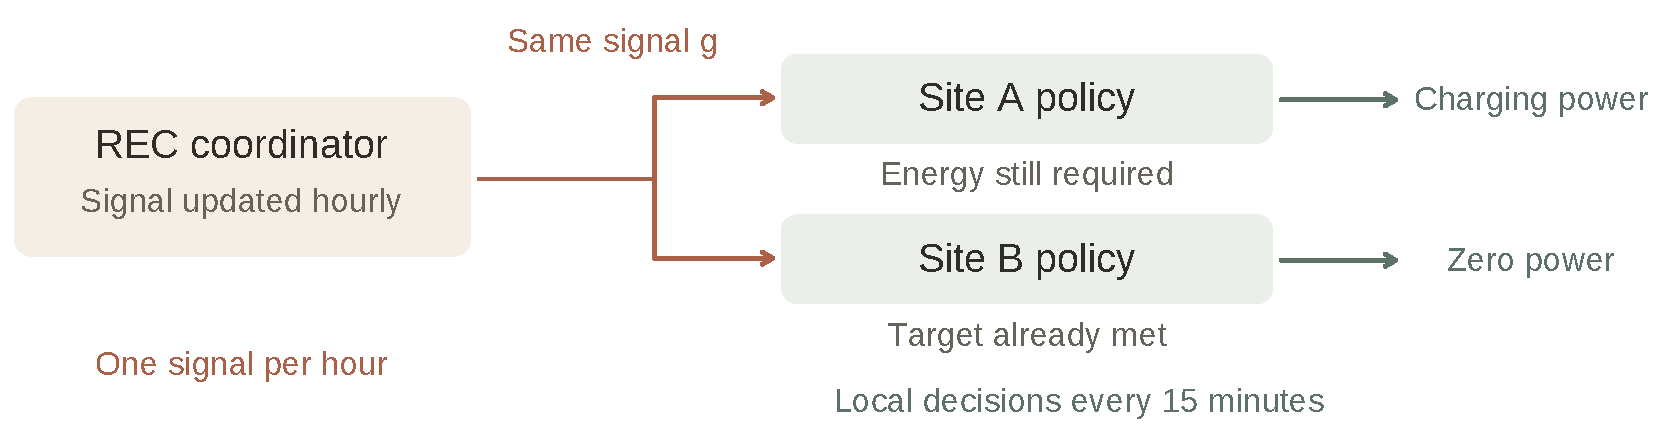
\includegraphics[width=\textwidth]{figures/foundations-hierarchy.pdf}
\caption{One \gls{rec} signal guides successive local decisions. Each site combines it with its own charging conditions to select a power request.}
\label{fig:ch2-hierarchy}
\end{figure}

Hierarchy establishes how decisions are distributed across levels. The next section examines the computation within each policy, from resource observations to the actions returned to individual assets.

\Needspace{8\baselineskip}
\FloatBarrier
\section{Structured Policy Architectures}
\label{sec:ch2-structured}

Section~\ref{sec:ch2-neural} introduced networks that transform numerical inputs into learned representations and outputs. Energy control also gives those quantities a physical organisation, with observations and actions belonging to particular sites and assets. This section develops the entity representations, attention mechanisms, and modular outputs needed to understand the architectures reviewed in Chapter~\ref{chap:related-work} and the method formulations developed in Chapters~\ref{chap:control-benchmark} and~\ref{chap:ti-marl}.

\Needspace{7\baselineskip}
\subsection{Entity and Relational Representations}
\label{sec:ch2-entities}

The numerical inputs introduced in Section~\ref{sec:ch2-neural} must describe the resources whose operation is being controlled. When a site contains several assets, their observations need an arrangement that preserves what each value refers to. A fixed observation vector provides one such arrangement by assigning a declared position to each feature.

For a site with a battery and two chargers, one group of positions can describe the battery and two further groups the vehicles connected to the chargers. The network receives the values in that order. Updating a vehicle's \gls{soc} changes a value; adding a third charger's observations changes the vector's length. The following representations organise these inputs around the resources themselves.

An \emph{entity representation} groups attributes around the resource they describe. Let $x_j$ contain the attributes of entity $j$. An encoder can map each $x_j$ into an embedding, using the same parameters for entities with a common attribute format. Two chargers can therefore use the same encoder while producing different embeddings from their respective \glspl{soc} and departure requirements. The number of entities and the number of attributes describing each entity are separate dimensions.

\Needspace{8\baselineskip}
A \emph{set representation} treats the entities as an unordered collection. One construction uses a shared encoder $\phi$ and an aggregation to produce a site representation $z$:
\begin{equation}
z=\rho\!\left(\sum_{j=1}^{m}\phi(x_j)\right),
\label{eq:ch2-set-representation}
\end{equation}
where $m$ is the number of entities, $\phi(x_j)$ is the embedding of entity $j$, and $\rho$ transforms the sum into the site representation \parencite{zaheer2017deepsets}. Each embedding has a common width, so the sum retains that width as $m$ changes. Adding a compatible charger introduces another application of the encoder and another term in the sum, using the same learned functions.

Reordering the elements leaves this sum unchanged. This property is \emph{permutation invariance}. A site-level value estimate, for example, can describe the same collection whether charger C1 is listed before or after charger C2. The ordering of the records does not change which physical resources are represented.

Resource-specific outputs use the complementary property of \emph{permutation equivariance}. When the input entities are reordered, their corresponding outputs follow the same reordering. If the policy returns one power request per charger, the request for C1 remains associated with C1 after the list order changes. A model can preserve each entity's embedding alongside an aggregate site context to retain this association.

A \emph{graph representation} additionally describes relationships between entities. Nodes can represent a battery, chargers, and their connection point; edges can indicate which assets share that connection. \emph{Message passing} updates a node's representation using information from its neighbours through shared transformations \parencite{gilmer2017mpnn}. In the site example, the connection node can collect information about the assets that draw on its capacity. Figure~\ref{fig:ch2-representations} shows the same resources as a vector, a set, and a graph.

\begin{figure}[!htbp]
\centering
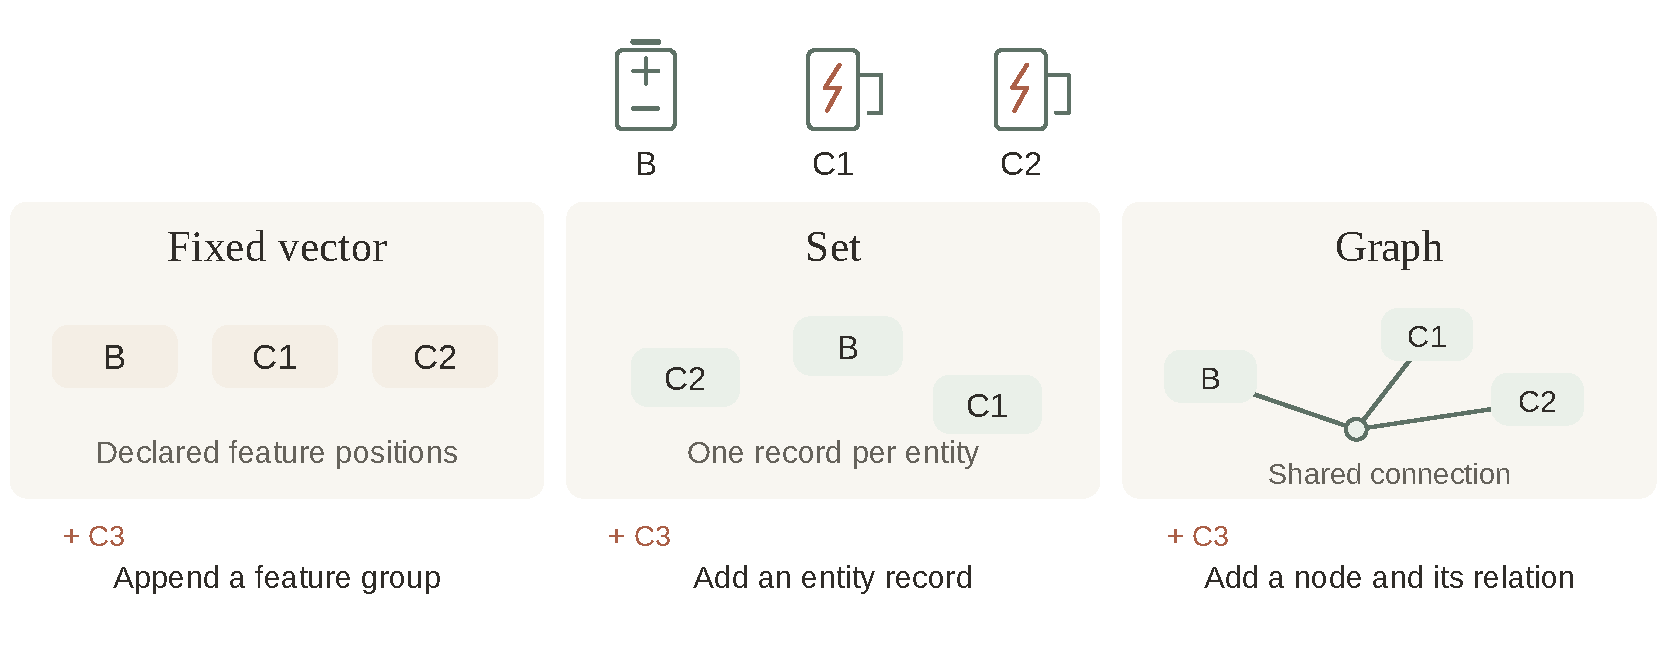
\includegraphics[width=\textwidth]{figures/foundations-representations.pdf}
\caption{Three representations of the same site resources. Vector positions identify feature groups, a set groups attributes by entity, and a graph includes declared relationships. The lower row illustrates adding another charger record.}
\label{fig:ch2-representations}
\end{figure}

\emph{Padding} fills unused positions when several collections are stored in an array with a common allocated size. A presence mask identifies which positions contain entities and which are padding. For example, a batch can allocate four charger positions per site while a mask marks the two populated positions at a particular site. The allocated length, the active entity count, and the embedding width describe different aspects of that representation.

These representations establish which elements enter the policy and how they are associated with resources. The next subsection introduces attention, explaining how the representation of one element can incorporate information from others before decisions are produced.

\Needspace{7\baselineskip}
\subsection{Attention and Transformer Architectures}
\label{sec:ch2-attention}

An entity's decision can depend on information elsewhere in the site. A charger's remaining energy requirement, for example, can be considered alongside another charger's deadline and the available connection capacity. \emph{Attention} forms a weighted combination of input representations, with the weights computed from learned comparisons between them \parencite{vaswani2017attention}.

The computation uses three projections of the available embeddings. A \emph{query} participates in the comparison for the element being updated, while each \emph{key} participates in the comparison for an element whose information may be used. The associated \emph{value} contains the information to combine. For a charger query, matching it against keys from the site produces weights for the corresponding value vectors.

\Needspace{8\baselineskip}
Scaled dot-product attention operates on query, key, and value matrices $Q$, $K$, and $V$:
\begin{equation}
\operatorname{Attention}(Q,K,V)
=\operatorname{softmax}\!\left(\frac{QK^{\mathsf T}}{\sqrt{d_k}}+M\right)V,
\label{eq:ch2-attention}
\end{equation}
where rows of $Q$ contain query vectors, rows of $K$ contain key vectors, and rows of $V$ contain their associated value vectors. The query and key width is $d_k$, and $\mathsf T$ denotes transposition. The optional additive mask $M$ is zero for permitted entries and negative infinity for excluded entries.

The query and key dot products form comparison scores, scaled by $\sqrt{d_k}$. The row-wise softmax turns each query's scores into non-negative weights summing to one over the permitted keys. Multiplication by $V$ then produces one weighted value combination for each query \parencite{vaswani2017attention}.

In \emph{self-attention}, the queries, keys, and values are projected from the same collection. Each site entity can thus receive information from other entities. In \emph{cross-attention}, the queries come from one collection and the keys and values from another. For example, queries associated with requested charging outputs can retrieve information from a collection of observation embeddings.

The number of rows and the width of each row play different roles. In self-attention over $m$ entities, the query and key matrices each have $m$ rows, while their projection widths are architectural choices. Changing $m$ changes the number of comparisons and output representations. A later aggregation can produce a single site representation, or subsequent computation can retain one representation per entity \parencite{lee2019settransformer}.

\emph{Multi-head attention} performs several attention computations using separate learned projections. Their results are concatenated and projected into the output representation. Each head supplies its own combination of values. In the running example, the combined representation draws on several learned comparisons among the same site entities.

A \emph{Transformer block} integrates attention with a feed-forward transformation applied to each element. The feed-forward part transforms the features within an element's representation after attention has combined information across elements. Stacking blocks repeats these operations, producing successive representations of the collection \parencite{vaswani2017attention}.

\emph{Residual connections} add a sublayer's input to its transformed output, retaining a direct path for the incoming representation. \emph{Layer normalisation} normalises features within each element and applies learned scale and offset parameters. Figure~\ref{fig:ch2-attention} relates an attention head to a Transformer block using residual addition and normalisation after each sublayer.

\begin{figure}[!htbp]
\centering
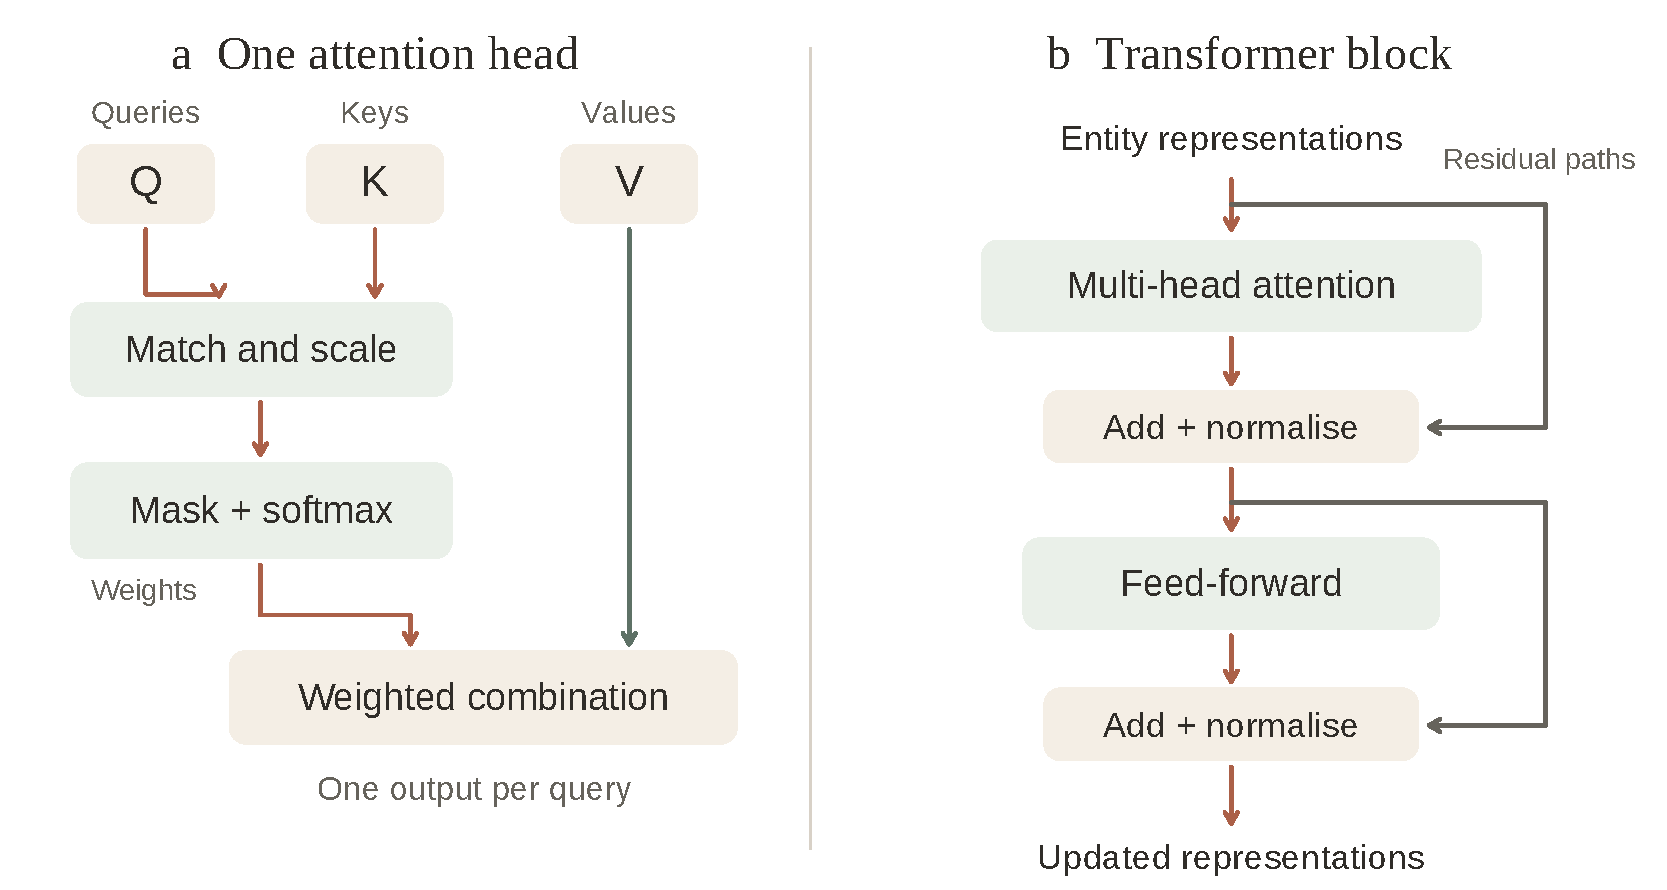
\includegraphics[width=\textwidth]{figures/foundations-attention.pdf}
\caption{Attention and a Transformer block. An attention head computes weights and combines values. Multiple heads form the attention sublayer of the illustrated block; residual paths feed the additions before layer normalisation. Original illustration based on \textcite{vaswani2017attention}.}
\label{fig:ch2-attention}
\end{figure}

Attention and Transformer blocks produce representations that combine the selected information. The next subsection explains how a policy organises those computations into modules and maps their outputs to actions with defined meanings for individual resources.

\Needspace{7\baselineskip}
\subsection{Modular Policies and Action Decoding}
\label{sec:ch2-modular-policies}

A \emph{modular policy} divides its computation into components with specified input or output roles. An encoder can prepare observations, a shared component can combine their representations, and a decoder can produce the quantities used to select an action. Components may be specialised for different resource types or reused across several instances of the same type \parencite{huang2020smp,luketina2025compositional}.

An \emph{output head} maps a representation into a particular group of outputs. A fixed head for two chargers can produce a two-component vector with one power request in each declared position. The number and meaning of those positions belong to the head's specification. This is the output-side counterpart of the fixed feature vector introduced in Section~\ref{sec:ch2-neural}.

A shared resource decoder applies the same function to each resource representation. For three compatible chargers, it produces three outputs, each associated with its source charger. Each evaluation has a fixed output width, while the number of evaluations follows the charger count. Figure~\ref{fig:ch2-modular} illustrates this reuse alongside a separate decoder for another action type.

\begin{figure}[!htbp]
\centering
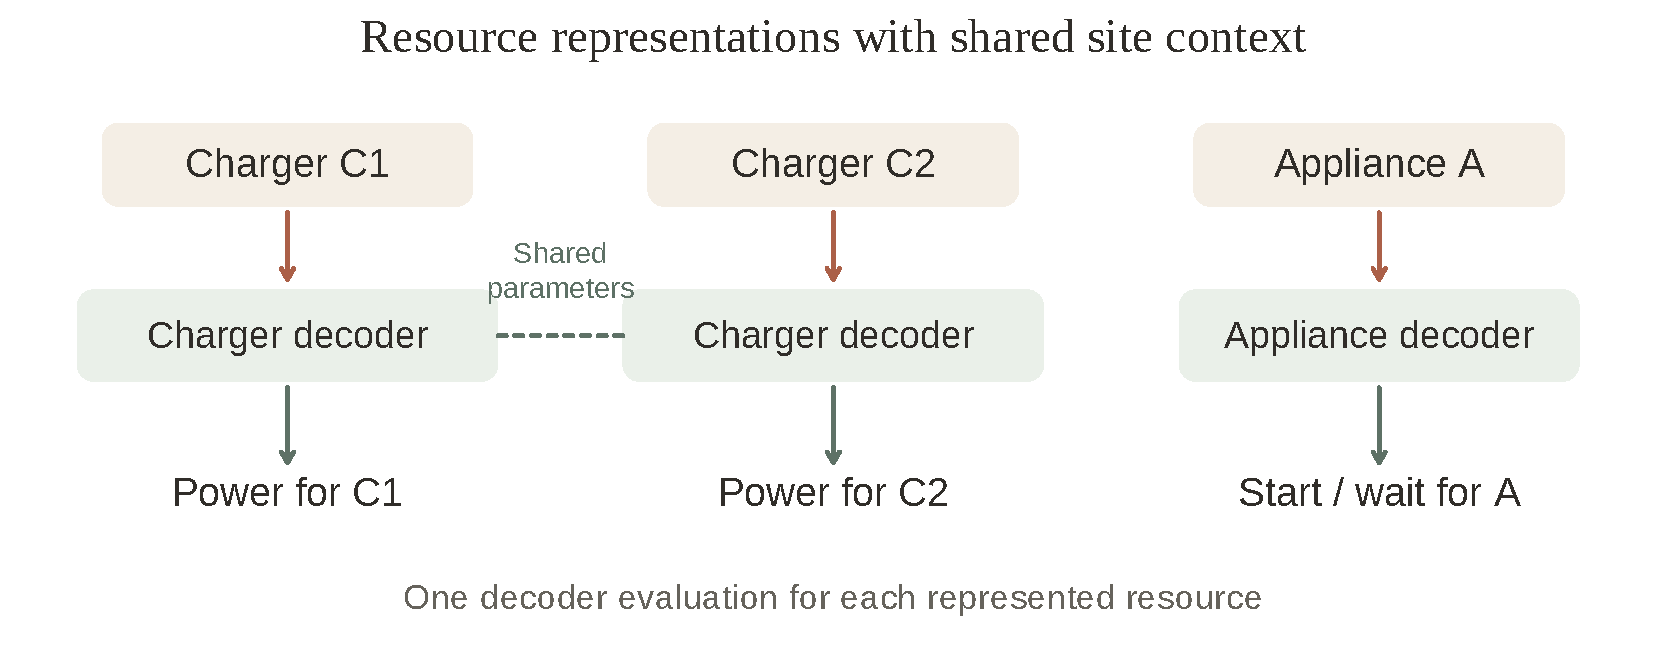
\includegraphics[width=\textwidth]{figures/foundations-modular.pdf}
\caption{Shared decoding with resource-specific outputs. The same charger decoder processes the representations of C1 and C2, producing a separate power request for each. A different decoder produces the appliance's discrete choice. Repeated decoder symbols denote shared parameters.}
\label{fig:ch2-modular}
\end{figure}

A \emph{parameterised action} combines a discrete choice with numerical parameters \parencite{li2022hyar}. A charger might select idle, charge, or discharge, with a power magnitude attached to an active mode. The decoder associates the mode and magnitude with the charger, while conversion to a physical request establishes its units and permitted range.

Resource count and resource type also describe different changes. Adding another charger with the same observation and action format adds another instance of the existing computation. Introducing an asset with a different sensor description or command family changes the input or output mapping required by that type. Type-specific encoders and decoders declare those mappings, while the resource association identifies which instance supplies or receives each quantity.

Structural compatibility concerns whether the architecture can process observations and produce actions for a changed configuration. Control generalisation concerns decision quality and any further learning needed, while computational scalability concerns time and memory requirements as resources increase. A shared decoder can serve a third compatible charger, but its vehicle adds a service request competing for connection capacity. The resulting schedule and additional processing must therefore be assessed. Section~\ref{sec:ch3-scalability} examines these distinctions through the capabilities and evaluation conditions reported in the literature.

The representations, information exchange, and output mappings described here complete the architectural foundations used in the thesis. The chapter summary brings them together with the energy and learning concepts before the next chapter examines the methods built from them.

\FloatBarrier
\section{Chapter Summary}
\label{sec:ch2-summary}

This chapter presented the energy and learning concepts needed to follow the controller formulations developed in the thesis. It began by distinguishing the members of a \gls{rec}, the sites where energy is used, and the assets whose operation can be controlled. Flexibility described the adjustments available within physical limits and service requirements. The charging example illustrated how those adjustments depended on the vehicle's energy needs, connection period, and operating conditions.

Neural networks provided the computational basis for mapping observations to predictions or decisions. The chapter explained how numerical inputs pass through learned intermediate representations to produce outputs, distinguishing changes in input values from changes in the number of components expected by a dense network. These distinctions prepared the later discussion of resource representations.

\gls{rl} placed those decisions within a sequence of actions and consequences. Rewards expressed the objective, returns combined rewards over time, and value functions assessed the expected consequences of following a policy. \gls{marl} extended this account to several interacting agents. In the \gls{rec} example, individually selected charging powers combined into a shared demand profile, connecting local decisions with the need for coordination.

Offline \gls{rl} explained how a policy could be learned from a fixed collection of recorded interactions. Hierarchical control then organised decisions across responsibilities and time scales, with a \gls{rec}-level choice guiding local controllers. The same signal could produce different charging powers because each site also acted on its own vehicle requirements.

Structured policy architectures connected these decision mechanisms to the resources being represented and controlled. Entity-based inputs preserved the association between observations and assets, attention combined information across resources, and shared decoders produced actions for individual instances. The chapter distinguished adding another compatible resource from introducing a new resource type, establishing the concepts needed to discuss changes in a policy's inputs and outputs.

The chapter did not examine the detailed foundations of data acquisition and preparation, state estimation, flexibility prediction, or demand and generation forecasting, because its scope was the learning and decision mechanisms used for \gls{rec} energy control. These subjects remain necessary for other parts of the project, including supplying controller inputs and constructing the experimental setting. Keeping their detailed treatment separate allowed the chapter to follow a continuous path from the energy problem to the formulation of learned decisions.

Chapter~\ref{chap:related-work} now examines how existing methods use these foundations to control energy resources and identifies the gaps that underpin the research problems introduced in Chapter~\ref{chap:introduction}.

\clearpage
\endgroup

\chapter{An Architecture for Real-World Community Energy Control: EnergAIze}
\label{chap:energAIze}
\label{chap:lifecycle}
\markboth{An Architecture for Real-World Community Energy Control}{An Architecture for Real-World Community Energy Control}
\newlength{\architectureoriginalparskip}
\setlength{\architectureoriginalparskip}{\parskip}
\setlength{\parskip}{0pt}
\newlength{\architectureoriginaltextfloatsep}
\newlength{\architectureoriginalintextsep}
\newlength{\architectureoriginalcaptionskip}
\setlength{\architectureoriginaltextfloatsep}{\textfloatsep}
\setlength{\architectureoriginalintextsep}{\intextsep}
\setlength{\architectureoriginalcaptionskip}{\abovecaptionskip}
\setlength{\textfloatsep}{12pt plus 2pt minus 2pt}
\setlength{\intextsep}{12pt plus 2pt minus 2pt}
\setlength{\abovecaptionskip}{6pt}
\raggedbottom
\edef\architectureoriginalclubpenalty{\the\clubpenalty}
\edef\architectureoriginalwidowpenalty{\the\widowpenalty}
\clubpenalty=10000
\widowpenalty=10000

The preceding chapter reviewed approaches to \gls{rec} energy control and identified gaps in their use in real-world installations. This chapter presents the architecture of EnergAIze, connecting control in buildings and \glspl{rec} to controller development, experiment orchestration, and deployment.

\section{Energy Control in Buildings and Communities}
\label{sec:energAIze-overview}
\label{sec:energaize-overview}
\label{sec:energAIze-functional-view}
\label{sec:energaize-community-view}

Households need their vehicles ready for travel, their rooms at a comfortable temperature, and their appliances to complete their work. Meeting these needs leaves choices about when electricity is consumed or stored, especially where a building also produces some of its own energy. To make those choices, a controller needs information about the services people require, the resources available to deliver them, and the limits within which they can operate. EnergAIze connects this information to the equipment through which a decision takes effect.

Consider the vehicle introduced in Chapter~\ref{chap:introduction}, arriving home at 18:00 with a \gls{soc} of 30\% and a target of 80\% by 08:00. The charger reports that the vehicle is connected, vehicle information supplies its \gls{soc}, and the household meter shows how much power the other loads are using. Together with the departure requirement and the available charging capacity, these observations allow the controller to choose a charging power. That decision is sent through the installation's control interface, and subsequent measurements report the power delivered and the progress towards the target.

\Cref{fig:energaize-building-loop} presents this flow. In the figure, \emph{State of the Environment} denotes the observations assembled for a decision. EnergAIze uses them to determine actions for the connected resources. Measurements and actions pass through the local control system or external service provider associated with the equipment.

\begin{figure}[htbp]
\centering
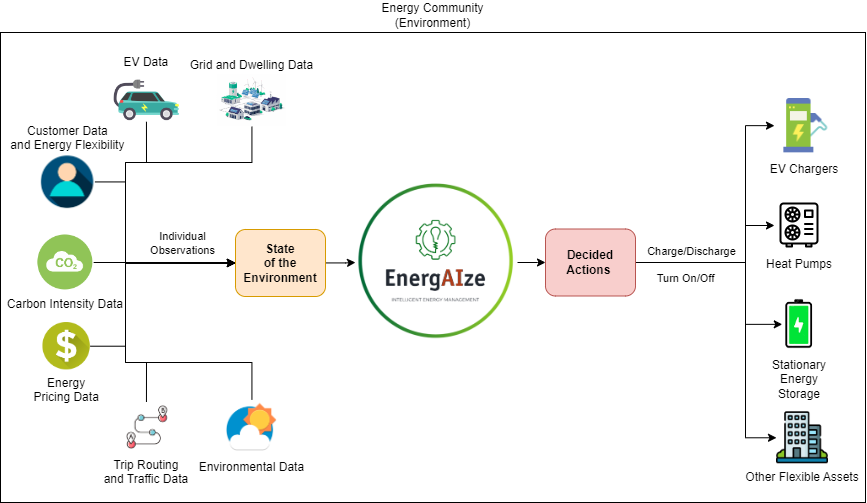
\includegraphics[width=\linewidth]{energaize-information-actions.png}
\caption[Information and actions in EnergAIze.]{Information and action flow. Source: author's master's dissertation.}
\label{fig:energaize-building-loop}
\end{figure}

The inputs shown in \cref{fig:energaize-building-loop} fall into seven categories, according to the information they contribute to a decision:

\begin{description}[font=\normalfont\bfseries,leftmargin=0pt,itemsep=0.25\baselineskip,topsep=0.4\baselineskip]
\item[User requirements and flexibility.] Requested services and the freedom to adjust their delivery, such as a vehicle's departure time and target \gls{soc}, a comfort range, or an appliance's operating window.
\item[Vehicle data.] Battery \gls{soc}, charging status, and battery capacity. These describe the vehicle's current condition and help determine the energy needed for its next use.
\item[Building and grid data.] Demand, \gls{pv} production, storage state, grid exchange, and connection limits. These describe the installation's energy balance and the capacity available for flexible resources.
\item[Electricity prices.] Purchase prices and, where applicable, export remuneration or \gls{rec} exchange prices. Their variation over time informs the cost of a charging or storage decision.
\item[Carbon intensity.] Emissions associated with electricity supply. This information allows the controller to consider the emissions consequences of using grid electricity at different times.
\item[Environmental data.] Weather conditions and forecasts, including temperature and solar irradiance. These help anticipate changes in renewable production and weather-dependent demand.
\item[Travel and traffic data.] Planned journeys, routes, and traffic conditions. These can inform estimates of vehicle arrival, departure, and energy use, complementing the requirements supplied by the user.
\end{description}

These categories can contain measurements, user declarations, configuration values, or forecasts. The vehicle's current \gls{soc} is a measurement; its required departure charge is a user requirement; its expected return time may be a forecast. Keeping these roles distinct allows the controller to use each value appropriately. The input selection for each experiment is retained in the configuration records described in Appendix~\ref{app:controller-configurations}.

The loop repeats as conditions change. Cooking and heating can reduce the power available for charging; when those loads subside, charging can increase. At each decision interval, the controller receives updated measurements and accounts for the time remaining before departure. The measurements also show how closely the delivered power followed the request.

Across a \gls{rec}, this arrangement is repeated for buildings with different equipment and daily routines. One household may have \gls{pv} panels and a battery, another a vehicle charger, and a workplace several charging points. Each building has a controller and associated data processing, configured for its resources. Measurements and actions remain linked to that building, while information relevant to the \gls{rec} can be shared among the participating controllers.

\Cref{fig:energaize-community} extends the first view to several buildings. Each local controller receives observations from its building and returns actions to its equipment. In the illustrated deployment, a \gls{rec} server supplies shared information, including time, weather, carbon intensity, and electricity prices. The actor network represents the learned controller executed for each building. This organisation also accommodates the hierarchical methods developed in Chapter~\ref{chap:control-benchmark}, where a \gls{rec} controller supplies guidance for local decisions.

\begin{figure}[htbp]
\centering
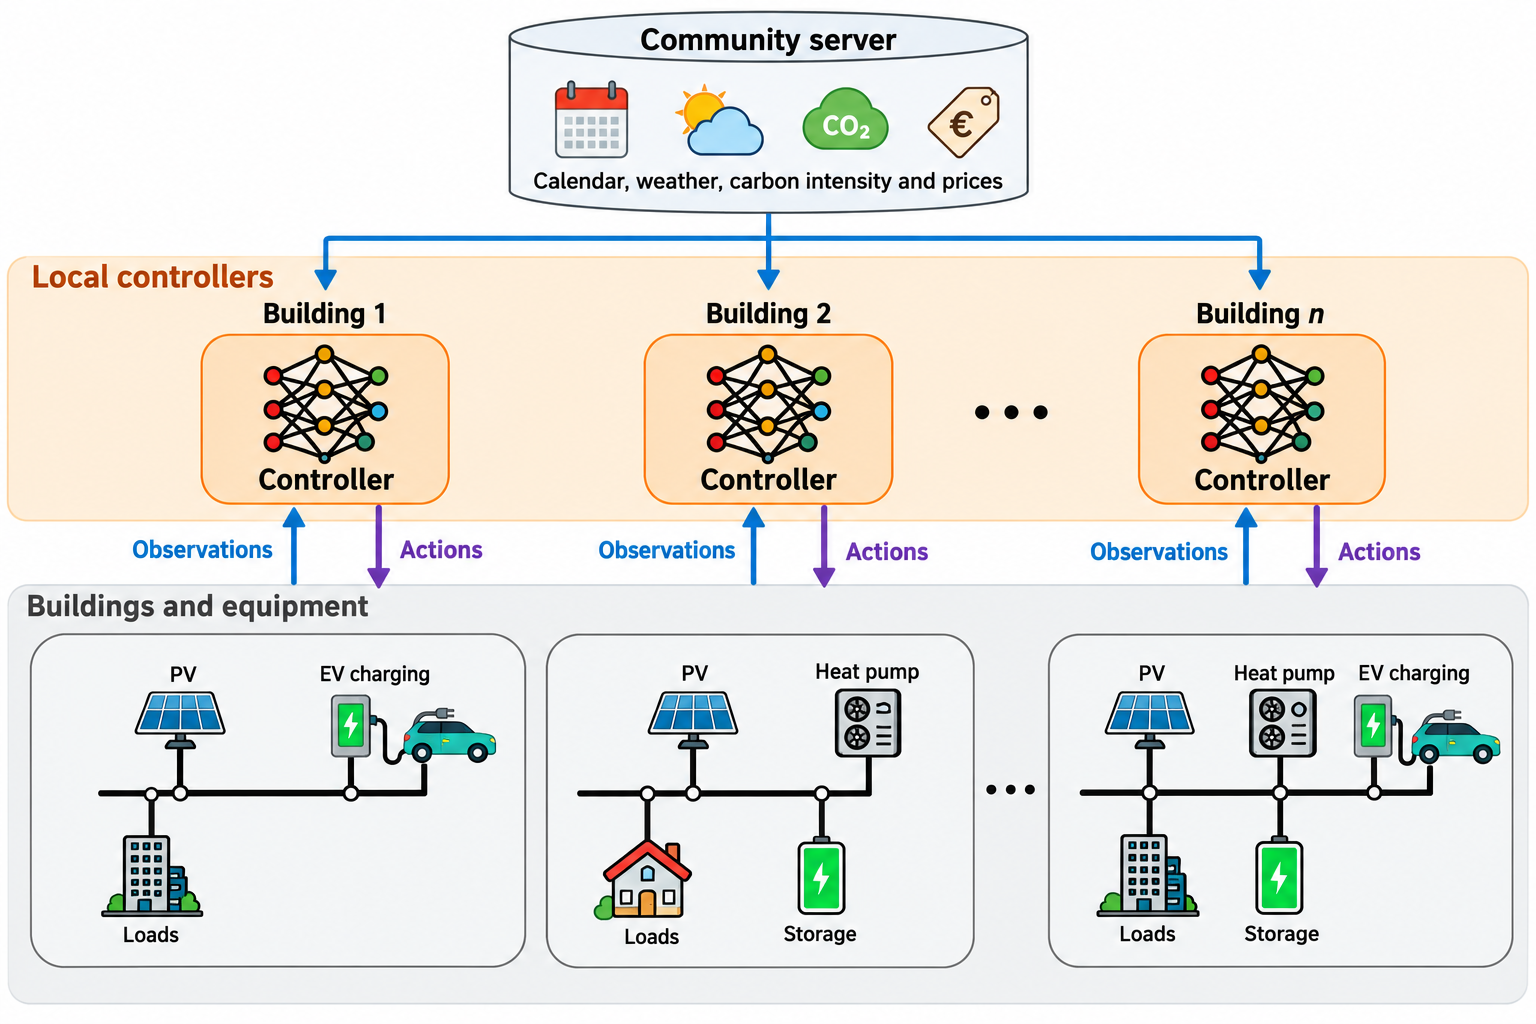
\includegraphics[width=\linewidth]{energaize-community-deployment-revised.png}
\caption[Building controllers within a \gls{rec}.]{\gls{rec} deployment. Adapted from the author's master's dissertation.}
\label{fig:energaize-community}
\end{figure}

\Needspace{3\baselineskip}
The blue arrows carry observations from each building and the shared services into its controller; the purple arrows carry the resulting actions to its equipment. For the charging example, local information establishes what the household can do, while \gls{rec} information helps determine when that flexibility is useful. On a different day, when the vehicle remains connected until late afternoon, the controller can account for renewable production available elsewhere in the \gls{rec}. When many vehicles arrive together, spreading charging over their connection windows can limit the combined demand.

Organising data processing and control around each building gives installation-specific work a clear scope. Connecting a new charger changes that building's configuration and available actions. Adding a building introduces another local loop and updates the \gls{rec} information used for coordination. Processing close to the data source can reduce communication and keep detailed measurements within the local processing path. The controllers in \cref{fig:energaize-community} coexist with shared services and provider platforms, with placement determined by each installation.

\begin{samepage}
Putting these local control loops into operation involves two complementary paths. During \emph{runtime}, incoming observations support a decision whose consequences are measured at the installation. During \emph{development}, data and simulation provide the conditions in which a controller is prepared and evaluated for that role. The runtime path is considered first, establishing what the controller must receive and produce. The development path then explains how such a controller is obtained, followed by the infrastructure that runs the experiments and loads the selected model into service.

\end{samepage}

% Keep the runtime overview in the chapter's portrait page orientation.
\section{Runtime Architecture}
\label{sec:energaize-runtime}

The information and action flow described above requires several services to work within each decision interval. Measurements must reach the controller in a usable form, the controller must choose an action, and that action must reach the equipment with the applicable checks. The \gls{cw} cloud platform and other \gls{iot} interfaces connect the equipment to these services through \glspl{api}. \Cref{fig:energaize-overview} shows how EnergAIze assigns these responsibilities, expanding one building to expose its runtime components.

\begin{figure}[H]
\centering
\makebox[\linewidth][c]{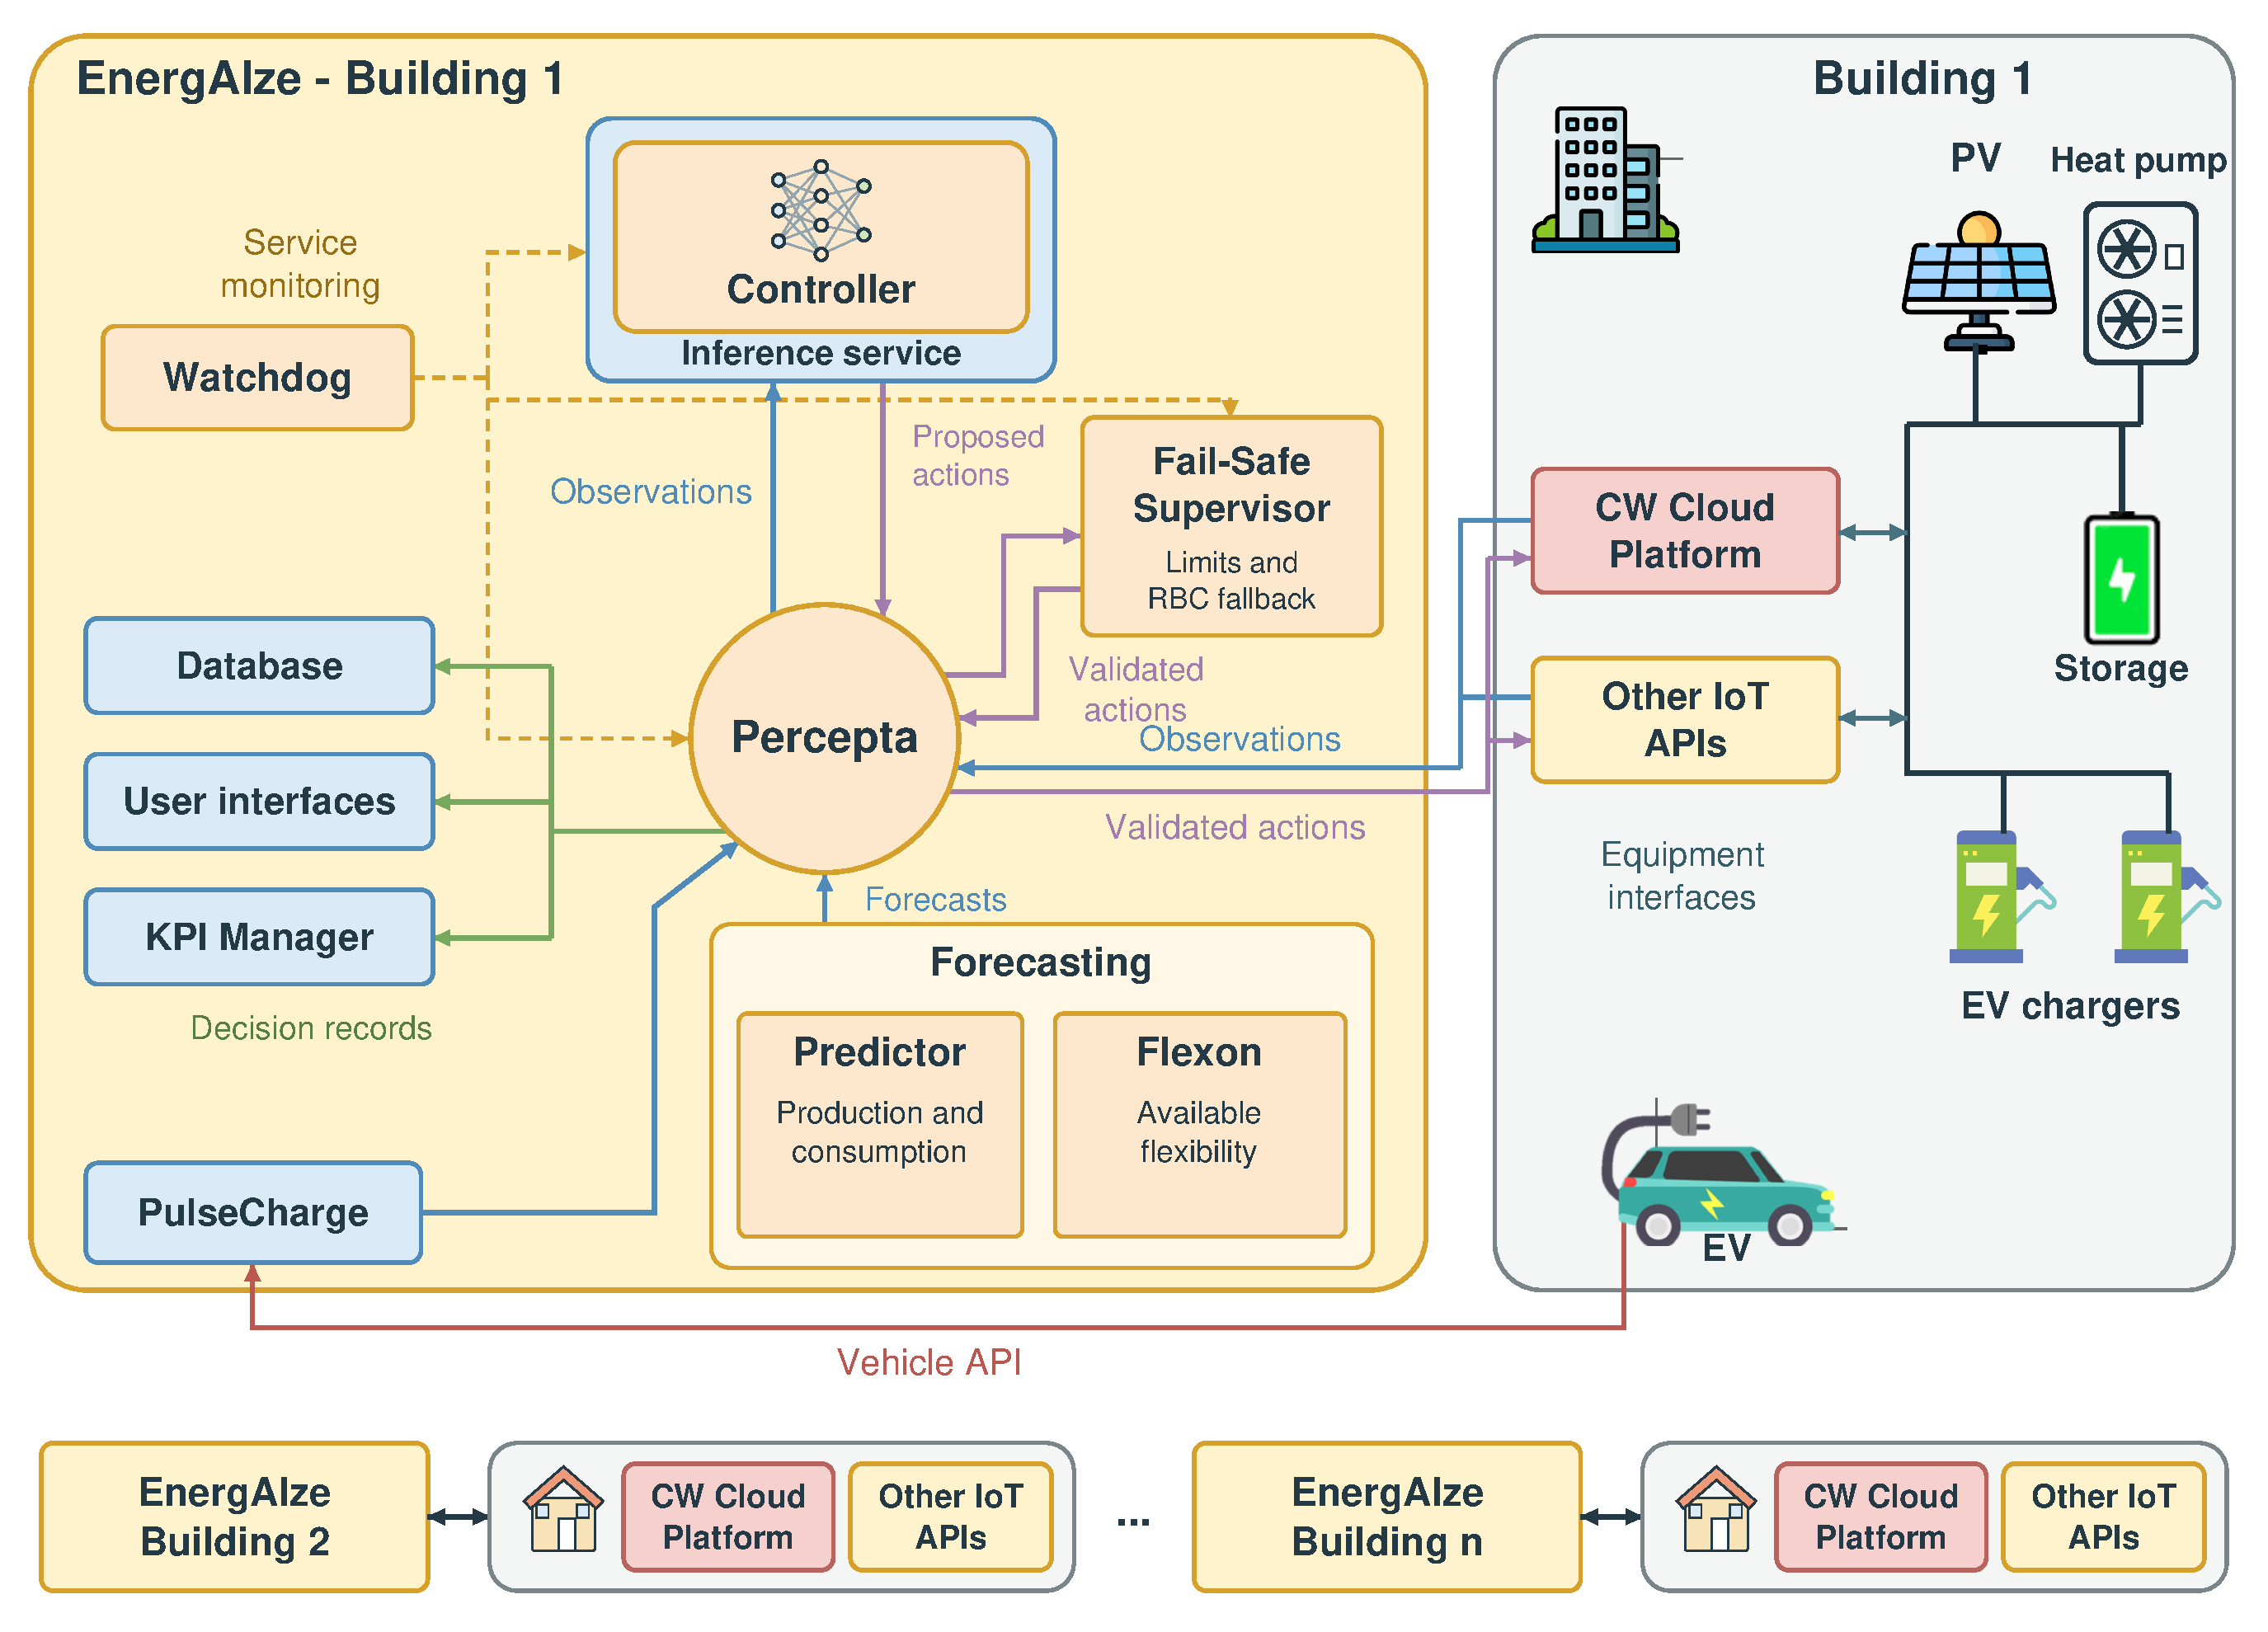
\includegraphics[width=1.1\linewidth]{energaize-runtime-revised.pdf}}
\caption[Runtime architecture of EnergAIze.]{Runtime architecture of EnergAIze, expanded for one building.}
\label{fig:energaize-overview}
\end{figure}

\begin{samepage}
On the right of the figure, the \gls{cw} cloud platform and other \gls{iot} interfaces connect the physical equipment to EnergAIze. On the left, Percepta processes incoming observations and routes outgoing actions. Vehicle information and forecasts support the controller, while action validation, service monitoring, and operational records accompany its decisions. This organisation underlies the integrations described in the EnergAIze publications and \gls{opeva} demonstrator \parencite{fonseca2024energAIze,fonseca2025realworldrec,opeva2026d63}.

\end{samepage}

\begin{samepage}
Installation configuration links these components to equipment, measurement sources, commands, and operating limits. A model contract specifies the controller's inputs and outputs; Section~\ref{sec:energaize-contract} describes its passage into runtime. The architecture and the roles of its components were conceived and designed by the author, who also guided the collaborative research and student projects through which several components were implemented. Their implementation contributions are acknowledged in the associated publications and the Statement on Co-Authored Work.

\end{samepage}

\subsection{The Controller and Its Inference Service}
\label{sec:energaize-algorithms}

At the centre of the runtime is the controller, shown within the inference service in \cref{fig:energaize-overview}. It determines how the resources under its control should operate during the next interval. The surrounding services supply information, apply its decisions, and report their consequences. The control methods investigated in Chapters~\ref{chap:control-benchmark} and~\ref{chap:ti-marl} occupy this position in the architecture.

For the household vehicle, the immediate choice is the charging power to request. Its consequences extend beyond the next interval: charging now contributes towards the departure requirement but also increases household demand, while delaying charging preserves capacity now and leaves less time to deliver the remaining energy. A stationary battery introduces a related choice. Discharging it may support the household during a busy period, although the energy then used will no longer be available later. The controller considers these resources together, using the observations and forecasts selected for its decision problem.

The control methods reviewed in Chapter~\ref{chap:related-work} can occupy this role through a common observation and action interface. A \gls{rbc} applies its configured rules, an optimisation method solves the current scheduling problem, and a learned controller evaluates its policy. The reinforcement-learning methods studied in this thesis use that interface during both development and operation, keeping decisions associated with the same resources and service requirements.

At \gls{rec} level, the decisions made in one building influence the conditions experienced by others. Several households postponing charging until the same low-price interval can create a new peak. Coordination requires the controller formulation to represent the relevant \gls{rec} information and relationships, whether through shared observations, the learning process, or guidance from a \gls{rec} controller. The runtime provides the communication and resource associations needed by the selected method. The progression from building decisions to coordinated and hierarchical control is developed in Chapter~\ref{chap:control-benchmark}; Chapter~\ref{chap:ti-marl} examines how the controller can accommodate changes in the participating resources.

The inference service executes the model selected for this role. It receives the prepared observations, applies the input processing declared by the model contract, evaluates the model, and returns named actions. The algorithm determines the decision; the service supplies the software interface through which that decision becomes available to the rest of EnergAIze. A compatible rule-based policy can occupy the same interface. Keeping the observation and action interpretation with the model allows a selected controller to be loaded without reconstructing its processing by hand.

The returned actions are proposals for the current interval. Before they reach the charger or battery, they pass through the validation and provider interfaces described below. Subsequent measurements close the loop by revealing what the equipment actually did. Preparing the inputs for this sequence begins with the data-integration service.

\subsection{Data Integration and Routing: Percepta}
\label{sec:energaize-percepta}

The measurements required for a decision can arrive through different interfaces and at different times. A building energy-management platform may expose meter readings and battery status, a charging platform may report connection and charging power, and a vehicle service may provide \gls{soc}. The stream-processing component, Percepta, handles the integration and processing of these sources so that the controller receives observations associated with the correct building and resources \parencite{percepta2025}.

Source-specific receivers obtain the incoming data, and translators map their fields into the representation used by the installation. Subsequent processing aligns the values used for a decision interval. For example, charging power reported in watts and household demand reported in kilowatts must be expressed consistently before they enter a common calculation. Their timestamps also matter: a charging measurement taken before the vehicle disconnected describes a different condition from the latest connection status. The data-processing path retains these associations when assembling the controller's observations.

In the \gls{opeva} integration, the Data Provider implements this path through receivers, translators, queues, an accumulator, and a manager that prepares the inference request \parencite{opeva2026d63}. The same integration work supports the retrieval of historical records for development. On the action path, a forwarder converts the validated action into the format and destination required by the equipment provider. This arrangement places provider-specific communication at the boundary of the system, allowing the controller to work with the observation and action names defined for the installation.

\subsection{Vehicle Information: PulseCharge}
\label{sec:energaize-pulsecharge}

Vehicle information extends what can be learned from the charger. The vehicle-data service, PulseCharge, retrieves information such as \gls{soc} and charging status through manufacturer interfaces, subject to the information available for the connected vehicle. It handles the corresponding authentication and periodic data retrieval, then makes that information available to the data-processing path.

In the running example, the charger establishes that a vehicle is connected, while PulseCharge can supply the 30\% \gls{soc} needed to determine how much energy remains to be delivered. These sources describe the same charging session from different points: one reports the charger and its power, the other the vehicle and its battery. Associating them with the correct vehicle and charger allows the controller to interpret them together. The charging platform remains the interface through which the charging action is applied.

\subsection{Production and Consumption Forecasting}
\label{sec:energaize-prediction}

The production and consumption forecasting services, represented by \emph{Predictor} within the forecasting group in \cref{fig:energaize-overview}, supply expected conditions over the period considered by the controller. Production forecasts estimate \gls{pv} output; consumption forecasts estimate the demand against which charging or battery operation will take place. Their inputs can include historical measurements, weather information, and calendar variables. Percepta makes the resulting forecasts available alongside the latest observations, with the forecast horizon and time interval identifying the period they describe.

For the vehicle arriving at 18:00, a forecast of high household demand can support spreading charging over the night. If the vehicle remains at home on another day, a forecast of substantial midday production may favour charging during that period. Each forecast concerns a future quantity whose realised value will later be measured. As new observations arrive, subsequent decisions can account for the difference between the expected and actual conditions. This connection keeps forecasts within the ordinary sequence of measurement, decision, and response.

\subsection{Flexibility Forecasting: Flexon}
\label{sec:energaize-flexon}

The flexibility-forecasting component, Flexon, estimates the flexibility expected to be available from participating resources. Within the forecasting role shown in the runtime figure, it supplies information about opportunities to adjust consumption or storage. For vehicle charging, this includes anticipating when a vehicle will be available and the energy associated with its expected use. The controller can then consider whether the anticipated connection window offers room to move charging towards a more favourable period.

User requirements establish the service to be delivered during the current connection. In the example, the driver requests 80\% by 08:00. If an earlier departure is specified, the available charging window becomes shorter even when previous journeys suggest a later departure. The controller receives both the forecast used to anticipate availability and the current requirement that its decisions must satisfy. Production and consumption forecasts describe the energy conditions around this opportunity; Flexon describes the flexibility expected to be available within it.

\subsection{Action Validation: Fail-Safe Supervisor}
\label{sec:energaize-supervision}

The Fail-Safe Supervisor is a separate component between the controller's proposed action and the request sent to the equipment. It checks the proposal against the installation's operating limits and current resource information, including charger ratings, battery limits, and available connection capacity. A proposal within those limits passes through unchanged; where a request exceeds the available capacity, the supervisor limits it before forwarding. In the \gls{opeva} middleware, validation precedes the forwarder that constructs the provider request \parencite{opeva2026d63}.

Each part of this path has a distinct responsibility. The controller's feasibility mechanisms account for the constraints represented by its method, while the inference service applies the output bounds and resolution declared for the model. The supervisor checks the resulting request against the operating conditions reported by the installation. Provider platforms and equipment retain their own protections when executing the validated action. This separation preserves the distinction between policy proposals, supervisory intervention, and equipment response developed in Section~\ref{sec:ch2-safety-literature}.

For the household vehicle, an increase in other loads may leave less power available than the controller requested. The supervisor reduces the charging command to the available capacity, and the next measurements show how much energy was delivered. Subsequent decisions then account for the energy still required before 08:00. The record of the original proposal and its correction makes it possible to examine both the immediate limit and the effect on departure readiness.

If the algorithm stops or produces no inference output for the current interval, the supervisor uses a lightweight \gls{rbc} to provide a fallback action. Its configured rules use the available operating information and remain subject to the installation's limits. The supervisor logs these fallback decisions as well as adjustments to policy proposals. The resulting records show when the learned controller supplied the action, when supervision changed it, and when control continued through the fallback.

\subsection{Service Monitoring: Watchdog}
\label{sec:energaize-watchdog}

The Watchdog monitors the services involved in the control loop, including data processing, controller execution, and supervision. It identifies interruptions so that the affected service can be examined and restored. The supervisor provides the immediate fallback when an inference output is unavailable; the Watchdog makes the service interruption visible to the operator. Its scope follows the dependencies: losing one vehicle-data source affects that vehicle's observations, while losing a shared inference service may affect several buildings. Resuming learned control requires the relevant observations and inference outputs to be available again.

Data availability also matters while the services themselves remain running. In the documented \gls{opeva} middleware, an absent measurement can be completed with the previous value when preparing an interval \parencite{opeva2026d63}. Its source time remains important when deciding how that value can be used. A delayed price update and an unavailable battery \gls{soc} have different implications for the charging decision. The response depends on the information needed for the requested action and the alternative control behaviour configured for the installation.

\subsection{Operational Records, User Interfaces, and KPI Manager}
\label{sec:energaize-records}

The database retains observations and decision records so that the course of operation can be examined. These records associate the controller version and its observations with the proposed action, any supervisory adjustment or fallback, the validated action, the provider response, and subsequent measurements. For the vehicle, they allow a reduction in charging power to be traced to the policy, the supervisor, or the equipment. Keeping that distinction through the session connects each intervention to the energy delivered before departure.

The graphical user interfaces give operators access to the current state of the installation and its operational records. They provide a way to inspect the participating resources, follow their measurements and actions, and examine interruptions reported through monitoring. An operator investigating unexpectedly slow charging can therefore relate the requested power to the vehicle state and the limits applied along the control path.

The \gls{kpi} Manager calculates \glspl{kpi} from the recorded operation. Electricity cost and peak demand can be examined at building and \gls{rec} level, alongside the vehicle's \gls{soc} at departure. The intervention records show when those outcomes were obtained with corrections or fallback control. The same operational records supply data and cases for subsequent training and evaluation.

\section{Controller Development}
\label{sec:energaize-development-runtime}
\label{sec:lifecycle-architecture}

The runtime architecture establishes what a controller receives, how its proposals reach the equipment, and how their consequences are recorded. Development prepares the controller for that role. Historical data and installation configuration provide the starting point, while simulation allows candidate policies to encounter successive conditions and be evaluated against the services they should deliver. The same process supports later retraining when operational records reveal conditions that call for a revised controller.

\Cref{fig:energaize-development} follows this controller through development. Installation records~(1) and \gls{rec} configuration~(2) define the scenarios~(3). Training~(4) and evaluation~(5) lead to the selected model bundle~(6), which reappears at the start of the deployment view in \cref{fig:energaize-deployment}. The computing infrastructure in Section~\ref{sec:orchestration} executes the training and evaluation stages as experiments.

\begin{figure}[htbp]
\centering
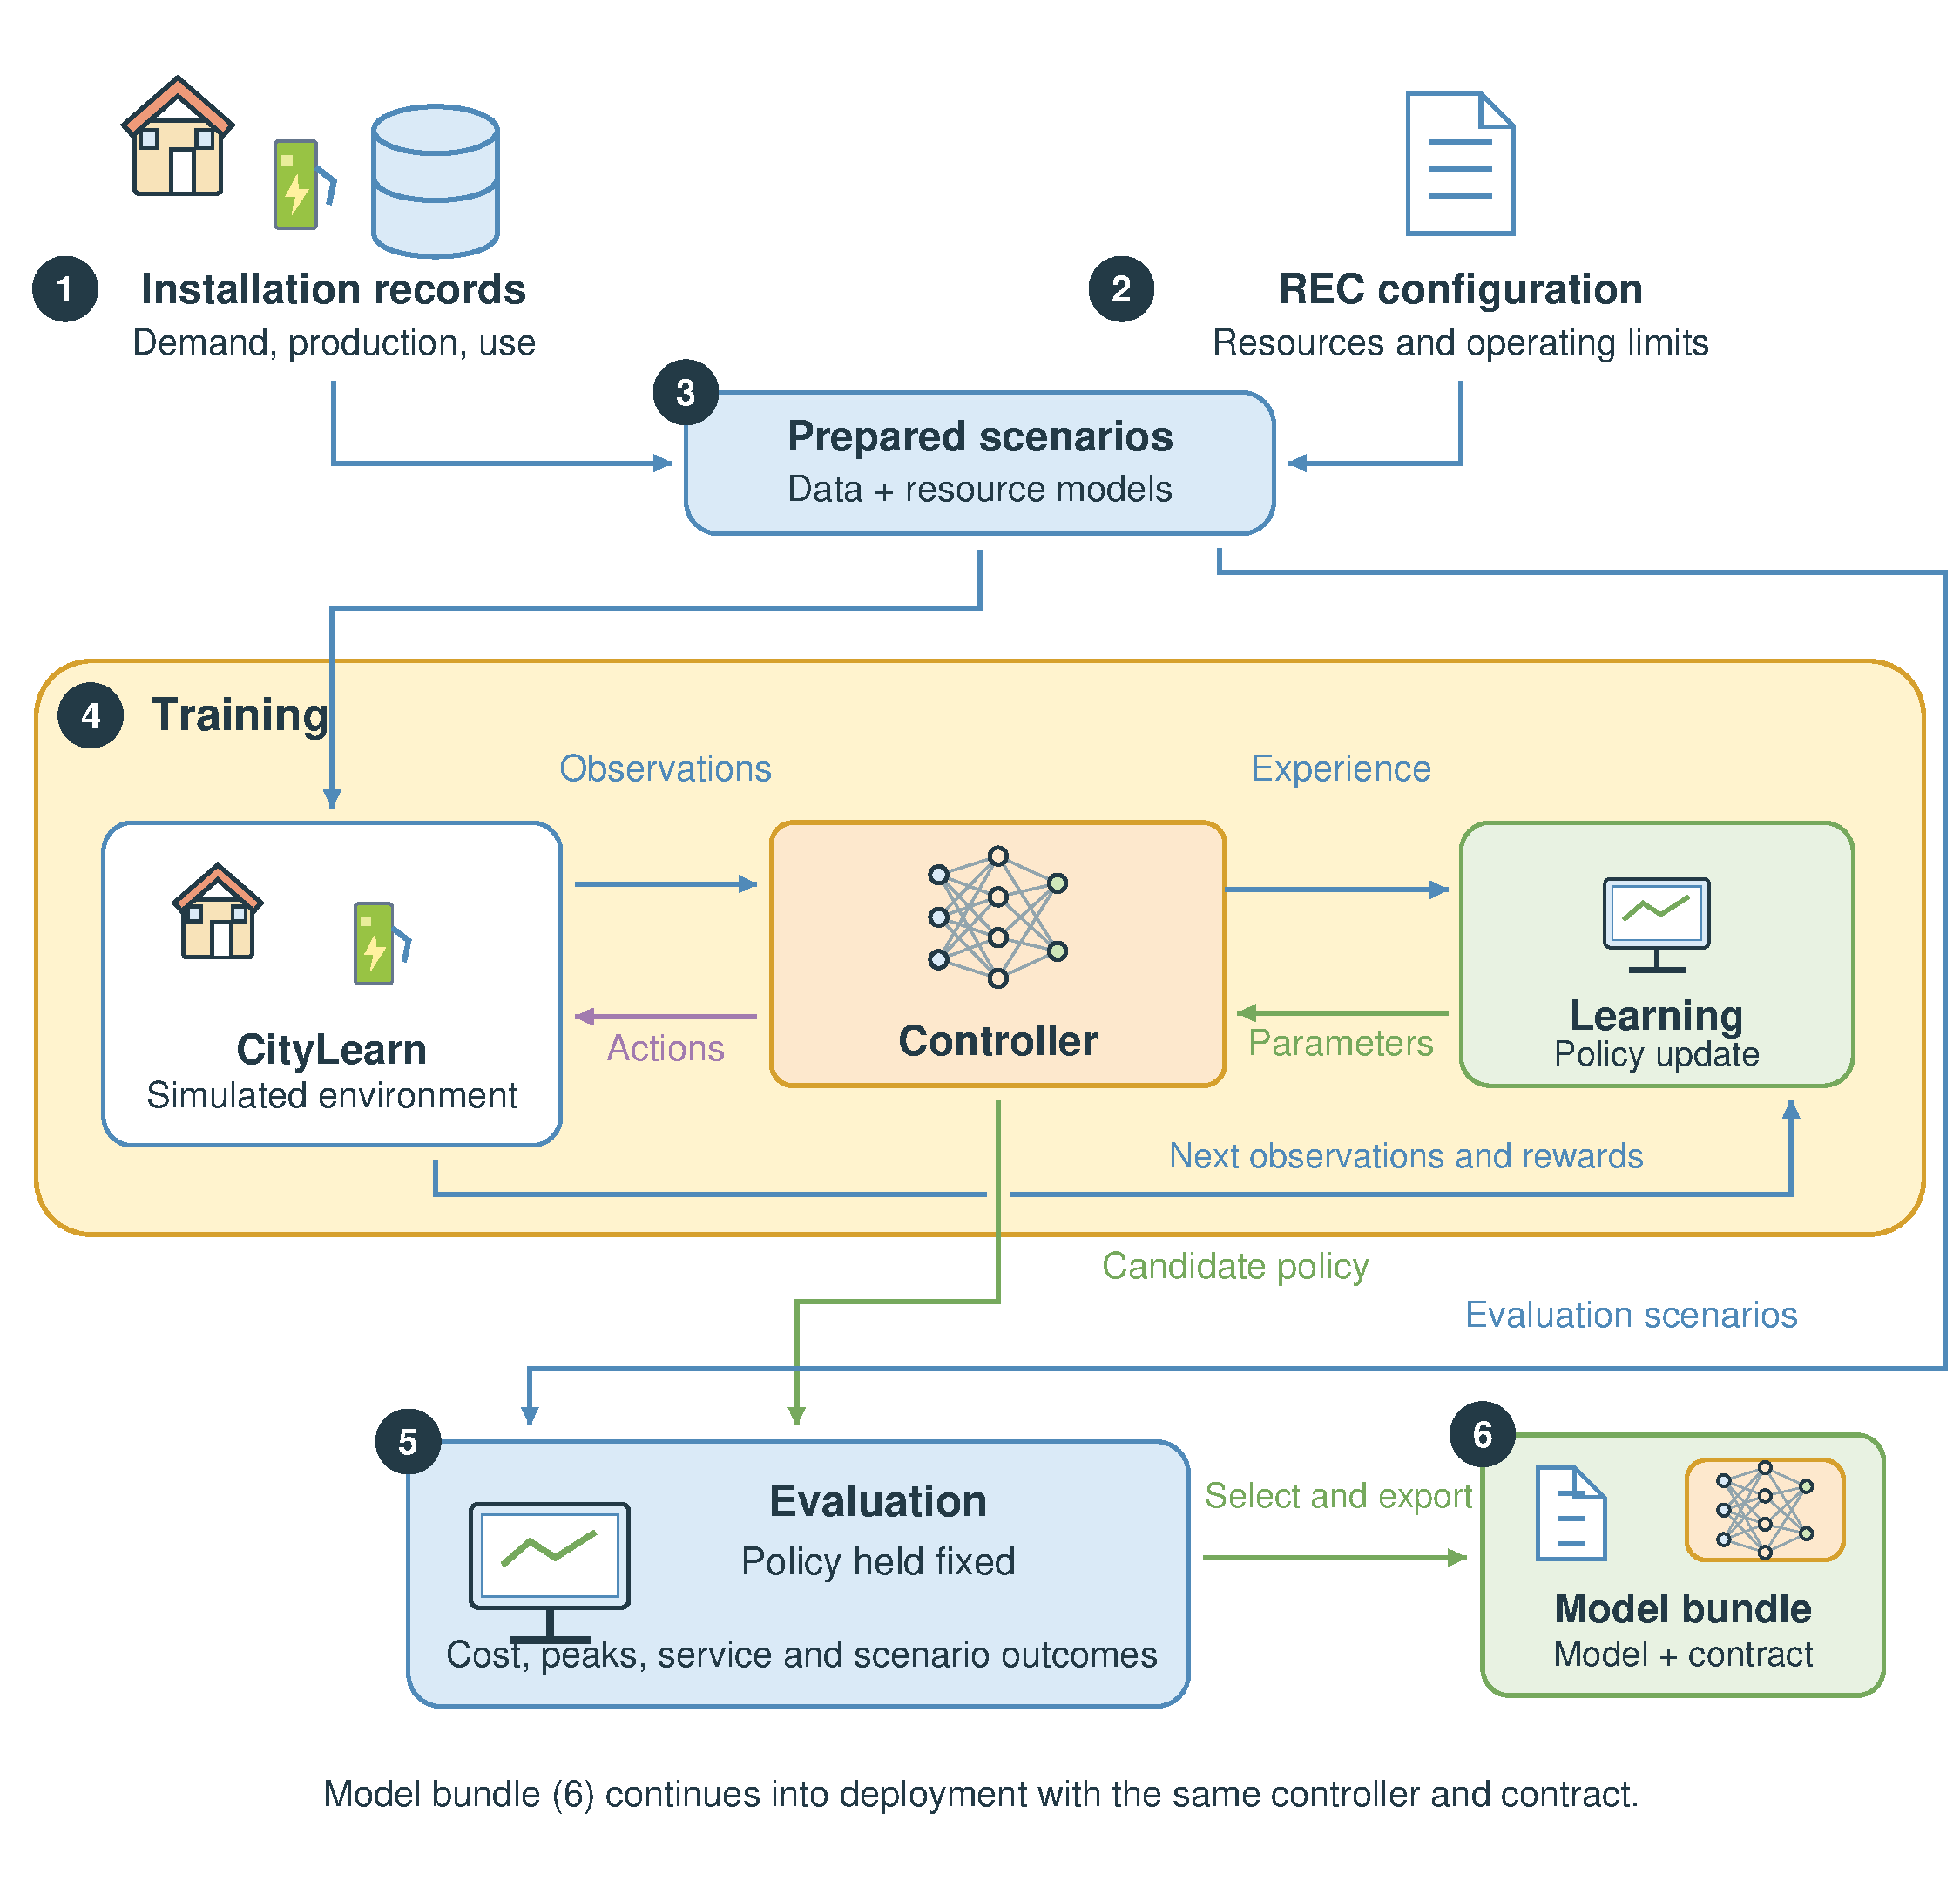
\includegraphics[width=\linewidth]{energaize-controller-development.pdf}
\caption[Controller development through simulation and evaluation.]{Controller development, with the model bundle~(6) continuing into the deployment view.}
\label{fig:energaize-development}
\end{figure}

\subsection{Data Preparation and Simulation Scenarios}
\label{sec:energaize-scenarios}

The household meter, vehicle service, and charger introduced in the runtime view also provide records from which development scenarios can be constructed. These records describe when energy was consumed, when a vehicle was present, and how its charging progressed. Data preparation aligns timestamps, units, and sampling intervals, identifies missing periods, and separates the records used for training from those reserved for evaluation. The \gls{rec} configuration identifies its buildings, equipment, capacities, and operating limits. These describe the setting in which the selected control method is developed.

The building-energy simulator, CityLearn, uses these inputs to represent the environment in which controllers act \parencite{nweye2025citylearnv2}. Vehicle and charger modelling was extended through EVLearn \parencite{fonseca2025evlearn}, and the CityLearn v3 development presented in Chapter~\ref{chap:simulator} supplies the experimental environment used throughout this thesis. Historical demand and production describe the conditions around a decision, while resource models calculate how the controllable equipment responds to it.

The distinction matters for the charging example. Recorded household demand can supply the background load for the evening, but the vehicle's \gls{soc} must evolve according to the actions chosen by the controller being tested. Replaying the recorded charging trajectory would prevent a different decision from changing the outcome. The vehicle model instead updates the stored energy as charging proceeds, subject to its parameters and the charger limits. The next observation reflects that response, allowing the controller to reconsider its decision as the departure approaches.

Supervisor records identify intervals in which a proposal was limited or a fallback supplied the action. These intervals help select conditions to reproduce during development, such as a recurring evening capacity shortage or an interruption in inference. When operational records are used directly as learning experience, the proposed action, validated action, and measured response remain associated. This retains the quantities needed to account for intervention in the learning method, following the distinction in Section~\ref{sec:ch2-constrained-foundations}.

A scenario fixes the conditions of this interaction. It identifies the buildings and resources, the available observations and actions, the external data, and the events encountered during the episode. The arrival at 18:00 and requirement of 80\% by 08:00 can be held constant while several controllers are compared. An earlier departure, a lower connection limit, or an additional vehicle creates a further scenario. These variations let the development process examine particular changes while preserving the settings needed to interpret their consequences.

The scenario also defines the correspondence with runtime. An observation of \gls{soc} belongs to a specified vehicle, and a charging action belongs to a specified charger with a defined unit and range. Forecasts describe information available when the decision is made. Maintaining these associations during simulation prepares the controller for the data and action interfaces through which it will later operate.

\subsection{Controller Training and Evaluation}
\label{sec:energaize-training-evaluation}

With the environment established, \gls{rl} proceeds through repeated interaction. The controller receives the current observations and selects actions for the represented resources. The simulator applies those actions, advances the resource states, and returns the next observations and a reward. The learning procedure uses this experience to adjust the policy. Over successive episodes, the controller encounters the consequences of its choices across complete operating periods.

In the household example, selecting a low charging power may reduce demand during a busy interval, yet leave more energy to be supplied later. The simulated trajectory exposes both effects. The reward expresses the objectives used during learning, while the environment and the controller's feasibility mechanisms represent the applicable constraints. Costs, peaks, and service outcomes can then be examined over the resulting charging session. Their precise formulation depends on the method studied and is developed in the control chapters.

Multi-agent training extends this interaction to the \gls{rec}. Each agent acts for the resources assigned to it, and the environment calculates the combined effect of those actions on buildings and shared quantities. The learning procedure may use information from several agents, even where the resulting controller uses local observations during execution. The development configuration records that distinction: information available to training and information required by the deployed policy have different roles. The runtime interface is determined by the latter.

Evaluation applies a candidate policy with its parameters fixed under scenarios kept separate from training. Common scenarios and information allow comparison with rule-based and other control methods. Energy and service outcomes are read alongside supervisory corrections and fallback use, with the same protection settings retained across a comparison. For the vehicle, a lower cost can then be related to departure readiness, household peak, and the interventions needed to obtain them. Following retraining, comparison with the previous controller also shows how behaviour changes under both the newly identified conditions and the previous evaluation scenarios. Repeated training runs with different random seeds expose variation introduced by learning.

The outcome of this process is a set of results associated with the configuration and model that produced them. Model selection uses those results to identify the controller intended for a particular runtime role. The selected model is exported together with its input and output description, forming the model bundle introduced in Section~\ref{sec:energaize-contract}. Its observation order, processing, and action interpretation must agree with the controller evaluated in simulation.

These stages can require many executions: training several candidates, repeating seeds, and evaluating each controller under several scenarios. Their sequence establishes the work that the infrastructure must support. The next section follows an experiment from its configuration to execution on an available computing resource, then follows the selected model into the inference service.

\section{Experiment Orchestration and Controller Deployment}
\label{sec:orchestration}
\label{sec:energaize-deployment}
\label{sec:lifecycle-governance}

Executing the development process requires a persistent account of each experiment and a way to run it on suitable computing resources. The experiment-management service, the Job Orchestrator, maintains the configuration, queue, and execution record. A Worker Agent connects that record to the machine or remote service that performs the computation. Once a model has been selected, the deployment backend manages its bundle and requests its loading at the chosen inference target. These services carry the controller from an experimental configuration to its place in the runtime architecture.

\subsection{Infrastructure and Experiment Configuration}
\label{sec:energaize-infrastructure}
\label{sec:lifecycle-core}
\label{sec:lifecycle-entities}

\Cref{fig:energaize-orchestration} shows the computing arrangement behind this process. The web interface, backend, and orchestrator run as separate services on the \gls{opeva} server, alongside persistent storage and the workers configured there. The web interface accesses jobs and experiment data through the orchestrator, while the backend provides the deployment interface. A local Worker Agent starts experiment containers through the host's Docker service. Other workers submit work to Deucalion or Union, where the experiment is executed remotely. Personal computers and the Jetson host run their own Worker Agent and experiment containers.

The execution targets provide \glspl{cpu} and, where required, \glspl{gpu}; the worker selects an execution image compatible with the target hardware. Remote submission uses \gls{ssh} or an \gls{api}, according to the target. The Jetson target uses the 64-bit Arm architecture, labelled ARM64 in the figure.

\begin{figure}[H]
\centering
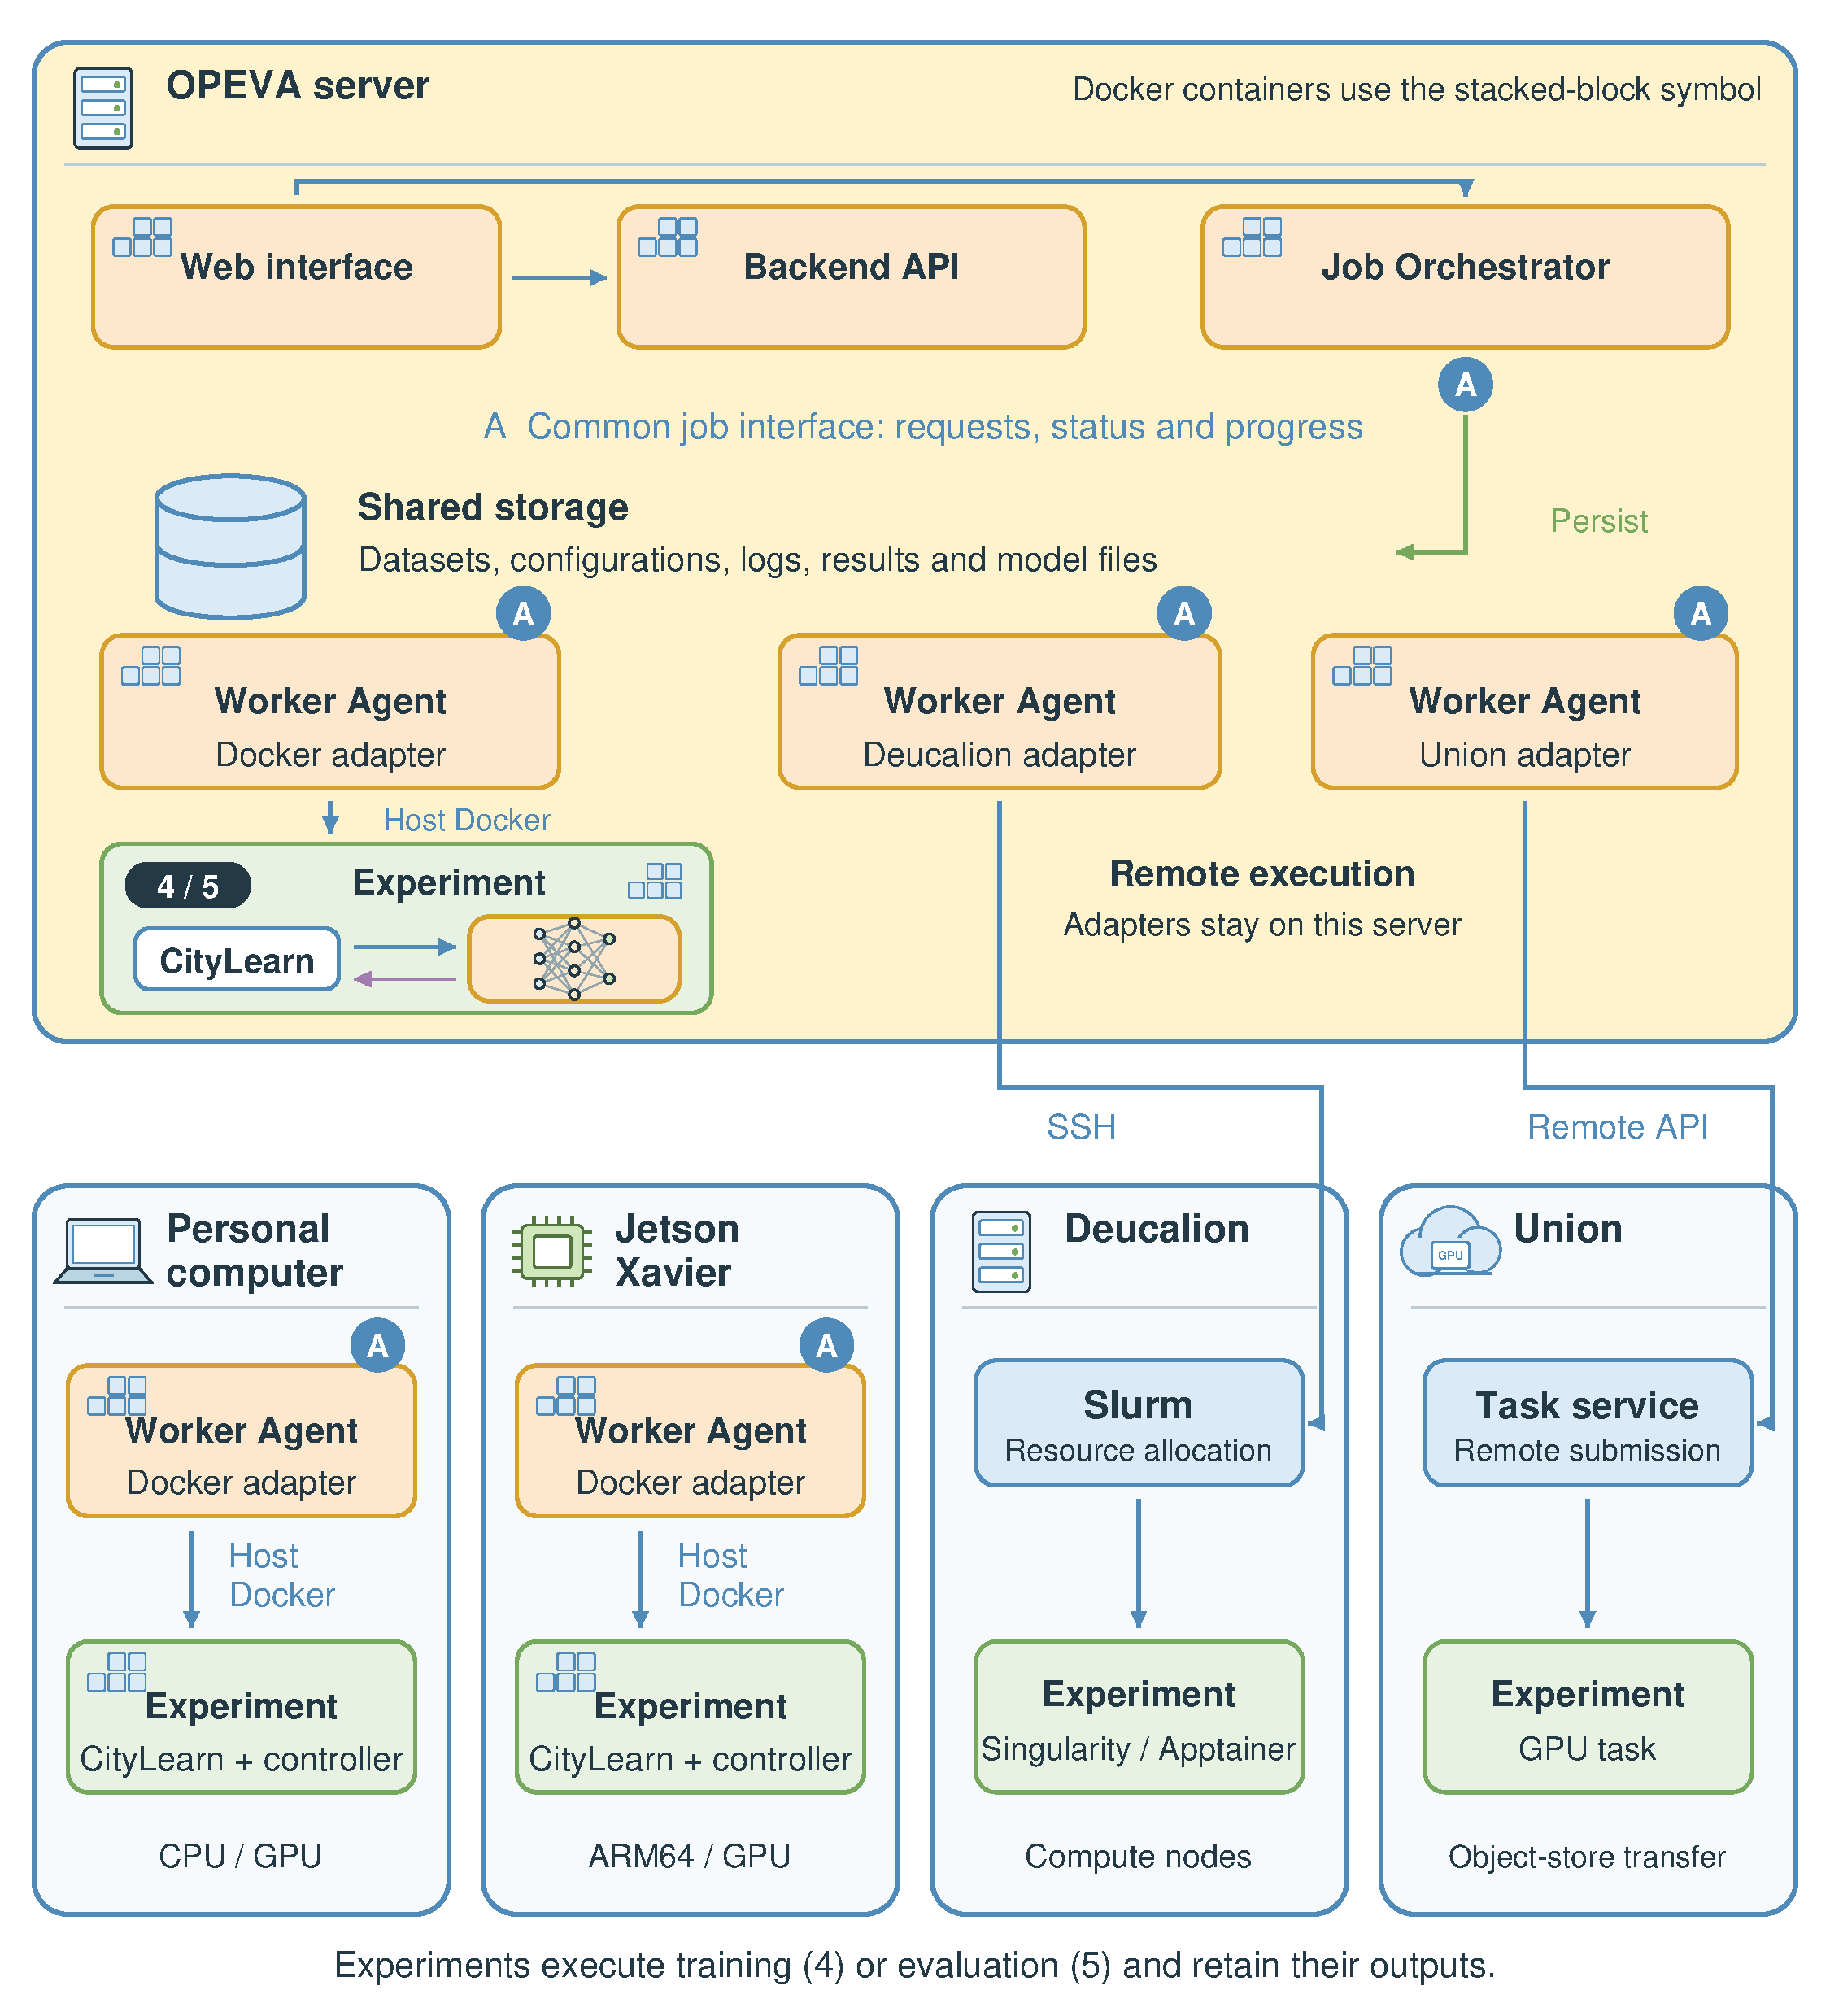
\includegraphics[width=\linewidth]{energaize-orchestration.pdf}
\caption[Computing infrastructure for experiment orchestration.]{Worker Agents manage training~(4) and evaluation~(5) on local or remote resources. The expanded experiment retains the simulator and controller of \cref{fig:energaize-development}.}
\label{fig:energaize-orchestration}
\end{figure}

The worker is a persistent service responsible for obtaining work, launching it, and reporting its progress. The experiment is the process that runs the simulator and control method for one job. With Docker execution, the worker and experiment occupy separate containers on the same host; access to the host's Docker service allows the worker to start and stop the experiment. A remote adapter performs the equivalent management through the target's submission interface. This division allows the experiment software to retain its own dependencies and execution environment while the worker manages its lifecycle.

The experiment configuration combines the \gls{rec} configuration and dataset with the selected controller, observations, actions, reward, random seed, and training or evaluation period. The execution request adds the software image and computing requirements. Resolving these settings before dispatch gives the worker a complete description of the work to perform. The configuration actually executed is retained with the job, so that a later change to a reusable configuration file does not change the account of an earlier experiment.

For the charging example, two runs may use the same controller and household data while assuming different departure times or charging limits. Their interpretation depends on keeping those differences visible. A retraining run likewise has its own configuration and record, even when it continues from an earlier model.

\begin{samepage}
Experiment tracking, model storage, and serving are established concerns in machine-learning operations \parencite{kreuzberger2023mlops,zaharia2018mlflow}. \gls{rl} also requires the environment in which experience is generated \parencite{li2022rlops}. The experiment record therefore retains the simulator and scenario configuration alongside the controller settings.

\end{samepage}

The orchestrator is implemented as a \gls{http} service using FastAPI. Its interface supports experiment submission, job inspection, worker communication, and access to configurations and results. Shared storage retains each job's settings, state, and outputs under a common identity used by the web interface and workers. The experiment can therefore continue independently of the browser session through which it was submitted.

A worker periodically reports its availability, software version, active work, and relevant computing capabilities. When it has capacity, it requests a job that matches its execution profile. The orchestrator supplies the software image, resolved configuration, execution command, and required data locations. The worker then launches the simulator and controller using the execution mechanism of its target. The algorithms receive the configuration prepared for the experiment, while the worker handles the surrounding execution process.

This separation gives each service a clear responsibility. Queueing and job identity remain with the orchestrator; resource-specific execution remains with the worker. The training program can consequently run on a local machine or through a remote scheduler using the same experiment description. Additional workers make it possible to execute independent experiments concurrently, including different random seeds, controller settings, or scenarios.

\subsection{Execution on Heterogeneous Computing Resources}
\label{sec:energaize-compute}

The computing resources used during development have different execution environments. A workstation can start a container directly, a supercomputer admits work through a batch scheduler, and a remote service may require data to be transferred before execution begins. The Worker Agent accommodates these differences through target-specific adapters. Each adapter carries the common job description into the target environment and returns its state and outputs to the orchestrator.

\Cref{tab:lifecycle-targets} summarises the supported execution profiles. The distinction between them concerns how the experiment reaches the processor, obtains its data, and returns its results. The scenario and controller settings remain attached to the same job throughout this process.

\begin{table}[htbp]
\centering
\caption{Computing resources and their execution adapters.}
\label{tab:lifecycle-targets}
\small
\renewcommand{\arraystretch}{1.12}
\begin{tabularx}{\textwidth}{@{}>{\raggedright\arraybackslash}p{0.20\textwidth}>{\raggedright\arraybackslash}p{0.25\textwidth}>{\raggedright\arraybackslash}X@{}}
\toprule
\textbf{Resource} & \textbf{Execution mechanism} & \textbf{Responsibility of the adapter} \\
\midrule
Server & Docker with shared storage & Start the selected image, provide data access, and collect outputs. \\
Personal computer & Docker with optional \gls{gpu} & Connect an intermittently available resource and complete active work before shutdown. \\
Deucalion & Slurm and Singularity/Apptainer & Stage inputs, submit the batch job, follow scheduler state, and retrieve results. \\
Union \gls{inesctec} & Remote tasks with \gls{gpu} resources & Transfer inputs, retain the remote run identity, and recover the returned results. \\
Jetson Xavier & Docker with a compatible NVIDIA image & Match the ARM64 architecture and installed \gls{gpu} software to the execution image. \\
\bottomrule
\end{tabularx}
\end{table}

For server and personal-computer workers, the experiment container reads the configuration and data from mounted storage. For Deucalion, the Worker Agent remains on the submission side. Its adapter creates a remote workspace, stages the required inputs, and submits a Slurm request using a compatible container image. Slurm allocates the computing resources on which the experiment runs through Singularity or Apptainer. Scheduler limits and resource requests become part of that execution setup. Logs are synchronised while the job runs, and the final outputs return to the job's stored record.

The Union Worker Agent similarly remains on the \gls{opeva} side and submits remote tasks. Inputs and results pass through object storage. The worker retains the remote run identity so that monitoring and result retrieval can continue across interruptions. The Jetson profile addresses another form of heterogeneity: its processor architecture and installed \gls{gpu} software require a compatible image. These differences are handled at the worker boundary, where the information needed to execute the experiment is available.

Keeping the adapters behind the common worker interface allows the computing infrastructure to grow without introducing a separate experiment format for each resource. It also preserves information about where and how a result was produced. The software image, execution target, and returned logs remain available when interpreting differences between runs or preparing a further experiment.

\subsection{Job Progress, Results, and Recovery}
\label{sec:energaize-job-recovery}

An experiment passes through several stages before its results are available. After submission and queueing, a worker accepts the job, prepares its execution environment, and starts the training or evaluation process. The job record follows this progression through explicit states. Remote preparation has its own place in that record because transferring a dataset or waiting for a scheduler is different from running the controller inside the simulator.

Progress updates and logs make this distinction useful to the operator. The EnergAIze web interface displays the queue, worker availability, execution state, training progress, and completed outputs. It also provides access to configurations and \gls{kpi} comparisons, with links to MLflow records where tracking is enabled. These views connect the visible result to the experiment that produced it. For a charging study, the operator can inspect cost and peak demand alongside the departure charge, then return to the corresponding scenario and controller settings.

Persistent state also supports recovery when communication or execution is interrupted. Each dispatched attempt can carry an identifying token that the worker returns with its updates. If a job is reassigned, updates from the superseded attempt are rejected. This prevents a delayed worker from replacing the state or results of a newer execution. A stop request follows the same division of responsibility: the orchestrator records the request, and the worker stops the container or remote job that it manages.

Remote result retrieval requires particular care. A training process may finish successfully while the connection needed to download its outputs is unavailable. In the Union adapter, a recovering state records this interval between completed computation and locally available results. The remote run identity and recovery progress are persisted, allowing the transfer to resume after the worker restarts. The completed training outputs can then be recovered without repeating the experiment. Deucalion similarly retains the connection between the local job and the remote scheduler record while its adapter monitors execution and retrieves the outputs.

Once execution and result retrieval are complete, model selection can use the recovered evidence. The selected controller then needs a description that allows the inference service to reconstruct the input processing and action interpretation used during evaluation. This is the role of the model contract.

\subsection{The Model Contract}
\label{sec:energaize-contract}

The selected model is exported with a model contract that preserves its input and output settings: observation names, ordering and encoding, returned actions, and agent--model associations. This manifest and the model files form the \emph{model bundle}~(6) shown in the development and deployment views. The full experiment configuration remains in the job record.

\Cref{tab:energaize-model-contract} groups the information passed through this interface. The installation configuration supplies the connection to physical equipment and its provider interfaces. The model contract supplies the interpretation required by the selected controller. Their correspondence is what allows an observation assembled by Percepta to reach the intended input and a returned action to be directed to the correct resource.

\begin{table}[htbp]
\centering
\caption{Information carried by the model contract.}
\label{tab:energaize-model-contract}
\small
\renewcommand{\arraystretch}{1.12}
\begin{tabularx}{\textwidth}{@{}>{\raggedright\arraybackslash}p{0.24\textwidth}>{\raggedright\arraybackslash}X>{\raggedright\arraybackslash}X@{}}
\toprule
\textbf{Part of the contract} & \textbf{Stored information} & \textbf{Use in runtime} \\
\midrule
Observations & Names, ordering, and input encoders & Reconstruct the input representation used during development. \\
Actions & Names, bounds, and output settings & Return identifiable actions in the form expected by the integration path. \\
Agents and models & Agent indices, model format, and file locations & Select the model associated with the requested agent. \\
Origin and configuration & Run identity and accompanying environment metadata & Associate the loaded controller with its development record. \\
\bottomrule
\end{tabularx}
\end{table}

For the household vehicle, the contract determines where \gls{soc} enters the model and how the returned charging decision is named. If the model was trained with encoded calendar variables or a particular observation order, the inference service reconstructs that processing when it loads the bundle. A controller serving several agents also needs the association between each agent and its model. This association can point to separate model files or to a shared model used by several agents.

The general export path produces neural models in the \gls{onnx} format and rule-based policies in \gls{json}. Before the bundle is finalised, validation checks the manifest structure, declared formats, referenced files, agent indices, and observation and action dimensions. The resulting package can be passed from the experiment implementation to the inference service without manually rebuilding its feature ordering or action mapping. The control methods developed in Chapters~\ref{chap:control-benchmark} and~\ref{chap:ti-marl} supply any additional requirements for their runtime components.

\subsection{Controller Deployment and Updates}
\label{sec:policy-registry}
\label{sec:edge-deploy}
\label{sec:lifecycle-monitoring}

The deployment backend maintains a catalogue of model bundles in shared storage. Each stored bundle retains its manifest and model files under a content-derived identity. The web interface allows the operator to inspect the available bundles and select a version for an inference target. A target is the service endpoint at which the selected controller will be loaded; the installation configuration determines which observations and equipment are associated with that service.

\Cref{fig:energaize-deployment} continues from the same model bundle~(6), through catalogue storage~(7), operator selection~(8), and backend loading~(9). The controller runs inside the inference service, using the runtime connections shown in \cref{fig:energaize-overview}.

\begin{figure}[htbp]
\centering
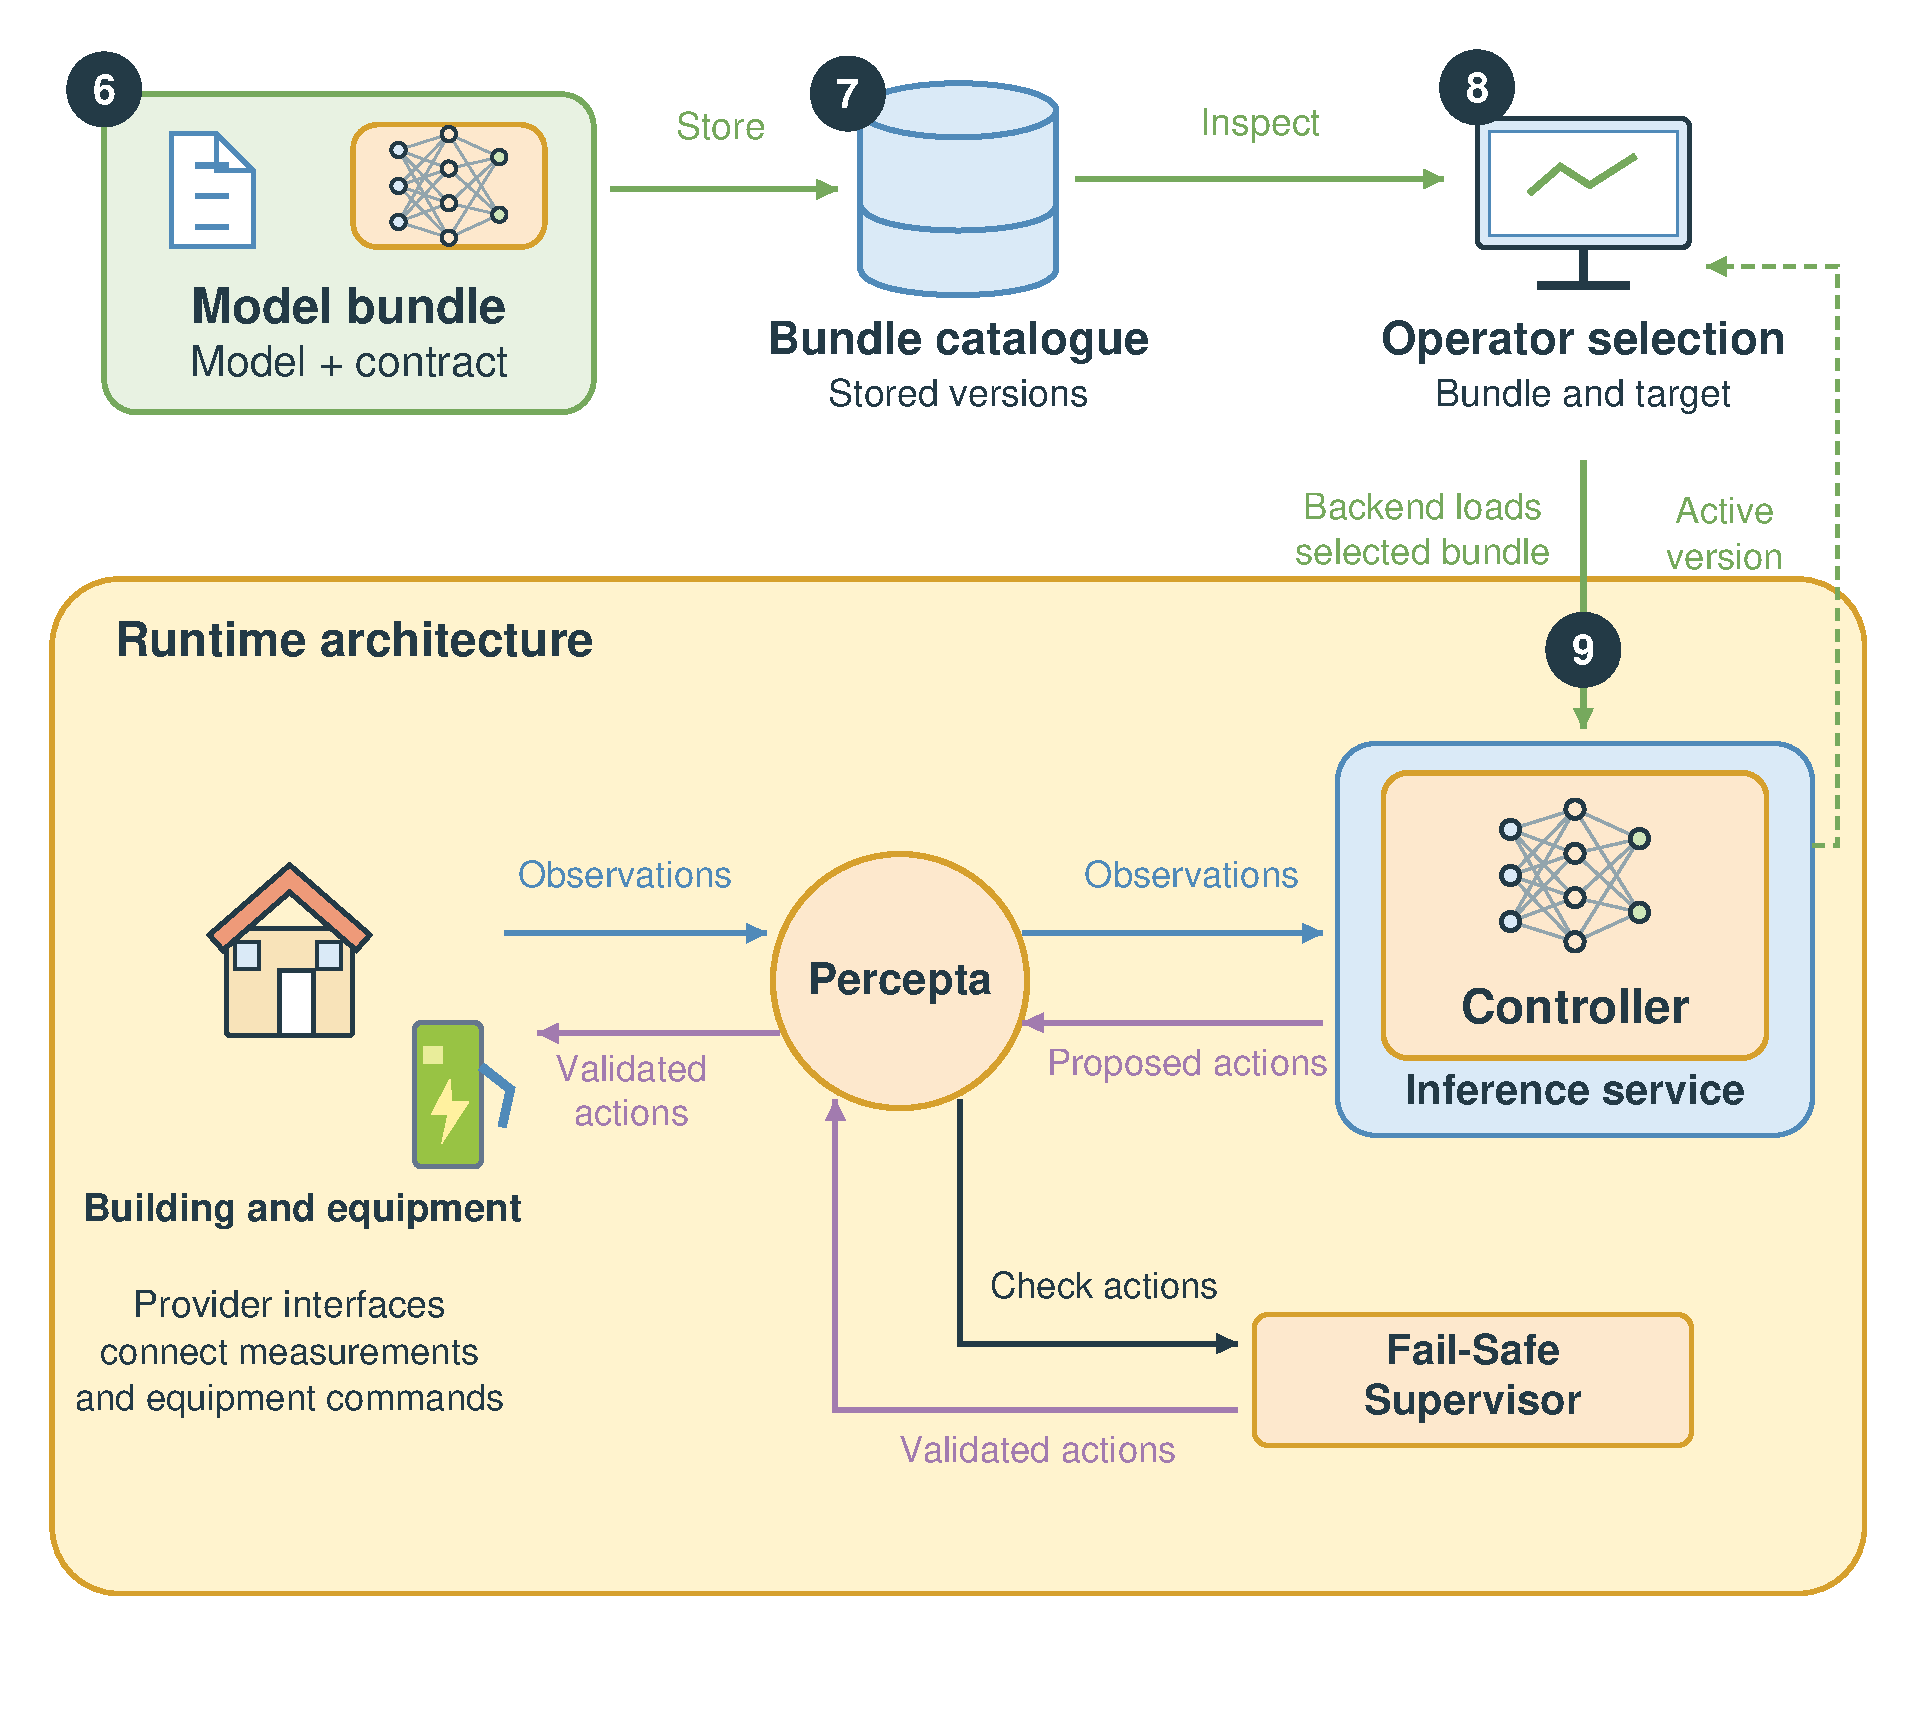
\includegraphics[width=\linewidth]{energaize-model-deployment.pdf}
\caption[Model deployment and the runtime control loop.]{Model deployment~(6--9) and the controller within the runtime control loop.}
\label{fig:energaize-deployment}
\end{figure}

For the selected target, the backend resolves the stored bundle location and sends a loading request to the inference service. The service reads the manifest, locates the model files, prepares the input encoders, and creates the appropriate \gls{onnx} or rule-based executor. It then reports the loaded configuration and agent indices, making the active controller visible to the backend and web interface.

During operation, health information exposes the service's readiness, while request identifiers associate inference calls with their responses. The records described in Section~\ref{sec:energaize-records} connect the loaded controller to supervisory interventions, provider responses, and subsequent measurements. An operator can consequently follow a charging request from the selected model to the power delivered at the installation.

Updates use the same loading path. The operator selects a new bundle for the target and inspects the reported active version after loading. Earlier bundles can remain in the catalogue and be selected again when a previous controller is required. The backend protects a bundle reported as active by a reachable target from deletion, preserving the files associated with that deployment. Each target exposes its own loaded state, allowing the operator to follow changes across installations.

The operational records retained during deployment supply the datasets and cases used for subsequent development. An operator can revisit intervals with repeated corrections or fallback use, together with changes in connection times, equipment, or operating limits. These findings guide scenario revisions, configuration updates, or controller retraining through the same orchestration service. The resulting candidate is evaluated through the process in Section~\ref{sec:energaize-training-evaluation}, after which the operator can select its model bundle for deployment. Its development record retains the connection to the operating conditions that motivated the update.

\section{Chapter Summary}
\label{sec:energAIze-forward-map}
\label{sec:energaize-chapter-map}

EnergAIze connects \gls{rec} energy control to the services needed to develop and operate its controllers. Runtime integrates observations, controller execution, independent supervision, and equipment interfaces. Development uses data and simulation to train and evaluate candidates, with the Job Orchestrator and Worker Agent managing experiment execution. The deployment backend loads the selected model bundle into the inference service. Operational records return measured outcomes and supervisory interventions to development, supporting later retraining and evaluation.

These connections give architectural form to the four dimensions established in Chapters~\ref{chap:introduction} and~\ref{chap:related-work}. For \emph{scalability}, \gls{rec} configurations and experiment records allow control outcomes to be related to the system's size, composition, and computing requirements. For \emph{deployability}, the model contract, development services, and equipment interfaces organise preparation, training and adaptation, integration, and maintenance so that evaluated behaviour can be reproduced and sustained. \emph{Safety} is addressed through constraint enforcement and separate records of proposals, supervisory intervention, and equipment response. \emph{Robustness} draws on service monitoring, fallback control, and recovery, with retained service examined under the conditions recorded during operation.

Chapter~\ref{chap:simulator} develops the simulation environment used to represent buildings and resources and compare their controllers. Chapters~\ref{chap:control-benchmark} and~\ref{chap:ti-marl} develop the control methods, while Chapter~\ref{chap:real-world} examines their integration and use in operating installations.

\setlength{\parskip}{\architectureoriginalparskip}
\clearpage
\setlength{\textfloatsep}{\architectureoriginaltextfloatsep}
\setlength{\intextsep}{\architectureoriginalintextsep}
\setlength{\abovecaptionskip}{\architectureoriginalcaptionskip}
\flushbottom
\clubpenalty=\architectureoriginalclubpenalty
\widowpenalty=\architectureoriginalwidowpenalty

\chapter{Simulation and Evaluation of Renewable Energy Communities: CityLearn v3}
\label{chap:simulator}
\markboth{Simulation and Evaluation Environment}{Simulation and Evaluation Environment}

% Keep displayed equations with the opening of their symbol definitions.
\begingroup
\raggedbottom
\postdisplaypenalty=10000

The architecture in Chapter~\ref{chap:energAIze} places simulation between the preparation of \gls{rec} data and the evaluation of a controller. This chapter develops that experimental environment: the extensions to CityLearn, the \gls{rec} datasets, and the methods used to check the simulator and compare control decisions. Together, these provide the experimental foundation for the learning methods in Chapters~\ref{chap:control-benchmark} and~\ref{chap:ti-marl}.

\section{Development of the Simulation Environment}
\label{sec:sim-research-contribution}
\label{sec:sim-motivation}
\label{sec:sim-inherited-gap}
\label{sec:sim-lineage}
\label{sec:sim-sota}
\label{sec:sim-iterative-instrument}

Preparing a controller for operation requires an environment in which its decisions have consequences over time. Charging a vehicle now changes the energy still needed before departure; using a battery changes the flexibility available later; and sharing \gls{pv} production changes the exchanges of several members. In the development process described in Chapter~\ref{chap:energAIze}, simulation provides this continuity. It allows a controller to learn from repeated interactions and to be evaluated under specified \gls{rec} conditions before it is selected for deployment.

An established building-energy environment, CityLearn, provided the starting point. Its building and storage models, common controller interface, and energy indicators already supported multi-building control studies \parencite{vazquezcanteli2019citylearn,nweye2025citylearnv2}. Shared tasks and datasets, including the CityLearn Challenge, had also established a common setting for comparing research methods \parencite{nagy2021citylearnchallenge}. Developing within this environment connected the work to an existing research community and allowed the new capabilities to be used alongside established models and controllers.

The contribution developed in this thesis extends that foundation with \gls{rec} resources, operating events, controller interfaces, and evaluation methods. It began with the integration of \glspl{ev} through EVLearn, which introduced chargers, connection schedules, departure requirements, and bidirectional charging \parencite{fonseca2025evlearn}. Work on \gls{rec} control, informed by \gls{opeva} and DemFlex, then required a broader representation of how installations operate. Members could join or leave, equipment could change, flexible appliances had complete programmes to deliver, and local sharing affected individual costs. Measurements and commands could also fail. These conditions shaped the subsequent development of CityLearn v3 and the experiments it needed to support \parencite{fonseca2026citylearnv3}.

Accommodating them involved changes across the simulation process. Installing a charger, for example, introduces a physical resource, an action that a controller can request, and future charging services whose outcomes must be recorded. Its identity and activation time therefore have to agree across scenario loading, state progression, controller inputs, and evaluation. Similar connections arise when a member leaves or an action cannot be applied. The work extended these parts together so that an experiment could follow a change from its declaration to its effect on energy use and participant service.

These extensions give the \glspl{rq} in Chapter~\ref{chap:introduction} concrete experimental settings. A changing resource collection exposes the adaptation and computational demands of scalability; electrical limits and participant services establish the conditions for examining safety; and repeatable failures make robustness comparisons possible. The controller interface also carries the resource and action descriptions needed by the deployment process in Chapter~\ref{chap:energAIze}. The following control chapters use this foundation to investigate how the methods respond.

\label{sec:sim-public-release}
The resulting software was first distributed by the \gls{softcps} Research Group as the \gls{softcps} \gls{rec} Simulator \parencite{softcps2026simulatorrepo,softcps2026pypi}. In September 2026, this development line was incorporated into the official CityLearn version~3, distributed as \texttt{citylearn} \parencite{citylearn2026v3release}. Its Gymnasium interface, examples, documentation, and tests make the extensions available through the established project \parencite{citylearn2026official}. The contribution thus provides both the experimental environment used in this thesis and reusable modelling and evaluation capabilities for other \gls{rec}-control studies.

\section{Community Modelling and Simulator Architecture}
\label{sec:sim-architecture}
\label{sec:sim-deployment-pipeline}

The simulator represents buildings and their resources within one or more \glspl{rec}. In the scenarios used here, each member is represented by one building site, with a local agent managing that site's assets. This modelling convention instantiates the distinctions in Section~\ref{sec:ch2-rec-members}; it does not equate members, sites, and agents in the general definition. A scenario supplies their data, connections, services, and operating events; a controller receives observations and proposes actions as the simulation advances. Figure~\ref{fig:sim-architecture} locates these interactions. Each \gls{rec} retains its own members, local sharing, and outcomes, while a common environment can advance several \glspl{rec} together.

The changes shown in the figure are part of the model: a member leaves, a charger is installed, and data or equipment become unavailable. Each changes a different aspect of the decision faced by the controller. The following subsections explain how these conditions are represented and how the implementation makes their consequences available for subsequent experiments.

\begin{figure}[htbp]
\centering
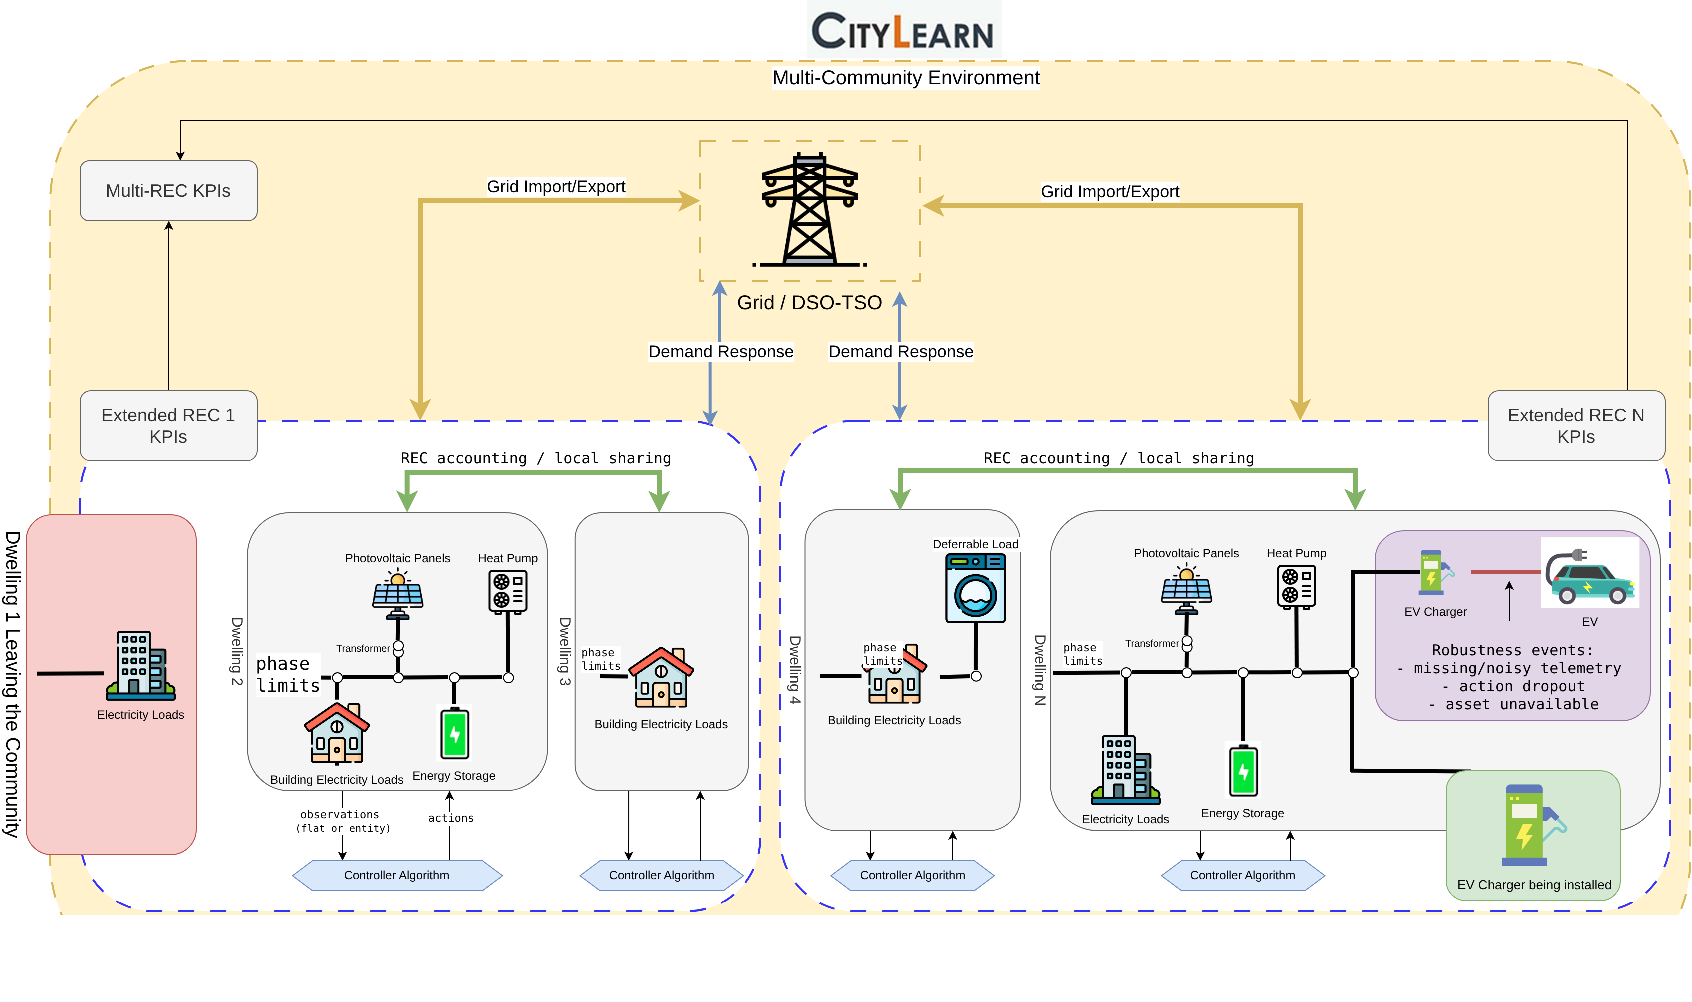
\includegraphics[width=1.0\textwidth]{simulator-environment-architecture.pdf}
\caption{Representation of one or more \glspl{rec} in CityLearn v3. Reproduced from \textcite{fonseca2026citylearnv3}.}
\label{fig:sim-architecture}
\end{figure}

\subsection{Scenarios, Time, and the Simulation Step}
\label{sec:sim-contracts}

A scenario combines time series with the information needed to interpret them. It identifies the buildings and equipment, their capacities and connections, the services to deliver, the observations exposed to a controller, and the events active during the episode. This configuration distinguishes two experiments that use identical household demand but differ in charging availability, an electrical limit, or a missing measurement.

\begin{samepage}
At timestep $t$, the simulator first resolves scheduled changes and constructs the available observations. The controller then proposes an action, which passes through the applicable feasibility and availability rules before the resources advance:
\begin{equation}
\begin{aligned}
\tilde{o}_t&=\mathcal{O}(x_t,w_t,e_t), & a_t^{\mathrm{req}}&=\pi(\tilde{o}_t),\\
a_t^{\mathrm{app}}&=\Gamma(a_t^{\mathrm{req}},x_t,e_t), & (x_{t+1},y_t)&=F(x_t,a_t^{\mathrm{app}},w_t,e_t).
\end{aligned}
\label{eq:sim-step-contract}
\end{equation}
Here, $x_t$ is the represented physical and service state, $w_t$ contains external inputs such as demand and weather, and $e_t$ contains active events. The observation function $\mathcal{O}$ produces the controller-visible information $\tilde{o}_t$, and policy $\pi$ returns requested action $a_t^{\mathrm{req}}$. Operator $\Gamma$ accounts for the configured limits, availability, and command handling to obtain applied action $a_t^{\mathrm{app}}$. The transition function $F$ produces the next state $x_{t+1}$ and the physical, service, and accounting outcomes $y_t$.\par
\end{samepage}

For the charging example, the \gls{soc} after an interval depends on the power actually applied. Retaining the original request makes it possible to distinguish a controller that respects the connection limit from one whose proposals repeatedly require correction, even when both produce the same physical trajectory. This separation gives the safety experiments access to the decision and its execution. It corresponds to the controller, supervisor, and equipment roles described in Section~\ref{sec:energaize-runtime}.

Time and units are part of this interpretation. Power and instantaneous limits use kW, interval energy uses kWh, prices use currency/kWh, and carbon intensity uses kgCO$_2$/kWh. Average power converts to interval energy through
\begin{samepage}
\begin{equation}
E_t=P_t\frac{\Delta t}{3600},
\label{eq:sim-power-energy}
\end{equation}
where $E_t$ is energy in kWh during interval $t$, $P_t$ is its average power in kW, and $\Delta t$ is the interval duration in seconds. The factor 3600 converts seconds to hours. A \SI{7.2}{\kilo\watt} charger consequently supplies \SI{1.8}{\kilo\watt\hour} in 15 minutes or \SI{0.03}{\kilo\watt\hour} in 15 seconds.\par
\end{samepage}

The same care applies to \gls{pv} inputs. A normalised production profile is scaled by installed capacity, whereas an absolute production series already describes the site's output. The loader checks the declared clock, timestamp spacing, and episode bounds. Columnar storage and windowed loading make short timesteps practical for repeated learning experiments without requiring each run to process an entire high-frequency dataset.

Figure~\ref{fig:sim-high-frequency} illustrates why temporal resolution matters to safety-sensitive studies. It represents the same synthetic annual trace at one-hour, 15-minute, and 15-second resolution. The annual energy is preserved, while the visible peak rises from 96.8 to 188.2 and 281.5~kW as shorter intervals retain events hidden by averaging. A simulator intended to study electrical headroom therefore needs an explicit clock and consistent energy accounting; the experiment can then choose the resolution appropriate to its control question \parencite{fonseca2026citylearnv3}.

\begin{figure}[htbp]
\centering
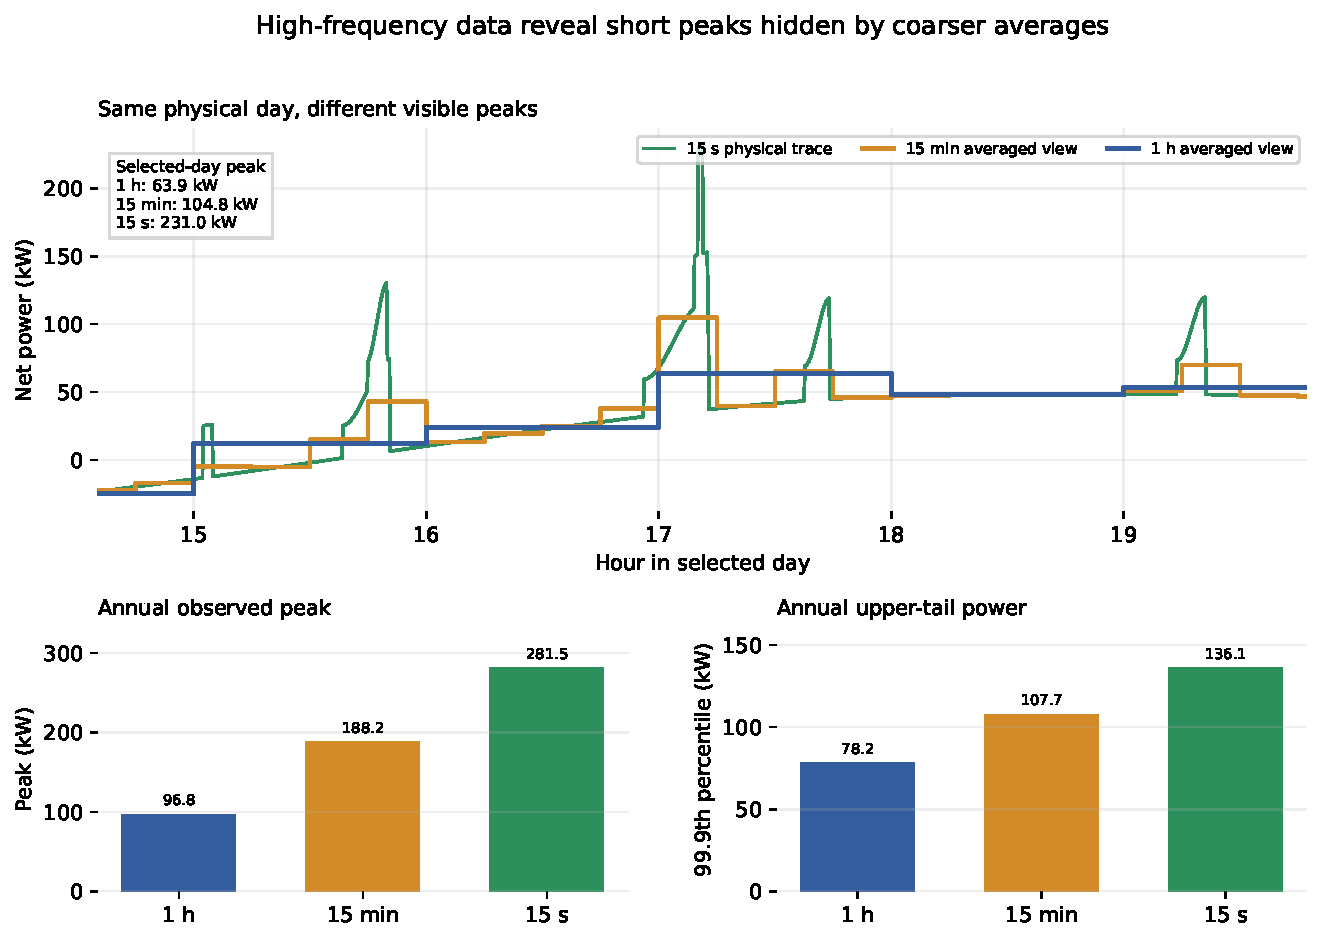
\includegraphics[width=0.96\textwidth]{simulator-high-frequency.pdf}
\caption{Peak visibility at three temporal resolutions of the same synthetic annual trace.}
\label{fig:sim-high-frequency}
\end{figure}

\subsection{Resources, Electrical Limits, and Participant Services}

Buildings retain background demand, \gls{pv} generation, grid exchange, and their available flexibility resources. Inherited thermal and storage components preserve compatibility with established CityLearn studies. The extensions developed here connect stationary storage, \gls{ev} charging, and complete appliance cycles to the services and electrical conditions of each installation.

\paragraph{Stationary storage and electrical headroom.}
A stationary battery has an energy capacity, charging and discharging power, efficiency, and state-of-charge limits. Its admissible exchange changes with stored energy and with the headroom available at the building. Charging a battery and a vehicle at the same time may therefore require less power than either device could accept alone.

\begin{samepage}
The electrical model represents total import/export limits and, where configured, separate limits for each phase. With import taken as positive, the limits are
\begin{equation}
-X_b^{\max}\leq P_{b,t}\leq I_b^{\max},\qquad
-X_{b,\phi}^{\max}\leq P_{b,\phi,t}\leq I_{b,\phi}^{\max}\quad\forall\phi\in\Phi_b.
\label{eq:sim-electrical-limits}
\end{equation}
Here, $b$ is a building, $t$ the timestep, and $\Phi_b$ its electrical phases. Total and phase power are $P_{b,t}$ and $P_{b,\phi,t}$; $I^{\max}$ and $X^{\max}$ denote the positive import and export limits. All powers are in kW.\par
\end{samepage}

If the house already imports \SI{4}{\kilo\watt} on a phase limited to \SI{7}{\kilo\watt}, a \SI{7.2}{\kilo\watt} charging request has only \SI{3}{\kilo\watt} of headroom. Representing the connection as well as the device rating exposes this competition between simultaneous uses. Requested pressure measures the excess before constraint handling, while residual violation measures exceedance in the applied trajectory, including cases where background demand alone exceeds a limit. Section~\ref{sec:sim-service-evaluation} defines how these quantities enter the safety comparison.

\paragraph{Vehicles and charging sessions.}
A charging session specifies the connected vehicle, arrival \gls{soc}, departure time, requested departure state, and applicable power bounds. These quantities determine the remaining energy requirement and the time in which it can be met. As 08:00 approaches, the same postponement that was harmless at 18:00 may make the target unreachable. The simulator follows battery response through the session and evaluates service at departure.

The model gives the vehicle, physical charging port, and session separate identities. When the example vehicle leaves at 08:00, another vehicle may use the same port later that day: the service requirement changes while the installed equipment remains the same. Adding a second port changes the resources the controller can address. This separation allows experiments to vary service demand and resource composition independently, and to associate each departure outcome with the correct request.

The vehicle catalogue can link visits across sites. In the dataset runtime used here, each session supplies its arrival \gls{soc}; battery evolution then follows the applied charging power until departure. A window beginning during an occupied session uses the corresponding boundary state. The departure record compares achieved \gls{soc} with the requirement and gives the remaining energy deficit. Lower electricity consumption can therefore be read alongside the service actually delivered.

\paragraph{Deferrable appliances.}
A deferrable appliance offers a different decision: when to begin a complete programme. A cycle catalogue supplies the interval-energy profile and duration, while a request supplies an admissible start window, completion deadline, and service priority. Choosing a start commits the simulation to that programme. This preserves its energy and duration when a controller shifts it towards a favourable price or a period of solar production.
\begin{samepage}
\begin{equation}
t_c^{\mathrm{earliest}}\leq s_c\leq t_c^{\mathrm{latest}},\qquad s_c+d_c-1\leq t_c^{\mathrm{deadline}}.
\label{eq:sim-deferrable-feasibility}
\end{equation}
Here, $c$ identifies a requested cycle, $s_c$ is its selected start timestep, and $d_c$ is its duration in timesteps. The quantities $t_c^{\mathrm{earliest}}$, $t_c^{\mathrm{latest}}$, and $t_c^{\mathrm{deadline}}$ are the earliest start, latest start, and final admissible completion timestep. For a discrete profile $q_{c,\tau}$, the index $\tau$ denotes the interval within the cycle and $q_{c,\tau}$ gives its energy demand.\par
\end{samepage}

\begin{figure}[htbp]
\centering
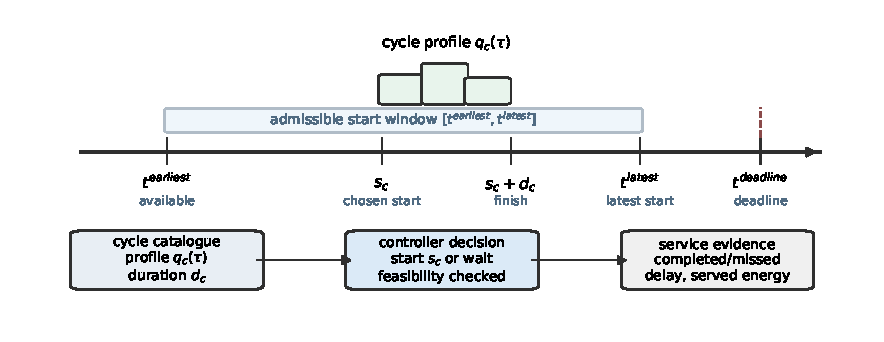
\includegraphics[width=0.96\textwidth]{simulator-deferrable-cycle.pdf}
\caption{A complete appliance programme scheduled within its admissible start window.}
\label{fig:sim-deferrable-cycle}
\end{figure}

Figure~\ref{fig:sim-deferrable-cycle} relates the scheduling choice to the complete service. Once a cycle starts, its progress is followed alongside electrical limits. Completed and missed cycles, delay, delivered energy, and unserved energy make the consequence visible. This permits the evaluation to distinguish demand shifted successfully from demand simply left unserved.

\subsection{Local Sharing and Demand-Response Services}

An aggregate \gls{rec} balance can hide simultaneous import and export by different participants. The simulator calculates local sharing in each interval, preserving the coincidence of demand and surplus, and settles that exchange at member level. A neighbour can then benefit from solar production when it is available, while storage and scheduling determine how much demand can be moved into that interval. Member demand, local exchange, and residual grid exchange remain separate quantities.

\begin{samepage}
For the active member set $\mathcal{C}_t$, local sharing is bounded by simultaneous demand and surplus:
\begin{equation}
\begin{aligned}
D_{\mathcal{C},t}&=\sum_{b\in\mathcal{C}_t}\max(E^{\mathrm{net}}_{b,t},0),\\
S_{\mathcal{C},t}&=\sum_{b\in\mathcal{C}_t}\max(-E^{\mathrm{net}}_{b,t},0),\\
L_{\mathcal{C},t}&=\min(D_{\mathcal{C},t},S_{\mathcal{C},t}).
\end{aligned}
\label{eq:sim-local-sharing}
\end{equation}
Here, $E^{\mathrm{net}}_{b,t}$ is member $b$'s net interval energy at time $t$, positive for demand and negative for surplus. For active members $\mathcal{C}_t$, $D_{\mathcal{C},t}$, $S_{\mathcal{C},t}$, and $L_{\mathcal{C},t}$ denote total demand, surplus, and locally shared energy, all in kWh.\par
\end{samepage}

Participant weights allocate the available exchange within demand and supply, and remaining energy passes through the grid boundary. The scenario defines the price of local exchange and the remuneration of residual export.

The settlement example in Figure~\ref{fig:sim-rec-settlement} applies two accounting rules to the same historical 17-member trajectory. Under the configured sharing rule, 17.0~MWh is exchanged locally and total cost changes from 24.8 to 22.0~kEUR. Individual savings range from 68.8 to 525.7~EUR. The implementation retains this distribution because the \gls{rec} total alone cannot show which participants benefit from the available flexibility \parencite{fonseca2026citylearnv3}.

\begin{figure}[htbp]
\centering
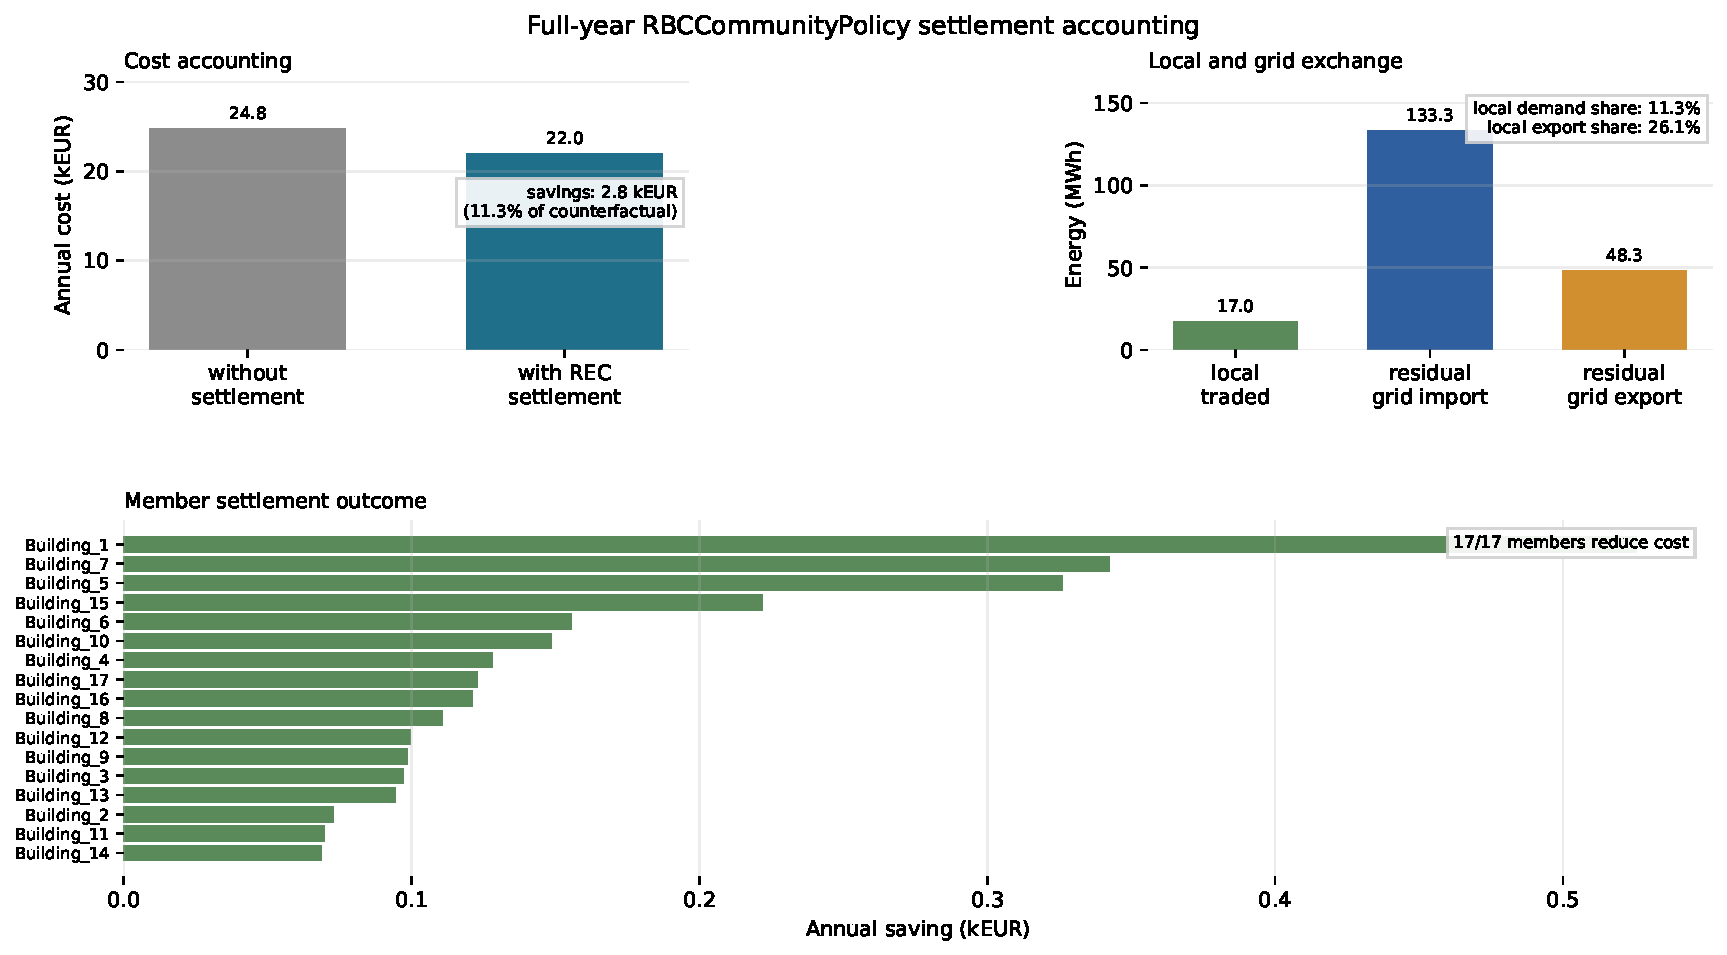
\includegraphics[width=0.96\textwidth]{simulator-rec-settlement.pdf}
\caption{\gls{rec} and participant outcomes under two accounting rules for the same historical trajectory.}
\label{fig:sim-rec-settlement}
\end{figure}

\gls{dr} introduces a service requested from outside the \gls{rec}. Each request declares its issuer, direction, interval, target power, tolerance, remuneration, penalty, and reference method. Keeping the request explicit distinguishes service delivery from an ordinary response to price. For a reduction request, charging the example vehicle later can release power now, provided its departure requirement remains achievable.
\begin{samepage}
\begin{equation}
d_{r,t}=\begin{cases}P_t-B_{r,t},&\text{up request},\\B_{r,t}-P_t,&\text{down request}.
\end{cases}
\label{eq:sim-dr-delivery}
\end{equation}
Here, $r$ identifies a demand-response request, $P_t$ is \gls{rec} import power, $B_{r,t}$ is its reference power, and $d_{r,t}$ is delivered response, in kW. An up request asks for increased import, and a down request asks for reduced import; positive $d_{r,t}$ therefore denotes movement in the requested direction. Credited response is capped by the target, shortfall accounts for tolerance, and Equation~\ref{eq:sim-power-energy} converts power into interval energy for settlement.\par
\end{samepage}

\begin{samepage}
The Portugal scenarios use the native preceding-hour mean as their reference, recorded with the result. A paired run with the same controller and no activation measures the change caused by the request. This separates contractual accounting from additional response; Section~\ref{sec:sim-evaluation} also retains rebound and terminal stored energy in the comparison.\par
\end{samepage}

\subsection{Changing Participation and Operating Conditions}
\label{sec:sim-events}
\label{sec:sim-interfaces}

A \gls{rec} can acquire a charger, lose a participant, or encounter a temporary equipment failure. Scenario events specify when these changes occur and which identities they affect. Membership and asset events are resolved before the controller acts, so state progression, observations, actions, settlement, and evaluation use the same active collection.

A removed member retains its earlier records and leaves subsequent \gls{rec} accounting. A newly installed charger contributes observations, actions, and service obligations from its activation. Stateful assets use their declared boundary state when associated with the runtime, and historical records preserve earlier instances. The configuration determines whether an event represents temporary availability or a permanent change in the \gls{rec}. Section~\ref{sec:sim-dataset-variants} explains the permanent histories selected for the Portugal collection.

Figure~\ref{fig:sim-dynamic-topology} follows one such sequence through the implementation. A member joins at step 1000, a charger is added at 1300, another charger is removed at 1500, and \gls{pv} equipment is removed at 1600. The structured observations and action rows follow the resulting resource collection. This is the setting required to study scalability under changing composition: the later control methods must encounter the updated resources, and their results must remain associated with the services active at each time \parencite{fonseca2026citylearnv3}.

\begin{figure}[htbp]
\centering
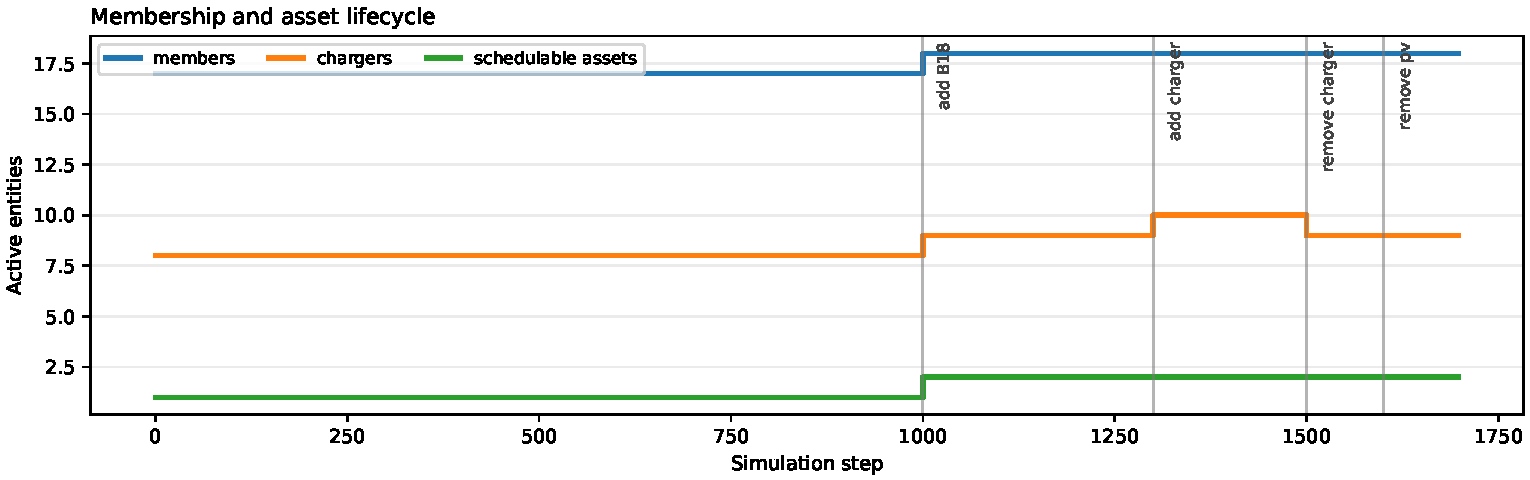
\includegraphics[width=0.96\textwidth]{simulator-dynamic-topology.pdf}
\caption{Propagation of membership and equipment events through the simulated resource collection.}
\label{fig:sim-dynamic-topology}
\label{fig:sim-topology-timeline}
\end{figure}

\begin{samepage}
Robustness requires a further experimental capability. The same \gls{rec} must be able to encounter a specified failure while retaining the underlying demand, resources, and service requests of its nominal comparison. For the example vehicle, a missing state-of-charge reading and a lost charging command are different problems: one changes the information available to decide, while the other changes the effect of the decision.\par
\end{samepage}

Failures act at different points in the same decision loop. A missing measurement changes the information supplied to a policy; a biased forecast changes an expectation; a delayed or lost command changes actuation; and unavailable equipment restricts the feasible resource set. Their effect can be expressed through separate transformations:
\begin{samepage}
\begin{equation}
\begin{aligned}
\tilde{o}_t&=\rho_o(o_t,\mathcal{E}^{o}_t,\mathcal{E}^{u}_t),&
\tilde{f}_t&=\rho_f(f_t,\mathcal{E}^{f}_t),\\
a_t^{\mathrm{cmd}}&=\rho_a(a_t^{\mathrm{req}},\mathcal{E}^{a}_t),&
a_t^{\mathrm{app}}&=\Gamma(a_t^{\mathrm{cmd}},x_t,e_t).
\end{aligned}
\label{eq:sim-robustness-channels}
\end{equation}
Here, $o_t$ and $f_t$ are nominal observations and forecasts, and their tilded forms are the values exposed after perturbation. The event sets $\mathcal{E}^{o}_t$, $\mathcal{E}^{f}_t$, $\mathcal{E}^{a}_t$, and $\mathcal{E}^{u}_t$ describe observation, forecast, command, and availability failures. Functions $\rho_o$, $\rho_f$, and $\rho_a$ apply their configured transformations. The intermediate command $a_t^{\mathrm{cmd}}$ is the request after command disturbance, while $\Gamma$ denotes the remaining action handling, including resource availability, used to obtain $a_t^{\mathrm{app}}$. These expressions identify the failure channels; their configured order is retained with the scenario.\par
\end{samepage}

Separate event streams make each failure channel an experimental variable. A missing observation can first be studied with working equipment, then combined with a lost command to examine their interaction. Noise, bias, stuck values, clipping, delay, dropout, and equipment unavailability specify different disturbances; seeds make stochastic perturbations repeatable. The nominal demand and service requests remain common to the paired runs, so changes in their outcomes can be related to the imposed disturbance.

Figure~\ref{fig:sim-robustness-channels} illustrates the resulting separation in a diagnostic run. Missing observations, forecast bias, command dropout, and equipment unavailability occupy different windows. The exported trajectory retains the nominal information, the information exposed to the controller, and the requested and applied actions. Later robustness comparisons can consequently measure service loss and recovery under a reproducible disturbance and examine which part of the control loop was affected \parencite{fonseca2026citylearnv3}.

\begin{figure}[H]
\centering
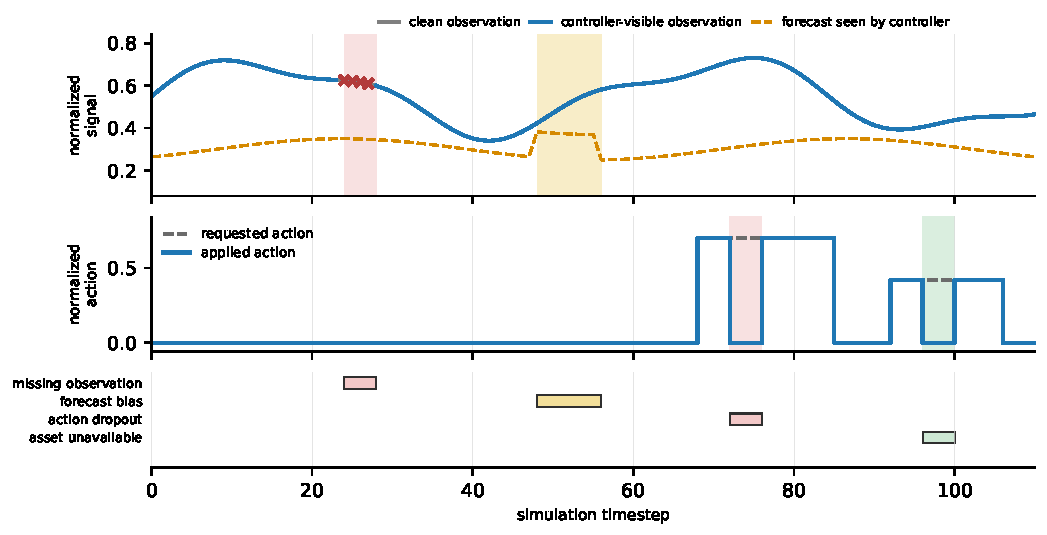
\includegraphics[width=0.96\textwidth]{simulator-robustness-channels.pdf}
\caption{Separate observation, forecast, command, and equipment-availability disturbances in the diagnostic run.}
\label{fig:sim-robustness-channels}
\end{figure}

\subsection{Controller Interfaces and Multiple Communities}
\label{sec:sim-entity}

The interaction follows the familiar reset-and-step sequence: initialise an episode, receive an observation, submit an action, and obtain the next observation, reward, and diagnostic information. A flat interface supports methods expecting fixed arrays. A structured interface organises data by entity type, identifier, relationship, availability, and action bounds. When a charger is installed, its row identifies the resource and its building instead of leaving its meaning dependent only on a vector position.

Both views use the same resource models and scenario events. This allows experiments to examine the effect of controller representation while keeping the physical setting common. Existing methods can use a compatible fixed view, while set- and graph-based methods can process active resource collections. Chapter~\ref{chap:ti-marl} develops the typed representation used for changing local interfaces. Resource identities, observation fields, and action bounds also supply the input/output description exported with the model in Chapter~\ref{chap:energAIze}, connecting simulated evaluation to deployment.

Several \glspl{rec} can be simulated together through \texttt{MultiCommunityEnv}. Each has its own scenario, buildings, controller, rewards, and outcomes, with a common clock advancing them in lockstep. Synchronised runs share the timestep, episode length, and compatible interface settings. This permits population and portfolio studies to measure local performance alongside the combined computational workload. Exchange between \glspl{rec} is a separate scenario choice; the aggregation rules in Section~\ref{sec:sim-scorecard-aggregation} combine their results without altering their physical trajectories.

\label{sec:sim-validation}
The implementation was examined through regression tests, physical and time-unit checks, controller-interface checks, and consistency checks on indicators and exports. The simulator study documents these procedures, their outcomes, and computational measurements \parencite{fonseca2026citylearnv3}; Appendix~\ref{app:simulator-audit-evidence} retains the supporting records. The figures above draw on its archived examples and show the implemented mechanisms that the datasets and controller comparisons below use.

\section{Community Datasets and Experimental Scenarios}
\label{sec:sim-annual-dataset-suite}

The datasets turn the capabilities described above into a progression of experimental settings. Small \glspl{rec} make individual decisions easy to inspect; larger \glspl{rec} introduce more resources, different daily routines, and concurrent service demands. Controlled scenario variants then change selected operating conditions. The Portugal collection follows this progression through four scenario bases and nine configurations, giving the later controller studies a common set of inputs whose purpose and assumptions are explicit.

The current edition covers 2023 and 2024 continuously at 15-minute resolution. It contains 70,176 records: 35,040 for 2023 and 35,136 for leap-year 2024. Two consecutive years provide different weather, prices, and routine realisations while preserving the \gls{rec} history. The collection is identified as \texttt{portugal-native-2023-2024-v3.1}; Appendix~\ref{app:portugal-current-audit} gives its descriptive analysis, audit results, and reproducibility record. Earlier annual experiments remain identified with their original datasets in Appendix~\ref{app:annual-suite-contract}.

\subsection{Construction and Common Assumptions}
\label{sec:sim-dataset-common-contract}

Public energy and weather sources provide the external chronology, while synthetic members and routines supply heterogeneous \gls{rec} activity. Portuguese demand statistics and E-REDES profiles inform consumption levels and shapes; household presence, opening hours, and simplified end uses introduce variation between members \parencite{dgegconsumption2023,pordataconsumption2023}. \gls{pv} production follows the site's geometry and installed equipment using the archived solar resource. \gls{omie} supplies the wholesale price chronology, and the reference tariff adds the declared variable components. Weather and carbon inputs retain their own sources and derivations, documented in Appendix~\ref{app:portugal-current-audit}.

The \gls{utc} timeline preserves elapsed time through daylight-saving changes. Civil-time fields in \texttt{Europe/Lisbon} preserve the meaning of arrivals, opening hours, holidays, and school calendars. This matters for the running example: an 08:00 departure is a local service requirement, while the energy delivered depends on the number and duration of physical intervals before it.

The second year preserves the members and equipment and continues the composition reached at the end of 2023. Permanent departures and retirements remain effective. New weather, market data, and deterministic realisations of routines supply another year of operating conditions. Sessions crossing New Year retain their continuity, so midnight does not create an artificial vehicle arrival. A simulation beginning partway through this history must initialise the corresponding topology and resource state.

Prices use one common \gls{btn} bi-hourly indexed reference across all members. The stored series contains the full variable purchase price; export to the grid is unremunerated. Local exchange is disabled in the distributed data schemas and can be enabled in the resolved experiment configuration at 80\% of the common grid-purchase price. This keeps the price convention explicit while preserving differences in the members' electrical connections and equipment.

Forecast inputs distinguish information already available from later realisations. Price forecasts use published day-ahead information when available and persistence otherwise; weather uses daily persistence. The corresponding forecast errors and publication boundary are analysed in the appendix. These simple references provide a reproducible information setting for the controller comparisons.

\subsection{Community Bases and Their Experimental Roles}
\label{sec:sim-dataset-composition}

The four bases offer different ways of examining controller behaviour. Table~\ref{tab:sim-annual-suite-composition} gives their complete inventories; the differences in ownership and activity explain the experimental role of each one.

\paragraph{Core-4: inspectable local decisions.}
Four residential members form a compact \gls{rec} with one \gls{pv} site, one stationary battery, and two charging sites. This makes it possible to follow a decision from one resource to the \gls{rec} balance. The evening charging example can be inspected alongside a neighbour's solar production or a battery schedule, and a missed departure can be traced back through the preceding actions. Core-4 is consequently useful when establishing that a controller receives the intended information and delivers the expected services before undertaking more expensive studies.

\paragraph{Core-15: residential diversity and method development.}
Fifteen households introduce more combinations of generation, charging, appliance use, and consumption-only participation. Different routines make flexibility available at different times even though the setting remains residential. This supports method development, reward and observation studies, and repeated comparisons of candidate designs at a moderate computational cost. Overlapping arrivals and appliance windows make several households compete for favourable periods. The controller must use differences in their available time while maintaining each service.

\paragraph{Core-30: mixed activity and controlled comparisons.}
Twenty-four households and six service premises extend demand and charging activity across the day. Ten \gls{pv} sites, three stationary batteries, fifteen charging connectors, and nineteen controllable appliances create concurrent decisions under finite electrical headroom. Core-30 Normal supplies the reference \gls{rec} for the Topology, Safety, Robustness, and Combined configurations. Daytime service activity changes the demand available to absorb solar production, while residential charging extends obligations into the evening. Keeping this physical base common across variants isolates the operating condition being studied.

\paragraph{Premium-100: larger and more heterogeneous communities.}
Eighty households and twenty service premises include offices, retail, clinics, cafes, workshops, and facilities with longer operating hours. The complete base contains twenty batteries and sixty-five charging connectors; one office has twelve ports. Premium Normal supports studies of larger populations and richer local interfaces, while Premium All-in combines changing participation with disturbances and demand-response services. The concentration of chargers at individual sites creates a further scheduling difficulty: several departures can compete for one building's electrical headroom. The scalability study therefore concerns both \gls{rec} size and the number of decisions within a member.

\begin{table}[!htbp]
\centering\small
\caption{Complete physical inventories in the Portugal 2023--2024 collection.}
\label{tab:sim-annual-suite-composition}
\begin{tabularx}{\textwidth}{@{}Xrrrr@{}}
\toprule
\textbf{Quantity} & \textbf{Core-4} & \textbf{Core-15} & \textbf{Core-30} & \textbf{Premium-100}\\
\midrule
Members & 4 & 15 & 30 & 100\\
\gls{pv} sites & 1 & 4 & 10 & 36\\
Stationary batteries & 1 & 1 & 3 & 20\\
Charging sites & 2 & 5 & 10 & 41\\
Charging connectors & 2 & 6 & 15 & 65\\
Vehicle identities & 2 & 6 & 19 & 85\\
Controllable appliances & 2 & 10 & 19 & 64\\
Consumption-only members & 1 & 5 & 10 & 32\\
\bottomrule
\end{tabularx}
\end{table}

Ownership overlaps across all four bases. A household may produce \gls{pv} energy without owning a battery, and a consumption-only member may benefit from energy supplied by another participant. The inventories therefore describe an uneven distribution of control opportunities. Population and composition both change between bases; experiments intended to isolate the effect of population size select matched compositions in addition to reporting the base used.

A charging site, a physical connector, a vehicle identity, and a visit remain separate quantities. The two-year static catalogues contain 9,691 sessions in Core-30 and 41,288 in Premium-100, including visits censored at the record boundaries. Residential visits include commuting, night work, and daytime presence; services introduce shorter and repeated visits. Requested departure \gls{soc} ranges from 50\% to 100\%. The catalogue therefore extends the evening-arrival example into a wider range of service windows.

Controllable appliance counts refer to physical devices. Programme profiles and requests are counted separately, while fixed appliance demand is already included in the non-shiftable load. The appendix retains both quantities, together with programme energy and the time available to schedule each request.

\begin{figure}[H]
\centering
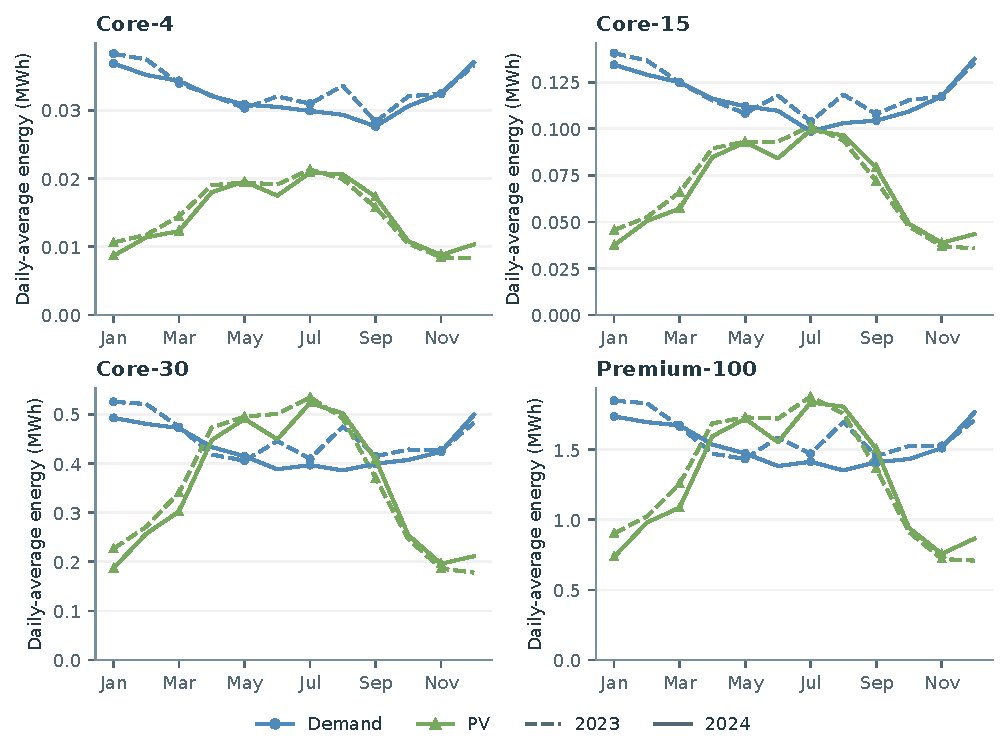
\includegraphics[width=\textwidth]{simulator-portugal-seasonal.pdf}
\caption{Monthly daily-average input demand and \gls{pv} production in the four static \gls{rec} bases.}
\label{fig:sim-dataset-profiles}
\end{figure}

Figure~\ref{fig:sim-dataset-profiles} shows the seasonal setting for these decisions. In Premium-100, non-shiftable input demand changes from 583.81 to 560.19~MWh between 2023 and 2024, and \gls{pv} production changes from 476.60 to 469.16~MWh. Within a year, the balance also changes with the season. A controller consequently encounters different opportunities for solar use even when the installed equipment is unchanged.

The daily profiles in Figure~\ref{fig:sim-dataset-daily} show the timing more directly for Core-30. The winter demand peak occurs in the evening, after \gls{pv} production has fallen, while the summer mean profile has a pronounced daytime solar surplus over non-shiftable demand. Residential vehicle presence is greatest overnight; service vehicles provide charging opportunities during the day. The controller must fit charging into these different windows while meeting departure requirements. The current connectors permit charging only, so stationary batteries provide the stored-energy flexibility between periods of production and later demand.

\begin{figure}[H]
\centering
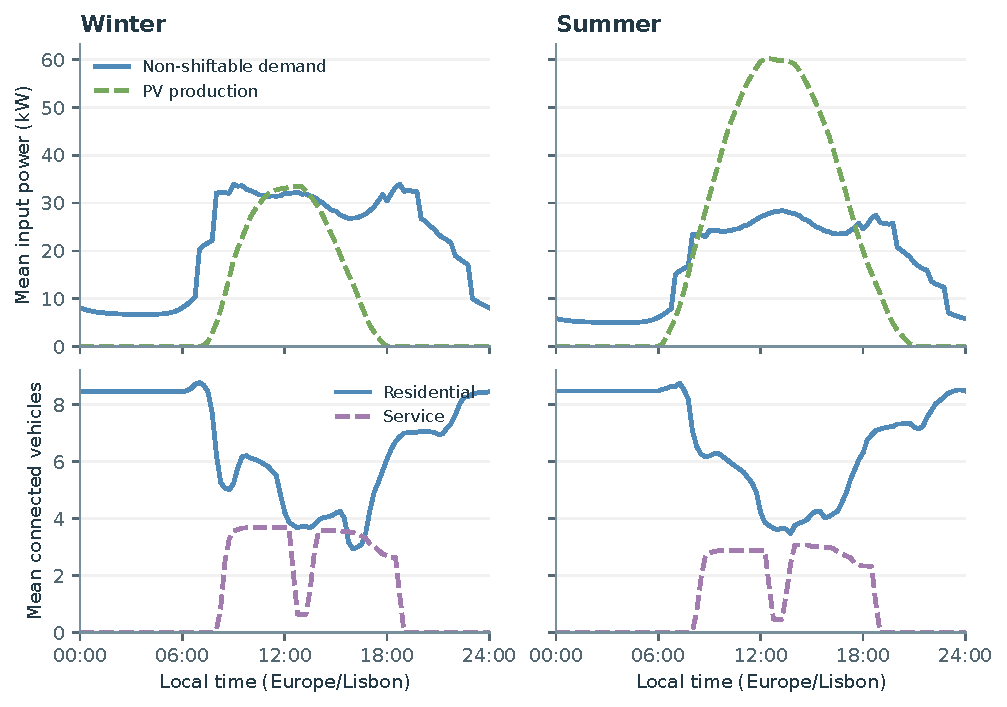
\includegraphics[width=\textwidth]{simulator-portugal-daily.pdf}
\caption{Core-30 daily input and vehicle-presence profiles: Monday--Friday means in winter (December--February) and summer (June--August) of 2024, in Lisbon local time.}
\label{fig:sim-dataset-daily}
\end{figure}

\subsection{Scenario Variants and the Questions They Address}
\label{sec:sim-dataset-variants}

The configurations distinguish the \gls{rec} being studied from the condition applied to it. The Normal cases retain the complete membership and equipment catalogue without the additional event campaigns. They establish how a controller operates with the resources, services, and electrical limits of that base. The remaining configurations make selected difficulties explicit, as summarised in Table~\ref{tab:sim-scenario-purpose}.

\begin{table}[!htbp]
\centering\small
\caption{Purpose of the scenario variants and their reference comparisons.}
\label{tab:sim-scenario-purpose}
\begin{tabularx}{\textwidth}{@{}p{0.18\textwidth}p{0.34\textwidth}X@{}}
\toprule
\textbf{Configuration} & \textbf{Change relative to its Normal base} & \textbf{Question supported}\\
\midrule
Core-30 Topology & Permanent member and equipment additions, removals, and replacements. & Can control continue as the active resource collection changes?\\
Core-30 Safety & Tighter selected building and phase limits. & Can the controller deliver services under reduced headroom, and how much action correction is needed?\\
Core-30 Robustness & Data and equipment events, observation noise, and grid interruptions. & How do disturbances affect decisions, service, and recovery?\\
Core-30 Combined & Membership changes, electrical stress, health events, and interruptions. & What happens when these conditions occur in the same \gls{rec} history?\\
Premium All-in & Participation changes, failures, interruptions, seasonal noise, and demand-response requests. & How does control perform when a larger, heterogeneous \gls{rec} faces several operating demands?\\
\bottomrule
\end{tabularx}
\end{table}

Safety changes the headroom against which actions are evaluated, making service delivery and reliance on limiting central to the comparison. Robustness retains a reproducible failure schedule, allowing nominal and disturbed trajectories to be compared through the affected services and recovery period. Topology changes which members and assets are active. These configurations give the corresponding \glspl{rq} concrete experimental contrasts. Combined and All-in then examine their interaction within an integrated workload; paired diagnostic replays can distinguish individual effects when needed.

The topology histories describe permanent participation changes. Core-30 Topology and Combined begin with 26 active members and finish with 27; Premium All-in begins with 80 and finishes with 88. The full catalogues contain the resources available to those histories. Events also install, replace, or retire equipment. A member that leaves exits subsequent \gls{rec} demand and service accounting, and the same departure is not replayed in 2024.

Failure events and observation noise remain separate scenario settings. The former specify intervals of missing data, forecast bias, delayed or lost commands, and equipment unavailability. Core-30 Robustness additionally includes its continuous measurement-noise setting, while Premium All-in uses seasonal noise campaigns. Backup during grid interruptions follows the aggregate convention supported by the selected runtime. The timing and intensity of these conditions remain explicit, allowing service loss and recovery to be evaluated against matched nominal operation.

\gls{dr} appears only in Premium All-in. Each year includes two one-hour reduction requests of 80~kW and one one-hour absorption request of 40~kW, together with a separately identified four-hour reduction request of 1500~kW. The last is a deliberately excessive request used to examine behaviour under unattainable service demand. Its outcome belongs to a separate stress category from the operational candidate requests.

Development and reserved confirmation files select different event schedules within these configurations. A paired comparison retains the physical inputs and declares the event or operating condition changed. The two-year chronology also permits temporal separation, with training, selection, and confirmation windows specified by each controller study. Initialisation preserves the \gls{rec} history at the selected start time, so a member that departed earlier remains absent.

\subsection{Data Characterisation and Quality}
\label{sec:sim-annual-baseline-audit}

The dataset analysis follows the same distinctions used in construction: installed and active resources, input energy and controlled energy, scheduled visits and delivered charging, and requested services and completed services. Appendix~\ref{app:portugal-current-audit} develops that analysis through distributions, temporal profiles, and event summaries. It also records the checks supporting the current edition.

The input checks cover the time axis, calendar, inventories, resource identities, connection schedules, appliance windows, forecasts, and event histories. Individual charging requests are also examined against their connection duration, accepted power, losses, and battery taper. The resulting audit accompanies the descriptive analysis in the appendix. Concurrent demand, electrical limits, disturbances, and the controller's decisions then determine which services are delivered during simulation.

The archived examples in Section~\ref{sec:sim-architecture} illustrate the implemented mechanisms. The Portugal collection supplies the inputs for the controller comparisons that follow, with its descriptive analysis and audit retained together in the appendix.

\section{Performance Indicators and Evaluation Protocol}
\label{sec:sim-evaluation}

The value of a control decision depends on the service it delivers and the resources it uses. Returning to the example vehicle, a lower electricity bill is useful when the vehicle is ready at 08:00 and the charging schedule respects the installation limits. A \gls{rec} assessment must also show whether the gain is shared among its members and how the controller behaves when conditions change. The evaluation therefore reads energy and economic outcomes together with service, safety, robustness, and computational effort.

The simulator extends the inherited energy indicators with participant services, local settlement, electrical constraints, and operating events. The definitions below establish the common scorecard and comparison rules used in the following chapters. Scenario choice determines the members, resources, prices, and active services; Chapters~\ref{chap:control-benchmark} and~\ref{chap:ti-marl} specify the learning methods, training budgets, data windows, seeds, and ablations. Each result is thus read against the same definitions while retaining the conditions of its experiment.

\subsection{Energy, Cost, and Community Outcomes}

Grid import and export record how much energy crosses the selected building or \gls{rec} boundary. Their difference is net exchange, but the two directions remain available separately: identical net totals can arise from very different patterns of consumption and surplus. Local sharing records which part of member demand is met within the \gls{rec} and how the associated payments are allocated. The accounting boundary and settlement settings are consequently part of every comparison.

For a matched reference controller, cost saving is
\begin{samepage}
\begin{equation}
\Delta C=C_{\mathrm{ref}}-C_{\pi}.
\label{eq:sim-cost-saving}
\end{equation}
Here, $C_{\pi}$ is the cost of the evaluated policy $\pi$, and $C_{\mathrm{ref}}$ is reference cost over the same members, intervals, prices, and settlement rules. The saving $\Delta C$ is expressed in currency and is positive when the evaluated policy reduces cost. Demand-response payments and penalties remain identifiable within the reported cost after settlement. Absolute savings also remain interpretable when the reference cost is zero or negative.\par
\end{samepage}

Participant outcomes extend this reading beyond the \gls{rec} sum. The savings count includes members active in the scored period with finite costs in both runs; a member saves when its cost difference is positive. The scorecard gives this count, its percentage of eligible members, and the distribution of absolute savings. Percentage cost reductions additionally require a positive reference cost. In a changing \gls{rec}, each member is compared over its active period. Figure~\ref{fig:sim-rec-settlement} shows why this matters: the same sharing mechanism produces different benefits for members with different generation and demand.

Solar self-consumption relates generation to the amount retained within the stated accounting boundary:
\begin{samepage}
\begin{equation}
S_{\mathrm{PV}}=100\frac{G-X_{\mathrm{PV}}}{G},\qquad G>0.
\label{eq:sim-solar-use}
\end{equation}
Here, $G$ is total \gls{pv} generation and $X_{\mathrm{PV}}$ is the energy attributed to \gls{pv} export at that boundary, both in kWh. The indicator $S_{\mathrm{PV}}$ is a percentage; it is undefined when there is no generation. Building and \gls{rec} values refer to different boundaries, since energy exported by one member may be consumed by another. The source totals accompany the ratio so that the level of aggregation remains clear.\par
\end{samepage}

Battery throughput sums the charging and discharging energy of stationary batteries at the declared metering boundary, in kWh. \gls{v2g} export separately totals the energy supplied by vehicle batteries, also in kWh. Their interpretation depends on the cost, service, and grid outcomes achieved, together with any degradation model included in the experiment. A larger throughput can accompany useful solar shifting or unnecessary cycling; its magnitude explains resource use without supplying an independent ranking.

Operational emissions accumulate imported electricity multiplied by the corresponding interval carbon intensity, giving kg~CO$_2$. The report identifies whether imports are measured at individual member meters or after \gls{rec} balancing, and uses the same boundary for all methods. Any export credit follows an explicitly declared accounting rule. These quantities allow two equally inexpensive schedules to be distinguished by renewable utilisation, storage use, or emissions.

The grid-shape indicators use \gls{rec} net power, positive for import. The all-time peak is its maximum over the scored period. Daily peak is the mean of the maxima in successive 24-hour windows from the episode start; at 15-minute resolution, each complete window contains 96 intervals. A final partial window is included when present. The daily load-factor penalty averages one minus the ratio of mean to maximum power in those windows. Raw peaks are in kW, while the load-factor penalty is dimensionless. The scorecard reports both peaks in kW; the load-factor penalty remains available in the wider catalogue.

Ramping uses the sum of positive changes in \gls{rec} net power between consecutive intervals, including intervals of net export. It therefore measures upward changes, such as the rise when evening charging begins as solar production falls. The scorecard reports this accumulated upward change in kW over the complete evaluation window. It is a sum of power increments, rather than a rate in kW per hour. These conventions follow the simulator's power-based comparison outputs. Legacy indicators calculated from interval energy retain their separate units; comparisons use the same resolution and convention throughout.

\subsection{Service Delivery, Safety, and Robustness}
\label{sec:sim-service-evaluation}

Vehicle service is evaluated at departure with a tolerance of five percentage points of \gls{soc}. Minimum acceptable service is reached at or above the requested target minus this tolerance. Target accuracy requires the final state to lie within five percentage points on either side of the target. For an 80\% request, minimum service begins at 75\%, while the accuracy band is 75--85\%. The corresponding rates are
\begin{samepage}
\begin{equation}
S_{\min}=100\frac{N_{\min}^{\mathrm{met}}}{N_{\min}^{\mathrm{eligible}}},\qquad
S_{\mathrm{tol}}=100\frac{N_{\mathrm{tol}}^{\mathrm{met}}}{N_{\mathrm{tol}}^{\mathrm{eligible}}}.
\label{eq:sim-service-rates}
\end{equation}
Here, $S_{\min}$ and $S_{\mathrm{tol}}$ are the minimum-service and within-tolerance percentages. For each criterion, $N^{\mathrm{eligible}}$ counts eligible departures and $N^{\mathrm{met}}$ counts those meeting the criterion. A rate is undefined when its eligible count is zero. The counts and the number of excluded departures accompany both percentages.\par
\end{samepage}

An eligible departure has an observed session end, a valid target and achieved \gls{soc}, and a threshold reachable under the simulator's maximum-charge feasibility screen. This screen starts from the session boundary state and follows the available connection intervals, charger and battery power limits, efficiencies, and battery taper. It applies the configured electrical headroom and outage handling. Eligibility is calculated for each threshold, independently of whether the controller meets it. The common five-point tolerances give both criteria the same lower threshold; their success counts differ when charging exceeds the upper accuracy limit. Individually unattainable requests remain visible alongside the eligible results.

The service record gives failed departures as a count over eligible departures and reports both the total and largest individual energy deficit. For each eligible departure, the deficit is the positive difference between the battery energy required at the minimum-service threshold and the energy present at departure, in kWh. This distinguishes many small shortfalls from a few severely underserved vehicles. Energy missing from the original requested target remains a separate diagnostic, since the minimum-service criterion includes the stated tolerance. Unattainable requests and exclusions caused by missing or incomplete records retain separate counts. A paired disturbance comparison also identifies departures that lose eligibility and reports service on the common eligible cohort, so that an outage cannot improve the apparent rate simply by removing difficult requests.

Appliance service is read through completed and missed cycles, completion deadlines, start delay, delivered energy, and unserved energy. A shifted washing programme can then be distinguished from a programme that never ran. Demand-response records likewise retain requested and credited response, shortfall, compliance, and settlement for each activation. These service quantities remain visible beside energy savings, including in Combined and All-in scenarios where several obligations compete for the same flexibility.

Electrical safety is measured on the applied trajectory, while requested pressure describes the actions proposed before limiting. Accumulated exceedance can be written as
\begin{samepage}
\begin{equation}
V=\frac{\Delta t}{3600}\sum_{t\in\mathcal{T}}\sum_{\ell\in\mathcal{L}_t}
\left([P_{\ell,t}-I_{\ell}^{\max}]_+ +[-P_{\ell,t}-X_{\ell}^{\max}]_+\right).
\label{eq:sim-violation-energy}
\end{equation}
Here, $\mathcal{T}$ contains the scored timesteps and $\mathcal{L}_t$ the configured total-building and phase boundaries active at timestep $t$. Applied power $P_{\ell,t}$ is positive for import; $I_{\ell}^{\max}$ and $X_{\ell}^{\max}$ are positive import and export limits, all in kW. The notation $[z]_+=\max(z,0)$ retains positive excess, and $\Delta t$ is the timestep in seconds. Thus, $V$ measures accumulated constraint exceedance in kWh, counting each violated total or phase limit. The residual calculation uses a numerical tolerance of $10^{-5}$~kW.\par
\end{samepage}

The frequency of actual action corrections accompanies this applied safety result:
\begin{samepage}
\begin{equation}
 A_{\mathrm{corr}}=100\frac{N_{\mathrm{corr}}}{N_{\mathrm{decision}}}.
 \label{eq:sim-action-correction}
\end{equation}
Here, $N_{\mathrm{decision}}$ counts eligible building-level decision opportunities with an active controllable resource and a supplied proposal. The numerator $N_{\mathrm{corr}}$ counts those opportunities in which at least one command is actually changed by the declared feasibility or supervisory stages. The rate $A_{\mathrm{corr}}$ is a percentage, with a stated numerical tolerance for detecting changes. Each building decision is counted once even if several commands or stages change it.\par
\end{samepage}

A call to a validator with an unchanged output adds no correction. Missing, invalid, or late decisions are counted once per building decision opportunity when a usable action is unavailable by the declared control deadline. Their denominator includes all opportunities requiring a decision, including those with no proposal. This differs from the correction denominator, which requires a supplied proposal. The report names the stages included and preserves proposed, submitted, and applied actions, following Section~\ref{sec:sim-contracts}.

Fallback records describe the supervisor's response. An episode is a consecutive period of fallback within one building; separate buildings contribute separate episodes. Total duration is summed in building-minutes, with overlapping periods therefore retained for each affected building. Per-resource corrections and their magnitude remain available for diagnosis. A corrected command or a fallback decision can preserve the requested service, so intervention and missed service keep separate counts. Injected fault episodes and their duration describe exposure to the disturbance and are recorded independently of these outcomes.

Robustness uses the same outcomes in paired nominal and disturbed runs. The comparison fixes the underlying scenario, controller, and random seeds and changes the selected disturbance. It reports energy and cost differences, missed or delayed services, and action correction during the event and afterwards. Execution recovery is measured from clearance of the declared external fault to the first usable controller decision applied within its deadline. Median and maximum recovery time accompany the number of recovered and unrecovered episodes. Episodes still unresolved at the observation boundary retain their elapsed duration as a lower bound. Service recovery is reported separately where an obligation can still be fulfilled; a missed departure remains a missed service even after timely execution resumes.

\subsection{Scorecard, References, and Aggregation}
\label{sec:sim-scorecard-aggregation}

The simulator provides a much wider set of performance indicators than can be usefully displayed in every comparison. Member savings use matched \gls{bau} operation as a reference, with its storage variants defined in Chapter~\ref{chap:control-benchmark}. The common scorecard in Table~\ref{tab:sim-core-scorecard} selects fifteen indicators that keep the results aligned across methods, datasets, and chapters. It gives an economic outcome its energy, service, and operational context. The wider catalogue in Appendix~\ref{app:sim-kpi-catalogue} remains available for questions about appliance service, local settlement, \gls{dr}, topology, failures, comfort, degradation, and multi-\gls{rec} operation.

\begin{table}[!htbp]
\centering
\caption{Common scorecard. Physical and monetary quantities retain their absolute units; percentages describe service, utilisation, or intervention directly.}
\label{tab:sim-core-scorecard}
\footnotesize
\setlength{\tabcolsep}{4pt}
\renewcommand{\arraystretch}{1.16}
\begin{tabularx}{\textwidth}{@{}>{\raggedright\arraybackslash}p{0.16\textwidth}>{\raggedright\arraybackslash}X >{\raggedright\arraybackslash}p{0.25\textwidth}@{}}
\toprule
\textbf{Category} & \textbf{Indicators and units} & \textbf{Reading} \\
\midrule
Economy & \gls{rec} cost [EUR]. & Lower, with service retained. \\
Emissions & Operational emissions [kg CO$_2$]. & Lower under the same accounting rule. \\
Energy & External \gls{rec} import [kWh]; external \gls{rec} export [kWh]; solar self-consumption [\%]. & Read the two exchange directions with local solar use. \\
Grid shape & Mean daily peak [kW]; maximum peak [kW]; accumulated upward ramping [kW]. & Lower under matched service and timestep. \\
\gls{ev} service & Minimum service [\%]; target accuracy [\%, $\pm5$ \gls{soc} percentage points]. & Retain the eligible and excluded departure counts. \\
Safety and supervision & Electrical violations [kWh]; actual action corrections [\% of eligible building decisions]. & Zero residual violation; interpret correction with delivered service. \\
Resource use & Stationary-battery throughput [kWh]; \gls{v2g} export [kWh]. & Explain how flexibility was used. \\
Member benefit & Members saving against matched \gls{bau} [$n/N$]. & Show the distribution of \gls{rec} benefit. \\
\bottomrule
\end{tabularx}
\end{table}

Results use the same names and units throughout the thesis. Cost is the \gls{rec} total under the declared tariff and settlement convention; savings in EUR may accompany it. Grid import and export are measured at the \gls{rec} boundary, while the sum of member-meter imports is retained separately where useful. Service and self-consumption percentages keep their direct meaning: they express fulfilled departures or retained generation, rather than normalisation against another controller. The principal tables report cost, energy, emissions, and power in absolute units. Reference differences support interpretation without replacing those quantities.

The common operating reference uses ordinary vehicle charging, execution of mandatory appliance requests, and simple \gls{pv} self-consumption storage. A no-storage variant isolates the contribution of enabling that resource. Progressively informed \glspl{rbc} use prices, generation, peaks, and \gls{rec} information. Chapter~\ref{chap:control-benchmark} develops these references alongside optimisation and learning. Member benefit uses the matched storage-enabled \gls{bau} unless another reference is explicitly named; an incremental hierarchy comparison can additionally report savings against the same local controller without coordination.

The scorecard can be presented in two blocks with the same method order: economy, emissions, energy, and grid shape first; service, safety, resource use, and member benefit second. A focused comparison can select the methods and columns relevant to its question. A charging study, for example, may place cost beside the two \gls{ev}-service rates and intervention, while a coordination study also needs the \gls{rec} power profile and member outcomes. Safety and disturbance studies add a compact service-and-event table: failed obligations, their energy deficit, unavailable decisions, fallback, and recovery. Each table retains its dataset, complete evaluation window, and indicator definitions, allowing the comparisons to accumulate as the methods are introduced.

Additional indicators follow the services present in the experiment. A dataset containing deferrable appliances requires completion and missed-deadline outcomes beside the energy comparison; demand-response experiments retain delivered response, shortfall, and settlement. A disabled service is identified as such. Unavailable measurements remain marked as unavailable, rather than filled with a favourable zero. Export and battery throughput are diagnostic quantities, and a high value alone does not establish better control.

These observations connect directly to the four research dimensions established in Chapter~\ref{chap:introduction}. \emph{Scalability} follows control quality as the number of members and resources grows, together with training time [h], peak memory [GB], and inference latency [ms per building decision]. It also records the preparation or retraining needed after a configuration change. \emph{Deployability} concerns the work needed to place the controller in service: configuration and integration effort [person-hours], elapsed deployment time, runtime dependencies, and the successful reproduction of the evaluated decisions through the deployed inference path. Those measurements accompany the scorecard in the corresponding studies.

\emph{Safety} is read through service fulfilment, physical violations, and the interventions supporting the applied decisions. \emph{Robustness} uses the same outcomes in paired nominal and disturbed conditions, supplemented by fallback and service-specific recovery times. The common scorecard thus supplies a stable account of useful operation, while each investigation adds the observations needed to examine its \gls{rq}. Keeping these meanings stable allows the architecture, simulation, and learning studies to contribute to the same argument.

Aggregation follows the measured quantity. Cost sums the member bills under the selected settlement rule; internal payments cancel in the \gls{rec} total when transfers between members are represented. Energy and emissions accumulate over the scored intervals at their declared boundary. Solar self-consumption is calculated from total generation and \gls{pv}-attributed export, rather than the unweighted mean of building percentages. Maximum peak is taken from the aggregate \gls{rec} trajectory, mean daily peak averages its daily maxima, and ramping accumulates its successive positive power changes. None of these power quantities is obtained by summing independently computed building peaks.

Service rates pool the corresponding met and eligible event counts, and correction rates pool corrected and eligible building decisions. Their denominators and exclusions remain visible. Member benefit counts matched active members with finite bills and retains the range of absolute savings in the detailed results. Each dataset is reported separately. Where repeated training runs are available, each run first yields a scorecard for the full test window; the report then gives the mean and dispersion across independent training seeds, retaining paired simulator conditions for each comparison.

\subsection{Temporal Protocol and Reproducible Comparisons}
\label{sec:sim-temporal-protocol}

The two-year Portugal collection separates controller development from operation on a later annual sequence. The studies in Chapter~\ref{chap:control-benchmark} use 2023 for training and validation and reserve the complete available 2024 sequence for final evaluation. A full year exposes a controller to changing demand, solar production, prices, and service requirements across the seasons. Short event plots explain particular decisions within that annual account.

Training allows the agent to interact with the simulator and improve its policy. Validation evaluates selected policies on reserved periods to choose hyperparameters, reward settings, and checkpoints. Four fortnightly blocks---the first fourteen days of February, May, August, and November 2023---provide validation conditions in different seasons. The remaining 2023 intervals supply training episodes. Table~\ref{tab:sim-temporal-split} identifies the role of each partition.

\begin{table}[htbp]
\centering\small
\caption{Temporal separation for the principal controller comparisons.}
\label{tab:sim-temporal-split}
\begin{tabularx}{\textwidth}{@{}p{0.17\textwidth}p{0.33\textwidth}X@{}}
\toprule
\textbf{Stage} & \textbf{Data window} & \textbf{Use}\\
\midrule
Training & 2023, excluding the four reserved validation blocks. & Generate interaction experience, update the policy, and fit preprocessing statistics.\\
\addlinespace
Validation & Days 1--14 of February, May, August, and November 2023. & Compare configurations and select checkpoints with learning disabled.\\
\addlinespace
Final test & Complete available 2024 sequence. & Evaluate the selected policy with its parameters, preprocessing, and action-selection rule fixed.\\
\bottomrule
\end{tabularx}
\end{table}

The split follows the dataset's \gls{utc} clock. Training episodes retain contiguous time intervals; replay records and learning targets stop at the partition boundaries. Validation observations and rewards do not enter policy updates or the fitting of preprocessing statistics. Initialisation reconstructs the active resources and relevant preceding history at each episode's start, with any warm-up kept outside the score. The continuous test year then carries stored energy and unfinished services forward without daily or monthly resets.

\gls{bau} and fixed rule-based references use the same annual test window as the learned controllers. \gls{bau} can also be evaluated over the full development year to characterise conventional operation, with 2023 and 2024 reported separately. The primary comparison pairs each controller with its reference within the same scenario and year. The seven Core-30 and Premium-100 scenarios provide this principal account; Core-4 and Core-15 support development and diagnostic inspection. Comparisons across \gls{rec} sizes additionally retain their different resource compositions.

Candidate and reference share the dataset edition, active members and resources, physical inputs, service requests, prices, settlement, electrical limits, events, timestep, and scored interval list. Initial stored energy, preceding \gls{rec} history, and the handling of services crossing either boundary are also matched. Changes of membership follow the same event schedule for all methods. The record gives the first and last scored action timestamps and the executed interval count; warm-up observations and an unexecuted terminal observation contribute no artificial energy or cost. Near-boundary forecast handling follows the same convention across the comparison.

The selected checkpoint and preprocessing statistics are frozen for evaluation. A study of online adaptation declares its update rule separately and compares it under the same test conditions. Repeated training seeds reveal variation in the learned solution, while paired simulator seeds retain common disturbances for candidate and reference. Episode segmentation preserves resource state and unfinished services across the full test sequence unless resets are themselves part of the declared experiment. This prevents a series of freshly initialised short episodes from silently replacing continuous operation.

Information access and protective settings accompany each result. Local and \gls{rec}-aware methods retain their declared observation boundaries, and forecasts use the same availability convention. A perfect-information schedule is reported separately as an opportunity reference. An optimisation method evaluated through successive horizons still covers the complete test sequence, carrying state and unfinished obligations between horizons. A short mathematical solve remains a diagnostic with its own scope; simulator replay supplies the operating outcomes needed for the common scorecard.

Disturbance studies retain complete-window outcomes as well as the intervals around each event. They fix the underlying scenario, controller, and paired random conditions, then change the declared disturbance. Additional energy, missed service, intervention, and recovery can consequently be attributed to that change. Demand-response assessment likewise retains the reference estimator, credited response, penalties, and cost after settlement. A no-activation replay with the same policy measures additional response, while subsequent intervals reveal rebound and differences in stored energy. Operational candidate requests and deliberately excessive stress requests retain separate categories.

Computational comparisons identify the hardware, software, population, resource counts, observation/action sizes, interaction budget, and update budget. Training time and memory describe development; inference measurements report the declared timing boundary, batch size, warm-up, and latency distribution. The 95th-percentile latency describes the slower part of that distribution, while late decisions are counted against the actual control deadline over the complete test window. The timing boundary states whether observation preparation, inference, validation, and dispatch are included. A change of resources additionally records model reuse, rebuilding, retuning or retraining, and the associated interruption and service outcomes.

Deployment records separate person-hours of configuration and integration from elapsed time between the start of installation and the first valid applied decision. They retain the supporting services, resource mapping, preprocessing, and controller composition placed in operation. Reproduction of the evaluated behaviour is checked by replaying the same recorded inputs through the packaged controller and counting matching requested actions within a declared tolerance. Timing compliance and successful dispatch are then assessed on the complete execution path. These measurements accompany the operating scorecard and explain how readily a useful controller can be placed in service.

The experiment record preserves the data, software, controller version, evaluation conditions, and resulting trajectories through the lifecycle described in Chapter~\ref{chap:energAIze}.

\section{Chapter Summary}
\label{sec:sim-discussion}
\label{sec:sim-open}

The simulator development provides the experimental setting needed to investigate \gls{rec} control under the conditions established in the opening chapters. CityLearn v3 connects resource models and participant services to electrical limits, changing membership, local exchange, external requests, and failures. The implemented examples show how these conditions enter the simulation and remain visible in observations, actions, and outcomes. Their incorporation into the official CityLearn distribution makes the capabilities available as a reusable research contribution.

The Portugal datasets organise those capabilities into an experimental progression, from inspectable residential decisions to larger \glspl{rec} with mixed activities and interacting events. Their documented inputs and scenario purposes support matched comparisons, while the performance indicators connect energy and economic outcomes to services, constraints, participant benefits, and computational effort.

This foundation makes scalability, safety, and robustness accessible to controlled experiments through changes in resources, electrical headroom, and operating conditions. It supports deployability through the consistent resource and action descriptions carried into the architecture of Chapter~\ref{chap:energAIze}. Chapter~\ref{chap:control-benchmark} now uses the simulator, datasets, and common evaluation rules to develop and compare the control methods.
\endgroup

\chapter{Progressive Control and Learning Solutions for Renewable Energy Communities}
\label{chap:control-benchmark}
\markboth{Progressive Control and Learning}{Progressive Control and Learning}

The common simulation and evaluation substrate supports a cumulative sequence of control studies. Passive operation and progressive RBCs establish feasibility and transparent operating logic; optimisation makes objectives and constraints auditable; single-agent learning introduces adaptation; MADDPG introduces decentralised coordination; MATD3 improves the deterministic multi-agent actor--critic baseline; and data-efficient and hierarchical mechanisms address reuse, sample efficiency, and local--community coordination.

The sequence begins with passive operation and rule-based control, where feasibility and transparent operating logic can be checked directly. It then introduces explicit optimisation, which makes objectives and constraints auditable. Single-agent reinforcement learning adds adaptation without requiring a complete model at every decision step. MADDPG adds decentralised multi-agent coordination, and MATD3 addresses part of the training instability and value overestimation observed with deterministic multi-agent actor--critic learning. Behaviour cloning, guided exploration, replay selection, offline learning, distillation, and hierarchical coordination then address sample efficiency, reuse, and the separation between local and community decisions.

Each stage produces a distinct empirical contribution by establishing what can be achieved, under which information and operational assumptions, and at what computational cost. The accumulated evidence also exposes the remaining integration problem: stable, data-efficient, or hierarchical controllers can still depend on fixed observation and action interfaces and on manually maintained physical contracts. Those residual assumptions become the design requirements for TI-MARL.

\draftnote{This chapter is a complete narrative and experimental blueprint. The implemented stack includes passive operation, five RBC levels, MILP, PPO, SAC, TD3, MADDPG, MATD3, RBC-guided exploration, behaviour cloning, prioritised replay, offline RL, distillation, and hierarchical coordination. Exact controller names, observation and action definitions, reward variants, training budgets, seed counts, hyperparameters, and quantitative findings must be imported from the frozen repositories and experiment store. The chapter deliberately distinguishes completed capabilities from claims that still require a final evidence audit.}

\section{Research Progression and Common Evaluation Protocol}
\label{sec:control-progression}

A controller can appear better simply because it receives more information, uses a more favourable forecast, or is evaluated on an easier scenario. To prevent this, the methods in this chapter are compared through common physical scenarios and explicit information assumptions. Loads, photovoltaic production, assets, tariffs, deadlines, constraints, and evaluation periods are shared whenever the comparison permits it. Controller-specific models or preprocessing are treated as part of the method and are reported rather than hidden.

The progression is evaluated through four recurring questions:

\begin{enumerate}
  \item \textbf{What problem was the method introduced to solve?}
  \item \textbf{What did the experiments show that it actually solved?}
  \item \textbf{Under which information, scale, and operational assumptions was that result obtained?}
  \item \textbf{What limitation remained and motivated the next step?}
\end{enumerate}

The methods are classified by their role as strong baselines, reusable mechanisms, empirical contributions, or components of TI-MARL. The recurring analysis records the problem addressed, measured result, scope, and remaining assumption for each stage.

\Cref{fig:control-progression} summarises the cumulative research progression: each stage resolves a concrete problem, retains a useful capability, and reveals the assumption addressed by the next stage.

\plannedfigure[0.16\textheight]{fig:control-progression}{Cumulative progression from explicit control to adaptive and hierarchical multi-agent coordination.}{\textbf{Type:} left-to-right progression diagram. For each stage (passive/RBC, MILP, single-agent RL, MADDPG, MATD3, learning-efficiency mechanisms, hierarchy), state the problem addressed, capability gained, and assumption left unresolved. End with the design requirements passed to TI-MARL. \textbf{Purpose:} show that earlier methods solved problems rather than merely failing before the final method. \textbf{Source needed:} final method/claim/evidence ledger.}

\paragraph{Problem instances.}
The experiments cover related levels of control rather than one universal decision problem.

\begin{description}
  \item[Asset level.] A controller schedules charging, discharging, thermal operation, or a deferrable request for one asset.
  \item[Building level.] A controller coordinates the assets behind one meter while respecting local service and electrical limits.
  \item[Community level.] A controller coordinates several buildings or modifies a shared signal to reduce cost, peak demand, ramping, emissions, or grid stress.
  \item[Reconfigurable level.] Agents, assets, capabilities, observations, actions, or topology change. This level motivates and is evaluated in \cref{chap:ti-marl}.
\end{description}

A real deployment can combine all four. For example, a community-level coordinator can issue one price multiplier, while each building continues to schedule its own EV and battery. The high-level problem and the local problem should therefore not be collapsed into one large vector merely because that is convenient for an algorithm.

\paragraph{Comparison principles.}
The evaluation follows six principles.

\paragraph{Information fairness.} Every result states what the method knew at decision time. A perfect-information MILP is an oracle reference, not an operational competitor to a policy that sees only current observations and forecasts.

\paragraph{Strong baselines.} The RBCs become progressively more informed. The optimisation formulation includes the relevant constraints. Learning methods are compared with tuned and credible alternatives, not with deliberately weak references.

\paragraph{Repeated learning runs.} RL and MARL results are reported over independent seeds. Central tendency, dispersion, learning stability, and checkpoint selection are part of the result.

\paragraph{Multiple outcomes.} Aggregate reward is not sufficient. Energy, service, safety, fairness, learning, computation, and communication metrics are reported separately before any combined score is considered.

\paragraph{Operational interpretation.} Training cost, inference latency, memory, communication, model requirements, and integration effort are considered together with energy performance.

\paragraph{Negative and boundary results.} A method that does not improve one dimension, or improves it only under a narrow assumption, remains informative. Such results define where the method should and should not be used.

\begin{table}[htbp]
\centering
\caption{Metric families used throughout the controller progression.}
\label{tab:controller-metrics}
\begin{tabularx}{\textwidth}{@{}p{0.23\textwidth}X@{}}
\toprule
\textbf{Metric family} & \textbf{Representative measures} \\
\midrule
Participant outcomes & electricity cost, grid import/export, self-consumption, comfort or departure service, asset cycling \\
Community outcomes & aggregate cost, peak demand, load factor, ramping, local renewable use, carbon indicators, demand-response delivery \\
Safety and service & infeasible proposals, clipping or projection, power-limit violations, missed EV departure targets, incomplete services \\
Learning behaviour & return, convergence, variance across seeds, sample efficiency, critic disagreement, overestimation diagnostics \\
Computational cost & training wall time, environment interactions, CPU/GPU time, memory, checkpoint size, inference latency \\
Distribution and fairness & outcome by participant and asset group, worst-participant result, dispersion of savings \\
Operational complexity & model and forecast requirements, configuration effort, communication, package size, target compatibility \\
\bottomrule
\end{tabularx}
\end{table}

\Cref{fig:control-common-protocol} defines the common protocol required for a fair comparison across controller families with different information and training requirements.

\plannedfigure[0.15\textheight]{fig:control-common-protocol}{Common experimental protocol used to compare controller families.}{\textbf{Type:} protocol schematic or experiment matrix. Show shared scenario/data split, information available to each controller, training budget, repeated seeds, evaluation episodes, KPIs, constraint metrics, computation/resource metrics, and statistical comparison. Mark perfect-information/oracle variants separately from operational-information variants. \textbf{Purpose:} make fairness of the comparisons visible before results are presented. \textbf{Source needed:} frozen protocol and configuration manifest.}

\section{Operationally Plausible and Constraint-Aware Control}
\label{sec:rbc-ladder}

\paragraph{Passive operation.}
The passive or business-as-usual case follows the native asset or user schedule without active flexibility management. An EV can begin charging when it is connected, a battery can remain idle, and a deferrable request can follow its default start. This case is not a weak controller. It is the denominator that shows how much value is created by any intervention at all.

\paragraph{Progressive rule-based controllers.}
The five RBC levels form a ladder of increasing knowledge and coordination. Their repository class names are mapped to the following conceptual levels so that the comparison remains stable across implementation revisions.

\begin{description}
  \item[Local feasibility.] The controller blocks impossible actions, remains inside asset limits, and prioritises urgent service requirements.
  \item[Time- and price-aware control.] The controller uses tariff periods, time to deadline, and threshold logic.
  \item[Forecast- and flexibility-aware control.] The controller uses short-horizon forecasts and explicit flexibility quantities, such as remaining EV energy divided by remaining connection time.
  \item[Community-aware control.] Local rules respond to community demand, headroom, or a shared coordination signal.
  \item[Expert and fail-safe control.] The strongest rule set combines local feasibility, forecasts, community context, and conservative fallback behaviour. It can also generate expert demonstrations.
\end{description}

The RBC ladder solves several problems early in the thesis. It establishes physically plausible behaviour, gives the simulator and action adapters a deterministic reference, provides a low-cost runtime fallback, and separates the value of richer information from the value of learning. If a learned controller only outperforms a local rule but not a community-aware rule, the observed gain may come from coordination information rather than from the learning mechanism itself.

The remaining limitation is adaptation. Rules can be effective when the expected conditions are known, but they need manual redesign when objectives, tariffs, asset combinations, or patterns of uncertainty change. The more conditions the rule set covers, the more difficult it becomes to reason about conflicts and maintenance.

\paragraph{Evidence from the RBC progression.}
The RBC comparison follows the complete ladder instead of reporting only the strongest rule set. Performance changes are attributed to local feasibility, temporal or forecast context, community information, and expert fallback behaviour. This creates an interpretable path from passive operation to the rule-based teacher retained by TI-MARL.

\paragraph{Explicit constraint-aware coordination.}
\label{sec:milp-control}

MILP provides a different form of intelligence. Instead of learning from repeated interaction, it represents decisions, objectives, and constraints explicitly. Binary variables can represent service activation or mutually exclusive modes; continuous variables can represent power and energy; and constraints can encode deadlines, capacity, balance, and electrical limits.

The optimisation is used in two forms.

\paragraph{Operational formulation.} It uses forecasts and information that could realistically be available at decision time. Its performance includes solver time, infeasibility handling, and sensitivity to forecast error.

\paragraph{Perfect-information reference.} It uses realised future information and provides an oracle-like bound for the simplified formulation. It is not labelled as a deployable controller.

MILP solves important problems. It makes the meaning of the objective explicit, provides a strong constraint-aware benchmark, generates reference schedules, and can supply expert trajectories for behaviour cloning. It also reveals whether a learned method is recovering a useful scheduling pattern or only exploiting a weak baseline.

Its limitations are equally informative. Real communities contain uncertainty, mixed discrete and continuous decisions, heterogeneous devices, long horizons, and changing participation. Solve time can grow, a simplified model can omit relevant behaviour, and repeated model maintenance can be expensive. These limitations motivate adaptive control, but they do not make optimisation obsolete. MILP remains a reference, a teacher, and a possible verifier or fallback within the integrated stack.


\paragraph{Local results and solved problems.}
Passive, RBC, and MILP evidence is presented beside the corresponding methods. The comparison covers feasibility and service outcomes, the incremental value of each RBC information level, operational MILP performance and solve time, and the gap to any perfect-information oracle. Appendix~\ref{app:reproducibility} retains detailed schedules, sensitivity runs, and per-building tables.

\section{Adaptive Single-Agent and Community-Level Learning}
\label{sec:single-agent-learning}

The next stage asks what can be learned without explicit multi-agent coordination. Depending on the task, one agent can control one asset, one building, or an aggregated community. This level provides a clean comparison between adaptation and coordination.

\paragraph{Proximal Policy Optimisation.}
PPO is an on-policy actor--critic method that limits the size of policy updates through a clipped objective \parencite{schulman2017ppo}. It is useful as a robust baseline and as the high-level learner in the hierarchical coordinator. Its main cost is data: samples are used for a limited number of updates and are then discarded.

\paragraph{Soft Actor--Critic.}
SAC is an off-policy method that optimises reward together with policy entropy \parencite{haarnoja2018sac}. It provides a strong continuous-control reference when exploration and sample reuse matter. In community-level control, SAC can learn an aggregated policy without the non-stationarity introduced by several learning agents, but its action space grows when all assets are controlled centrally.

\paragraph{Twin Delayed Deep Deterministic Policy Gradient.}
TD3 reduces overestimation in deterministic actor--critic learning through twin critics, target policy smoothing, and delayed actor updates \parencite{fujimoto2018td3}. It is relevant for bounded continuous energy actions and provides the single-agent basis for MATD3.

Together, PPO, SAC, and TD3 solve part of the adaptation problem. They can improve beyond fixed rules, learn from repeated operation, and avoid solving a full optimisation problem at every step. The comparison also reveals where aggregation becomes restrictive: one community policy can hide participant objectives, create a large joint action space, or require central access to data that should remain local.


\paragraph{Comparative learning results.}
Repeated-run learning curves, held-out evaluation outcomes, sample use, wall-clock cost, and inference requirements compare PPO, SAC, and TD3 under matched scenarios and information assumptions. Representative curves and the principal statistical comparison remain in the chapter; seed-level tables, hyperparameter sweeps, secondary reward variants, and unsuccessful configurations are archived in the appendix and experiment record.

\section{Decentralised Multi-Agent Coordination}
\label{sec:marl-progression}
\label{sec:standard-marl}

\paragraph{MADDPG.}
MADDPG extends deterministic policy gradients to multi-agent settings through centralised training with decentralised execution \parencite{lowe2017maddpg}. Each actor uses local observations at execution, while its critic can condition on joint observations and actions during training. This matches the EnergAIze design in which dwelling or asset controllers operate locally but learn from community interactions.

The inherited EnergAIze implementation uses one agent per dwelling or controllable node, continuous actions, individual and community reward components, and RBC-guided early exploration \parencite{fonseca2024energAIze}. It established that decentralised policies can pursue local service and economic outcomes while learning from community effects. This solved a problem that the centralised single-agent formulations did not: local policy execution with an explicitly multi-agent training objective.

The remaining issues include non-stationarity, sensitivity to reward and exploration settings, critic growth with joint information, and deterministic value overestimation. These observations motivate MATD3 and later structural changes.

\paragraph{MATD3.}
MATD3 extends the twin-critic and delayed-update ideas of TD3 to centralised multi-agent critics \parencite{ackermann2019matd3}. The standard algorithm is prior work, but the thesis can make substantial contributions through its implementation, adaptation, evaluation, and integration.

MATD3 has three roles in the thesis:

\begin{enumerate}
  \item \textbf{empirically}, by quantifying stability, critic disagreement, performance, and resource cost in heterogeneous REC tasks;
  \item \textbf{methodologically}, when material modifications such as expert initialisation, event-aware replay, hierarchical coordination, dynamic interfaces, or physics-informed constraints are isolated through ablations; and
  \item \textbf{operationally}, by integrating the selected MATD3-based policy into the EnergAIze experiment, policy-set, and edge lifecycle.
\end{enumerate}

MATD3 is therefore an important contribution stage and a likely learning backbone for \gls{timarl}. It is not, however, the unifying algorithmic contribution of the thesis. The distinctive contribution emerges from the way the later method combines learning, changing interfaces, physical feasibility, and safe execution.

\paragraph{MADDPG--MATD3 comparison.}
The comparison holds the actor structure, observations, actions, scenarios, replay budget, and evaluation procedure constant where possible. The main independent variables are the critic structure, target construction, policy smoothing, and actor-update schedule. The analysis includes:

\begin{itemize}
  \item value overestimation and critic disagreement;
  \item stability and variance across seeds;
  \item convergence and sample efficiency;
  \item participant and community KPIs;
  \item sensitivity to reward scale and exploration noise; and
  \item training, memory, and inference overhead.
\end{itemize}

A modest KPI improvement with substantially lower variance can be more useful than a large improvement from one favourable seed. Conversely, a higher return without better service or energy outcomes is not sufficient evidence of progress.

\Cref{fig:maddpg-matd3-comparison} separates the standard MADDPG-to-MATD3 algorithmic change from the thesis-specific adaptation and evaluation criteria.

\plannedfigure[0.16\textheight]{fig:maddpg-matd3-comparison}{MADDPG and MATD3 training architecture and the evaluation dimensions used in their comparison.}{\textbf{Type:} paired actor--critic schematic plus a small metric panel. Show decentralised actors, centralised critic inputs, twin critics and delayed updates in MATD3, and the exact quantities to compare: return/control KPIs, critic disagreement or overestimation proxy, seed variance, convergence, invalid/extreme actions, training time, inference cost. \textbf{Purpose:} distinguish the standard algorithmic change from the thesis-specific adaptation and evidence. \textbf{Source needed:} frozen implementation and final experiment logs.}


\paragraph{Coordination and stability findings.}
The MADDPG--MATD3 comparison places energy and service outcomes beside seed-to-seed variability, critic diagnostics, training cost, and inference resource use. MATD3 constitutes a substantive stage only where the evidence shows that it resolves a measurable limitation of MADDPG; the thesis does not claim the standard MATD3 algorithm as a new invention. Named modifications and their ablations define any additional method contribution.

\section{Data-Efficient, Reusable, and Hierarchical Learning}
\label{sec:data-efficient-hierarchy}
\label{sec:learning-efficiency}

The next stage reuses knowledge that already exists in rules, optimisation trajectories, previous policies, and historical data. These mechanisms solve distinct problems and are evaluated separately before any combined configuration is retained.

\paragraph{RBC-Guided Exploration.}
Purely random exploration spends many interactions on actions that are infeasible or operationally meaningless. The inherited EnergAIze approach centres early exploration on a plausible RBC action and gradually gives the learned policy more influence. A generic blended action is:

\begin{equation}
 a_t=(1-\alpha_t)a^{\mathrm{RBC}}_t+\alpha_t\pi_\theta(o_t)+\epsilon_t,
\end{equation}

where $\alpha_t$ changes over training and $\epsilon_t$ is bounded exploration noise. This mechanism solves part of the early-training problem by keeping trajectories near feasible operation. The remaining risk is expert anchoring: the learner may reproduce the rule instead of improving beyond it.

\paragraph{Behaviour Cloning.}
Behaviour cloning trains a policy from expert state--action pairs before RL fine-tuning. Experts can be produced by an RBC, operational MILP, hierarchical teacher, or validated historical controller. For continuous actions, the actor can minimise:

\begin{equation}
 \mathcal{L}_{\mathrm{BC}}(\theta)=\frac{1}{|\mathcal{D}_E|}\sum_{(o,a_E)\in\mathcal{D}_E}\|\pi_\theta(o)-a_E\|^2.
\end{equation}

Behaviour cloning is evaluated for its effect on the control problem: whether expert initialisation reduces required interaction, preserves feasible behaviour, and still permits improvement beyond the teacher.

\paragraph{Prioritised and Event-Aware Replay.}
Uniform replay treats ordinary intervals and rare critical events equally. Prioritised experience replay addresses this imbalance by sampling transitions according to a priority and correcting the resulting bias \parencite{schaul2016per}. Energy trajectories contain many nominal steps and relatively few imminent departures, demand-response activations, near-violations, communication failures, or topology changes. The thesis evaluates standard TD-error priority and event-aware priority of the form:

\begin{equation}
 p_k=\lambda_{\mathrm{TD}}|\delta_k|+\lambda_{\mathrm{event}}e_k+\lambda_{\mathrm{safety}}c_k+\varepsilon,
\end{equation}

where $e_k$ marks an operational event and $c_k$ reflects proximity to a constraint or intervention. This stage seeks to solve inefficient learning from rare but important experiences. Bias correction, capped priorities, and ablation against uniform replay are necessary to show that the improvement does not come from an uncontrolled change in the data distribution.

\paragraph{Offline Reinforcement Learning.}
Offline RL learns from a fixed dataset and reduces the need for online exploration \parencite{levine2020offline}. This is useful when historical trajectories exist but physical trial-and-error is unacceptable. Its limitation is support: a policy that proposes actions not represented in the dataset can be evaluated unreliably. Behaviour cloning remains the conservative baseline, while methods such as CQL or IQL can be used where the action structure permits it \parencite{kumar2020cql,kostrikov2021iql}.

The thesis uses offline learning as pretraining, as a test of what can be learned from existing operations, and as a pre-deployment stage before simulator fine-tuning. The contribution lies in the dataset and coordination conditions under which it succeeds or fails, especially when the active policy set and joint behaviour matter.

\paragraph{Policy Distillation.}
Distillation transfers behaviour from a larger or centralised teacher to a smaller or local student \parencite{rusu2015distillation}. It can reduce runtime cost and support edge deployment. It can also remove information or coordination structure that the student needs. The experiments therefore report the performance--resource trade-off and whether the student preserves participant service, safe execution, and compatibility with the target interface.

These mechanisms address sample efficiency, reuse, and runtime simplification while retaining a fixed interface assumption. A cloned MATD3 policy still expects the observation and action contract on which it was trained, and an offline policy can remain data-efficient while failing when a new action appears. Structural reconfiguration therefore remains unresolved.

\paragraph{Hierarchical community coordination.}
\label{sec:hrl}

A fully central controller can become difficult to scale and deploy, while independent local controllers can create community peaks. Hierarchical coordination introduces a smaller decision between the two. A community coordinator does not directly command every charger or battery; it modifies a signal that changes how local controllers interpret the current community condition.

The implemented hierarchy uses a high-level PPO coordinator and a low-level signal-aware controller. The coordinator observes community aggregates and emits a price multiplier. In the current implementation the multiplier is bounded in $[0.5,1.3]$. A value of 1 leaves the parent low-level controller unchanged, which provides a clean comparison between standalone and coordinated operation.

The high-level controller acts every four 15-minute steps, while the local controllers act at every environment step. This temporal abstraction reduces the coordinator's horizon and keeps local feasibility close to the assets. Two variants are evaluated:

\begin{description}
  \item[Global coordination.] One multiplier is broadcast to the community. This is compact and easy to operate, but it cannot distinguish participants with different flexibility.
  \item[Per-building coordination.] One multiplier is produced for each building. This allows targeted coordination at the cost of a larger observation, action, and monitoring interface.
\end{description}

The current high-level reward contains cost, peak, ramping, export, and violation terms; an additional variant includes EV service. The behaviour-cloning teacher also contains a proactive headroom heuristic. This mismatch is informative: behaviour cloning may teach the coordinator to act before a violation, while PPO can later weaken that behaviour if the reward only penalises the consequence. The analysis therefore compares the teacher, the fine-tuned policy, and the evolution between them, rather than only the terminal KPI.

\begin{table}[htbp]
\centering
\caption{Hierarchical coordination matrix.}
\label{tab:hrl-matrix}
\begin{tabularx}{\textwidth}{@{}lcccX@{}}
\toprule
\textbf{Low-level controller} & \textbf{Standalone} & \textbf{Global CC} & \textbf{Per-building CC} & \textbf{Purpose} \\
\midrule
BAU & yes & --- & --- & Passive denominator \\
RBC Basic & yes & yes & yes & Generalisation across rule sophistication \\
RBC Smart & yes & yes & yes & Headline controlled comparison \\
RBC Community & yes & yes & yes & Learned coordination versus community heuristic \\
MADDPG/MATD3 & yes & yes & yes & Hierarchy over an already learned local controller \\
\bottomrule
\end{tabularx}
\end{table}

Hierarchical coordination solves part of the local--community decomposition. It can reuse local controllers, preserve a clear fallback path, and reduce the dimensionality of the community decision. Its remaining assumption is that the lower-level interfaces are already known and compatible. A new asset or capability still needs a representation that the coordinator and local policy can understand.

\Cref{fig:hierarchical-control-architecture} shows how the community coordinator modifies local control without replacing the local controllers or their fallback paths.

\plannedfigure[0.17\textheight]{fig:hierarchical-control-architecture}{Hierarchical community coordination used in the progressive controller studies.}{\textbf{Type:} two-level architecture diagram. Show the community coordinator, its slower decision interval and aggregate observations, the global or per-building coordination signal, local RBC/MADDPG workers, physical assets, and feedback. \textbf{Purpose:} explain what hierarchy solved and how it differs from goal-based hierarchical RL. \textbf{Source needed:} as-built coordinator and worker configuration; annotate which variants were actually evaluated.}


\paragraph{Mechanism-level ablations and results.}
Each enhancement is evaluated against the problem it was introduced to solve. Behaviour cloning and guided exploration are judged by initial feasibility and interactions required to reach a performance threshold. Replay variants are judged by learning efficiency and rare-event coverage. Offline learning is judged by policy quality, dataset coverage, and extrapolation failures. Distillation is judged by model size, latency, and retained control quality. Hierarchy is judged by local--community outcomes and the cost of the additional coordination layer. Only the decisive ablations remain in the chapter; exhaustive sweeps and secondary combinations move to the appendix.

\section{Unified Cross-Method Comparison and Solved-Problem Ledger}
\label{sec:control-results}

The broad experiment campaign is a funnel rather than a full Cartesian product. Deterministic controllers are first verified on small scenarios. Learning algorithms are screened under common fixed-population conditions. Strong candidates are then compared with the highest RBC levels and operational optimisation. Only a small number of backbones and enhancements are carried into \gls{timarl} and deployment studies.

\begin{draftonly}
\begin{table}[p]
\centering
\caption{Controller comparison ledger to be populated from verified experiments. ``Oracle'' indicates unavailable future information and must not be compared as an operational controller.}
\label{tab:controller-result-ledger}
\resizebox{\textwidth}{!}{%
\begin{tabular}{lcccccccc}
\toprule
\textbf{Controller} & \textbf{Information} & \textbf{Cost} & \textbf{Peak} & \textbf{Ramping} & \textbf{Service} & \textbf{Violations} & \textbf{Train/solve} & \textbf{Inference} \\
\midrule
Passive & realised local & \evidencepending & \evidencepending & \evidencepending & \evidencepending & \evidencepending & n/a & \evidencepending \\
RBC 1--5 & local/predictive/community & \evidencepending & \evidencepending & \evidencepending & \evidencepending & \evidencepending & n/a & \evidencepending \\
MILP operational & forecasts & \evidencepending & \evidencepending & \evidencepending & \evidencepending & \evidencepending & \evidencepending & n/a \\
MILP oracle & perfect future & \evidencepending & \evidencepending & \evidencepending & \evidencepending & \evidencepending & \evidencepending & n/a \\
PPO & declared schema & \evidencepending & \evidencepending & \evidencepending & \evidencepending & \evidencepending & \evidencepending & \evidencepending \\
SAC & declared schema & \evidencepending & \evidencepending & \evidencepending & \evidencepending & \evidencepending & \evidencepending & \evidencepending \\
TD3 & declared schema & \evidencepending & \evidencepending & \evidencepending & \evidencepending & \evidencepending & \evidencepending & \evidencepending \\
MADDPG & local actors/joint critics & \evidencepending & \evidencepending & \evidencepending & \evidencepending & \evidencepending & \evidencepending & \evidencepending \\
MATD3 & local actors/twin joint critics & \evidencepending & \evidencepending & \evidencepending & \evidencepending & \evidencepending & \evidencepending & \evidencepending \\
\bottomrule
\end{tabular}}
\end{table}
\end{draftonly}

\begin{table}[p]
\centering
\caption{Solved-problem ledger for the algorithmic progression.}
\label{tab:solved-problem-ledger}
\begin{tabularx}{\textwidth}{@{}p{0.20\textwidth}p{0.22\textwidth}p{0.25\textwidth}X@{}}
\toprule
\textbf{Problem} & \textbf{Solution stage} & \textbf{Capability established} & \textbf{Remaining assumption} \\
\midrule
Plausible local behaviour & RBC ladder & feasibility, transparency, low-cost fallback, expert demonstrations & anticipated rules and fixed control grammar \\
Explicit constraints and reference scheduling & MILP & auditable objectives, feasibility, operational and oracle references & model/forecast maintenance and solve-time growth \\
Adaptive model-free control & PPO, SAC, TD3 & adaptation and continuous control without repeated full optimisation & aggregation or fixed single-agent interface \\
Decentralised coordination & MADDPG & CTDE, local execution, individual/community reward interaction & training instability and fixed joint interface \\
More stable deterministic MARL & MATD3 & twin-critic evidence, delayed updates, stronger backbone & fixed agents, observations, and actions \\
Efficient use of prior data & guided exploration, BC, replay, offline RL, distillation & faster initial learning, reuse, rare-event sampling, smaller policies & teacher/dataset support and interface compatibility \\
Local--community decomposition & hierarchical control & slower community signals combined with local feasibility & known lower-level controllers and interfaces \\
\bottomrule
\end{tabularx}
\end{table}

\begin{draftonly}
The numbered findings will be instantiated from the frozen experiment ledger:

\begin{itemize}
  \item \textbf{F5.1:} progressively informed RBCs resolve [verified local and community control problems] and explain [verified condition] of the gain otherwise attributed to learning;
  \item \textbf{F5.2:} operational optimisation provides [verified constraint/performance reference] under [verified information and solve-time conditions];
  \item \textbf{F5.3:} [selected single-agent method] improves [verified adaptive-control dimension] while remaining limited by [verified aggregation/interface condition];
  \item \textbf{F5.4:} MADDPG establishes [verified decentralised coordination result];
  \item \textbf{F5.5:} MATD3 improves [verified stability/value/performance metric] relative to MADDPG at [verified resource cost];
  \item \textbf{F5.6:} [BC/replay/offline/distillation mechanism] improves [verified sample-efficiency or deployment metric] under [verified data condition]; and
  \item \textbf{F5.7:} hierarchical coordination improves [verified local--community trade-off] while retaining [verified fallback or local-control property].
\end{itemize}
\end{draftonly}

\Cref{fig:control-comparative-results} brings the principal control, learning, service, and resource results into one comparison without reducing the chapter to a single winner.

\plannedfigure[0.18\textheight]{fig:control-comparative-results}{Comparative control, learning, and resource results across the progressive methods.}{\textbf{Type:} a coordinated multi-panel results figure, generated from one verified result table: (a) operational KPI improvement relative to passive/RBC baseline; (b) learning stability/sample efficiency; (c) constraint/service outcomes; (d) computation or inference cost. Use confidence intervals and identify oracle-information methods. \textbf{Purpose:} show what each stage solved without reducing the chapter to one winner. \textbf{Source needed:} final common-protocol results, seed-level data, and statistical analysis.}

\section{Accumulated Capabilities, Remaining Integration Problem, and RQ Contribution}
\label{sec:control-to-timarl}

The progression solves a substantial part of the original problem. It provides:

\begin{itemize}
  \item feasible and transparent local control;
  \item explicit constrained scheduling and reference trajectories;
  \item adaptive continuous control;
  \item decentralised multi-agent coordination;
  \item a more stable deterministic MARL backbone;
  \item expert and historical data reuse;
  \item rare-event and safety-relevant replay; and
  \item hierarchical local--community coordination.
\end{itemize}

The unresolved problem is not that these capabilities are missing. It is that their assumptions do not automatically compose. A stable MATD3 actor can still expect a fixed observation vector. A cloned policy can inherit a teacher's fixed action grammar. A hierarchical coordinator can assume that every local controller interprets its signal in the same way. A safety mask can become stale if an asset gains a new mode or loses a supporting measurement.

The findings therefore lead to the following design requirements for TI-MARL:

\begin{enumerate}
  \item represent each agent through a versioned capability schema, explicit module and entity instances, and a separate runtime health state;
  \item compile entity-bound typed observations, dynamic action-group instances, parameterised action ports, dependencies, validity, bounds, and local constraint relations from those objects;
  \item preserve the local information boundary while allowing parameter sharing by role and authorised aggregate community observations;
  \item encode all active local entities and groups into one shared local representation, then jointly decode a coherent action bundle rather than independent asset actions or one fixed flat vector;
  \item reuse shared type-conditioned decoders when known assets enter or leave, without adding permanent neural heads or rebuilding the global layout;
  \item incorporate non-negotiable local constraints into bundle construction while leaving normal community optimisation to multi-agent learning;
  \item learn community coordination through coupled local and community outcomes and variable-population set or graph critics during centralised training;
  \item propagate sensor and module health through dependencies to action availability, bounds, degraded modes, and recovery;
  \item evaluate population, entity, interface, computation, communication, and graph scale separately and jointly; and
  \item expose the same typed contract to lifecycle compatibility, deployment admission, monitoring, and execution-level traces.
\end{enumerate}

\paragraph{Contribution to the research questions.}
The controller decompositions and comparative evidence support RQ1 by establishing how local and community objectives are represented. Computational cost, data use, coordination, and scale assumptions contribute to RQ2. Explicit constraints, feasible references, expert behaviour, and fail-safe baselines contribute to RQ3. Together, the solved-problem ledger and remaining assumptions provide the causal basis for the TI-MARL design.

\section{Chapter Summary}
The algorithmic research forms a cumulative progression. Rules establish feasibility and fallback behaviour; MILP makes objectives, constraints, and reference schedules explicit; single-agent methods provide adaptive control; MADDPG introduces decentralised coordination; and MATD3 addresses part of the stability and value-estimation problem. Guided exploration, behaviour cloning, replay selection, offline learning, and distillation improve the use of knowledge and data, while hierarchy separates community and local decisions.

Each method retains a role as a reference, reusable mechanism, empirical finding, or component of the integrated solution. The remaining limitation is the fixed or manually maintained control contract, which motivates TI-MARL in the next chapter.


\chapter{Typed-Interface Multi-Agent Reinforcement Learning: TI-MARL}
\label{chap:ti-marl}
\markboth{\gls{timarl}}{\gls{timarl}}
\edef\timarlpostdisplaypenalty{\the\postdisplaypenalty}
\postdisplaypenalty=10000

Chapter~\ref{chap:control-benchmark} examined how control and learning methods contribute to the practical use of \gls{marl} in \glspl{rec}. The remaining problem concerns their combined performance: sustaining useful coordination with manageable computation and integration effort, respecting physical and service constraints, and retaining service under disturbance. This chapter develops \gls{timarl} as an integrated response to the scalability, deployability, safety, and robustness requirements defined in Chapter~\ref{chap:introduction}.

The explanation follows a household controller into operation and through changes affecting its resources and measurements. Another charger is installed, a required measurement becomes unavailable, and another building joins the \gls{rec}. These situations connect representation and learning to constraint handling, fault response, and deployment. The chapter develops each mechanism before examining their relationship to the algorithmic approaches reviewed in Chapter~\ref{chap:related-work} and the common comparison in Chapter~\ref{chap:control-benchmark}.

\section{Problem Formulation and Method Overview}
\label{sec:timarl-positioning}
\label{sec:timarl-closest-work}

A useful controller must preserve the relationship between the policy evaluated in development and the decisions applied in an installation. Its inputs must describe the intended resources; its commands must respect their electrical and service conditions; and the loss of information or equipment must leave an explicit path for continued operation or fallback. These responsibilities exist in the original installation and persist as its composition and operating conditions change.

\gls{timarl} connects them through a common typed description used by the learner, local constraint handling, health-dependent action availability, compatibility checks, and execution records. Shared processing and population-aware value estimation support reuse across compatible resources. The method's scientific question is whether these mechanisms together improve continued control across the four research dimensions. An interface whose size can change is one representational capability within that method; the assessment concerns the complete control process.

The neighbouring methods supply substantive algorithmic references. Task-open and compositional learning address coordination and reuse; graph-based energy policies relate resource structure to decisions; safety layers and shielding constrain actions; fault-tolerant training prepares policies for adverse conditions \parencite{anil2025mohito,luketina2025compositional,orfanoudakis2026gnndt,dalal2018safe,mguni2025faulttolerant}. Their mechanisms and supporting processes enter the comparison through the same energy, service, computation, and operational requirements.

\subsection{Typed-Interface Decision Processes}
\label{sec:timarl-decision-processes}

The one-agent reduction isolates interface reconfiguration from cross-agent learning. A \gls{timdp} is defined by

\begin{equation}
\mathcal{M}^{\mathrm{TI}} =
\left\langle
\mathcal{S},\Sigma,\mathcal{H},\mathcal{C},\Gamma^{\mathrm{loc}},P,P_{\Sigma},R,\gamma
\right\rangle,
\label{eq:timdp-tuple}
\end{equation}

where $\mathcal{S}$ is the physical and operational state space; $\Sigma$ and $\mathcal{H}$ are the families of capability schemas and health states; $\mathcal{C}$ is the \gls{tic}; and $\Gamma^{\mathrm{loc}}$ describes local resource relations and constraints. The kernel $P$ governs physical transitions, while $P_{\Sigma}$ governs changes to the interface state, including topology and health. The reward function is $R$, and $\gamma\in[0,1)$ discounts future rewards. Their time-indexed instances, such as $\Sigma_t$ and $\mathcal{H}_t$, describe the current interface. Learning in this one-agent model is denoted \gls{tirl}.

A \gls{timg} adds an active agent population, local information boundaries, coupled outcomes, and shared resources:

\begin{equation}
\mathcal{G}^{\mathrm{TI}} =
\left\langle
\mathcal{S},\mathcal{N},\Sigma,\mathcal{H},\mathcal{C},\Gamma,P,P_{\Sigma},\{R_i\}_{i\in\mathcal{N}},\gamma
\right\rangle.
\label{eq:timg-tuple}
\end{equation}

Here $\mathcal{N}$ is the population of possible agent identities, $\Gamma$ includes local and shared relations, and $R_i$ is the reward function of agent $i$; the remaining objects retain their preceding roles. At time $t$, $\mathcal{N}_t\subseteq\mathcal{N}$ denotes the active population. Each agent $i$ has a schema $\Sigma_{i,t}$ and health state $\mathcal{H}_{i,t}$. The physical state is augmented with the active population and interface state:

\begin{equation}
\tilde{s}_t =
\left(
 s_t,
 \mathcal{N}_t,
 \{\Sigma_{i,t},\mathcal{H}_{i,t}\}_{i\in\mathcal{N}_t},
 \Gamma_t
\right).
\label{eq:timg-augmented-state}
\end{equation}

Here $s_t$ is the physical state, and $\tilde{s}_t$ retains the active members, their schemas and health states, and the current relations $\Gamma_t$. This is an augmented modelling state; each actor observes only its authorised view. The compiler produces the policy-facing interface of agent $i$:

\begin{equation}
\mathcal{I}_{i,t}
=
\mathcal{C}
\left(
\Sigma_{i,t},
\mathcal{H}_{i,t},
\operatorname{view}_i(\tilde{s}_t)
\right)
=
\left(
\mathcal{V}_{i,t},
\mathcal{E}_{i,t},
\mathcal{G}_{i,t}^{a},
\mathcal{P}_{i,t},
\mathcal{B}_{i,t}
\right),
\label{eq:interface-compiler}
\end{equation}

where $\mathcal{V}_{i,t}$ and $\mathcal{E}_{i,t}$ are the typed interface nodes and relations, $\mathcal{G}_{i,t}^{a}$ is the variable set of active action-group instances, $\mathcal{P}_{i,t}$ is the set of valid action-port instances, and $\mathcal{B}_{i,t}$ contains the current parameter domains and local hard constraints. The view function enforces the information boundary: local actors receive their local interface and explicitly authorised aggregate context, not the private observations of other agents.

The policy produces one decision for each active action-group instance:

\begin{equation}
a_{i,t}
=
\left\{
 a_{i,g,t}
\right\}_{g\in\mathcal{G}_{i,t}^{a}},
\qquad
 a_{i,g,t}
=
\left(
 p_{i,g,t},\eta_{i,g,t}
\right),
\label{eq:local-action-bundle}
\end{equation}

where $p_{i,g,t}$ is a selected valid port and $\eta_{i,g,t}$ is its parameter vector. The local action is a variable structured bundle whose contents follow the active interface. A constraint-aware construction $\Phi_i$ maps raw decoded group decisions into a locally feasible bundle:

\begin{equation}
\bar{a}_{i,t}
=
\Phi_i
\left(
 a_{i,t},
 \Gamma^{\mathrm{loc}}_{i,t}
\right),
\qquad
\bar{a}_{i,t}\in\mathcal{A}^{\mathrm{loc}}_{i,t}.
\label{eq:local-feasible-bundle}
\end{equation}

Here $\Phi_i$ is the local construction rule, $\bar a_{i,t}$ is its output, and $\mathcal A^{\mathrm{loc}}_{i,t}$ is the feasible set defined by the current local constraints. The multi-agent joint action is

\begin{equation}
\bar{\mathbf{a}}_t
=
\left(
\bar{a}_{i,t}
\right)_{i\in\mathcal{N}_t}.
\label{eq:joint-action}
\end{equation}

The bold symbol $\bar{\mathbf a}_t$ collects the constructed bundles of the active agents. Each bundle is encoded into resource commands, with execution feedback retaining the action actually applied. The physical transition is

\begin{equation}
s_{t+1}
\sim
P
\left(
\cdot\mid s_t,\bar{\mathbf{a}}_t
\right).
\label{eq:timg-transition}
\end{equation}

The transition kernel $P$ gives the distribution of the next physical state $s_{t+1}$ conditional on $s_t$ and the joint constructed action. Local and \gls{rec} outcomes are coupled through this transition. A representative reward decomposition is

\begin{equation}
r_{i,t}
=
r^{\mathrm{loc}}_{i,t}
+
\alpha_i r^{\mathrm{com}}_t
-
\beta_i c^{\mathrm{loc}}_{i,t}
-
\eta_i c^{\mathrm{shared}}_t,
\label{eq:timarl-reward}
\end{equation}

Here $r_{i,t}$ is the reward of agent $i$, $r^{\mathrm{loc}}_{i,t}$ measures its local outcome, and $r^{\mathrm{com}}_t$ measures the \gls{rec} outcome. The non-negative costs $c^{\mathrm{loc}}_{i,t}$ and $c^{\mathrm{shared}}_t$ represent declared local and shared constraint penalties. The coefficients $\alpha_i$, $\beta_i$, and $\eta_i$ set their relative weights. Local terms can include energy cost and service; \gls{rec} terms can include peak, ramping, renewable utilisation, or a demand-response objective. When $|\mathcal{N}_t|=1$ and $\Gamma_t$ contains only local relations, the model reduces to \gls{tirl}.

The energy formulation uses one building controller per agent. Chargers, batteries, meters, and service sessions are entities within that boundary. Admission concerns new instances or compositions of recognised semantic types. Introducing an unfamiliar physical capability requires its type, interpretation, and control support to be defined before it can participate.

The reduction also clarifies the experimental sequence. \gls{tippo} tests whether the typed local interface and its reconfiguration can be learned without central training. \gls{timappo} keeps the same actor and execution path but uses the active population during value estimation. Differences between the two can therefore be attributed to centralised training rather than to a different deployed controller.

\subsection{Method Overview}
\label{sec:timarl-architecture-overview}



\Cref{fig:timarl-architecture} separates the runtime path from the training path. Each actor evaluation receives one compiled local interface and authorised aggregate signals. It does not receive the raw private state of another member. \gls{timappo}'s critic pools the active agent set during training; \gls{tippo} uses only the local interface. The actor, compiler, projector, and command codec are otherwise the same.

\begin{figure}[H]
\centering
% Editable vector source. Colours distinguish interface, learned policy,
% protection, execution, and the training-only path.
\resizebox{\textwidth}{!}{%
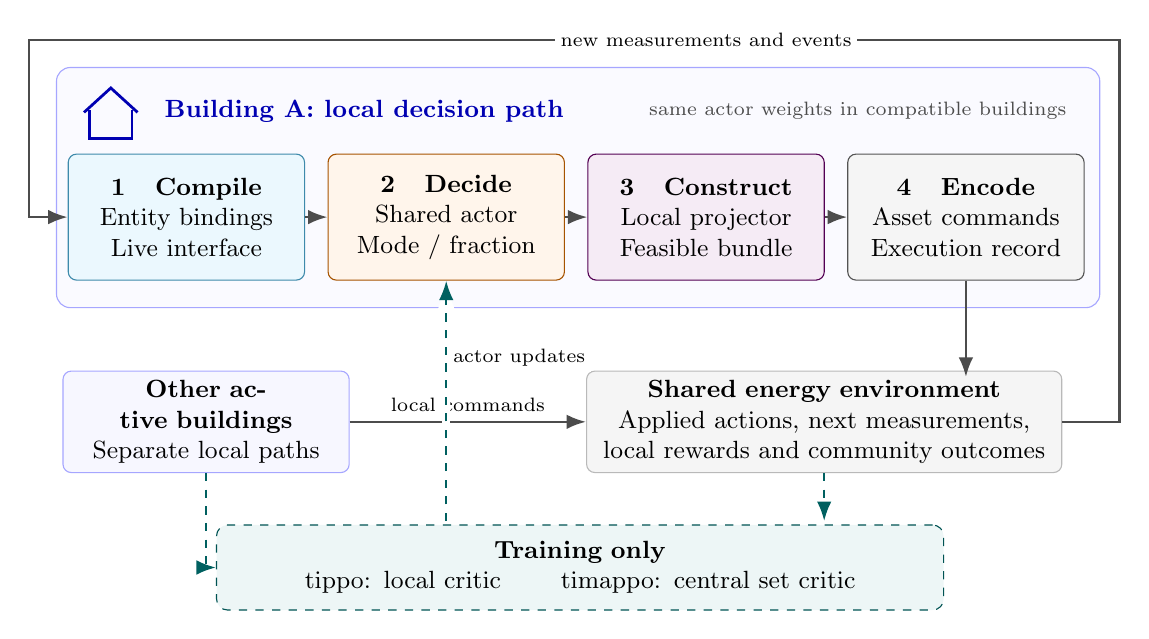
\begin{tikzpicture}[x=1cm,y=1cm,
  stage/.style={draw=#1!65!black,fill=#1!8,rounded corners=3pt,
    text width=2.65cm,minimum height=1.60cm,align=center,font=\small,inner sep=5pt},
  flow/.style={-Latex,line width=0.9pt,draw=black!70},
  train/.style={-Latex,dashed,line width=0.9pt,draw=teal!75!black}]
\draw[rounded corners=5pt,draw=blue!35,fill=blue!2] (-1.65,0.7) rectangle (11.6,-2.35);
% House icon marks a physical controller boundary.
\draw[blue!70!black,line width=1pt] (-1.30,0.13) -- (-.96,.44) -- (-.62,.13);
\draw[blue!70!black,line width=1pt] (-1.23,.16) -- (-1.23,-.2) -- (-.69,-.2) -- (-.69,.16);
\node[anchor=west,font=\small\bfseries,text=blue!70!black] at (-.4,.15) {Building A: local decision path};
\node[anchor=east,font=\scriptsize,text=black!70] at (11.3,.15) {same actor weights in compatible buildings};
\node[stage=cyan] (compile) at (0,-1.2) {\textbf{1\quad Compile}\\Entity bindings\\Live interface};
\node[stage=orange] (actor) at (3.3,-1.2) {\textbf{2\quad Decide}\\Shared actor\\Mode / fraction};
\node[stage=violet] (project) at (6.6,-1.2) {\textbf{3\quad Construct}\\Local projector\\Feasible bundle};
\node[stage=gray] (codec) at (9.9,-1.2) {\textbf{4\quad Encode}\\Asset commands\\Execution record};
\draw[flow] (compile) -- (actor);
\draw[flow] (actor) -- (project);
\draw[flow] (project) -- (codec);
\node[draw=blue!35,fill=blue!3,rounded corners=3pt,align=center,text width=3.4cm,minimum height=1.05cm,font=\small] (others) at (.25,-3.8) {\textbf{Other active buildings}\\Separate local paths};
\node[draw=gray!55,fill=gray!8,rounded corners=3pt,align=center,text width=5.8cm,minimum height=1.05cm,font=\small] (env) at (8.1,-3.8) {\textbf{Shared energy environment}\\Applied actions, next measurements,\\local rewards and community outcomes};
\draw[flow] (codec.south) -- (9.9,-3.23);
\draw[flow] (others.east) -- node[above,font=\scriptsize] {local commands} (env.west);
\draw[flow] (env.east) -- (11.85,-3.8) -- (11.85,1.05) -- (-2,1.05) -- (-2,-1.2) -- (compile.west);
\node[font=\scriptsize,fill=white,inner sep=2pt] at (6.6,1.05) {new measurements and events};
\node[draw=teal!65!black,fill=teal!7,dashed,rounded corners=4pt,text width=9cm,align=center,minimum height=1.08cm,font=\small] (critic) at (5.0,-5.65) {\textbf{Training only}\\\gls{tippo}: local critic \qquad \gls{timappo}: central set critic};
\draw[train] (env.south) -- (8.1,-5.06);
\draw[train] (others.south) -- (.25,-5.65) -- (critic.west);
\draw[train,preaction={draw=white,line width=3pt}] (3.3,-5.06) -- node[right,pos=.68,font=\scriptsize,fill=white,inner sep=2pt] {actor updates} (actor.south);
\end{tikzpicture}%
}

\caption{\gls{timarl} decision path within each building. Local construction precedes execution; the \gls{rec} critic participates only in training.}
\label{fig:timarl-architecture}
\end{figure}

Table~\ref{tab:timarl-components} identifies the role of each component. The same interface snapshot accompanies the decision through these stages, so a charger retains its identity when its observations become actor inputs and its selected power becomes an equipment command.

\begin{table}[htbp]
\centering
\caption{Main \gls{timarl} components and their interpretation in the running energy example.}
\label{tab:timarl-components}
\begin{tabularx}{\textwidth}{@{}p{0.22\textwidth}p{0.38\textwidth}X@{}}
\toprule
\textbf{Component} & \textbf{Generic role} & \textbf{Energy example} \\
\midrule
\gls{tic} & Binds deployment-neutral member contracts to current entities, observations, events, health, groups, bounds, and constraints & Adds a known charger group when it becomes active; scopes failure to the affected group; contracts \gls{v2g} when its evidence is stale \\
Hierarchical typed encoder & Aggregates observations by channel and sensor before forming a local latent state & Keeps two charger sessions distinct through semantic and structural identities without learning an embedding for a concrete charger identifier \\
Shared hybrid actor & Produces one categorical mode and one bounded continuous fraction for each active group & Controls two chargers, one battery, and one deferrable service with shared group-type heads rather than an asset-specific output head \\
Analytic local projector & Applies validity, dynamic bounds, service floors, and joint total/per-phase headroom & Preserves an urgent \gls{ev} or mandatory deferrable start while scaling competing charging decisions to the available connection capacity \\
Local or central set critic & Supplies \gls{tippo} local values or \gls{timappo} values conditioned on the active member set & Retains the same decentralised actor while comparing independent and \gls{rec}-aware value estimation \\
\bottomrule
\end{tabularx}
\end{table}

The architecture is deliberately asymmetric between training and operation. The actor remains local in both phases. Centralisation is introduced only in \gls{timappo}'s value function and the experiment infrastructure, where it can improve credit assignment without creating a runtime dependency on unrestricted global state. \gls{rec} observations remain typed observation parts with explicit scope, provenance, time, and health.

\section{Typed Interfaces and Runtime Compilation}
\label{sec:runtime-interface-model}

The interface provides a stable vocabulary for a changing installation. A schema declares what a resource means and which capabilities it can expose; compilation binds that declaration to the resources and evidence present at the current step. This separates a new instance of a familiar charger from a new kind of equipment requiring additional control semantics.

\subsection{Schemas, Entities, and Dynamic Module Instances}
\label{sec:timarl-entities}

A capability schema describes the potential interface of an agent. It identifies the agent role, module types, observation templates, action-group templates, constraints, compatibility requirements, and fallback semantics. Runtime state identifies which module instances and controlled entities are active now. Separating the two prevents fast-changing values such as \gls{soc} or connection state from being treated as schema revisions.

A building can contain several instances of the same module type. In the running example, agent $A$ contains two charger instances, one stationary battery, one deferrable-service module, and one main meter:

\begin{equation}
\mathcal{M}_{A,t}
=
\{m^{\mathrm{meter}}_1,
  m^{\mathrm{charger}}_1,
  m^{\mathrm{charger}}_2,
  m^{\mathrm{battery}}_1,
  m^{\mathrm{def}}_1\}.
\label{eq:running-modules}
\end{equation}

Here $\mathcal M_{A,t}$ is the module set of building $A$ at time $t$; the superscripts identify module types and the subscripts distinguish their instances. Each charger can be related to a currently connected \gls{ev} session. The following observation identifies the \gls{soc} source for one such session:

\begin{quote}\small
\begin{minipage}{\linewidth}
\texttt{semantic type: EV\_SOC}\\
\texttt{entity: ev\_session\_17}\\
\texttt{source module: charger\_1}
\end{minipage}
\end{quote}

The source and session identities distinguish this measurement from the \gls{soc} of the vehicle connected to \texttt{charger\_2}. The corresponding action group is similarly bound:

\begin{quote}\small
\begin{minipage}{\linewidth}
\texttt{group type: EV\_CHARGER\_MODE}\\
\texttt{owner module: charger\_1}\\
\texttt{target entity: ev\_session\_17}
\end{minipage}
\end{quote}

The compiler represents these relationships as typed edges such as \texttt{owns}, \texttt{connected\_to}, \texttt{observes}, \texttt{controls}, and \texttt{requires}. Entity binding is encoded in the interface semantics and does not depend on position in a flat vector.

When \texttt{charger\_3} is installed, a module-addition event creates a new module node, its observation parts, one \gls{ev}-charger action-group instance, valid port instances, and the relevant constraint edges. The neural network is not extended with a new permanent head. The same group and port decoder used for the existing chargers is applied to the new instance. Removing the charger removes that subgraph. A semantically unknown module is admitted only when a compatible parent type and decoder are available; otherwise its learned control path remains inactive and fallback semantics apply.

The implementation deliberately separates four identifiers that flat action layouts often conflate. A member owns the local controller boundary; a charger identifies installed infrastructure; an \gls{ev} identifies a vehicle; and a session records the temporary occupancy of one charger by one \gls{ev}. A domestic charger can retain the same vehicle over many sessions, whereas one office charger can serve several vehicles in one day. The action group belongs to the physical charger, while service observations belong to the currently bound session. Session replacement therefore rebinds runtime values without rebuilding an unchanged charger structure.

\subsection{Typed Observation Parts and Community Context}
\label{sec:timarl-observations}

An observation part is a typed object with an identity and declared semantics. A representative definition is

\begin{equation}
o_k
=
\left(
\tau_k,
\mathrm{id}_k,
\mathrm{entity}_k,
\mathrm{source}_k,
 x_k,
 u_k,
 q_k,
 h_k,
 t_k,
 s_k
\right),
\label{eq:observation-part}
\end{equation}

where $k$ indexes an observation part, $\mathrm{id}_k$ identifies that part, $\mathrm{entity}_k$ identifies the entity described, and $\mathrm{source}_k$ identifies its source. The remaining entries are $\tau_k$, the semantic type, $x_k$ the value, $u_k$ the unit, $q_k$ quality or uncertainty metadata, $h_k$ the health state, $t_k$ the timestamp, and $s_k$ the scope. The scope can be self, local, neighbourhood, \gls{rec}, or global. The source can be a physical sensor, derived signal, forecast, external platform, or coordinator message.

\gls{rec} information is represented through the same object model. A building may receive numerical aggregates such as \gls{rec} net demand, transformer loading, remaining headroom, \gls{pv} surplus, a price multiplier, or a demand-response target. These values do not reveal the raw private state of another building. Their provenance and health remain explicit:

\begin{quote}\small
\begin{minipage}{\linewidth}
\texttt{semantic type: COMMUNITY\_TRANSFORMER\_LOADING}\\
\texttt{scope: community; source: platform\_service}\\
\texttt{unit: percent; health: HEALTHY}
\end{minipage}
\end{quote}

In the energy instantiation, an \gls{ev} connected from 08:00 until 18:00 with a current \gls{soc}, target \gls{soc}, maximum charging power, and departure requirement already exposes the information from which a policy can learn temporal flexibility. Useful derived quantities such as time to departure, remaining required energy, or required average charging power can be supplied as typed observation parts when they improve learning or interpretability. Their inclusion is fixed by the experimental configuration.

\Cref{tab:timarl-running-observations} lists representative observation parts for the running example.

\begin{table}[htbp]
\centering
\small
\caption{Representative typed observation parts for a building with two chargers. Values are illustrative.}
\label{tab:timarl-running-observations}
\begin{tabularx}{\textwidth}{@{}p{0.19\textwidth}p{0.16\textwidth}p{0.13\textwidth}p{0.12\textwidth}X@{}}
\toprule
\textbf{Semantic type} & \textbf{Entity/source} & \textbf{Value} & \textbf{Scope} & \textbf{Decision meaning} \\
\midrule
House net power & main meter & 2.1 kW & self & Current aggregate import used to evaluate local electrical limits \\
\gls{ev} \gls{soc} & session 17 / charger 1 & 0.35 & local & Energy state of the \gls{ev} controlled through charger 1 \\
\gls{ev} target \gls{soc} & session 17 & 0.80 & local & Minimum service target at departure \\
Departure time & session 17 & 10 h & local & Temporal slack available to the charging policy \\
\gls{ev} \gls{soc} & session 28 / charger 2 & 0.62 & local & Distinct \gls{soc} bound to charger 2 and its connected session \\
Battery \gls{soc} & battery 1 & 0.70 & local & Available storage state \\
\gls{rec} headroom & platform service & 5.5 kW & \gls{rec} & Aggregate remaining shared capacity made visible to all authorised agents \\
\gls{rec} peak state & platform service & high & \gls{rec} & \gls{rec} context used by local actors and the reward \\
\bottomrule
\end{tabularx}
\end{table}

\subsection{Dynamic Action Groups and Typed Parameterised Ports}
\label{sec:timarl-action-ports}

The output interface is organised around action-group instances. Each controllable module creates one or more groups whose ports are mutually exclusive within the group but can be combined with ports from other groups. For example,

\begin{align}
\mathcal{P}_{\mathrm{charger}_1,t}
&=\{\textsc{idle-ev},\textsc{charge-ev}(p),\textsc{discharge-ev}(p)\},\\
\mathcal{P}_{\mathrm{battery}_1,t}
&=\{\textsc{idle-battery},\textsc{charge-battery}(p),\textsc{discharge-battery}(p)\},\\
\mathcal{P}_{\mathrm{def}_1,t}
&=\{\textsc{idle},\textsc{start}\}.
\end{align}

Each set $\mathcal P$ lists the ports of the named resource at time $t$. In these examples, the argument $p$ denotes a requested physical power; the deferrable service has a discrete start decision. An action port itself is a typed callable capability:

\begin{equation}
p
=
\left(
\tau_p,
\mathrm{id}_p,
\mathrm{group}_p,
\mathrm{owner}_p,
\Theta_p,
U_p,
B_{p,t},
V_{p,t},
D_p,
K_p
\right),
\label{eq:action-port}
\end{equation}

where $\tau_p$ is the port type, $\mathrm{id}_p$ its identity, $\mathrm{group}_p$ the action group to which it belongs, and $\mathrm{owner}_p$ its owning module. The remaining entries are $\Theta_p$, the parameter schema, $U_p$ the units, $B_{p,t}$ the current parameter domain, $V_{p,t}$ the validity state, $D_p$ the observation and capability dependencies, and $K_p$ the resource effects used by local constraints, critics, and optional safety checks.

A new charger creates another instance of the charger action group. It does not create another set of network parameters. The implemented actor emits a categorical mode and a Beta-distributed fraction in $[0,1]$ for every active group. The fraction is relative to the currently compiled physical upper bound and is converted to a signed simulator command only once by the codec. This convention avoids applying a health-dependent or topology-dependent bound twice. A deferrable start is indivisible: after \textsc{start} is selected, its typed cycle profile determines the subsequent demand rather than a continuous power fraction.

\begin{table}[htbp]
\centering
\small
\caption{Representative action ports for two charger instances and one stationary battery.}
\label{tab:timarl-running-ports}
\begin{tabularx}{\textwidth}{@{}p{0.17\textwidth}p{0.17\textwidth}p{0.16\textwidth}p{0.22\textwidth}X@{}}
\toprule
\textbf{Port} & \textbf{Owner/target} & \textbf{Parameter} & \textbf{Current validity and bounds} & \textbf{Dependencies and local effects} \\
\midrule
Charge \gls{ev} & charger 1 / session 17 & power [kW] & valid, $[0,7.2]$ & connected session; increases house import \\
Discharge \gls{ev} & charger 1 / session 17 & power [kW] & valid, $[0,4.0]$ & \gls{v2g}, trustworthy \gls{soc}, reserve; reduces house import \\
Charge \gls{ev} & charger 2 / session 28 & power [kW] & valid, $[0,11.0]$ & distinct connection and \gls{ev} state; increases house import \\
Discharge \gls{ev} & charger 2 / session 28 & power [kW] & absent & charger 2 has no \gls{v2g} capability \\
Discharge battery & battery 1 & power [kW] & valid, $[0,3.0]$ & battery \gls{soc} and reserve; reduces house import \\
\bottomrule
\end{tabularx}
\end{table}

For example, suppose \texttt{charger\_1} is rated at 7.4~kW but the current connection and \gls{ev} state reduce its compiled charging bound to 4.0~kW. A sampled fraction of 0.75 requests 3.0~kW. The network output remains in the same numerical domain when the available bound later changes; the interface gives the output its current physical meaning. The trace stores the selected mode, fraction, compiled bound, requested command, projected command, and applied simulator value separately.

\section{Policy Architecture and Multi-Agent Learning}
\label{sec:tip-and-learning}
\label{sec:timarl-multiagent-learning}

Once the interface has been compiled, the actor must interpret its current observations and produce a decision for each controllable group. Shared processing allows another known charger to reuse the existing policy. Centralised training can then account for the interaction between buildings while preserving the local information available during operation.

\subsection{Local Information and Hierarchical Encoding}
\label{sec:timarl-local-info}

Each agent executes a logically local \gls{tip}. A building actor receives its compiled interface, optional memory, and authorised aggregate \gls{rec} observations. It does not receive the raw loads, \gls{ev} states, or private service requirements of other buildings. This boundary is identical during evaluation and deployment; privileged information used by a central critic during training is not silently passed to the actor.

The current implementation shares one actor across all compatible members:

\begin{equation}
\pi_i
=
\pi_{\theta}
\left(
\mathcal{I}_{i,t},m_{i,t}
\right),
\label{eq:role-sharing}
\end{equation}

Here $\pi_i$ is the policy instance of agent $i$, $\pi_\theta$ is the shared actor with parameters $\theta$, $\mathcal I_{i,t}$ is its local snapshot, and $m_{i,t}$ is optional local memory. Parameter sharing preserves separate observations. House $A$ and House $B$ execute the same weights on different local snapshots, and member role remains an encoded feature. The compiler rejects unknown semantic or action-group types rather than silently allocating a random representation. This keeps zero-shot admission limited to new instances and compositions of known contracts.

This structure supports population changes without a permanent actor slot per agent. A new building instantiates the appropriate local policy family after schema compatibility has been checked. Removing a building removes its actor instance from the active population; the shared parameter set and the actors of the remaining agents are unchanged.

\label{sec:timarl-local-encoder}

The compiled local interface is encoded as variable-cardinality typed sets. The hierarchy follows the simulator's measurement structure: observation parts are grouped into channels, channels into sensors, and sensors into the local member representation. Structural relations remain available when an action group asks for its relevant observations. This hierarchy follows the implemented measurement structure and preserves the binding needed by the decoder.

Each observation token combines its normalised value with quality and validity indicators, health, semantic type, sensor type, channel type, unit, scope, declared use, a deterministic semantic fingerprint, and temporal-horizon features. The first mapping is

\begin{align}
z^{o}_{k}
&=
E^{o}_{\theta}
\left(
x_k,q_k,h_k,e_{\tau_k},e_{\mathrm{sensor}},e_{\mathrm{channel}},
e_{u_k},e_{s_k},e_{\mathrm{use}},f^{\mathrm{id}}_k,f^{\mathrm{time}}_k
\right).
\end{align}

Here $z^o_k$ is the embedding of observation part $k$, and $E^o_\theta$ is its learned encoder. The values $x_k$, $q_k$, and $h_k$ retain the meanings in Equation~\ref{eq:observation-part}; each $e$ is an embedding of the named metadata field. The features $f^{\mathrm{id}}_k$ and $f^{\mathrm{time}}_k$ encode semantic identity and temporal information. Permutation-equivariant relational layers aggregate observation tokens within their channels and sensors, followed by learned pooling over the local sensor set:

\begin{equation}
z_{i,t}
=
F_{\theta}
\left(
\left\{\left\{\{z^o_k\}_{k\in c}\right\}_{c\in s}\right\}_{s\in i}
\right).
\label{eq:tip-encoder}
\end{equation}

The mapping $F_\theta$ aggregates the nested sets: $k$ indexes observation parts, $c$ channels, and $s$ sensors belonging to member $i$. The common latent $z_{i,t}$ summarises the complete local decision context. Concrete asset identifiers are not learned as permanent embeddings. Instance distinction is carried by the compiled structural binding and deterministic observation identity, while semantic families determine reusable parameters. Reordering observations, chargers, or members therefore does not change the intended meaning.

Each active action group starts from its type embedding and the local latent. In the action-conditioned variant, the group also queries observation tokens related to its owner, target entity, and dependencies. The two chargers can use the same mode and fraction heads while attending to different sessions. Attention across the active group set then exposes local competition before decoding. Adding a charger adds one group evaluation; it does not change the actor or critic parameter count.

During replay and \gls{bc} updates, immutable type indices and set membership are prepared once and reused across optimisation epochs. Runtime values and health are never cached as static input. Packed evaluation removes repeated per-agent device transfers while preserving the same set semantics. These changes affect throughput, not the mathematical information surface.

\subsection{Dynamic Grouped Action Decoding}
\label{sec:timarl-action-decoder}

The actor does not contain a permanent neural head for each asset instance. A group-type head is applied to every active group of that type. For group $g$ and candidate mode $m$,

\begin{equation}
\ell_{i,g,m,t}
=
f^{\mathrm{select}}_{\theta}
\left(
 z_{i,t},z_{i,g,t},e_{\tau_g}
\right),
\label{eq:port-logit}
\end{equation}

Here $\ell_{i,g,m,t}$ is the logit for candidate mode $m$ of group $g$, $z_{i,g,t}$ is its contextual embedding, $e_{\tau_g}$ represents its type, and $f^{\mathrm{select}}_\theta$ is the shared selection head. The categorical mode is selected after invalid modes have been masked:

\begin{equation}
\Pr
\left(
 m_{i,g,t}=m
\right)
=
\operatorname{Softmax}_{m\in\mathcal{M}^{\mathrm{valid}}_{i,g,t}}
\left(
\ell_{i,g,m,t}
\right).
\label{eq:port-selection}
\end{equation}

Here $m_{i,g,t}$ is the selected mode, $\mathcal M^{\mathrm{valid}}_{i,g,t}$ is its admissible candidate set, and Softmax normalises the corresponding logits into probabilities. A second head generates positive Beta parameters. Sampling $u_{i,g,t}\sim\operatorname{Beta}(\alpha_{i,g,t},\beta_{i,g,t})$ gives the bounded fraction

\begin{equation}
\eta_{i,g,t}
=
u_{i,g,t},
\qquad
(\alpha_{i,g,t},\beta_{i,g,t})
=
d_{\tau_g}(z_{i,g,t}).
\label{eq:port-parameters}
\end{equation}

The decoder $d_{\tau_g}$ produces positive shape parameters $\alpha_{i,g,t}$ and $\beta_{i,g,t}$ for the Beta distribution; its sample $u_{i,g,t}$ supplies the fraction $\eta_{i,g,t}$. The log probability used by \gls{ppo} is the sum of the categorical and Beta terms. At training time the two parts are sampled. Deterministic replay can use categorical argmax or an \texttt{expected\_signed} rule that combines charge and discharge probabilities, the Beta mean, a configurable gain, a deadband, and a non-idle logit margin. These controls were added because an apparently small stochastic preference can become an implausibly persistent deterministic charge or discharge command after export.

All groups are decoded as one bundle from the same local context. A representative raw bundle is

\begin{equation}
a^{\mathrm{raw}}_{A,t}
=
\left\{
\begin{array}{l}
\texttt{charger\_1}:\textsc{charge-ev}(4.0\ \mathrm{kW}),\\
\texttt{charger\_2}:\textsc{charge-ev}(3.5\ \mathrm{kW}),\\
\texttt{battery\_1}:\textsc{discharge-battery}(1.0\ \mathrm{kW}),\\
\texttt{deferrable\_1}:\textsc{start}
\end{array}
\right\}.
\label{eq:running-raw-bundle}
\end{equation}

Here $a^{\mathrm{raw}}_{A,t}$ collects the four proposed decisions for building $A$ at time $t$; their powers are illustrative. The bundle-level representation allows the actor to learn priorities among the two \gls{ev} sessions, battery use, a pending service, and \gls{rec} conditions. It does not by itself guarantee that the combined power remains within local electrical limits or that an urgent service remains feasible. Those requirements are handled by the final local construction.

\subsection{Centralised Training and Local Execution}
\label{sec:timarl-joint-training}

\gls{timarl} does not require a \gls{rec} controller agent. Each building acts independently from its own compiled interface and authorised \gls{rec} observations. The method becomes multi-agent because the local bundles form one joint action, the physical transition depends on that joint action, local actions compete for shared resources, and rewards include local and \gls{rec} consequences.

At each training step, the constructed local bundles form the joint action in Equation~\ref{eq:joint-action}. Its transition produces the next interfaces, local rewards, and \gls{rec} outcomes. Simultaneous charging can reduce shared headroom even when both buildings satisfy their own connection limits. Repeated interaction supplies the experience from which local actors learn those collective consequences.

Joint training means that actor updates are derived from the same joint transition. It does not mean that actors share private runtime inputs or that one global actor replaces them. Stable member identities govern the rollout when population changes. A joining member has no predecessor in Generalised Advantage Estimation; a departing member receives a terminal boundary; members that remain can bootstrap across the topology event. The rollout is not cleared and the networks are not resized.

\label{sec:timarl-central-critic}

A conventional central critic often concatenates all agent observations. That representation is tied to a fixed order and population. \gls{tippo} avoids centralisation and estimates $V_i$ from the local typed snapshot. \gls{timappo} retains the same actor but estimates values from the variable active set.

The implemented central critic encodes each member with the same typed snapshot encoder, mean-pools the active local latents into a \gls{rec} summary, and evaluates each stable member identity from its local and \gls{rec} representations:

\begin{equation}
V_{\phi,i,t}
=
g_{\phi}
\left(
z_{i,t},
\frac{1}{|\mathcal{N}_t|}
\sum_{j\in\mathcal{N}_t}z_{j,t}
\right).
\label{eq:graph-critic}
\end{equation}

Here $V_{\phi,i,t}$ is the value estimate for member $i$, $g_\phi$ is the learned value mapping, and $z_{j,t}$ is the encoded snapshot of active member $j$. The mean contains all $|\mathcal N_t|$ active members. The mapping is permutation equivariant: reordering members reorders their values but does not alter their association. Cardinality can change without reconstructing a joint input layer. Mean pooling supplies a compact \gls{rec} context. Distinct feeder neighbourhoods with identical aggregate summaries receive the same pooled representation. Representing those neighbourhoods explicitly would require a richer critic input or aggregation rule.

\subsection{Proximal Policy Optimisation with Typed Interfaces}
\label{sec:timarl-backbones}

\gls{timarl} defines the interface, actor structure, local bundle semantics, and population handling. The current learner supports two controlled \gls{ppo} variants.

\paragraph{TI-PPO.}
The shared actor and a parameter-shared local critic are updated from local member trajectories. This is the typed one-agent learner applied independently across the active population. It isolates the effect of the interface and actor from centralised value estimation.

\paragraph{TI-MAPPO.}
The actor is paired with the central set critic in \cref{eq:graph-critic}. The critic may use the active joint training context; the actor retains its local information boundary. A checkpoint pins the backbone and critic kind, so a \gls{tippo} state cannot be loaded into \gls{timappo} by accident.

For a transition generated by old parameters $\theta_{\mathrm{old}}$, the hybrid group probability ratio is

\begin{equation}
r_{i,g,t}(\theta)
=
\exp\left[
\log\pi_{\theta}(m_{i,g,t},\eta_{i,g,t}\mid\mathcal{I}_{i,t})
-
\log\pi_{\theta_{\mathrm{old}}}(m_{i,g,t},\eta_{i,g,t}\mid\mathcal{I}_{i,t})
\right].
\label{eq:timarl-ratio}
\end{equation}

Here $r_{i,g,t}(\theta)$ compares the current and collection-policy probabilities for the same recorded mode, fraction, and interface. The parameters $\theta_{\mathrm{old}}$ identify the collection policy. With joint-agent credit, the clipped \gls{ppo} objective uses the sum of group log probabilities for that member. With typed-group credit, the ratio and advantage remain attached to group $g$:

\begin{equation}
L^{\mathrm{group}}(\theta)
=
\mathbb{E}_{i,g,t}
\left[
\min\left(
r_{i,g,t}(\theta)\hat{A}_{i,g,t},
\operatorname{clip}(r_{i,g,t}(\theta),1-\epsilon,1+\epsilon)
\hat{A}_{i,g,t}
\right)
\right].
\label{eq:timarl-group-ppo}
\end{equation}

Here $\hat A_{i,g,t}$ is the advantage estimate assigned to group $g$, $\epsilon$ is the clipping tolerance, and the expectation averages recorded agent--group transitions. The operator $\operatorname{clip}$ bounds the ratio to $[1-\epsilon,1+\epsilon]$. The group critic supplies a matching baseline. \gls{ev} service and charger-constraint consequences are routed to the responsible charger family; stationary-storage consequences reach the storage group; deferrable completion reaches its start group. Economic settlement and genuinely shared grid effects remain common. This avoids teaching the second charger that it caused a service failure belonging to the first, while preserving \gls{rec} coupling.

The comparison with \gls{matd3} in Chapter~\ref{chap:control-benchmark} retains a practical reference from a different learning family. Attribution to the interface is assessed more directly through \gls{ppo}-based controls with matched actor inputs, training budgets, and protection.

\subsection{Training Data and Time Resolution}
\label{sec:timarl-learning-engineering}

Moving the controller to 15-minute data increased the effective learning horizon and exposed numerical failures that were less visible in the earlier hourly experiments. \gls{timarl} therefore treats the physical duration of a transition as part of the learner contract. When $\gamma_{\mathrm{ref}}$ and $\lambda_{\mathrm{ref}}$ are declared for reference duration $\Delta t_{\mathrm{ref}}$, the factors used at runtime are

\begin{equation}
\gamma_{\Delta t}=\gamma_{\mathrm{ref}}^{\Delta t/\Delta t_{\mathrm{ref}}},
\qquad
\lambda_{\Delta t}=\lambda_{\mathrm{ref}}^{\Delta t/\Delta t_{\mathrm{ref}}}.
\label{eq:timarl-timebase}
\end{equation}

Here $\Delta t$ is the transition duration and $\Delta t_{\mathrm{ref}}$ the reference duration. The factors $\gamma$ and $\lambda$ control reward discounting and Generalised Advantage Estimation respectively, preserving their declared time basis as the step changes. The implementation normalises critic targets, uses a Huber value loss by default, clips policy ratios and gradient norms, and records approximate \gls{kl} divergence, clipping fraction, explained variance, and finite-gradient checks. Advantages can be normalised globally or per stable member identity. Entropy coefficients can differ by action-group family; a charger and a deferrable start do not need the same exploration pressure. A policy anchor can constrain movement from a selected actor and can be reset deliberately when a checkpoint is resumed.

The rollout is on-policy and retains the raw typed decision, projected decision, intervention scope, stable agent and group identities, reward decomposition, termination semantics, current and next snapshot hashes, and simulator execution feedback. Teacher actions and auxiliary-planning examples never enter that \gls{ppo} rollout. This boundary matters: an update remains attributable to experience generated by the current policy even when demonstrations are used elsewhere in training.

\label{sec:timarl-prior-knowledge}

The use of prior knowledge in Section~\ref{sec:control-ablations} motivates an optional \gls{bc} warm start with \gls{rbc} Smart Local (the implementation class \texttt{RBCSmartPolicy}). The teacher acts on the physical simulator interface; its requested commands are decoded back into the active typed groups and stored with the exact interface snapshot on which they were valid. Pretraining updates the actor only. The critic is not trained from teacher returns, and the complete demonstration snapshots are discarded after pretraining.

Idle actions dominate many annual trajectories. A plain average cross-entropy loss can therefore learn an impressive cloning accuracy while missing the charge, discharge, \gls{v2g}, or start events that make the teacher useful. The implementation supports bounded inverse-frequency weighting and a hierarchical mode mean. It can run a final unweighted calibration phase so that balancing rare actions does not permanently distort the deployed prior.

Two optional causal auxiliaries were added after the warm-start experiments exposed sparse service decisions. The \gls{ev} planner labels typed states using only current service variables and declared forecasts: urgent charging, price-aware delay, authorised \gls{v2g} with departure reserve, or idle. The storage planner identifies \gls{pv} capture, low-price charging, high-price discharge, and idle from the same deployment-visible surface. Each auxiliary predicts both mode and fraction, trains the actor only, and keeps a bounded reservoir stratified by decision reason. Rare urgent or arbitrage examples therefore survive without contaminating the \gls{ppo} rollout.

These planners supply training labels; runtime decisions remain with the actor and analytic projector. Pure \gls{timappo}, \gls{bc} warm start, \gls{ev} auxiliary, storage auxiliary, and their combinations remain separate ablations. This separation makes the contribution of prior knowledge testable: prior knowledge is attached to a typed and causal state, while the learned actor still owns execution.

\section{Constraint Handling and Degraded Operation}
\label{sec:tcg-safety}

The compiled interface serves two connected purposes in protection. It determines which decisions remain meaningful under the current evidence, then supplies the physical and service constraints used to construct their joint local effect. A charger fault and a building power limit therefore enter different stages of the same decision path.

\subsection{Health-Aware Causal Compilation}
\label{sec:timarl-health}

Health is part of the interface semantics and is also available to the neural network. The implemented states are \textsc{healthy}, \textsc{degraded}, \textsc{stale}, \textsc{missing}, \textsc{failed}, and \textsc{unknown}. Fault evidence remains a separate record. A simulator event such as \texttt{dropout} or \texttt{stuck} is not mapped to one universal health label; the compiler considers event duration, freshness, criticality, declared availability, channel semantics, and recovery hysteresis.

A charger failure disables only the associated charger group and its ports. Other modules controlled by the member remain active. A stale \gls{ev} \gls{soc} can preserve charging while blocking \gls{v2g} because the discharge reserve can no longer be established. Failure of the main house meter has a wider consequence: the complete member is isolated when aggregate import or phase headroom cannot be verified. Loss of a \gls{rec} signal removes that coordination input but leaves the local controller available. During a grid outage, charging, \gls{v2g}, and a new deferrable start are blocked; safe stationary-storage discharge may remain available when its local dependencies still hold.

The compiler computes the transitive effect of a health event through a dependency closure:

\begin{equation}
\mathcal{H}^{\star}_{i,t}
=
\operatorname{Closure}
\left(
\mathcal{H}_{i,t},D_{i,t}
\right),
\label{eq:health-closure}
\end{equation}

where $D_{i,t}$ is the declared dependency relation, $\operatorname{Closure}$ propagates the observed health state $\mathcal H_{i,t}$ through it, and $\mathcal H^\star_{i,t}$ records the resulting consequences. These consequences concern observations, ports, groups, bounds, local constraints, and operational modes. For the \gls{ev} \gls{soc} example, the closure can be summarised as

\begin{equation}
\mathcal P^{\mathrm{valid}}_{i,t}
\leftarrow
\mathcal P^{\mathrm{valid}}_{i,t}\setminus
\{p:\tau_p=\textsc{discharge-ev},\ \mathrm{owner}_p=\texttt{charger\_1}\}.
\label{eq:timarl-health-port-removal}
\end{equation}
Here $\mathcal P^{\mathrm{valid}}_{i,t}$ is the valid port set of member $i$, $\tau_p$ is a port's type, and $\mathrm{owner}_p$ identifies its equipment. Set subtraction removes only the discharge capability of the affected charger. Charging remains available only if its own dependencies and service constraints can still be established.

The dependency rule changes the decision interface itself, giving the policy an explicit account of the capabilities still available. Recovery is explicit: a group or port returns only after its declared fresh-data and hysteresis conditions hold. The closure log records the subject, state, rule, consequence, and duration used in that decision.

The compiler rebuilds structural plans only when topology changes. Values, health evidence, session identity, validity, and bounds are refreshed at every step without treating routine runtime churn as a new neural architecture. This separation is important in the 15-second stress case, where value and session updates occur far more frequently than asset installation or removal.

\subsection{Constraint-Aware Local Bundle Construction}
\label{sec:timarl-local-feasibility}

Local hard constraints should not depend exclusively on a negative reward. An actor can learn to reduce violations, but safety-critical electrical and service limits require explicit semantics. \gls{timarl} keeps the learned preference in the raw bundle and applies a constraint-aware parameterisation to obtain the final local bundle.

Let $a^{\mathrm{raw}}_{i,t}$ denote the decoded bundle and $\mathcal{A}^{\mathrm{loc}}_{i,t}$ the feasible set induced by the local typed graph. The construction is

\begin{equation}
\bar{a}_{i,t}
=
\Phi_i
\left(
 a^{\mathrm{raw}}_{i,t},
 \mathcal{A}^{\mathrm{loc}}_{i,t}
\right),
\qquad
\bar{a}_{i,t}\in\mathcal{A}^{\mathrm{loc}}_{i,t}.
\label{eq:local-bundle-construction}
\end{equation}

Here $\Phi_i$ constructs the final bundle $\bar a_{i,t}$ from the raw decisions and the current local feasible set. The implementation uses an analytic joint projector. It first rejects a removed or invalid group, applies a forced typed fallback when one exists, clips the learned fraction to $[0,1]$, and respects the minimum operating power declared by the selected port. It then reserves mandatory deferrable starts and the \gls{ev} charging power needed to remain within the configured service schedule. Remaining charge and discharge requests are jointly scaled against total and phase-specific import or export headroom. A command that falls below its typed operating floor after scaling returns to \textsc{idle}.

For the running example, one local constraint is

\begin{equation}
P^{\mathrm{ch1}}_t
+
P^{\mathrm{ch2}}_t
+
P^{\mathrm{def}}_t
-
P^{\mathrm{bess,dis}}_t
\leq
P^{\max}_{A,t}.
\label{eq:running-local-constraint}
\end{equation}

Here $P^{\mathrm{ch1}}_t$ and $P^{\mathrm{ch2}}_t$ are the two charging powers, $P^{\mathrm{def}}_t$ is the deferrable load, and $P^{\mathrm{bess,dis}}_t$ is stationary-battery discharge. The quantity $P^{\max}_{A,t}$ is the remaining import headroom after accounting for the other loads and generation of building $A$. This total limit is evaluated together with phase incidence. If both chargers lie on L1, unused headroom on L3 cannot make their combination feasible. A three-phase service contributes to all three phase rows according to its declared incidence. The projector can retain a configurable headroom reserve and a completion margin for deferrables. This construction resolves competition within the member; \gls{rec} coordination remains with the learned policies.

Two diagnostics distinguish a useful feasibility mechanism from one that hides poor policy learning:

\begin{align}
I^{\mathrm{loc}}_t
&=\mathbb{1}\left[a^{\mathrm{raw}}_{i,t}\notin\mathcal{A}^{\mathrm{loc}}_{i,t}\right],\\
D^{\mathrm{loc}}_t
&=\left\|\bar{a}_{i,t}-a^{\mathrm{raw}}_{i,t}\right\|.
\end{align}

Here $I^{\mathrm{loc}}_t$ uses the indicator $\mathbb 1$ to record an infeasible raw bundle, and $D^{\mathrm{loc}}_t$ measures its adjustment. The norm is evaluated on the common physical-command vector after decoding; discrete mode changes are counted separately. Frequent or large adjustments indicate reliance on the projector and weak learning of coherent bundles. Requested, projected, and applied actions remain separate in the transition record, so a physically safe trajectory cannot conceal an infeasible raw policy. The optional shield-aware update removes an intervened group from the \gls{ppo} policy loss and can distil the final feasible decision into that group; unrelated groups remain eligible for learning.

\subsection{Shared Limits and Operational Supervision}
\label{sec:timarl-tcg}
\label{sec:timarl-shared-monitor}
\label{sec:timarl-runtime-assurance}

The \gls{tcg} records ownership, connection, dependency, and constraint relations. A charger contributes power to its building and to the phases on which it operates. These relations supply local construction and identify the shared resources affected by the resulting commands. The central set critic uses member summaries; the \gls{tcg} is the physical description supporting the decision process.

For buildings sharing a transformer, the \gls{rec} limit can be written as
\begin{equation}
\sum_{i\in\mathcal N_t}K_i^{\mathrm{import}}(\bar a_{i,t})
\leq P^{\max}_{\mathrm{transformer},t}.
\label{eq:running-shared-constraint}
\end{equation}
Here $K_i^{\mathrm{import}}$ maps member $i$'s constructed action to its resulting import under the current physical state, and $P^{\max}_{\mathrm{transformer},t}$ is the permitted aggregate import. The sum spans the active members $\mathcal N_t$. Satisfaction of each building's local limit alone does not establish this shared inequality. In the current method, \gls{rec} observations, coupled rewards, and centralised value estimation support learned coordination; residual shared violations remain part of the evaluation.

Operational supervision sits outside this learned coordination. The Fail-Safe Supervisor described in Chapter~\ref{chap:energAIze} validates equipment requests, limits them when necessary, and supplies a rapid rule-based fallback when inference is unavailable. Within \gls{timarl}, dependency closure can already disable an affected group or isolate a member whose essential measurements are missing. The execution record distinguishes those interface decisions, local projection, supervisory intervention, and the final equipment response. Later retraining can therefore retain the circumstances of an intervention without attributing the fallback's outcome to an action the actor never executed.

This division preserves a precise scope of authority. The local construction enforces the encoded member constraints when the feasible set is non-empty, the physical model is correct, and the procedure terminates normally. An infeasible service obligation is recorded as unmet; electrical protection cannot create missing capacity or charging time. \gls{rec}-wide hard enforcement would require a declared allocation or jointly certified constraint mechanism in addition to the local projector.

\section{Compatibility and Deployment}
\label{sec:timarl-compatibility-explainability}

\subsection{Interface Snapshots and Admission}
\label{sec:timarl-compatibility}

Every decision is associated with an immutable interface snapshot containing active entities, observation parts, action groups, ports, validity, bounds, dependencies, health, and schema versions. The snapshot allows an experiment transition to be reconstructed even when the runtime topology subsequently changes.

Before a checkpoint is restored, its compatibility signature is checked against the current contract, schema, type registry, health rules, learning backbone, critic, actor context, and credit-assignment mode. A new instance of a known charger type can be admitted without changing network architecture. A semantically unknown type is rejected. Compiler migration requires explicit opt-in and matching contract hashes; tensor compatibility alone is insufficient.

For a second installation, these checks identify whether the trained controller can be loaded as it stands or requires a revised interface and evaluation. It prevents a model from being resumed or moved merely because tensor dimensions happen to match. The packaging and deployment process in Chapter~\ref{chap:energAIze} uses this distinction at the model handoff.

\subsection{Checkpoint, Export, and Actor-Only Handoff}
\label{sec:timarl-persistence}

The \texttt{ti\_marl\_checkpoint\_v1} format stores the actor, critic, optional typed-group critic, optimisers, rollout, random-number states, compiler state, \gls{bc} state, resolved configuration, software versions, and compatibility signature. Checkpoint replacement is atomic. Restoring to a different compatible member composition is allowed because stable semantic types, rather than the active population, determine network shape.

Two exports have different purposes. The research artefact retains actor and critic state for evaluation and is marked \texttt{deployable: false}. A separate \texttt{ti\_marl\_deployment\_bundle\_v1} omits the critic and optimisation state and carries the actor, resolved typed interfaces, compiler and health rules, projector configuration, normalisation declaration, versions, and compatibility signature. This actor-only bundle defines the intended handoff to the inference lifecycle, but the current generic serving path does not yet certify it as a production \gls{timarl} deployment. Section~\ref{sec:energaize-contract} describes the general model contract and its relationship to method-specific runtime requirements.

\subsection{Execution-Level Decision Traces}
\label{sec:timarl-explainability}

Typed interfaces support explanations grounded in the actual decision path. A trace can identify

\begin{itemize}
  \item the active entities, modules, and schema versions;
  \item the local and \gls{rec} observations available to the actor;
  \item observations that were degraded, stale, missing, or failed;
  \item the action groups and ports that existed at that step;
  \item invalid ports and the dependency or health rule that invalidated them;
  \item the port and parameter selected for each active group;
  \item any local feasibility adjustment and the active local constraint;
  \item simulator execution feedback, including requested and applied values; and
  \item the final action executed by each asset.
\end{itemize}

For example, a trace can state that \texttt{charger\_1} selected \textsc{charge-ev} while \textsc{discharge-ev} was unavailable because the bound \gls{ev} \gls{soc} source was stale. It can separately record that \texttt{charger\_2} was scaled to preserve the L1 headroom and whether the simulator applied the resulting request. These statements follow compiler and constraint semantics; they are not inferred from attention weights.

Transitions are written to buffered gzip-compressed \gls{jsonl} chunks. Each transition references the current and next content-addressed snapshots. Complete snapshots are deduplicated and emitted periodically or when topology and health events require them. This keeps the audit trail useful on long high-frequency runs without serialising the complete interface graph at every step.

\subsection{Formal and Operational Properties}
\label{sec:timarl-properties}

The method supports several properties whose validity can be checked independently of control performance.

\paragraph{Entity-binding integrity.}
Every observation and action instance identifies its source, owner, and target entity. The compiler rejects ambiguous or orphaned bindings.

\paragraph{Interface soundness.}
A compiled valid port has an active owner module, satisfied hard dependencies, and a recognised parameter schema. Health-dependent contraction is deterministic under a fixed snapshot.

\paragraph{Local bundle feasibility.}
The final local bundle belongs to the encoded local feasible set when that set is non-empty, the construction terminates normally, and the encoded constraints describe the physical system correctly.

\paragraph{Information-boundary preservation.}
The deployed actor consumes only local interface objects and authorised aggregate observations. Privileged critic information is excluded from the actor package.

\paragraph{Safe admission.}
Unknown or incompatible schema elements do not become executable action ports merely because a numerical embedding can be produced.

\paragraph{Trace consistency.}
The explanation record references the same interface snapshot, selected ports, constraint rules, and final action used by execution.

These properties define testable invariants for compilation, admission, execution, and persistence. Energy and service performance are assessed through the experimental comparisons that follow.

\section{Experimental Methodology}
\label{sec:timarl-methodology}

The evaluation assesses the complete \gls{timarl} controller and its individual mechanisms through the four dimensions defined in Section~\ref{sec:intro-lexicon}. A controller must first provide useful energy control in the original installation. Resource changes and disturbances then test whether that performance can be retained, how much intervention is needed, and what work is required to continue operation. Chapters~\ref{chap:simulator} and~\ref{chap:control-benchmark} supply the common scenarios, annual comparison window, and scorecard.

\subsection{Reference Methods and Attribution}
\label{sec:timarl-comparison-design}

\gls{bau} with storage represents conventional operation, while \gls{rbc} Smart Local supplies a causal, inspectable control reference. The selected residual \gls{matd3} configuration supplies the practical learned reference developed in Chapter~\ref{chap:control-benchmark}. Transformer \gls{ppo} and \gls{matd3} examine reuse across known local resource instances. The \gls{milp} reference has a separate role: perfect-information scheduling indicates the opportunity within its declared optimisation model and horizon. Only a solver output replayed over the same scored window can enter the annual physical comparison.

The algorithmic comparison follows Section~\ref{sec:control-sota}. MOHITO-based and \gls{coin}-inspired adaptations examine coordination and modular reuse. Safety-layer and shielding references examine constraint enforcement, while \gls{marta}-based fault training examines robustness learned through adverse experience. \gls{gnn}-DT and HetGPS retain the relevant energy-specific comparisons. Each adaptation keeps its original mechanism explicit and declares the additional modelling, protection, and deployment support used in the common task.

The complete-controller comparison measures the annual operating outcome together with computation, integration effort, interventions, and recovery. Matched ablations then examine particular mechanisms. A protected entity-based \gls{mappo} reference holds the learner, actor observations, critic information, action scope, and training budget constant while changing representation and compilation. Further contrasts change protection, fault handling, or compatibility checks with the remaining configuration held fixed. These studies attribute the observed effects without narrowing the overall research problem to one mechanism.

\begin{table}[htbp]
\centering
\small
\caption{Matched comparisons for attributing \gls{timarl} behaviour.}
\label{tab:timarl-structural-baselines}
\begin{tabularx}{\textwidth}{@{}p{0.25\textwidth}p{0.36\textwidth}X@{}}
\toprule
\textbf{Comparison} & \textbf{Held constant} & \textbf{Question}\\
\midrule
Entity \gls{mappo} / \gls{timappo} & \gls{ppo}, information, population-aware critic, action scope, protection, budget. & What does the compiled interface add to a capable set representation?\\
\addlinespace
\gls{tippo} / \gls{timappo} & Compiler, actor, local construction, observations, reward. & What is gained through centralised value estimation?\\
\addlinespace
Health metadata / dependency closure & Detected events, measurement quality, thresholds, fallback. & Does changing dependent capabilities preserve more useful control?\\
\addlinespace
Protected / unprotected actor & Actor and held-out simulation trajectory. & How much feasibility is supplied by local construction?\\
\addlinespace
Local / action-conditioned decoding & Type vocabulary, observations, backbone, budget. & Does explicit group-to-observation binding improve repeated-asset decisions?\\
\addlinespace
Pure \gls{ppo} / prior knowledge & Evaluation inputs, action scope, later learning budget. & Which gains depend on demonstrations or causal auxiliaries?\\
\bottomrule
\end{tabularx}
\end{table}

Ablations of entity binding, semantic metadata, dynamic bounds, group credit, \gls{rec} observations, and compatibility checks extend this design. Each changes one declared mechanism. The simulator retains its physical protections when an algorithmic protection is removed, and both proposed and applied actions are recorded. This exposes the cost of an ablation without treating a rejected command as successful control.

\subsection{Annual Scenarios and Event Comparisons}
\label{sec:timarl-scenarios}

The principal suite contains Core-30 Normal, Topology, Safety, Robustness, and Combined, together with Premium-100 Normal and All-in. These are the seven annual scenarios used in Chapter~\ref{chap:control-benchmark}. Normal establishes the original installation; the focused variants separate resource changes, electrical pressure, and disturbances; the combined scenarios examine their interaction. Premium-100 contains 80 residential, 17 small-service, and 3 larger-service members. \gls{dr} is evaluated only where the scenario enables it, with its financial credit and physical additionality reported separately.

The first event comparison adds a known charger to an existing building. The assessment follows its admission, the binding of the new session observations, the additional action group, and the allocation of local headroom. Actor parameter count, compiler cost, required configuration work, and subsequent service are all recorded. A controller can accept the new group structurally yet schedule it poorly, so interface acceptance and control quality remain separate measurements.

The second comparison removes a measurement needed for one decision. A stale \gls{soc} tests whether dependent discharge is suspended while unaffected resources retain service. A failed main meter tests a broader loss of trustworthy headroom; loss of an aggregate \gls{rec} signal tests the continuation of local control. Candidate and reference receive the same actor-visible fault evidence. Recovery is timed against common freshness and hysteresis rules, distinguishing detection delay from the controller's response after detection.

The third comparison introduces another building. It follows admission of the local actor, population handling in the learner, continuity of the remaining members' trajectories, and the change in \gls{rec} outcomes. New members and new local assets are varied separately before being combined. Held-out compositions contain recognised types; an unknown type exercises rejection and fallback, with that event recorded as an admission decision.

Each annual scorecard includes the complete controller--supervisor trajectory. Event-centred records explain what happened within it: learned decisions retained, groups suspended, fallback duration, recovery, and missed service. Preparation or retraining for another installation is measured outside the frozen test year. This keeps the full operating consequence visible while preventing a change of policy during evaluation from being presented as immediate reuse.

\subsection{Measurements across the Four Research Dimensions}
\label{sec:timarl-measures}

The absolute scorecard retains energy-purchase cost, emissions, \gls{rec} import and export, \gls{pv} self-consumption, daily and maximum peak, upward ramping, \gls{ev} minimum service and target accuracy, electrical-violation energy, action correction, battery throughput, \gls{v2g} energy, and the number of members benefiting. Definitions, units, denominators, and aggregation follow Chapter~\ref{chap:simulator}. A single reward value cannot express all these outcomes, particularly when a low cost accompanies missed departures or frequent intervention.

\begin{table}[htbp]
\centering
\small
\caption{Mechanisms and complementary evidence for the four research dimensions.}
\label{tab:timarl-four-dimensions}
\begin{tabularx}{\textwidth}{@{}p{0.18\textwidth}p{0.37\textwidth}X@{}}
\toprule
\textbf{Dimension} & \textbf{Mechanisms examined} & \textbf{Evidence retained}\\
\midrule
Scalability and dynamic reconfiguration & Shared actor, variable observation/group sets, central set critic, structural caching. & Energy and service across counts; training/adaptation time, memory, throughput, compiler and inference latency.\\
\addlinespace
Deployability & Versioned interfaces, compatibility checks, actor bundle, stable resource bindings. & Configuration and validation effort; accepted/rejected changes; replay agreement, loading and recovery time.\\
\addlinespace
Safety & Dependency validity, physical bounds, local construction, external supervision. & Requested/projected/applied commands; violated energy, correction frequency and magnitude, missed service.\\
\addlinespace
Robustness & Scoped capability loss, surviving local decisions, fallback, recovery rules. & Fault exposure, unavailable groups, retained decisions, failed events, fallback and recovery duration, service deficits.\\
\bottomrule
\end{tabularx}
\end{table}

The same mechanism can affect several dimensions. Reusing an actor after charger installation can support dynamic reconfiguration while reducing training, adaptation, and integration effort. Computational growth is assessed under scalability; the effort needed to prepare and maintain that actor belongs to deployability. Health-dependent port removal contributes to safety by excluding an unsupported request and to robustness by retaining unaffected decisions. The measurements in Table~\ref{tab:timarl-four-dimensions} give those related claims distinct empirical meanings.

Computational results identify hardware, batch size, member count, observation count, active groups, time resolution, and deterministic decoding settings. Constant parameter count is reported alongside the increasing work of processing additional resources. Operational measurements similarly identify their scope: validating an actor bundle in software and commissioning a real-world installation involve different tasks and durations.

\subsection{Training, Selection, and Paired Evaluation}
\label{sec:timarl-protocol}

The temporal split follows the annual protocol of Chapter~\ref{chap:control-benchmark}. Training uses 2023 excluding the first fourteen \gls{utc} days of February, May, August, and November, which are reserved for validation. Episode boundaries prevent a learning target from crossing into a held-out block. Preprocessing statistics are fitted on the training inputs and frozen. The complete 2024 sequence supplies the common test window, with no policy updates or tuning against its outcomes.

The repetition design uses development seeds 123, 456, and 789 and five independently trained confirmation replicas with seeds 1009, 2027, 3037, 4051, and 5059. Candidate and reference share the same scenario chronology, initial physical conditions, exogenous inputs, and event schedule. Neural seeds vary the learned controller rather than the physical task. The principal estimate is the paired annual difference for each seed, with individual seed outcomes and the uncertainty interval retained. Daily or seasonal breakdowns interpret that complete window without replacing it.

Nominal selection first checks electrical and service requirements. Applied electrical-violation energy has a numerical tolerance of $10^{-6}$~kWh; at least 99\% of feasible \gls{ev} departures must satisfy the minimum service requirement; appliance deadlines and unserved energy are checked separately. \gls{ev} target accuracy and appliance service must not deteriorate relative to the matched reference. Daily peak and ramping may increase by at most 5\%, while \gls{pv} self-consumption may decrease by at most two percentage points. These thresholds are declared selection rules, applied before the test year is opened.

Among candidates passing those conditions, the selected policy must reduce cost by at least the larger of EUR~0.01 and 0.1\% of the absolute reference cost. Daily peak, ramping, and solar utilisation resolve ties. In disturbed or physically infeasible periods, the record instead retains exposure, requested service, delivered service, and recovery. A power outage without backup cannot be judged by an uninterrupted-supply requirement. The appropriate comparison uses the same event for both controllers and a matched undisturbed replay to explain the attributable loss.

\section{Results and Comparative Analysis}
\label{sec:timarl-results}

The available results establish the operation of the implemented interface, learner, and persistence mechanisms. The annual experimental comparisons specified above remain to be completed. This section reports the software evidence directly and retains the quantitative control questions separately, without assigning performance values to unexecuted comparisons.

\subsection{Interface and Learning Implementation}
\label{sec:timarl-results-nominal}

The focused regression suite passed all 139 tests in the repository snapshot based on Algorithms commit \texttt{a3c8194e}, using \texttt{softcpsrecsimulator==1.8.0}. The retained test log and source hashes identify the tested state. The suite covers compilation, policy runtime, checkpoints, traces, the public typed-interface path, a dynamic simulator integration case, and a high-frequency topology fixture. Table~\ref{tab:timarl-verified-evidence} summarises the exercised behaviour.

\begin{table}[htbp]
\centering
\small
\caption{\gls{timarl} behaviour established by the focused 139-test regression suite.}
\label{tab:timarl-verified-evidence}
\begin{tabularx}{\textwidth}{@{}p{0.25\textwidth}p{0.39\textwidth}X@{}}
\toprule
\textbf{Mechanism} & \textbf{Exercised behaviour} & \textbf{Interpretation}\\
\midrule
Interface compilation & Determinism, ordering, semantic distinction, unknown-type rejection, dynamic bounds, repeated groups. & The tested resource associations survive changes in representation order and known instances.\\
\addlinespace
Local construction & Total/per-phase limits, \gls{ev} service floors, discharge reserves, operating minima, mandatory starts. & The tested bundles follow their encoded local contracts, with proposal and adjustment retained.\\
\addlinespace
Local and central training & \gls{tippo} and \gls{timappo} execute training in the simulator integration case. & Both critic arrangements operate with the common typed actor.\\
\addlinespace
Changing population & Join/leave trajectory boundaries, compatible restoration, unchanged parameter dimensions. & Population changes preserve the tested member identities and surviving trajectories.\\
\addlinespace
Health and execution records & Fault evidence reaches health, validity, closure records, commands, and execution feedback. & The tested intervention can be traced to its affected capability and rule.\\
\addlinespace
High-frequency topology & Six structural events yield seven structural versions; the compiler p95 meets a 500~ms test ceiling. & Routine value updates avoid unnecessary structural rebuilding in the 15-second fixture.\\
\bottomrule
\end{tabularx}
\end{table}

The integration tests establish a concrete connection between the formal objects and the simulator. A resource change reaches the compiler, creates or removes the corresponding groups, and passes through actor evaluation and action encoding. The topology fixture also distinguishes structural rebuilding from ordinary measurement updates. Its latency ceiling is a regression condition for that fixture; deployment timing requires the hardware-specific measurements in Section~\ref{sec:timarl-measures}.

\subsection{Comparative Questions and Evidence Scope}
\label{sec:timarl-results-reconfiguration}
\label{sec:timarl-results-health}
\label{sec:timarl-results-coordination}
\label{sec:timarl-results-scale}
\label{sec:timarl-results-ablations}

The tests support the implemented treatment of identity, validity, local construction, and restoration. The remaining empirical question is the benefit obtained when those mechanisms are used throughout an operating year. For the added charger, that benefit would appear in retained service and reduced rebuilding or retraining effort. For the missing measurement, it would appear in fewer unnecessary suspensions while respecting the affected physical constraints. For the joining building, it would appear in useful coordination at an acceptable computational and integration cost.

Those outcomes require the matched comparisons in Section~\ref{sec:timarl-methodology}. A protected entity-based controller may achieve comparable energy performance; an explicit contract can still reduce integration ambiguity, but that becomes a deployability result requiring its own measurement. Conversely, accepting another charger without rebuilding the network establishes structural reuse while leaving its learned schedule to be assessed. The illustrative tables in Chapter~\ref{chap:control-benchmark} supply a reporting layout, not evidence of an advantage for \gls{timarl}.

\section{Discussion}
\label{sec:timarl-discussion}

The scientific question is whether \gls{timarl} sustains useful \gls{rec} control across scalability, deployability, safety, and robustness. The method connects learned coordination to resource interpretation, local protection, fault response, and model handoff. Its comparison with the state of the art therefore follows both the complete operating result and the contribution of each mechanism.

\subsection{Relationship to State-of-the-Art Methods}
\label{sec:timarl-neighbour-comparison}

MOHITO's task-open formulation is especially relevant when service demands appear and disappear. In the running example, a vehicle arrival creates a session with an energy requirement and a deadline. \gls{timarl} distinguishes that session from the charger that serves it and from the building that owns the local controller. Its compiled action group remains attached to the charger while the target session changes. The distinction becomes consequential when a charger is installed or fails: that event changes a capability and its dependencies, rather than merely adding or removing a task. The energy adaptation in Section~\ref{sec:control-variable-references} makes these objects explicit before comparing the methods.

\gls{coin} provide a complementary form of modularity. Their separation of perception, a shared controller, and action modules concerns which learned components can be reused across interface families. \gls{timarl} places explicit runtime bindings and constraints around repeated instances of recognised types. Two identical charger types share learned processing while retaining separate sessions, bounds, and phase incidence. This identifies the additional relationship under study; a modular reference equipped with the same bindings and protection is a stronger comparator than an unprotected fixed vector.

The same reasoning applies to graph-based energy methods. \gls{gnn}-DT associates actions with charging resources across changing fleets, and HetGPS combines a reusable graph policy with physical correction. These are substantial precedents for the representation and safety components of the problem. \gls{timarl}'s distinguishing design is the common executable interface used by the actor, dependency rules, local construction, compatibility checks, and traces. Its empirical contribution depends on whether this connection improves the outcomes or effort measured under matched conditions.

Fault-tolerant learning supplies a further algorithmic comparison. \gls{marta} changes the adverse experience used in training, whereas \gls{timarl}'s dependency rules determine which capabilities remain available after the recorded evidence changes. The two mechanisms can complement one another. A matched experiment compares ordinary and fault-aware training under the same detection, protection, and recovery conditions, so that retained service can be attributed to the learner or the operational response.

\begin{table}[htbp]
\centering
\small
\caption{Relationships to neighbouring mechanisms and the specific \gls{timarl} comparison.}
\label{tab:timarl-progression}
\begin{tabularx}{\textwidth}{@{}p{0.22\textwidth}p{0.36\textwidth}X@{}}
\toprule
\textbf{Neighbouring mechanism} & \textbf{Capability already established} & \textbf{\gls{timarl} comparison}\\
\midrule
Task-open hypergraphs & Relations between changing tasks, agents, and actions. & Persistent equipment and temporary sessions, with capability-dependent validity and bounds.\\
\addlinespace
\gls{coin} & Recombination of perception and action modules around a shared controller. & Runtime bindings of repeated resource instances and their constraints through one contract.\\
\addlinespace
Energy graph policies & Resource-level decisions, fleet/topology transfer, and, in HetGPS, corrective control. & Equal physical information and protection, with compilation and operational effort measured separately.\\
\addlinespace
Safety layers and compositional shields & Explicit correction or certified local obligations supporting declared safety properties. & Local feasible construction linked to current resources; global guarantees require shared assumptions and enforcement.\\
\addlinespace
Fault-tolerant learning & Selective adverse experience improves the policy response to the studied faults. & Equal fault exposure, detection and fallback; retained service, recovery, and training cost.\\
\addlinespace
Model lifecycle tooling & Versioning, packaging, validation, and deployment management. & Compatibility of the complete resource-to-command interpretation at the model handoff.\\
\bottomrule
\end{tabularx}
\end{table}

\subsection{Scalability and Deployability}

A shared decoder allows the third charger to use the same learned parameters as the first two. The set critic similarly accepts another compatible building without extending a concatenated input layer. These choices address structural growth. Their practical value depends on processing time, memory, retained service, and the training or adaptation needed after the change. More resources still produce more observations, groups, and interactions to evaluate.

Deployability asks what must be done to use that controller in the changed installation. The new charger must be identified, associated with the right measurements, assigned to its electrical constraints, and checked against the model's supported types. The compiled interface and compatibility signature preserve these associations in the actor bundle. They make reuse explicit enough to validate, and provide a common basis for the services described in Chapter~\ref{chap:energAIze}.

The two dimensions overlap without becoming interchangeable. Avoiding network reconstruction can reduce computational work and installation effort at the same time. Yet a small model may still require extensive manual mapping, and a well-packaged model may be too expensive to evaluate on the target hardware. Separate timing, resource, and integration measurements reveal which benefit the method provides. The current actor bundle establishes the algorithm-side handoff; complete production serving and commissioning remain additional evidence requirements.

\subsection{Safety and Robustness}

Safety concerns the action that reaches the resource and its consequences. A stale vehicle \gls{soc} can remove the discharge port because its reserve cannot be established. A valid charging request can still be reduced when two chargers compete for the same phase headroom. These are distinct interventions: dependency closure determines available capabilities, while local construction reconciles their combined physical effect. Requested, projected, and applied records make both visible alongside missed departures and other service outcomes.

Formal shielding provides an important comparison. Joint safety can follow from local obligations when their conjunction has been certified against the global specification \parencite{adalat2026contracts}. \gls{timarl}'s member-level projector has a narrower authority: it enforces the encoded local set. Shared transformer safety remains an outcome of the learned joint operation and the declared external protections. The four-dimension assessment therefore cannot convert local feasibility into a claim of complete \gls{rec} safety.

Robustness concerns how much useful control remains during the same disturbance and how operation recovers. Disabling one charger's discharge while retaining another charger's service is more selective than suspending the entire building. That selectivity depends on trustworthy fault evidence and correct dependencies. Training against corrupted inputs can complement it by improving decisions over the remaining information. Equal detection thresholds and fallback rules are essential to determine whether an observed improvement comes from the policy, the compiled response, or earlier knowledge of the fault.

\subsection{Scope of the Contribution}

\gls{timarl} integrates reusable multi-agent learning with local protection, health-dependent operation, and a compatible model handoff. The common typed description gives these mechanisms a consistent account of resources, observations, available actions, and constraints. Their combined value is assessed through retained energy and service performance, computation, integration effort, intervention, and recovery. Matched comparisons determine which mechanisms account for that value.

The present implementation supports recognised resource and action families, declared health rules, and encoded local constraints. Its mean-pooled critic summarises the active \gls{rec}, while its actor bundle defines the algorithm-side deployment requirements. The focused tests establish operation under the exercised conditions. Comparative control and deployment evidence determines the practical benefit, including cases where another method achieves similar performance with different preparation or computational costs.

\section{Chapter Summary}
\label{sec:timarl-summary}

\gls{timarl} connects multi-agent learning, local protection, health-dependent operation, and model handoff through a common typed description. Shared actors and local or central critics support \gls{rec} control, while resource bindings and constraints preserve the meaning of decisions. The assessment follows scalability, deployability, safety, and robustness through the same energy and service task, with matched comparisons examining the contribution of individual mechanisms.

Chapter~\ref{chap:real-world} returns to the installations and operational experience behind these requirements. Within the architecture of Chapter~\ref{chap:energAIze}, data services, learned decisions, supervision, and equipment interfaces must sustain that control together.

\postdisplaypenalty=\timarlpostdisplaypenalty\relax

\chapter{EnergAIze Policy Lifecycle: Experiment Orchestration and Distributed Inference}
\label{chap:lifecycle}
\markboth{EnergAIze Policy Lifecycle}{EnergAIze Policy Lifecycle}

The preceding chapters establish how controllers are represented, trained, and evaluated. None of those steps alone produces a dependable control service. An experimental result becomes usable only when its origin can be reconstructed, its policy artefacts remain associated with the observations and actions they expect, and an approved runtime can be installed, inspected, changed, and recovered on the intended infrastructure.

This problem is particularly visible in MARL. The deployable object can contain several policies or one shared policy associated with several agent roles. Loading the model files successfully does not establish that their preprocessing, interfaces, safety dependencies, communication assumptions, and versions remain mutually compatible. A partial update can succeed technically and still create a policy combination that was never evaluated. Governance must cover the policy set and its execution contract, including the checkpoint bytes.

EnergAIze addresses the problem through a connected implementation spanning experiment configuration, the Job Orchestrator, a common Worker Agent, heterogeneous local and remote compute, shared evidence storage, policy export, a deployment catalogue, the energAIze inference service, and an operator-facing web interface. The same pipeline has served Docker workers on a server and personal computer, Slurm and Singularity execution on Deucalion, remote GPU execution through Union INESC TEC, and an NVIDIA Jetson worker with a target-specific runtime image. The output of training is packaged in a bundle that the inference service can load without recreating the model's observation ordering, encoders, action names, or bounds manually.

CityLearn v3 remains part of this lifecycle. Its environment, dataset, scenario, event, interface, reward, constraint, baseline, and evaluation versions belong to the experiment record. The simulator supports controlled regression before a controller is selected and replay after field observations expose a new condition. It does not deploy policies itself; it supplies the reproducible world against which policy behaviour and compatibility are assessed.

\draftnote{This chapter is aligned with the current Job Orchestrator, Worker Agent, Algorithms, backend deployment service, energAIze inference, UI, and infrastructure repositories. Before submission, freeze repository releases and commits, verify authorship and licences, archive representative cross-target jobs and deployment logs, and replace the remaining evaluation ledger with measured current-release evidence. Automated policy-set promotion, coordinated multi-target rollout, and dynamic TI-MARL serving must not be claimed beyond their verified implementation state.}

\section{Deployment Problem and Lifecycle Contract}
\label{sec:lifecycle-core}
\label{sec:lifecycle-gap}

Generic MLOps already provides experiment tracking, artefact lineage, registries, packaging, serving, deployment, and monitoring \parencite{sculley2015debt,kreuzberger2023mlops,zaharia2018mlflow}. RLOps adds the environment, interaction data, policy evaluation, and safety context of reinforcement learning \parencite{li2022rlops}. Distributed RL frameworks provide workers, learners, replay, and multi-policy mappings \parencite{liang2018rllib,hoffman2020acme,hu2023marllib,zhou2023malib}. EnergAIze uses these foundations but must preserve additional energy-control and MARL semantics across independently evolving repositories and heterogeneous execution targets.

\label{sec:lifecycle-entities}
\paragraph{Experiment contract.}
A reproducible EnergAIze job binds the source revision and container image to a resolved configuration, simulator and dataset versions, scenario and event definitions, observation and action interfaces, reward and constraint settings, algorithm parameters, random seeds, training and evaluation intervals, and requested compute profile. The resulting record includes logs, progress, KPIs, checkpoints, exported policies, runtime information, and a terminal status. A correction produces a derived run and leaves the provenance of the completed experiment unchanged.

\paragraph{Policy bundle and policy set.}
Serialisation stores model weights. A deployable bundle also preserves the topology, ordered observations, encoders, named actions, bounds, artefact paths, algorithm format, and optional production aliases required to reconstruct inference. For a multi-agent controller, the manifest identifies every per-agent artefact or the mapping of a shared policy to its agents. This structure provides the minimum packaging unit for a policy set even where promotion and compatibility decisions remain operator-controlled.

\paragraph{Deployment and operation.}
A deployment record connects a bundle to an inference target and records which manifest the target reports as active. Runtime health, structured logs, request identifiers, provider responses, and control KPIs then associate observed behaviour with that deployment. A previous bundle can remain available for an operator-controlled reversal. Coordinated activation across several independent targets requires stronger readiness and compatibility semantics than the current per-target switch. It remains a lifecycle boundary and carries no implicit guarantee.

\Cref{fig:lifecycle-entity-model} summarises the provenance chain. The entities are connected by immutable identities and stored artefacts, while evaluation and approval decisions determine whether a completed job is eligible for deployment.

\begin{figure}[!t]
\centering
\resizebox{0.97\textwidth}{!}{%
\begin{tikzpicture}[
  font=\sffamily\scriptsize,
  entity/.style={draw,rounded corners=2mm,align=center,minimum height=16mm,text width=27mm,inner sep=2.5mm,fill=white},
  experiment/.style={entity,draw=blue!60!black,fill=blue!6},
  evidence/.style={entity,draw=green!45!black,fill=green!7},
  policy/.style={entity,draw=engineering,very thick,fill=engineering!9},
  runtime/.style={entity,draw=red!60!black,fill=red!5},
  link/.style={-{Latex[length=2.2mm]},thick,draw=engineering!85!black},
  gate/.style={font=\sffamily\tiny,fill=white,inner sep=1pt,align=center}
]
\node[experiment] (spec) at (-7,0) {\textbf{Experiment contract}\\code, image, data, scenario, interfaces, reward, seed};
\node[experiment] (job) at (-3.5,0) {\textbf{Job execution}\\target, resolved config, runtime state};
\node[evidence] (results) at (0,0) {\textbf{Evidence record}\\logs, KPIs, checkpoints, resource data};
\node[policy] (bundle) at (3.5,0) {\textbf{Policy bundle/set}\\manifest, artefacts, encoders, actions, bounds};
\node[runtime] (deployment) at (7,0) {\textbf{Deployment record}\\target, active version, health, observations};

\draw[link] (spec) -- node[gate,above] {dispatch} (job);
\draw[link] (job) -- node[gate,above] {collect} (results);
\draw[link] (results) -- node[gate,above] {evaluate} (bundle);
\draw[link] (bundle) -- node[gate,above] {select and load} (deployment);

\node[font=\sffamily\scriptsize,align=center,text width=125mm] at (0,-1.55) {The model artefact remains linked to the experimental world and execution contract in which its behaviour was produced and assessed.};
\end{tikzpicture}%
}
\caption{Lifecycle entities and provenance relations connecting an experiment specification to the policy bundle and its observed deployment.}
\label{fig:lifecycle-entity-model}
\end{figure}

\section{End-to-End EnergAIze Lifecycle Architecture}
\label{sec:lifecycle-architecture}

The implemented architecture contains two connected control paths. The experiment path validates a request, assigns it to a compatible worker, executes Algorithms against a versioned simulator and dataset, and returns evidence and policy artefacts. The deployment path catalogues a self-contained bundle, loads it into a selected inference service, and exposes health and runtime logs. Shared storage, explicit manifests, and the web interface connect both paths without making the UI, worker, or inference service responsible for all lifecycle decisions.

The services have distinct responsibilities. The Job Orchestrator owns training and evaluation jobs, worker state, queueing, and result collection. The deployment backend owns the bundle catalogue and communication with configured inference targets. The inference service owns the active policy pipeline and request-time execution. The UI provides a human-facing control and observation surface over these services, without acting as scheduler or policy runtime.

\Cref{fig:lifecycle-four-planes} presents the concrete architecture. Technology-specific adapters remain behind the Worker Agent and inference boundaries, allowing the same scientific configuration and bundle contract to cross environments with different execution mechanisms.

\begin{figure}[!t]
\centering
\resizebox{0.98\textwidth}{!}{%
\begin{tikzpicture}[
  font=\sffamily\scriptsize,
  block/.style={draw,rounded corners=2mm,align=center,minimum height=16mm,text width=30mm,inner sep=2.5mm,fill=white},
  control/.style={block,draw=engineering,very thick,fill=engineering!8,text width=52mm},
  experiment/.style={block,draw=blue!60!black,fill=blue!6},
  compute/.style={block,draw=green!45!black,fill=green!7,text width=34mm},
  store/.style={block,draw=black!60,fill=black!4},
  deploy/.style={block,draw=engineering!85!black,fill=engineering!7},
  runtime/.style={block,draw=red!60!black,fill=red!5},
  flow/.style={-{Latex[length=2.2mm]},thick,draw=engineering!85!black},
  observe/.style={-{Latex[length=2.0mm]},thick,dashed,draw=black!60},
  tinylabel/.style={font=\sffamily\tiny,fill=white,inner sep=1pt,align=center}
]
\node[control] (ui) at (0,5.8) {\textbf{EnergAIze UI and API clients}\\configure, submit, inspect, compare, select, and recover};

\node[experiment] (orchestrator) at (-6.6,2.8) {\textbf{Job Orchestrator}\\validation, queue, assignment, persistent job state};
\node[experiment] (worker) at (-2.2,2.8) {\textbf{Worker Agent}\\polling, heartbeat, execution, stop, and result contract};
\node[compute] (targets) at (2.2,2.8) {\textbf{Execution targets}\\server, personal computer, Deucalion, Union, and Jetson};
\node[store] (evidence) at (6.6,2.8) {\textbf{Shared evidence}\\resolved config, logs, progress, KPIs, checkpoints, MLflow links};

\node[deploy] (bundle) at (6.6,0) {\textbf{Validated bundle}\\manifest, ONNX or rule policy, aliases};
\node[deploy] (catalogue) at (2.2,0) {\textbf{Deployment API and catalogue}\\store, inspect, select, and switch bundles};
\node[runtime] (inference) at (-2.2,0) {\textbf{energAIze inference}\\preprocess, execute, bound, name, and log actions};
\node[runtime] (operation) at (-6.6,0) {\textbf{EnergAIze control path}\\Percepta, supervision, external platforms, and assets};

\draw[flow] (orchestrator) -- node[tinylabel,above] {job payload} (worker);
\draw[flow] (worker) -- node[tinylabel,above] {target adapter} (targets);
\draw[flow] (targets) -- node[tinylabel,above] {outputs} (evidence);
\draw[flow] (evidence) -- node[tinylabel,right] {export} (bundle);
\draw[flow] (bundle) -- node[tinylabel,above] {catalogue} (catalogue);
\draw[flow] (catalogue) -- node[tinylabel,above] {load} (inference);
\draw[flow] (inference) -- node[tinylabel,above] {named action} (operation);

\draw[observe] (ui.south west) -- node[tinylabel,above left] {experiment control} (orchestrator.north);
\draw[observe] (evidence.north) -- node[tinylabel,above right] {results and status} (ui.south east);
\end{tikzpicture}%
}
\caption{Implemented EnergAIze lifecycle architecture. Experiment orchestration and heterogeneous execution produce traceable evidence and a policy bundle; deployment services catalogue and load the bundle into an observable inference target connected to the wider EnergAIze control path.}
\label{fig:lifecycle-end-to-end}
\label{fig:lifecycle-four-planes}
\end{figure}

The architecture contributes to experimental scalability by allowing independent workers to execute jobs concurrently, but worker count is not evidence of controller scalability. It contributes to deployability by preserving common experiment and inference contracts across target-specific adapters. Safety and robustness remain present as validation requirements, action bounds, external supervision, health information, explicit failure states, and recovery behaviour. These connections allow systems evidence to be reported without conflating it with algorithmic performance.

\section{Experiment Orchestration on Heterogeneous Compute}
\label{sec:orchestration}

\subsection{Job Orchestrator and Persistent Job State}

A job begins with a user or API client selecting an experiment configuration, dataset, execution image, and either a specific host or a CPU/GPU worker profile. The Job Orchestrator validates the request, writes a persistent job record, resolves container-visible paths, and places a compact scheduling record in the queue. The dispatched payload contains the image, command, environment, volumes, and resolved configuration path required by the worker; workers do not reinterpret the scientific configuration independently.

The shared storage root is the source of truth for configuration snapshots, job metadata, state, logs, progress, results, and installed artefacts. A completed job directory contains the resolved configuration that was actually executed together with the user's original request. Personal folders and archive metadata organise jobs without moving or rewriting their evidence. The UI can reorganise this metadata while workers and recovery mechanisms retain stable evidence paths.

The implemented job state machine is shown in \cref{fig:lifecycle-state-machine}. Setup is explicit for remote environments whose container image, input archive, or scheduler request must be prepared before Algorithms starts. Union adds a non-terminal recovering state after successful remote computation because result installation can fail or be delayed independently of training.

\begin{figure}[!t]
\centering
\resizebox{0.96\textwidth}{!}{%
\begin{tikzpicture}[
  font=\sffamily\scriptsize,
  state/.style={draw,rounded corners=2mm,align=center,minimum height=9mm,text width=22mm,inner sep=2mm,fill=white},
  active/.style={state,draw=blue!60!black,fill=blue!6},
  terminal/.style={state,draw=black!65,fill=black!4},
  recovery/.style={state,draw=engineering,very thick,fill=engineering!8},
  stop/.style={state,draw=red!60!black,fill=red!5},
  flow/.style={-{Latex[length=2mm]},thick,draw=engineering!85!black},
  alt/.style={-{Latex[length=2mm]},thick,dashed,draw=black!60}
]
\node[active] (launching) at (-6.3,1.3) {launching};
\node[active] (queued) at (-3.8,1.3) {queued};
\node[active] (dispatched) at (-1.3,1.3) {dispatched};
\node[active] (setup) at (1.2,1.3) {setup};
\node[active] (running) at (3.7,1.3) {running};
\node[terminal] (finished) at (6.3,1.3) {finished};

\node[terminal] (canceled) at (-3.8,-1.3) {canceled};
\node[stop] (stoprequested) at (1.2,-1.3) {stop requested};
\node[terminal] (stopped) at (3.7,-1.3) {stopped};
\node[terminal] (failed) at (6.3,-1.3) {failed};
\node[recovery] (recovering) at (6.3,-3.1) {recovering};

\draw[flow] (launching) -- (queued);
\draw[flow] (queued) -- (dispatched);
\draw[flow] (dispatched) -- (setup);
\draw[flow] (setup) -- (running);
\draw[flow] (running) -- (finished);
\draw[alt] (queued) -- (canceled);
\draw[alt] (dispatched) -- (stoprequested);
\draw[alt] (setup) -- (stoprequested);
\draw[alt] (running) -- (stoprequested);
\draw[alt] (stoprequested) -- (stopped);
\draw[alt] (running) -- (failed);
\draw[alt] (running.south east) -- (recovering.north);
\draw[flow] (recovering.north east) -- (finished.south);
\draw[alt] (recovering.east) -- ++(8mm,0) |- (failed.south);
\end{tikzpicture}%
}
\caption{Implemented job states. Recovery after successful remote Union computation is represented separately from rerunning the experiment, while cancellation, cooperative stop, and failure remain explicit terminal outcomes.}
\label{fig:lifecycle-state-machine}
\end{figure}

\subsection{Common Worker Agent Contract}

Every worker advertises an identity, execution mode, capacity, software version, heartbeat time, and relevant resource capabilities. It requests a compatible job, executes the complete payload supplied by the orchestrator, streams or synchronises logs, publishes progress and state, and installs final results under the shared job identity. The shared protocol allows the orchestrator and workers to evolve independently and supports rolling upgrades through capability negotiation.

Attempt fencing prevents a late status from an old execution from changing a requeued job. A capable worker receives an opaque token for one dispatch attempt and returns it with each status update. Requeueing invalidates that token; a stale worker that receives a rejection terminates its superseded Docker container, Slurm job, or Union run. Cooperative stop uses the opposite direction of the same contract: the orchestrator records the stop request, while the worker terminates the execution mechanism it owns and reports the final state.

The common contract hides execution mechanics, not their resource consequences. Container startup, SIF preparation, scheduler wait, input transfer, remote authentication, result download, and edge image compatibility are recorded and evaluated by target class. A run executed on Deucalion or Union must remain scientifically traceable to the same resolved experiment contract while retaining its distinct infrastructure evidence.

\subsection{Execution Target Profiles}

\Cref{tab:lifecycle-targets} summarises the target adapters exercised by the implementation. The table emphasises why one generic remote-worker description would be misleading.

\begin{table}[H]
\centering
\caption{Heterogeneous EnergAIze worker targets and target-specific execution requirements.}
\label{tab:lifecycle-targets}
\footnotesize
\begin{tabularx}{\textwidth}{@{}p{0.16\textwidth}p{0.25\textwidth}p{0.30\textwidth}X@{}}
\toprule
\textbf{Target} & \textbf{Execution mechanism} & \textbf{Distinct requirements} & \textbf{Lifecycle role} \\
\midrule
Institutional server & Docker worker with shared storage & Persistent service, Docker image, NFS-visible job data, CPU/GPU capability advertisement & Baseline always-available orchestration and container execution \\
Personal computer & Docker worker started on demand & VPN and NFS preparation, optional local GPU, controlled shutdown without abandoning an active job & Adds opportunistic compute while preserving the central job record \\
Deucalion & SSH, Slurm, and Singularity/Apptainer adapter & Explicit target selection, partition and wall-time validation, OCI-hosted SIF cache, remote dataset staging, scheduler and SSH monitoring & HPC execution under a batch scheduler and project storage model \\
Union INESC TEC & Union task with runner and Algorithms sidecar & Remote GPU allocation, object-store transfer, device-flow or API-key authentication, durable remote-run and result-recovery state & Concurrent remote GPU training and recoverable artefact return \\
Jetson Xavier & Docker worker with NVIDIA L4T image & ARM64 and JetPack-compatible image, NVIDIA runtime, limited local storage, VPN/NFS availability & Edge-class execution and target-specific resource compatibility \\
\bottomrule
\end{tabularx}
\end{table}

Local Docker workers execute the payload directly against the mounted shared directory. The personal-computer helper coordinates VPN access, NFS mounting, worker startup, graceful completion, and unmounting. This enables the workstation to contribute a GPU without making its intermittent availability invisible to the orchestrator.

The Deucalion adapter translates the same job into a remote workspace, Slurm request, and Singularity/Apptainer invocation. Versioned SIF images are obtained from an OCI repository and cached by tag. Configuration and selected datasets are staged under a job-specific path, logs are synchronised during execution, and final results return to the shared EnergAIze directory. Partition wall-time constraints are validated before submission, preventing an avoidable scheduler rejection.

The Union adapter packages the resolved input and launches a remote task whose runner coordinates an Algorithms sidecar. Temporary object storage carries inputs and results without requiring every Union container to mount the EnergAIze NFS. A successful remote computation enters recovering until its archive is downloaded, checked, installed, and acknowledged. Persisted worker state makes these steps idempotent across bridge restarts and avoids repeating expensive training when only result transfer failed.

The Jetson path exposes a different form of heterogeneity. The job image must match ARM64, the installed JetPack/L4T software, CUDA, and the NVIDIA container runtime. This target shows that deployment and experimental scalability depend on image and hardware compatibility in addition to CPU count.

\section{Experiment Evidence and Operator Supervision}

The EnergAIze UI is the operator-facing surface of the lifecycle. It exposes experiment configurations and datasets, queued and completed jobs, worker health and capacity, execution progress, logs, results, and KPI comparisons. It also links jobs to their MLflow records where tracking is enabled. These views provide one place to inspect the experiment without transferring scheduling or execution authority into the browser.

Job ownership, personal folders, and archive operations separate scientific organisation from physical storage. Moving a job in the UI changes its organisational metadata and leaves the evidence directory in place. Active jobs cannot be deleted; they must first reach a terminal state through completion, cancellation, or cooperative stop. This protects the relationship between an in-flight worker and the job record it is updating.

The UI also reflects target-specific states that a generic job list would hide. Deucalion partition limits inform the submission controls. Union authentication requests expose only the browser verification URL and code, while credentials remain in the worker's persistent authentication store. A result-recovery action can resume an interrupted Union artefact transfer when remote computation has already succeeded; it cannot silently resubmit the training run.

Logs, progress files, result payloads, checkpoints, simulator exports, system metrics, and MLflow are complementary forms of evidence. The UI makes them accessible, but visual availability is not validation. A final scientific result still requires a frozen configuration, comparable baseline, seed protocol, complete output, and an archived analysis that states its evidence level.

\section{Policy Packaging and Distributed Inference}
\label{sec:lifecycle-governance}
\label{sec:policy-registry}

\subsection{Validated Bundle Contract}

Algorithms writes a self-contained inference bundle after training or baseline evaluation. Neural controllers export one or more ONNX policy artefacts; deterministic controllers export rule-based JSON policies. The accompanying \texttt{artifact\_manifest.json} records the manifest version, experiment and run identity, topology, per-agent observation and action dimensions, ordered observation names, encoders, action names, action bounds, reward metadata, algorithm format, and relative artefact paths. An optional alias map reconciles production feature names with the canonical training interface.

The experiment runner includes the export path. Before finalising the job output, the training side validates the manifest structure, supported artefact format, relative paths, presence of all files, per-agent indices, dimensions, and ONNX compatibility. This establishes a concrete hand-off between the Algorithms and inference repositories without a separate manual conversion.

The bundle preserves more than model portability. Observation ordering and categorical or periodic encoders are reconstructed by the serving process. Per-agent action names and bounds keep heterogeneous controller outputs associated with their physical meanings. Where electrical topology metadata is available, charger and site-limit configuration can accompany the artefact. Full physical safety nevertheless remains outside the neural graph unless the controller explicitly embeds it; action bounds in a manifest do not replace the Fail-Safe Supervisor or device protection.

\subsection{energAIze Inference Runtime}

The energAIze inference service exposes a stable HTTP interface for model-backed and rule-based decisions. Loading a bundle first parses its manifest, resolves optional aliases, discovers the available agent artefacts, rebuilds each preprocessing pipeline, and creates the corresponding ONNX Runtime or deterministic policy executor. A default agent can be selected while the complete set of loaded agent indices remains visible through the service state.

Each inference request is flattened into canonical feature keys, remapped through declared aliases, transformed by the training-compatible encoders, and passed to the selected policy. Outputs are mapped back to named actions, clamped to the declared bounds, and rounded according to the runtime contract. Request identifiers and structured logs preserve the execution trace. The health endpoint reports whether a bundle is configured, the active manifest, loaded agents, execution providers, alias file, and GPU availability.

This runtime boundary allows a controller to change without rewriting the API or Percepta integration. It also allows a rule-based controller and an ONNX policy to use the same deployment path, which is useful for baselines, staged authority, and operator-controlled fallback. The current general serving path supports ONNX and rule-based bundles. A TI-MARL controller whose dynamic typed-interface compiler remains part of execution requires that compiler and its state to be packaged and served with the policy; a research PyTorch bundle is not automatically equivalent to the standard inference contract.

\subsection{Inference Targets and Bundle Management}
\label{sec:edge-deploy}

The deployment backend maintains a content-identified bundle catalogue in shared storage. Uploading a bundle directory preserves its internal files, derives a bundle identity, and records its manifest and artefact location. Operators can inspect the bundle contents through the UI before selecting it. The configured deployment contains distinct inference services for HQ, S\~ao Mamede, and RH01, each exposing its own health and active-manifest state.

Selecting a bundle for a target causes the backend to resolve the path visible inside that inference container and call its administrative load endpoint. The inference service constructs the new pipelines and returns the load result; the backend then probes health and reports the active manifest to the UI. A bundle reported as active by a reachable target cannot be deleted from the catalogue. Previous bundles can remain available and be selected again if an operator decides to reverse a change.

\Cref{fig:lifecycle-deployment-sequence} shows this implemented sequence. The procedure is per target. It supports explicit version selection and reversal, but it is not yet an atomic policy-set rollout across several disconnected targets.

\begin{figure}[!t]
\centering
\resizebox{0.96\textwidth}{!}{%
\begin{tikzpicture}[
  font=\sffamily\small,
  lifecyclebox/.style={draw,rounded corners=2mm,align=center,minimum height=14mm,text width=28mm,inner sep=2.5mm,fill=white},
  source/.style={lifecyclebox,draw=blue!60!black,fill=blue!6},
  catalogue/.style={lifecyclebox,draw=engineering,very thick,fill=engineering!8},
  runtime/.style={lifecyclebox,draw=red!60!black,fill=red!5},
  observe/.style={lifecyclebox,draw=green!45!black,fill=green!7},
  flow/.style={-{Latex[length=2.2mm]},thick,draw=engineering!85!black},
  returnflow/.style={-{Latex[length=2mm]},thick,dashed,draw=black!60},
  tinylabel/.style={font=\sffamily\tiny,fill=white,inner sep=1pt,align=center}
]
\node[source] (export) at (-6.3,1.2) {\textbf{Algorithms export}\\manifest, policy files, aliases};
\node[catalogue] (catalogue) at (-2.1,1.2) {\textbf{Bundle catalogue}\\identify, store, inspect};
\node[catalogue] (selection) at (2.1,1.2) {\textbf{Target selection}\\resolve container path};
\node[runtime] (load) at (6.3,1.2) {\textbf{Inference load}\\validate and rebuild pipelines};
\node[observe,text width=40mm] (health) at (0,-1.6) {\textbf{Observed activation}\\health, active manifest, loaded agents, and logs};

\draw[flow] (export) -- (catalogue);
\draw[flow] (catalogue) -- (selection);
\draw[flow] (selection) -- node[tinylabel,below] {\texttt{/admin/load}} (load);
\draw[returnflow] (load.south) |- (health.east);
\draw[returnflow] (health.west) -| node[tinylabel,pos=0.82,left] {UI and operator decision} (catalogue.south);
\end{tikzpicture}%
}
\caption{Implemented bundle management and inference activation sequence. Bundle selection is explicit and observable for each configured target; coordinated fleet-wide activation remains a separate lifecycle requirement.}
\label{fig:lifecycle-deployment-sequence}
\end{figure}

\section{Monitoring, Failure Handling, and Recovery}
\label{sec:lifecycle-monitoring}

Lifecycle monitoring separates several questions. Infrastructure monitoring determines whether workers, schedulers, containers, storage, and inference services are reachable. Experiment monitoring determines whether a job is advancing and producing expected outputs. Data monitoring determines whether observations are complete, current, and plausible. Control monitoring evaluates cost, service, peak, ramping, energy exchange, equality, safety interventions, and other domain KPIs. Coordination monitoring determines whether the active policy set remains compatible and behaves coherently.

The implemented orchestration path provides heartbeats, worker versions, active-job counts, capability and resource information, explicit status transitions, live logs, progress, terminal results, and stale-worker policies. Dispatched jobs can be requeued when an attempt never starts. Running jobs without durable remote state fail explicitly and are never assumed complete. Attempt fencing prevents the original execution from later overwriting the result of a replacement attempt.

Remote execution introduces additional recovery semantics. A temporary Deucalion SSH interruption is tolerated for a configured interval before failure. Union persists remote run identity, upload, submission, result installation, cleanup, and terminal acknowledgement as separate steps. A bridge restart resumes the unfinished step. Successful remote compute is not rerun solely because result download, authentication, signed URLs, or local storage temporarily failed.

Inference monitoring exposes service readiness, active bundle identity, loaded agents, execution providers, GPU availability, and structured request logs. The deployment UI provides live and historical log inspection and can select an earlier bundle. This is an operator-controlled rollback mechanism. Automatic KPI-triggered rollback, atomic multi-target activation, compatibility barriers across independent inference services, and complete coordination-aware recovery remain to be demonstrated before they can be described as implemented guarantees.

The Fail-Safe Supervisor and external device protections remain the authority for physical action safety. Runtime output clamping, an available rule-based bundle, or a healthy inference process are useful mechanisms, but none alone proves that the complete physical control path is safe or robust. Operational evidence must report policy proposals, supervisor interventions, provider acceptance, executed actions, and recovery behaviour separately.

\section{Systems Evaluation, Availability, and Contribution to RQ4}
\label{sec:lifecycle-evaluation}
\label{sec:lifecycle-eval}
\label{sec:lifecycle-discussion}

\paragraph{Experiment reconstruction.}
A completed job is reconstructed from its job identity in a clean environment. The audit compares source and image, resolved configuration, simulator and dataset, scenario, interfaces, reward, seed, runtime target, and resulting metrics. Reproduction tolerances distinguish deterministic environment outputs from stochastic learning outcomes.

\paragraph{Cross-target execution.}
Representative jobs are executed through server Docker, the personal-computer worker, Deucalion, Union, and Jetson where algorithm and resource requirements permit. The comparison reports queue and scheduler wait, setup time, orchestration overhead, execution time, resource use, artefact-transfer time, and output completeness. Scientific KPI differences are interpreted only after configuration, precision, image, and seed differences have been excluded.

\paragraph{Failure and recovery.}
Tests cover worker disappearance before and after dispatch, stale attempts, cooperative stop, Deucalion connection loss, Union bridge restart, interrupted result transfer, expired signed URLs, insufficient local recovery space, and inference-target unavailability. The expected outcome records whether work is requeued, failed, stopped, retained for recovery, or completed without duplicate compute.

\paragraph{Bundle and inference parity.}
The exported bundle is loaded in a clean inference service and evaluated against saved observations from the training-side controller. The comparison checks feature ordering, encoders, per-agent selection, named actions, numerical tolerance, bounds, and rule-based behaviour. Target measurements include load time, inference latency, memory, CPU/GPU provider, request rate, and log overhead.

\paragraph{Deployment control.}
Catalogue upload, duplicate handling, file inspection, target selection, health verification, active-bundle deletion protection, and re-selection of a previous bundle are exercised for each configured inference target. A separate experiment is required before claiming coordinated policy-set rollout or automatic rollback across targets.

\begin{draftonly}
\begin{table}[p]
\centering
\caption{Lifecycle evaluation ledger for the final evidence freeze.}
\label{tab:lifecycle-ledger}
\resizebox{\textwidth}{!}{%
\begin{tabular}{lccccc}
\toprule
\textbf{Evidence block} & \textbf{Targets/cases} & \textbf{Primary metrics} & \textbf{Failure outcome} & \textbf{Control check} & \textbf{Status} \\
\midrule
Experiment reconstruction & clean local runtime & identity, completeness, KPI tolerance & explicit mismatch & repeated baseline & \evidencepending \\
Heterogeneous workers & server, PC, Deucalion, Union, Jetson & wait, setup, runtime, resources, transfer & target-specific terminal state & configuration parity & \evidencepending \\
Worker recovery & stale, stop, restart, transfer failure & recovery time, duplicate count, artefact integrity & requeue/fail/recover & no false result & \evidencepending \\
Bundle parity & ONNX and rule-based & load, output tolerance, bounds & load rejection & saved-observation parity & \evidencepending \\
Inference resources & HQ, S\~ao Mamede, RH01 & latency, memory, CPU/GPU, requests & service health/log event & action trace & \evidencepending \\
Bundle reversal & previous compatible bundle & switch and recovery latency & explicit operator result & post-switch KPI & \evidencepending \\
\bottomrule
\end{tabular}}
\end{table}
\end{draftonly}

\paragraph{Implementation and availability.}
\label{sec:lifecycle-open}
The lifecycle implementation is distributed across the Simulator, Algorithms, Job Orchestrator, Worker Agent, backend API, energAIze inference, EnergAIze UI, and infrastructure repositories. Each repository has a distinct responsibility and test suite. The final reproducibility record must identify release, commit, image, licence, contribution ownership, and archived experiment evidence. Repository size and commit counts can contextualise engineering effort but are not scientific results.

\paragraph{Contribution to RQ4 and current boundary.}
The implemented system establishes an end-to-end contract connecting reproducible experiments, heterogeneous execution, evidence return, policy export, bundle cataloguing, target-specific inference, health observation, explicit version switching, and several failure-recovery mechanisms. It demonstrates that heterogeneous compute does not require a separate scientific experiment format for each target and that training and inference can share observation, encoding, action, and topology metadata.

The broader policy-set lifecycle remains only partially automated. Bundle validation is structural and target loading is explicit; final controller promotion still requires scientific judgement. Coordinated readiness barriers, automatic compatibility decisions across independently deployed policy sets, KPI-triggered rollback, and dynamic TI-MARL serving require additional implementation and evidence. The current answer to RQ4 combines the concrete lifecycle achieved here with the MARL-specific semantics that future automation must preserve.

\section{Chapter Summary}

The EnergAIze lifecycle connects controller development to distributed execution through explicit, inspectable contracts. The Job Orchestrator preserves job identity and state; the Worker Agent adapts a common payload to server, personal-computer, Deucalion, Union, and Jetson execution; shared storage and MLflow retain evidence; Algorithms exports self-contained policy bundles; the deployment backend catalogues and selects those bundles; energAIze inference reconstructs and executes the policy pipeline; and the UI exposes the resulting jobs, workers, artefacts, targets, health, and recovery actions to the operator.

This infrastructure makes deployability testable through the execution path, evidence, and target behaviour associated with a checkpoint. It also exposes its present limits: physical safety remains supervised outside the model, worker recovery is more mature than automatic policy-set recovery, and per-target bundle switching is not atomic distributed rollout. The next chapter examines how the architecture, controllers, lifecycle services, external platforms, and physical assets were combined at the evidence levels achieved in OPEVA and DemFlex.

\chapter{EnergAIze in Operation: Real-World Deployment and Validation}
\label{chap:real-world}
\markboth{EnergAIze in Operation}{EnergAIze in Operation}

The preceding chapters developed the representation, simulation, control, and lifecycle mechanisms required to move learned energy control beyond an isolated experiment. This chapter examines that movement through two distinct demonstrators. The OPEVA demonstrator connects Renewable Energy Community operation, residential and corporate charging installations, external platforms, vehicle information, simulation, and distributed control. The DemFlex demonstrator provides a second and independently attributable setting. Their sites, assets, control authority, evaluation periods, and results are kept separate even where both instantiate the EnergAIze architecture.

Real-world evidence spans several levels. Historical measurements can drive a simulation; a target device can execute a policy without actuating an asset; a controller can operate in shadow beside the active system; and a bounded field test can apply physical commands. None of these results establishes sustained closed-loop operation by itself. Each demonstrator is reported with its physical configuration, integration path, controller authority, duration, interventions, and evidence level.

\draftnote{The OPEVA account is grounded in the final Demo 9 description in deliverable D6.3, the current OPEVA demonstrator manuscript, and the published real-world REC paper. Before submission, reconcile exact dates, installation identifiers, asset counts, action authority, duration, policy versions, and partner-approved figures. The DemFlex section requires its demonstrator brief, site and asset inventory, experiment log, and verified results; no OPEVA fact should be transferred to DemFlex without evidence.}

\section{Evidence Levels and Comparative Reading}
\label{sec:real-evidence-context}
\label{sec:real-evidence-levels}
\label{sec:rw-levels}

The validation uses the following hierarchy:

\begin{enumerate}
  \item \textbf{real-data simulation}: historical operational data drive the simulator;
  \item \textbf{target-hardware inference}: the controller runs on the intended class of device;
  \item \textbf{hardware- or software-in-the-loop}: the policy interacts with physical or emulated interfaces in a closed loop;
  \item \textbf{shadow operation}: decisions are produced and compared but not applied;
  \item \textbf{limited physical or field control}: actions affect assets during a bounded pilot; and
  \item \textbf{sustained operational control}: repeated closed-loop use forms part of normal site operation.
\end{enumerate}

The evidence level is part of each claim. Real-data simulation supports long controller comparisons over identical periods, without showing whether a device accepted the requested action. Integration tests establish protocol and interface compatibility, while long-term energy benefit requires a different study. Physical control exposes latency, rejection, fallback, and user constraints; a short pilot still provides no seasonal evidence. The two demonstrators are assessed against the same questions: which assets were represented, which information was available, which decisions were produced, which commands were applied, which protection remained external, and what outcome was measured.

\Cref{fig:validation-evidence-levels} maps each thesis demonstrator to the exact evidence level and action authority it supports.

\plannedfigure[0.15\textheight]{fig:validation-evidence-levels}{Validation evidence levels and the claims supported by each level.}{\textbf{Type:} evidence ladder reused from Chapter 2 and annotated separately for OPEVA and DemFlex. For each case show duration, action authority, physical assets, and whether the controller was evaluated through real-data simulation, target hardware, HIL, shadow operation, limited field control, or sustained closed-loop operation. \textbf{Purpose:} prevent evidence from one demonstrator or level being used to support a stronger claim. \textbf{Source needed:} audited demonstrator logs and partner confirmation.}

Controller selection follows the promotion logic in \cref{chap:lifecycle}. A method is included in a demonstrator only when its control performance, stability, interface compatibility, runtime resources, and protection mechanisms are adequate for the intended evidence level. A transparent rule-based controller remains available as a reference or fallback. The EnergAIze MADDPG controller preserves continuity with the OPEVA work; later MATD3, hierarchical, or TI-MARL policies require their own target-scoped validation before receiving physical authority.

\section{OPEVA Demonstrator}
\label{sec:opeva-demonstrator}

\subsection{Control Problem and Physical Configuration}
\label{sec:opeva-configuration}

OPEVA Demo 9 addresses the coordination problem created when EV charging is added to buildings that already have non-controllable demand, photovoltaic generation, storage, and site-power limits. Charging immediately at connection can satisfy the driver while increasing a building or community peak. Delaying or modulating the session can reduce cost and align demand with local photovoltaic production, but only within the vehicle's connection window and required departure energy. Corporate installations add a further allocation problem because several simultaneous charging requests can exceed the power available to the charging switchboard or site \parencite{opeva2026d63}.

The demonstrator connects three complementary contexts. The Cleanwatts Living Lab represents a heterogeneous community of real residential participants, including consumers without controllable assets, prosumers with photovoltaic production, and flexsumers with batteries or domestic EV charging. The i-charging S.~Mamede factory represents an industrial site with one \SI{50}{\kilo\watt} DC charger, two AC charging units with two outlets each, photovoltaic generation, meters, and a local controller. The i-charging headquarters represents a larger office installation with one \SI{50}{\kilo\watt} DC charger, eighteen \SI{22}{\kilo\watt} AC chargers, photovoltaic generation, building loads, meters, and a common charging switchboard. Simultaneous charging can request more than \SI{400}{\kilo\watt}; site-level power allocation is a physical requirement with direct consequences for the optimisation problem \parencite{opeva2026d63}.

Across the three sites, the reported installation comprises four domestic \SI{7.4}{\kilo\volt\ampere} AC chargers, two corporate \SI{7.4}{\kilo\volt\ampere} AC units with two outputs, eighteen corporate \SI{22}{\kilo\volt\ampere} AC chargers, two \SI{50}{\kilo\watt} DC chargers, two local charging controllers, and three AC meters. These devices are distributed across installations with different demand, generation, storage, communication, and control capabilities. The resulting heterogeneity is central to the demonstrator: the controller cannot assume that every participant owns the same assets or exposes the same telemetry.

The later real-data study associated with the demonstrator represents 17 installations. The first 15 form a heterogeneous residential and commercial REC; the remaining two represent an office and an industrial facility with photovoltaic generation and multiple EV chargers. The dataset contains 18 months of operational measurements aligned to 15-minute intervals. This simulation configuration and the physical Demo 9 installation are related research objects, but they are not interchangeable: the dataset supports long-horizon comparison, while the physical sites provide interface, device, and bounded-actuation evidence.

\subsection{EnergAIze Integration Path}
\label{sec:opeva-integration}

The demonstrator instantiates EnergAIze as a path from heterogeneous physical interfaces to a controlled action. Cleanwatts provides the community-facing platform for residential measurements, photovoltaic and consumption forecasts, batteries, energy prices, and selected actuation. My.i-charging monitors charging sessions and connects the residential and corporate chargers to the wider system. At the corporate sites, omni-e local controllers acquire charger and meter data and enforce local power-management functions. OCPP connects chargers with the charging platform, Modbus TCP/IP connects selected meters and chargers to local controllers, OCPI exchanges charging information and profiles between platform boundaries, and REST or RabbitMQ interfaces connect the data and algorithm services \parencite{opeva2026d63}.

Percepta and the associated Data Provider middleware isolate the controller from those provider-specific details. Receivers acquire measurements from each platform; translators normalise identifiers, units, timestamps, and message formats; per-installation managers align the required decision interval, identify asset relationships, and handle data gaps; and predictors invoke the policy associated with the installation. The reverse path sends the validated result to the provider responsible for the corresponding battery or charger. Training and inference use the same physical meanings while following different data paths: historical records are assembled into reproducible datasets for simulation and learning, whereas runtime messages are collected and aggregated periodically for the active controller \parencite{fonseca2025realworldrec,opeva2026d63}.

Vehicle SoC illustrates why the integration layer is part of the control problem. Many chargers report session status and energy but do not expose the vehicle's current SoC. PulseCharge obtains available vehicle telemetry through manufacturer-facing services and combines it with user-declared or predicted flexibility. Recurrent user schedules provide a low-interaction baseline, predictions use historical routines when available, and explicit user input has priority when a journey departs from the routine. Consumption, photovoltaic-production, and flexibility prediction services provide additional derived observations and can temporarily compensate for unavailable direct measurements. Missing or low-confidence information remains distinguishable from a healthy observation because it changes which charging or V2G decisions can be justified.

The Flexibility Scheduling Algorithm receives the resulting observations and produces building-level actions for controllable assets. CityLearn and EVLearn reproduce the relevant building, EV, charger, battery, and community conditions so that rule-based, optimisation, single-agent, and multi-agent controllers can be trained or compared without trial and error on the physical installations \parencite{fonseca2024energAIze,fonseca2025evlearn}. At runtime, the policy can execute centrally as one model instance per installation in a cloud environment or locally beside an installation. In both arrangements, provider and device protections retain the final authority to accept, limit, reject, or override a command.

\Cref{fig:operational-contexts-topology} presents the three OPEVA sites, the assets available at each, and the data and command path through the partner platforms and EnergAIze components.

\plannedfigure[0.18\textheight]{fig:operational-contexts-topology}{OPEVA Demo 9 sites, assets, platforms, and EnergAIze integration path.}{\textbf{Type:} site and data/control topology. Show the Cleanwatts Living Lab, S.~Mamede factory, and i-charging headquarters; residential and corporate chargers; PV, batteries, meters, building loads, and local controllers; Cleanwatts and my.i-charging; Percepta/Data Provider; PulseCharge and prediction services; CityLearn/EVLearn; the EnergAIze controller; and the action-validation boundary. Distinguish monitoring, training data, runtime observations, and physical commands. \textbf{Purpose:} show how the demonstrator joins physical assets, external platforms, simulation, and intelligent control without implying that every path had the same action authority. \textbf{Source needed:} partner-approved OPEVA D6.3 figures, final asset inventory, and as-built interface audit.}

\subsection{Scenarios and Validation Strategy}
\label{sec:opeva-validation}

Four use cases organise the demonstrator. Their value lies in the progression from a common residential charging problem to V2G, in-transit charging, and constrained fleet charging. Their implementation levels must remain explicit.

\begin{table}[htbp]
\centering
\caption{OPEVA Demo 9 scenarios and the evidence boundary reported in deliverable D6.3.}
\label{tab:opeva-scenarios}
\footnotesize
\begin{tabularx}{\textwidth}{@{}p{0.13\textwidth}p{0.38\textwidth}p{0.17\textwidth}X@{}}
\toprule
\textbf{Scenario} & \textbf{Control question} & \textbf{Reported implementation} & \textbf{Boundary} \\
\midrule
1 & Schedule residential charging within the connection window and departure requirement & Simulation and real setting & Physical action authority and duration require final log confirmation \\
2 & Use a connected EV for local storage and V2G & Simulation and partial real integration & Bidirectional charger operation remained simulated \\
3 & Select and reserve an in-route charging option using trip, tariff, range, and community information & Simulation and partial integration & Public charging and community/charger communication were not available for complete physical execution \\
4 & Prioritise several corporate charging requests under building loads, photovoltaic production, user needs, and site-power limits & Simulation and partial real integration & Testing was bounded to avoid disturbing office and industrial operation \\
\bottomrule
\end{tabularx}
\end{table}

The real-data simulation study compares unmanaged operation, passive REC energy sharing, rule-based scheduling, and EnergAIze coordination under common data and pricing assumptions. The 18-month records are aligned to 15-minute intervals, with accumulated and instantaneous quantities treated differently during resampling. Short gaps, longer missing periods, timestamp inconsistencies, physically invalid values, and post-gap accumulation spikes are handled according to declared data-type rules. This processing enables a common experiment but does not erase the fact that some controller inputs were interpolated, repeated, estimated, or unavailable in the original system.

The final evidence must keep this campaign separate from the earlier nine-building benchmark reported in D6.3. That benchmark combined demonstrator measurements with CityLearn data and simulated EV flexibility. It supported the initial controller and simulator evaluation, whereas the later 17-installation campaign addresses a different population, time resolution, data horizon, and performance-and-equity question. Numerical results from the two campaigns are not pooled.

\subsection{Results and Demonstrated Boundary}
\label{sec:opeva-results}

The four-building operational study provides preliminary evidence that the complete data and coordination path can work with real participants and imperfect measurements. It reports approximately 9\% lower daily peak demand and 5\% lower energy cost for the evaluated coordinated operation \parencite{fonseca2025realworldrec}. These values are interpreted with the reported site, baseline, duration, weather, participant behaviour, and degree of direct control; they are not extrapolated to all 17 installations or to sustained autonomous operation.

The later real-data simulation campaign provides the long-horizon comparison. Relative to the unmanaged reference, EnergAIze reports a 10.2\% reduction in grid energy demand, a 13.6\% reduction in energy cost, a 14.2\% improvement in renewable self-consumption, a 20.7\% reduction in peak demand, and a 30.1\% reduction in ramping under the stated scenario and pricing assumptions. Participant-level results remain heterogeneous, which is scientifically important: aggregate improvement does not establish that participants with different assets and flexibility obtain equal benefits.

The systems evidence is similarly layered. The Cleanwatts and my.i-charging integration exchanged charging-session data; OCPI charging profiles provided a path for control; local controllers operated at the corporate sites; the middleware produced periodic real-data messages for inference; and selected Cleanwatts-device actuation tests had begun at the reporting point \parencite{opeva2026d63}. The same report described containerised model and middleware deployment as an early-stage activity. OPEVA established substantial evidence from real platforms, real data, local controllers, and bounded actuation. V2G, in-route charging, fleet-wide policy deployment, and sustained closed-loop operation retained scenario-specific limitations.

\Cref{fig:operational-runtime-timeline} aligns one audited OPEVA period with observation quality, policy state, requested and applied charging actions, site demand, limits, and interventions.

\plannedfigure[0.17\textheight]{fig:operational-runtime-timeline}{Timeline of one audited OPEVA control or integration period.}{\textbf{Type:} aligned time-series and event timeline showing data availability, forecast or flexibility confidence, active policy/fallback state, proposed and executed charging actions, site/community demand, constraints, platform rejection or override, communication incidents, and manual actions. \textbf{Purpose:} connect energy outcomes to the actual runtime path. \textbf{Source needed:} timestamp-aligned OPEVA logs with timezone, sampling interval, policy version, action authority, and event provenance.}

\section{DemFlex Demonstrator}
\label{sec:demflex-demonstrator}

DemFlex constitutes the second demonstrator context of this chapter. It is kept separate from OPEVA because its physical setting, available assets, data lineage, control authority, experimental periods, and deployment history define a different body of evidence. The same EnergAIze abstractions can be reused, but compatibility of an interface or component does not permit a result, asset count, or evidence level to be transferred between demonstrators.

\draftnote{Insert the DemFlex account after receiving the authoritative demonstrator context. Use the same compact structure as OPEVA: (1) scientific control problem and site configuration; (2) assets, participants, and physical limits; (3) EnergAIze components and external interfaces; (4) controller, baseline, and safety/fallback; (5) testing sequence and action authority; (6) verified results; and (7) limitations. Confirm whether any existing four-building or forecasting evidence belongs to DemFlex before moving it.}

\section{Cross-Demonstrator Lessons and Simulation-to-Operation Differences}
\label{sec:real-lessons}
\label{sec:sim2op}

The demonstrators expose differences that are easily hidden by a nominal simulator. Real timestamps and APIs are not perfectly aligned. SoC can be unavailable or estimated. User-declared departure times can be absent or incorrect. Physical platforms can reject, quantise, delay, or override commands. Assets can be unavailable for reasons not represented in the training scenario. Edge devices can restart and communication can be interrupted.

These differences are classified as data, interface, dynamics, execution, constraint, or lifecycle shifts. The appropriate response depends on the source of the mismatch. A unit or timestamp error requires a data-contract correction; a provider-specific action requires an adapter; a known observation failure requires an explicit degraded mode; a persistent distribution shift can justify retraining; and an incompatible capability must be rejected when numerical imputation would erase its semantics. The learning algorithm is changed only when the evidence identifies it as the relevant failure source.

Fail-safe behaviour is evaluated through proposed and executed actions separately. Missing or stale critical data can contract the current interface, activate conservative bounds, invoke a rule-based fallback, hold a previously safe value, or suspend learned control. The number, duration, cause, and effect of these interventions are part of the result. A stable physical trajectory produced almost entirely by external correction is evidence for a useful assurance layer, but weak evidence for the policy itself.

\Cref{fig:sim-to-operation-gap-map} turns the observed differences between simulation assumptions and demonstrator conditions into explicit findings, mitigations, and remaining limits.

\plannedfigure[0.16\textheight]{fig:sim-to-operation-gap-map}{Observed differences between simulation assumptions and demonstrator conditions.}{\textbf{Type:} paired assumption/evidence map, with separate OPEVA and DemFlex markers. Include timestamps and missing data; device/API semantics; unavailable SoC; asynchronous updates; rejected actions; forecast error; operator intervention; site limits; and platform dependencies. For each difference show the mitigation and remaining limitation. \textbf{Purpose:} turn integration difficulties into cross-demonstrator scientific findings without erasing their provenance. \textbf{Source needed:} incident and integration logs linked to Chapters~\ref{chap:simulator}, \ref{chap:ti-marl}, and~\ref{chap:lifecycle}.}

The evidence remains bounded by the number of sites, deployment duration, seasonal coverage, partner access, manual steps, and degree of direct actuation. Weather, occupancy, prices, and participant behaviour can confound energy outcomes. Where randomised field periods are unavailable, matched baselines, replay, and counterfactual simulation can support interpretation without extending the causal claim beyond the study design.

\begin{draftonly}
\begin{table}[htbp]
\centering
\caption{Cross-demonstrator evidence ledger to be completed from the audited records.}
\label{tab:rw-ledger}
\begin{tabularx}{\textwidth}{@{}p{0.20\textwidth}p{0.20\textwidth}p{0.25\textwidth}X@{}}
\toprule
\textbf{Case} & \textbf{Evidence level} & \textbf{Current reported outcome} & \textbf{Required final context} \\
\midrule
OPEVA four-building REC & operational/field, exact mode to confirm & approximately 9\% daily peak and 5\% cost reduction & period, baseline, action authority, weather, policy version \\
OPEVA 17-installation campaign & real-data simulation & 20.7\% peak and 30.1\% ramping reduction; additional KPI and equity results & frozen dataset, scenario, seeds, controller, pricing, statistical analysis \\
OPEVA platform and charger integration & external-platform and bounded-actuation evidence & data exchange, local-controller integration, charging-profile path, selected actuation tests & exact sites, commands, acceptance/rejection, duration, logs \\
DemFlex & \evidencepending & \evidencepending & site, assets, data, controller, baseline, authority, duration, incidents, results \\
\bottomrule
\end{tabularx}
\end{table}
\end{draftonly}

\Cref{fig:realworld-results} reports the final demonstrator evidence without collapsing simulated, integration, and physical outcomes into one score.

\plannedfigure[0.18\textheight]{fig:realworld-results}{Verified OPEVA and DemFlex results by evidence level.}{\textbf{Type:} coordinated data-driven panels rather than a software dashboard. Separate real-data simulation, interface/integration, target-runtime, and physical-control evidence; distinguish OPEVA and DemFlex visually. Suggested measures include cost, peak, ramping, self-consumption, participant distribution, service and constraint outcomes, latency, data incidents, and fallback interventions. \textbf{Purpose:} make the final real-world claim auditable and multi-criteria. \textbf{Source needed:} final demonstrator datasets, baselines, policy versions, action authority, periods, exclusions, and calculation scripts.}

\section{Contribution to the Research Questions and Chapter Summary}
\label{sec:real-rq-summary}
\label{sec:rw-rqs}

The two demonstrators contribute to all four research questions by testing interactions that the preceding chapters isolate experimentally. For RQ1, they identify the heterogeneous interfaces, participant and asset configurations, and availability changes that occurred outside a fixed benchmark. For RQ2, they establish the installation, device, data, and runtime scales actually reached, while larger controlled population claims remain in simulation. For RQ3, they expose data-quality failures, missing vehicle state, physical limits, platform interventions, and degraded operation. For RQ4, they test the path from historical data and training to packaging, external-platform integration, edge or cloud inference, monitoring, updates, and recovery.

\begin{draftonly}
The numbered operational findings will be instantiated from the audited OPEVA and DemFlex records:

\begin{itemize}
  \item \textbf{F8.1:} Real integration exposes data and interface shifts that are not captured by nominal simulator reward.
  \item \textbf{F8.2:} Layered fallback preserves service during selected failures, but intervention logs are required to distinguish policy quality from runtime correction.
  \item \textbf{F8.3:} OPEVA real-data and operational REC experiments show promising aggregate improvements with heterogeneous participant outcomes and explicitly bounded physical authority.
  \item \textbf{F8.4:} DemFlex contributes [verified mechanism and result] under [verified evidence level and boundary].
  \item \textbf{F8.5:} Real-data simulation, target hardware, external-platform integration, testbeds, shadow operation, and direct control support different claims and cannot be pooled as one real-world result.
\end{itemize}
\end{draftonly}

\paragraph{Chapter synthesis.}
OPEVA demonstrates how EnergAIze joins heterogeneous community and charging assets, external platforms, data normalisation, vehicle and flexibility information, simulation, learned control, and bounded actuation. Its strongest current evidence combines long-horizon real-data simulation, real-platform integration, local charging control, and preliminary field outcomes, while several scenarios remain partially simulated or bounded by platform access and site-operation constraints. DemFlex is treated as a separate demonstrator so that its contribution can be stated from its own configuration and evidence.

Together, the demonstrators show what changes when the architectural and algorithmic contributions meet physical assets, provider interfaces, imperfect data, runtime resources, and human authority. The next chapter synthesises that evidence with the controlled results from Chapters~\ref{chap:simulator}--\ref{chap:lifecycle} and answers the research questions explicitly.

\chapter{General Discussion and Answers to the Research Questions}
\label{chap:discussion}
\markboth{Discussion and Answers to the RQs}{Discussion and Answers to the RQs}

The thesis began with a practical observation: a controller that performs well in an isolated simulation is not automatically ready to operate in a distributed physical system. The state-of-the-art review showed that this difference cannot be reduced to one missing algorithm. Scalable MARL methods, safe RL mechanisms, dynamic-team methods, physical testbeds, operational deployments, RLOps, and dynamic co-simulation all have strong counterexamples \parencite{almilaify2023scalex,sebastian2025physicsmarl,chen2023physicsshielded,zhang2024fieldvsl,li2022rlops,hardy2024helics}. The remaining problem is that real systems require several of these capabilities at the same time, while the assumptions that support one capability may change the meaning of another.

The contribution chapters approached this problem cumulatively. EnergAIze made the complete path visible. The simulator made the relevant system conditions reproducible. The controller progression solved a sequence of increasingly difficult problems and established the conditions under which each solution was useful. TI-MARL brought the selected capabilities together around versioned entity-bound interfaces, variable local action groups, health-aware compilation, coherent local bundles, and variable-population joint training. The lifecycle contribution governed the relationship between experiments, policies, policy sets, packages, targets, and runtime evidence. The real-world chapter then tested which assumptions survived contact with operational data, software, devices, and external stakeholders.

The discussion combines the findings, answers the research questions, analyses interactions among the four requirements, and states the limits of the conclusions.

\draftnote{Replace the provisional finding references in this chapter with the final claim--evidence matrix. The submitted version should cite exact findings from Chapters 4--8, including negative results and confidence intervals, rather than relying on chapter summaries alone.}

\section{Reconstructing the Thesis Argument}
\label{sec:discussion-argument}
\label{sec:discussion-synthesis}

The complete argument rests on five connected findings.

\paragraph{First, real-world readiness is an integration problem.}
The literature did not support the original temptation to claim that dynamic populations, Safety, scalability, or deployment were absent. It supported a narrower conclusion: the evidence is distributed across methods, domains, and layers, and often depends on stable assumptions about agents, interfaces, communication, constraints, or runtime infrastructure. The research problem is therefore not to invent every missing piece, but to preserve meaning and evidence as those pieces are combined.

\paragraph{Second, the architecture must expose the control contract.}
EnergAIze treats data sources, scenarios, agents, assets, observations, actions, constraints, controllers, policies, packages, and deployment targets as related objects. This prevents a common failure in experimental systems: a checkpoint is moved into another runtime while the assumptions that gave its inputs and outputs meaning remain undocumented. The architecture does not prove control quality, but it establishes where that meaning is represented and where each claim is evaluated.

\paragraph{Third, the algorithmic progression produced solutions, not only motivation.}
The five RBC levels established feasible and increasingly informed operation. MILP made objectives and constraints explicit and provided an operational or oracle reference depending on its information. PPO, SAC, and TD3 established what model-free adaptation could achieve without multi-agent coordination. MADDPG introduced decentralised continuous control with centralised training. MATD3 addressed part of the stability and overestimation problem and may serve as a principal learning backbone. Behaviour cloning, guided exploration, replay selection, offline learning, distillation, and hierarchy addressed data use, training efficiency, reuse, and local--community coordination. These findings remain contributions even where the corresponding mechanism is not retained in the final deployed configuration.

\paragraph{Fourth, the remaining assumptions did not automatically compose.}
A MATD3 policy can be more stable than MADDPG and still assume a fixed observation and action layout. Behaviour cloning can reduce the interactions needed to reach a useful policy and still inherit the teacher's restricted action grammar. A hierarchical coordinator can improve community outcomes while assuming that the set of local controllers and their capabilities are known. A safety adapter can enforce current bounds while becoming stale when the interface changes. TI-MARL was designed in response to this integration problem.

\paragraph{Fifth, operation requires governance after learning.}
Even an effective TI-MARL policy is not an operational service by itself. The environment, scenario, reward, schemas, dependencies, policy members, target requirements, safety logic, and compatible rollback state must remain identifiable. Runtime monitoring must include data, control, safety, and coordination, not only process health. These requirements motivate the governed policy-set lifecycle and the distinction between Chapter 3 as the blueprint, Chapter 7 as the lifecycle machinery, and Chapter 8 as the deployed instance.

\section{Answer to RQ1: Dynamic and Heterogeneous Multi-Agent Control}
\label{sec:discussion-rq1}

\paragraph{Research question.}
How can MARL-based control be formulated to accommodate heterogeneous and dynamically changing agent populations, capabilities, and availability, while balancing individual and collective objectives in distributed cyber-physical systems?

\paragraph{Answer.}
The evidence supports a formulation in which the system does not begin with one permanently fixed joint observation and action vector. Agents, module instances, and controlled entities are distinguished, and each agent's current control interface is represented explicitly. In TI-MARL, a versioned capability schema and runtime health state are compiled into entity-bound typed observations, dynamic action-group instances, parameterised action ports, dependencies, validity, bounds, and local constraint relations. Each local policy encodes the complete current interface and jointly decodes one coherent action bundle across the assets that exist at that step.

The local actors preserve asset-level decisions and local data use, while aggregate community observations and coupled reward terms expose shared objectives such as peak reduction, ramping, renewable use, and service delivery. Centralised set or graph critics use the joint training transition to improve credit assignment without becoming runtime controllers. TI-MARL extends the progression in \cref{chap:control-benchmark} to cases in which the local control contract itself changes, for example when a second charger is installed, a charger gains V2G capability, an EV session changes, an observation becomes unavailable, or a building joins the active population.

Individual and collective objectives require explicit reward, constraint, or coordination structures. Participant-level service and cost outcomes are evaluated alongside community KPIs, and the hierarchical studies compare global and per-building signals as mechanisms for coordinating local controllers. Acceptable trade-offs are characterised by both aggregate performance and the distribution of benefits and service outcomes across participants.

\paragraph{What was solved along the way.}
RBCs established feasible local behaviour and explicit service priorities. MILP provided constraint-aware references. MADDPG and MATD3 demonstrated decentralised execution under continuous multi-agent control. Hierarchy separated community and local decisions. TI-MARL extends these capabilities through causal interface compilation, entity-bound local policies, dynamic group decoding, constraint-aware local bundles, set or graph critics, health-aware degraded modes, and runtime compatibility.

\paragraph{Boundary of the answer.}
Graph, Transformer, and fixed-head policies provide strong counterexamples for variable team size and configurable systems. The TI-MARL claim concerns changes that alter the semantics, parameters, validity, or physical consequences of what can be observed and invoked, not cardinality alone. Its scope is defined by the tested asset types, schemas, population changes, adapters, and retraining requirements; arbitrary previously unknown agents in sustained operation remain outside the demonstrated evidence.

\section{Answer to RQ2: Multi-Dimensional Scalability of Learning and Coordination}
\label{sec:discussion-rq2}

\paragraph{Research question.}
Under which conditions, and through which algorithmic, computational, and communication mechanisms, can MARL-based learning and coordination maintain acceptable control performance and resource use as agent population size, heterogeneity, environment complexity, and dynamic reconfiguration increase, while computational and communication resources remain constrained?

\paragraph{Answer.}
The evidence supports treating scalability as an envelope rather than a binary attribute. Different mechanisms address different bottlenecks:

\begin{itemize}
  \item local observations, decentralised execution, and hierarchy reduce dependence on one growing central action;
  \item parameter sharing, structured entity representations, graph or set encoders, and TI-MARL interface tokens reduce dependence on permanent concatenation;
  \item MATD3 and selected training mechanisms address stability and data use, but do not remove the cost of interaction or centralised critics;
  \item efficient scenario formats, memory corrections, vectorisation, and distributed workers reduce simulator and experiment wall time;
  \item policy packaging, target profiles, and edge inference make runtime resource limits measurable; and
  \item explicit communication and coordination metrics reveal costs that may be hidden by reward alone.
\end{itemize}

The answer is conditional because a mechanism can scale one dimension while worsening another. A shared policy can hold parameter count constant while message and graph computation increase. A hierarchy can reduce the local action problem while creating a new dependency on the high-level signal. A simulator can run more agents while the selected network no longer fits the edge target. A policy can infer quickly while requiring an expensive training campaign.

The scalability result is expressed as an envelope over population size, heterogeneity, reconfiguration frequency, representation size, communication, training wall time, memory, inference latency, and control quality. Operational promotion is conditioned on compatibility with the target resource budget and control requirements.

\paragraph{What was solved along the way.}
The simulator work solved major data and runtime bottlenecks, including high-frequency storage, memory growth, and structured scenario representation. The controller progression identified stable and unstable learning configurations and established the effect of stronger baselines. Hierarchical coordination decomposed local and community decisions. TI-MARL addresses population, interface-object, action-group, and resource-coupling scale without requiring one manually fixed universal joint layout. The lifecycle infrastructure separated scientific algorithm scale from campaign throughput and deployment-fleet scale.

\paragraph{Boundary of the answer.}
RQ2 is answered by a measured scalability envelope rather than one maximum agent count. Each result identifies the dimensions that increased, the assumptions held fixed, the resources consumed, and the next bottleneck. Evidence from one REC size, edge device, or communication topology remains specific to that configuration.

\section{Answer to RQ3: Safe and Robust Operation}
\label{sec:discussion-rq3}

\paragraph{Research question.}
How can physical and operational safety constraints, uncertainty, faults, dynamic reconfiguration, and shifts between training and operation be incorporated into and systematically assessed for MARL-based control?

\paragraph{Answer.}
The evidence supports a layered answer. Safety is not inferred from reward and robustness is not inferred from one noisy test. Physical and user constraints are represented in the scenario, capability contracts, and typed constraint graph. The interface compiler exposes current validity and feasible bounds; TI-MARL jointly decodes local action bundles; local hard constraints are incorporated into bundle construction; and a narrow shared monitor protects exceptional non-negotiable limits. Runtime assurance handles incompatibility, critical health failure, and fallback. Monitoring records interface snapshots, raw and feasible local bundles, shared interventions, and service outcomes separately.

Robustness is assessed through explicit disturbance models. The analysis reports disturbance type and severity, baseline, degradation, violation or service failure, intervention, and recovery for missing or stale observations, forecast errors, communication impairment, agent or asset loss, changed capabilities, topology changes, and unseen scenarios.

The progression in Chapter 5 contributes several mechanisms. RBCs provide deterministic feasible behaviour and fallback. Behaviour cloning and guided exploration reduce time spent in implausible regions. Offline learning uses historical data without direct physical exploration. Prioritised or event-aware replay gives rare violations or events greater learning attention. Distillation can reduce runtime cost. TI-MARL integrates the selected mechanisms with health-aware interface compilation, entity-bound dynamic action groups, constraint-aware local bundles, variable-population critics, and explicit runtime assurance.

\paragraph{What was solved along the way.}
The research moved from implicit penalty-based protection towards explicit layers. It separated invalid action prevention from learning quality, distinguished teacher guidance from the final reward, represented data quality instead of silently imputing every value, and made fallback activation observable. These are substantive results even before the complete TI-MARL configuration is considered.

\paragraph{Boundary of the answer.}
Formal safety is claimed only where a proof or verified monitor supports it. Projection is bounded by the correctness of the feasible set; fallback reliability depends on its observations and adapter; and physics-informed learning depends on the physical relation being represented. The answer therefore separates guarantees by construction, runtime enforcement, empirical observation, and unverified assumptions. It also separates control-level robustness in TI-MARL from infrastructure resilience and rollback in Chapter 7.

\section{Answer to RQ4: Governed and Deployable MARL Policy-Set Lifecycle}
\label{sec:discussion-rq4}

\paragraph{Research question.}
What lifecycle abstractions and orchestration mechanisms allow coordinated MARL policy sets to be reproduced, governed, and deployed across heterogeneous and dynamically reconfigurable edge cyber-physical systems, while supporting compatibility validation, monitoring, staged updates, rollback, and failure recovery?

\paragraph{Answer.}
The lifecycle must treat the experiment, environment, scenario, reward, constraints, observation and action schemas, agent--policy mapping, source revision, dependencies, policies, policy set, package, target, deployment, and operational record as linked versioned entities. A policy-set manifest identifies the policies intended to operate together, their roles and interfaces, communication and safety dependencies, compatible combinations, and rollback predecessor.

Candidate promotion is a target-scoped decision. Performance, safety, robustness, compatibility, and resource gates are evaluated together. Packaging preserves preprocessing, schemas, adapters, safety logic, target requirements, and the identity of the complete policy set rather than storing only weights. Deployment tracks desired and observed state and permits atomic, staged, or explicitly compatible mixed-version operation. Monitoring includes infrastructure, data quality, control performance, safety interventions, and coordination failures. Rollback restores the previous compatible operational contract, not only a previous container.

Distributed training, registries, containers, edge orchestration, progressive rollout, rollback, and sustained operational MARL already exist in different systems. The RQ4 contribution is their MARL-specific integration around governed policy sets, interface compatibility, deployment evidence, and recovery in a reconfigurable CPS context.

\paragraph{What was solved along the way.}
Experiment jobs, workers, progress reporting, cancellation, analysis tasks, forecasting model selection, atomic replacement, policy metadata, target packaging, runtime telemetry, and fail-safe modes solve real operational problems independently. The policy-set lifecycle brings them under one state and provenance model. A deployment can then be rejected because a policy is incompatible, not only because a file is missing.

\paragraph{Boundary of the answer.}
The demonstrated lifecycle distinguishes implemented automation from design intent and manual procedure. Incomplete atomicity across intermittent edge networks, site-specific adapters, and operational evidence restricted to selected sites or policy versions define its current maturity and scope.

\Cref{fig:rq-evidence-map} traces each final answer to numbered findings, contribution chapters, evidence levels, and stated boundaries.

\plannedfigure[0.19\textheight]{fig:rq-evidence-map}{Final research-question, contribution, finding, and evidence map.}{\textbf{Type:} traceability matrix or Sankey-like map. Link RQ1--RQ4 to numbered findings from Chapters 4--8, contribution families, evidence level, and stated boundary. Use solid links for direct evidence and dashed links for supporting evidence. \textbf{Purpose:} let the reader verify that each answer is assembled from identifiable results rather than chapter summaries. \textbf{Source needed:} final master claim--evidence matrix after all findings are frozen.}

\section{Interactions among the Four Requirements}
\label{sec:discussion-interactions}
\label{sec:discussion-tradeoffs}

The four requirements interact throughout the thesis. Treating them as independent scorecards would hide several important effects.

\paragraph{Scalability and Control Quality.}
Reducing information or sharing parameters can improve scale but remove distinctions needed for local objectives or constraints. More expressive structured interfaces can support heterogeneity while increasing token, graph, and communication cost. The relevant trade-off is not maximum size against reward alone; it is the control quality retained per unit of training, communication, memory, and runtime cost.

\paragraph{Safety and Optimality.}
A safety layer can reject an action that improves the nominal objective because that objective does not fully represent feasibility. Frequent repair, however, can hide a poor policy and alter the behaviour executed at runtime. Pre- and post-intervention outcomes are therefore reported together, with intervention rate treated as part of policy quality.

\paragraph{Robustness and Specialisation.}
A policy specialised to one community or season can outperform a transferable policy in the nominal case. Offline pretraining, domain randomisation, structured representations, or physical priors can improve generalisation but can also reduce peak nominal performance. The suitable balance depends on the operational envelope and the cost of retraining and validation.

\paragraph{Deployability and Model Complexity.}
A large policy can perform well in simulation while exceeding the target's memory or latency budget. Multiple policies can fit individually while their combined package, communication, and update semantics are impractical. Distillation, hierarchy, local inference, and target-specific profiles address this problem, but the final choice remains a multi-criteria promotion decision.

\paragraph{Reconfiguration and Assurance Drift.}
A change in an interface can invalidate evidence obtained under the previous contract. A safety mask can become stale. A fallback can require a missing observation. A policy-set combination can be software-valid but behaviourally untested. This is the central reason why the thesis connects TI-MARL to lifecycle governance: interface and compatibility changes must be visible to both the controller and the operational system.

\Cref{fig:requirement-tradeoff-map} summarises the cross-effects that prevent Scalability, Deployability, Safety, and Robustness from being interpreted as independent scores.

\plannedfigure[0.17\textheight]{fig:requirement-tradeoff-map}{Interactions and trade-offs among Scalability, Deployability, Safety, and Robustness.}{\textbf{Type:} causal/trade-off map. Include performance, communication, model complexity, intervention, specialisation, resource cost, reconfiguration, and assurance drift. Annotate each link with the chapter or finding that provides evidence. \textbf{Purpose:} show why the four requirements cannot be reported as independent scores. \textbf{Source needed:} final cross-chapter findings; avoid arrows that are only speculative.}

\section{Contributions, Generality, and Responsible Operation}
\label{sec:discussion-contributions}
\paragraph{Scientific contributions and advances over the state of the art.}

The thesis advances the state of the art through a connected set of contributions rather than one claim that replaces all existing methods.

\begin{enumerate}
  \item It replaces broad absence claims with an evidence-based account of the residual integrated problem in real-world MARL.
  \item It provides the EnergAIze architecture, which keeps scenario, control, safety, lifecycle, and runtime contracts visible across the research process.
  \item It extends and audits the simulation substrate required to study high-frequency, heterogeneous, event-driven, and reconfigurable energy communities.
  \item It provides a progressive empirical account of what RBC, MILP, single-agent RL, MADDPG, MATD3, data-efficient learning, and hierarchy solve, and of the assumptions under which the solutions remain valid.
  \item It introduces TI-MARL as the principal algorithmic contribution: a method that treats the entity-bound runtime typed interface as part of the multi-agent decision problem, jointly decodes variable local action bundles, and learns community coordination through local information boundaries and centralised set or graph critics.
  \item It provides a governed lifecycle for coordinated MARL policy sets, with explicit lineage, compatibility, validation, packaging, deployment, monitoring, rollback, and recovery semantics.
  \item It supplies integrated real-world-oriented evidence and documents where simulator and architectural assumptions meet operational data, devices, services, and stakeholder constraints.
\end{enumerate}

The contribution taxonomy distinguishes new methods, material adaptations, verified combinations, new empirical findings, and operational abstractions. MATD3, behaviour cloning, offline RL, typed software interfaces, containers, and rollback provide established building blocks; novelty is isolated through the method definition, ablations, comparisons, and operational evidence associated with each thesis contribution.

\paragraph{Generality beyond renewable energy communities.}
\label{sec:discussion-generality}

The empirical evidence remains energy-domain evidence. A controller trained for EV charging does not control a robot or traffic signal by changing a label. Generality is argued at the level of problem structure and system contracts.

Other distributed CPS also contain agents that acquire or lose capabilities, observation fields that become unavailable, actions whose validity depends on physical state, local and shared objectives, heterogeneous edge targets, and policy sets that must be updated safely. TI-MARL may therefore be relevant to modular robots, industrial equipment, traffic control, or distributed edge services. EnergAIze's lifecycle abstractions may also transfer conceptually. New evidence is still required in each domain because the meaning of a safety violation, feasible action, fallback, and acceptable degradation is domain-specific.

The thesis consequently distinguishes three levels of generality:

\begin{description}
  \item[Direct evidence.] Results measured in the evaluated REC, EV, simulator, testbed, or operational setting.
  \item[Mechanism-level transfer.] A formulation or architecture that addresses a shared structural problem and can be instantiated elsewhere.
  \item[Plausible implication.] A direction suggested by the work but not yet validated outside the energy domain.
\end{description}

\paragraph{Ethics, privacy, security, and responsible operation.}
\label{sec:discussion-responsible}

A controller can reduce aggregate cost while distributing benefits unfairly. It can preserve service on average while failing one participant at departure. An edge architecture can reduce raw data transfer while still exposing sensitive telemetry through logs. A technically successful deployment can also reduce human visibility if decisions and interventions are not recorded.

Responsible operation therefore requires more than aggregate performance. The thesis reports participant-level outcomes where possible, distinguishes human requirements from optimisation preferences, records fallback and manual intervention, and keeps operator authority over promotion and actuation. Data minimisation, access control, retention, and partner agreements remain necessary even where local inference is used. Security is not treated as a synonym for Safety; a full adversarial security contribution would require a dedicated threat model and evidence beyond the central scope of the thesis.

The use of generative AI and automated tools in preparing the dissertation is declared in the front matter. Scientific claims, sources, software, experiments, analysis, and interpretation remain the responsibility of the author.

\section{Limitations and Threats to Validity}
\label{sec:discussion-validity}

\paragraph{Construct Validity.}
Terms such as dynamic population, real-world, safety, robustness, and scalability can hide different meanings. Explicit taxonomies and evidence levels distinguish EV session dynamics from agent entry, real-data simulation from direct control, runtime clipping from policy safety, and population count from multi-dimensional scalability.

\paragraph{Internal Validity.}
RL results can be affected by implementation errors, reward choices, checkpoint selection, hyperparameter tuning, and stochastic variance. The simulator audits, common experiment contracts, independent seeds, deterministic tests, strong baselines, and ablations reduce this risk. They do not remove it. Any method that received a larger tuning budget or different information must be identified.

\paragraph{External Validity.}
The evaluated communities, participants, seasons, tariffs, devices, and operational periods bound the conclusions. Simulated scaling provides controlled coverage, while field studies reveal integration and operational conditions; neither substitutes for the other.

\paragraph{Operational and Causal Validity.}
Energy outcomes in physical settings can be confounded by weather, occupancy, prices, user behaviour, maintenance, and concurrent platform changes. Where randomised or controlled field periods are unavailable, the analysis should use matched baselines, replay, or counterfactual simulation and avoid causal claims beyond the design. Operational screenshots or a successful demonstration are integration evidence, not automatically evidence of sustained closed-loop benefit.

\paragraph{Implementation and Attribution.}
The work builds on CityLearn, algorithms from the literature, partner platforms, open-source software, student work, and collaborative European projects. The statement of author contributions must distinguish original method design, adaptation, integration, data provision, implementation, experiment execution, and writing. Repository history and paper contribution statements should support that account.

\paragraph{Review Completeness.}
The Chapter 2 evidence base comes from structured scoping reviews rather than an exhaustive census. Search protocols, screening records, and counterexamples make the synthesis auditable, while unindexed or unpublished work remains a possible source of additional evidence. Publisher metadata and institutional-database searches are retained with the review archive.

\section{Open Research Challenges and Chapter Summary}
\label{sec:discussion-summary}
\label{sec:discussion-open}

Several challenges remain after this thesis.

First, truly open heterogeneous populations require admission, policy selection, interface validation, safety configuration, and coordination adaptation without assuming all future agent types. Second, formal assurance must account for interface and monitor changes rather than only fixed dynamics. Third, continual and offline policy improvement must avoid bypassing promotion and forgetting previously validated behaviour. Fourth, policy-set updates over intermittent networks require stronger consistency and local rollback semantics. Fifth, long-duration replicated deployments are needed to understand drift, maintenance, operator intervention, and benefit distribution over seasons. Finally, fairness, explainability, privacy, security, certification, and governance deserve dedicated research beyond their role as design constraints here.

\paragraph{Chapter synthesis.}
The thesis evidence supports an integrated answer. Progressive control and learning methods solve important problems under explicit assumptions. TI-MARL is motivated by the remaining difficulty of composing those solutions when agents, interfaces, physical constraints, and information change. The governed lifecycle preserves the identity, compatibility, and operational evidence of the resulting policy sets. EnergAIze connects these contributions and exposes their behaviour in real-world-oriented energy systems.

The answers identify demonstrated mechanisms, operating envelopes, failure modes, and operational requirements. Chapter~\ref{chap:conclusions} condenses these conclusions, assesses the central thesis statement, and derives the main future directions.


\chapter{Conclusions and Future Research}
\label{chap:conclusions}
\markboth{Conclusions and Future Research}{Conclusions and Future Research}

This thesis investigated how multi-agent reinforcement learning can move from controlled experiments towards the operation of distributed, heterogeneous, and dynamically reconfigurable cyber-physical systems. Renewable Energy Communities and EV charging provided the principal empirical setting because they combine local and community objectives, heterogeneous physical assets, temporal flexibility, changing availability, incomplete data, operational constraints, and edge deployment.

The research followed a cumulative path in which each stage solved a concrete problem and exposed the assumptions that remained. TI-MARL provides the principal algorithmic contribution, while EnergAIze provides the architecture, simulation, lifecycle, and operational context needed to develop and evaluate it.

\draftnote{This conclusion is a full narrative draft. Replace provisional statements with final numbered findings and verified evidence once Chapters 4--8 are frozen. The submitted conclusion should remain concise and should not introduce results that were not already analysed in Chapter 9.}

\section{Thesis Recap}
\label{sec:conclusion-recap}
The state-of-the-art review first established that the research gap is not the absence of scalable MARL, safe RL, dynamic teams, physical testbeds, or deployment tooling. Strong counterexamples exist for each. The residual problem is their composition: real systems require heterogeneous and changing agents, multi-dimensional scale, physical and user constraints, robustness to imperfect information and faults, and a governed lifecycle at the same time.

EnergAIze made this complete path explicit. It connected data collection and validation, scenario construction, simulation, controller development, experiment orchestration, policy-set governance, edge deployment, monitoring, fail-safe operation, and recovery. The architecture did not replace the contributions of the later chapters; it showed where their responsibilities and evidence belonged.

The CityLearn-derived simulator provided the experimental foundation. It introduced or consolidated explicit time and unit contracts, high-frequency data support, heterogeneous flexibility assets, EV and charger behaviour, electrical-service and community mechanisms, dynamic topology and operational events, structured observation and action interfaces, multiple communities, diagnostics, automated tests, physical audits, and performance benchmarks. This made the real-world requirements observable and reproducible before policies were placed near physical assets.

The algorithmic progression then established what different controller families could achieve. Passive operation provided a denominator. Five RBC levels solved feasibility, transparency, progressively richer context, and fallback behaviour. MILP made objectives and constraints explicit and provided operational or oracle references. PPO, SAC, and TD3 established model-free adaptation at asset or community level. MADDPG introduced decentralised continuous multi-agent control, and MATD3 addressed part of the observed stability and overestimation problem. Guided exploration, behaviour cloning, prioritised replay, offline learning, distillation, and hierarchical coordination solved further problems of data use, reuse, training, and local--community decomposition.

The significance of this progression is not only the final ranking. It provides an empirical account of what was solved, under which conditions, and what remained. More stable learning did not automatically support changing action semantics. Better data efficiency did not automatically provide physical feasibility. Hierarchy did not automatically admit a new type of local controller. These non-composable assumptions led to TI-MARL.

TI-MARL is the principal algorithmic contribution. It represents each active agent through a versioned capability schema, entity-bound runtime interface, and explicit health state. The compiler creates local typed observations and dynamic action-group instances for the modules and controlled entities that currently exist. Each local policy uses one shared local representation and type-conditioned decoders to produce a coherent action bundle across those groups. Local hard constraints are incorporated into bundle construction, while community coordination is learned through aggregate observations, coupled outcomes, and centralised set or graph critics during training. Runtime assurance handles exceptional incompatibility, critical failure, and fallback. The learning optimiser remains replaceable, allowing TI-MAPPO, TI-MATD3, and future backbones to share the same interface semantics.

The lifecycle contribution then addressed the path after training. Experiments, environments, scenarios, rewards, schemas, policies, policy sets, packages, targets, and operational records were treated as related governed entities. Compatibility, validation, promotion, staged deployment, monitoring, rollback, and recovery were made explicit. The real-world chapter finally examined which assumptions survived integration with operational data, external APIs, edge devices, charging infrastructure, and REC demonstrators.

\section{Main Findings}
\label{sec:conclusion-findings}
The combined evidence supports the following high-level conclusions.

\paragraph{Real-world MARL readiness is an integration problem.}
Individual mechanisms already exist, but their evidence does not automatically compose when the system contract changes. Interface, safety, runtime, and lifecycle assumptions must be visible and tested together.

\paragraph{Progressive methods solve real subproblems and remain part of the contribution.}
RBC, optimisation, single-agent RL, MADDPG, MATD3, data-efficient learning, and hierarchy are not discarded preliminaries. They provide strong controllers, reusable mechanisms, baselines, teachers, fallbacks, and empirical knowledge. Their conditions and limitations motivate the integrated method.

\paragraph{Controller complexity must be justified.}
MARL is not the default winner. A strong RBC, MILP, MPC, or single-agent method can be preferable when the system is stable, well modelled, small enough, or safety-critical. MARL adds value when local autonomy, distributed information, mixed objectives, adaptation, or repeated coordination justify its learning and lifecycle cost.

\paragraph{Scalability is conditional and multi-dimensional.}
Population size, heterogeneity, reconfiguration, representation, communication, training, simulator throughput, orchestration, and edge resources must be measured separately. A successful result defines an envelope and a bottleneck rather than a universal label.

\paragraph{Interfaces and physical constraints are part of the decision problem.}
When capabilities, observations, valid actions, or bounds change, the policy must know more than the current physical state. TI-MARL treats the current entity-bound interface as a policy-facing object and separates deterministic interface compilation, learned local bundle construction, training-time joint value estimation, and exceptional runtime assurance.

\paragraph{Safety and robustness require layers and explicit evidence.}
Reward penalties alone are insufficient. Physical constraints, action construction, validation, interface health, fail-safe modes, fallback, stress tests, and runtime monitoring provide different forms of evidence and must not be conflated.

\paragraph{Deployment is a governed lifecycle rather than a model-copy operation.}
Reproducibility, policy-set compatibility, packaging, target profiles, staged updates, monitoring, rollback, and recovery are part of operational control. Process health alone cannot show that a coordinated policy set remains valid.

\section{Principal Scientific and System Contributions}
\label{sec:conclusion-contributions}
\paragraph{Scientific contributions.}
The thesis makes the following contribution families:

\begin{enumerate}
  \item an evidence-based formulation of the residual real-world MARL problem;
  \item the EnergAIze integrated research architecture;
  \item a physically audited and extended simulation environment for REC and EV-control research;
  \item a progressive empirical body of control and learning solutions, including the conditions and limitations of RBC, optimisation, RL, MADDPG, MATD3, data-efficient learning, and hierarchy;
  \item TI-MARL, the principal algorithmic contribution for learning over changing entity-bound typed interfaces, jointly decoding variable local action bundles, and coordinating decentralised agents through aggregate context and centralised set or graph critics;
  \item a governed lifecycle and reference implementation for coordinated MARL policy sets and distributed edge deployment; and
  \item integrated real-world-oriented evidence and lessons from energy systems.
\end{enumerate}

Each contribution is linked to its publications, software releases, experiments, quantitative findings, limitations, and author contribution. This traceability is particularly important for collaborative software and project demonstrators.

\paragraph{System, software, and open-source contributions.}
The research produced or extended scenario and data tools, the CityLearn-derived REC simulator, controller implementations, TI-MARL components, experiment workers and backend services, policy and policy-set metadata, forecasting and analysis services, packaging and edge runtimes, monitoring and fail-safe mechanisms, demonstrator integrations, and reproducible configurations. Each releasable artefact is associated with a repository release or archived commit, licence, documentation, and experiment manifest.

These artefacts support reuse and auditability, but their existence is not used as a substitute for scientific evidence. The simulator is supported by tests and audits. Algorithms are supported by comparisons and ablations. The lifecycle is supported by systems and failure experiments. The operational system is supported by explicitly classified evidence levels.

\Cref{fig:thesis-contribution-stack} closes the thesis by showing how the simulator, progressive solutions, TI-MARL, lifecycle, EnergAIze integration, and real-world evidence combine into the answers to the research questions.

\plannedfigure[0.18\textheight]{fig:thesis-contribution-stack}{Final contribution stack and cumulative thesis argument.}{\textbf{Type:} one-page synthesis diagram. Base layer: evidence and simulator; progression layer: control and learning solutions; principal algorithmic layer: TI-MARL; operational layer: governed policy-set lifecycle; integration layer: EnergAIze and real-world validation; top: answers to RQ1--RQ4. \textbf{Purpose:} provide the closing visual summary without introducing new evidence. \textbf{Source needed:} final contribution names, numbered findings, publications, and artefact releases.}

\section{Final Assessment of the Central Thesis}
\label{sec:conclusion-assessment}
The central thesis statement proposed that operationalising MARL in distributed, heterogeneous, and dynamically reconfigurable CPS requires the integrated co-design of representations and simulation environments, scalable learning and coordination, safe and robust control, and lifecycle-aware deployment infrastructure.

The complete body of work supports this statement within the evaluated energy-domain scope. The simulator alone cannot establish control quality. A strong policy alone cannot preserve its meaning under changing interfaces or guarantee that it belongs on a target. A runtime safety layer alone can hide a poor policy. An edge platform alone can deploy an incompatible policy combination. The contributions become useful together because they preserve the relationship between the physical problem, the experiment, the policy, the operational interface, and the observed result.

The central thesis applies to CPS settings in which distributed information, heterogeneous and changing interfaces, physical constraints, and coordinated deployment make an integrated approach necessary. The evaluated scale, asset types, devices, durations, disturbances, and evidence levels define the reach of the conclusion in RECs and EV charging.

\section{Future Research Directions}
\label{sec:conclusion-future}
\paragraph{Operational Plug-and-Control Energy Assets.}
The next step is to admit a new energy asset from its declared capabilities and interfaces: identify the asset, compile observations and action ports, select a compatible policy or fallback, validate safety and policy-set compatibility, activate it, and monitor the effect on coordination. This requires broader asset schemas, admission tests, and longer operational evidence.

\paragraph{TI-MARL across Backbones, Domains, and Larger Systems.}
TI-MARL should be evaluated with alternative learning backbones, larger agent and interface budgets, different communication structures, and additional CPS domains. These studies should preserve the narrow claim discipline used in the thesis: distinguish the value of the interface formulation from the value of a stronger optimiser or encoder.

\paragraph{Physics under Model Error.}
Physics-informed features, residuals, action sets, and safety adapters can fail when the physical model or measurements are wrong. Future work should represent model confidence, detect inconsistent physical assumptions, and study when physical priors help or harm learning and transfer.

\paragraph{Formal and Adaptive Runtime Assurance.}
The current layered fail-safe approach can be extended with formal barrier, reachability, or shield methods where suitable models exist. Assurance must also adapt when observations, ports, bounds, and monitors change, and it must report when its own assumptions are no longer valid.

\paragraph{Continual, Offline, and Federated Policy Improvement.}
Historical and distributed data can reduce online exploration and support adaptation across communities. Future work should combine offline evaluation, conservative policy improvement, federated or privacy-aware learning, and continual updates without bypassing promotion gates or forgetting previously validated behaviour.

\paragraph{Policy-Set Consistency over Intermittent Edge Networks.}
Coordinated updates require stronger semantics for mixed versions, local activation, disconnected operation, atomicity, and rollback. Future work should investigate which policy combinations remain safe during partial rollout and how edge nodes can recover locally while preserving community coordination.

\paragraph{Long-Duration and Replicated Operational Studies.}
The field needs more replicated, seasonal, and long-duration evidence. Future studies should report decisions, outages, data-quality incidents, interventions, policy promotions, rollbacks, active agents, resource use, and participant outcomes, not only average energy savings.

\paragraph{Fairness, Explainability, Human Oversight, and Governance.}
Community control affects participants differently. Future research should examine benefit distribution, explanation of interface and policy decisions, operator and participant override, data governance, certification, cybersecurity, and regulatory accountability as dedicated research questions rather than secondary metrics.

\section{Closing Remarks}
The work began with multi-agent learning for energy coordination and expanded because real operation made the hidden assumptions visible. The resulting thesis is not a catalogue of algorithms and not a software-platform report. It is the account of a cumulative research process: feasible control led to explicit optimisation; adaptation led to decentralised coordination; stability and data-efficiency mechanisms improved learning; hierarchy separated local and community decisions; the limits of composing those solutions led to TI-MARL; and operational use led to governed policy sets, fail-safe execution, and lifecycle evidence.

The central lesson is straightforward. Intelligent control becomes credible not when one method achieves the highest simulated return, but when the complete system can explain what it controls, what the policy can currently observe and do, why an action is admissible, how the experiment can be reconstructed, which policies may operate together, what happens when assumptions fail, and what evidence supports continued operation. EnergAIze, TI-MARL, and the accompanying experimental work provide one concrete step towards that goal.



\PrintBib

\appendix
\chapter{Reproducibility and Supplementary Material}
\label{app:reproducibility}

This appendix organises the material required to reproduce and audit the principal findings without interrupting the main argument.

\section{Claim and Evidence Inventory}

A master inventory maps every retained claim to the relevant research question, method, repository and commit, scenario, dataset, experiment identifier, seeds, metrics, result table or figure, evidence level, publication, author contribution, and known limitation. This mapping defines the evidence path used throughout Chapters 4--9.

\section{Scenario and Environment Manifests}

Reconstruction of the principal experiments requires schemas or manifests that record temporal resolution, units, buildings, assets, data sources, event streams, constraints, observation and action interfaces, reward definitions, KPI configuration, software versions, and referenced data checksums.

\section{Canonical Annual Dataset Contract}
\label{app:annual-suite-contract}

This section freezes the human-readable contract for the annual suite used in Chapters~\ref{chap:simulator}--\ref{chap:ti-marl}. The row-level record remains authoritative. Each family contains \path{dataset_manifest.json}, \path{settlement_contract.json}, variant schemas, Parquet catalogues for members, electrical services, chargers, EVs, sessions, and deferrables, event files, daily OMIE provenance, validation output, and \path{file_checksums.sha256}. The generator seed is 2023 and the contract version is \texttt{2023-q15-v1.9}. All families span 35,040 consecutive 900-second UTC intervals in 2023 and retain \texttt{Europe/Lisbon} local-calendar and daylight-saving attributes. Routine instants are first constructed in Lisbon civil time and only then converted to UTC; the missing spring hour is shifted forward by one hour and the first occurrence of the repeated autumn hour is selected deterministically. A complete annual controller run appends an observation-only terminal boundary at 1 January 2024 00:00, yielding 35,041 state points and exactly 35,040 action transitions without adding a physical energy or settlement row.

\subsection{Calendar, price forecasts, and settlement}

The current-price column is the official Portuguese OMIE 2023 day-ahead series converted from EUR/MWh to EUR/kWh. Each physical hourly value is repeated over four 15-minute steps; the 23- and 25-period daylight-saving days are preserved by the continuous UTC calendar. Forecast columns target 1, 6, and 24 hours. For a delivery interval whose day-ahead result is available by the declared conservative 13:00 local cut-off, the forecast contains that published value; before the cut-off it contains the corresponding previous-day value. The entity bundle additionally exposes 15-minute and 3-hour horizons. These use the shortest stored horizon capable of targeting the same delivery step, read at the corresponding earlier issue time. At an episode cold start with no such issue in the retained window, the current price is used. This rule is tested independently against the controller-visible observation and prevents the interface from reconstructing an unpublished realised price from the full annual table.

Settlement matches member surplus and demand within the same step, uses equal importer weights and a local price equal to 80\% of the grid-import price, and assigns zero remuneration to residual grid export. The retained grid-only counterfactual disables local matching but preserves the same member demand, generation, actions, and OMIE price. Taxes, network tariffs, supplier margins, and regulated export compensation are outside this experimental accounting contract.

\subsection{Demand, PV, and stationary storage}

Demand profiles combine class- and routine-specific intraday structure, seasonal variation, correlated daily multipliers, local peak-time shifts, reduced-activity days, and correlated member-level short-term variation. The raw trajectory is scaled to an annual target sampled by rejection from the bounded log-normal ranges in \cref{tab:app-suite-static-assets}; this avoids an artificial point mass at either bound. The class centres are 2,490, 16,580, and 175,900~kWh per consumer-year and are anchored to Portuguese 2023 residential, non-domestic, and industrial averages \parencite{dgegconsumption2023,pordataconsumption2023}. The ranges and routine frequencies create controlled scenario heterogeneity; they are not empirical confidence intervals or inferred population proportions.

\begin{table}[htbp]
\centering
\caption{Static-asset generation contract by member class. PV and BESS entries apply only to members that own the corresponding asset.}
\label{tab:app-suite-static-assets}
\scriptsize
\begin{tabularx}{\textwidth}{@{}>{\RaggedRight\arraybackslash}p{0.20\textwidth}>{\RaggedRight\arraybackslash}p{0.24\textwidth}>{\RaggedRight\arraybackslash}p{0.23\textwidth}>{\RaggedRight\arraybackslash}X@{}}
\toprule
\textbf{Member class} & \textbf{Annual demand target} & \textbf{PV contract} & \textbf{Stationary BESS contract} \\
\midrule
Residential & 1.1--6.5~MWh; centre 2.49~MWh & 1.5--8.0~kW; target annual coverage 0.58--1.32 & 5, 7.5, 9.6, 10, 13.5, or 15~kWh; 2.5--6~kW product classes \\
Small service/commercial & 7--45~MWh; centre 16.58~MWh & 8--40~kW; target annual coverage 0.42--1.02 & 20, 30, 40, 50, 60, or 75~kWh; 10--30~kW product classes \\
Larger consumption & 75--350~MWh; centre 175.9~MWh & 30--150~kW; target annual coverage 0.32--0.82 & 60, 80, 100, 120, 160, or 200~kWh; 30--80~kW product classes \\
\bottomrule
\end{tabularx}
\end{table}

\Cref{tab:app-suite-routines} lists the behaviour strata. The assignment is deterministic and family-independent, so the first 15 physical members remain identical between Core-15-Stripped and Core-30. Within an archetype, member-specific amplitudes, centres, activity reductions, annual targets, and short-term variation remain independently reproducible. Occupancy follows the routine rather than remaining constant: commuter homes are largely unoccupied during the working day, home-working and home-day members retain daytime occupancy, and service occupancy follows its opening or process window.

\begin{table}[htbp]
\centering
\caption{Routine archetypes used to construct heterogeneous demand and flexibility.}
\label{tab:app-suite-routines}
\scriptsize
\begin{tabularx}{\textwidth}{@{}>{\RaggedRight\arraybackslash}p{0.18\textwidth}>{\RaggedRight\arraybackslash}p{0.37\textwidth}X@{}}
\toprule
\textbf{Member class} & \textbf{Five stratified archetypes} & \textbf{Coupled effects} \\
\midrule
Residential & Early commuter; standard commuter; late commuter; home worker; predominantly home-day & Morning/evening/lunch balance, weekday absence, weekend profile, reduced-activity days, EV arrival/departure, and appliance request time \\
Small service/commercial & Office hours; six-day retail; split-day clinic; extended hospitality; early workshop & Opening days and hours, split or extended operation, occupancy, customer/employee charging windows, and type/timing of the deferrable service \\
Larger consumption & Day process; extended process; continuous process; morning-intensive process; evening-intensive process & Shift coverage, weekend reduction, maintenance days, shared-charger visits, and batch/process flexibility windows \\
\bottomrule
\end{tabularx}
\end{table}

PV capacity is obtained from the annual demand target, the common-profile specific yield, and the coverage range in \cref{tab:app-suite-static-assets}, subject to the stated class bounds. Orientation is sampled as east, south, or west with probabilities 0.25, 0.50, and 0.25; derating is sampled between 0.84 and 0.98 and combined with reproducible member-level shading. Generation is stored as absolute per-step energy. Stationary BESS capacity is selected from the product-like classes in the table by a stratified fraction of average daily demand, with a lower sizing floor tied to host PV. Nominal power is selected from the compatible product class and does not exceed 0.65 times energy capacity. Efficiency is sampled from 0.920--0.965, initial SoC from 0.25--0.60, depth of discharge from 0.80, 0.85, 0.90, or 0.95, standing-loss coefficient from 0.0005--0.0015, and capacity-loss coefficient from $0.5\times10^{-5}$--$1.5\times10^{-5}$. A single-phase battery follows its member's assigned phase; a battery at a three-phase member is connected across all phases. These are benchmark parameter classes, not a market-share model.

\subsection{Electrical connections and phase allocation}

\Cref{tab:app-suite-electrical-contract} gives the rule used to construct member-level connection limits. The levels reproduce Portuguese connection classes at the resolution required by the simulator \parencite{ersecontractedpower,eredesconnectionmanual}. CityLearn advances active energy, so each kVA value is mapped to the same numerical kW ceiling under an explicit unity-power-factor assumption. For a balanced three-phase connection, each phase receives one third of the total ceiling; for a single-phase connection, the complete ceiling is assigned to one of L1--L3. Residential single-phase assignments rotate deterministically across members. The export ceiling is $\min(I_b^{\max},P_b^{\mathrm{PV}}+P_b^{\mathrm{BESS}})$ and is divided using the same phase rule. This is a connection-headroom benchmark, not a voltage, reactive-power, protection, or feeder-power-flow model.

\begin{table}[htbp]
\centering
\caption{Electrical-service and charger contract. Charger powers are compatible with the charging classes described by ERSE \parencite{erseevcharging}.}
\label{tab:app-suite-electrical-contract}
\scriptsize
\begin{tabularx}{\textwidth}{@{}>{\RaggedRight\arraybackslash}p{0.22\textwidth}>{\RaggedRight\arraybackslash}p{0.22\textwidth}>{\RaggedRight\arraybackslash}p{0.23\textwidth}>{\RaggedRight\arraybackslash}X@{}}
\toprule
\textbf{Configuration} & \textbf{Contracted levels (kVA)} & \textbf{Installed charger power} & \textbf{Phase rule} \\
\midrule
Residential, ordinary single-phase & 3.45, 4.60, 5.75, 6.90, or 10.35 & none, 3.7~kW, or 7.4~kW & Member and charger assigned wholly to a rotated L1, L2, or L3 community phase \\
Residential, one three-phase charger & 13.80 or 17.25 & one 11~kW charger & Uncontrollable demand and charger divided over L1--L3 \\
Residential, two chargers & 17.25 or 20.70 & two independently controlled 7.4~kW chargers & Chargers connected to two rotated individual phases; shared total and per-phase limits \\
Small service/commercial & 20.70, 27.60, 34.50, or 41.40 & two 11~kW chargers where equipped; 5.5~kW V2G limit & Balanced three-phase connection; each charger spans all phases \\
Larger consumption & 69.0, 103.5, or 138.0 & four or six 22~kW chargers where equipped; 11~kW V2G limit & Balanced three-phase BTE-level surrogate; each charger spans all phases \\
\bottomrule
\end{tabularx}
\end{table}

The member-level catalogue records connection type, contracted kVA, the originally sampled class, active-power assumption, native demand and export peaks, total import/export limits, L1--L3 limits, default split, and asset phase connection. The charger catalogue separately records each physical charger and its phase. This permits two chargers at one member to receive independent actions while remaining jointly constrained by one connection. A rejection check increases the connection class when the uncontrolled native trace would otherwise exceed the sampled level before any flexible action is applied. This affects only two Premium members: Member~094 is raised from 69 to 138~kVA for native peaks of 111.5233~kW import and 97.5324~kW export, and Member~100 is raised from 69 to 103.5~kVA for a 99.6939~kW import peak. The original level and upgrade flag remain in the schema; no other family member requires this correction.

Electrical reporting distinguishes the pre-projection pressure of the requested action from the post-projection residual of the applied trajectory. Both are integrated as energy and counted as events. The residual calculation is reconstructed from total and phase power histories with a $10^{-5}$~kW numerical tolerance and is the hard safety criterion. Requested pressure remains a controller diagnostic and can be non-zero while the residual is zero. Robustness reporting follows an analogous identity rule: observation, forecast, and action corruptions retain field- or port-level counts, whereas asset-unavailable duration counts each physical asset once per affected time step, irrespective of the number of internal fields that expose its status.

\subsection{EVs, sessions, and deferrable services}

EV capacities are sampled from 40, 50, 58, 64, 75, and 82~kWh, with 0.90 depth of discharge and initial SoC between 0.30 and 0.60. Residential chargers use one persistent vehicle identity; shared service chargers use pools of four vehicles. Residential visit probability, arrival centre, following-morning departure centre, temporal spread, and trip-energy scale depend on the host routine and differ between weekdays and weekends. Service and larger-consumption chargers use two to four routine-dependent probabilistic windows on their eligible operating days. Independent charger-level draws allow two chargers at the same member to receive different sessions. All times are jittered and rounded to the 15-minute contract; cross-midnight normalisation prevents two sessions from occupying one physical charger simultaneously.

Required session energy is sampled from class-conditional log-normal scenario distributions with a 6~kWh residential base median multiplied by a 0.66--1.12 routine factor, a 9~kWh small-service median, and a 15~kWh larger-consumption median. It is limited to 85\% of $\Delta t\,P^{\max}\eta$ for residential sessions, 72\% for shared service sessions, and 72\% of EV capacity before arrival and target SoC are written. The catalogue also records the minimum full-power steps and residual temporal slack. Thus every ordinary session is individually deliverable at 95\% charger efficiency. Joint service can nevertheless become infeasible after total/phase limits, concurrent sessions, topology changes, demand-response obligations, or injected failures are introduced. \Cref{tab:app-suite-mobility-counts} freezes the generated catalogue counts and the zero-infeasibility audit result.

Every occupied charger row additionally stores the explicit session identity and an optional current-SoC boundary reference. The reference follows the neutral constant-rate trajectory from the declared arrival SoC to the departure target and is consulted only when an episode, member, charger, or new session becomes active inside an occupied interval. It prevents an arbitrary catalogue initial SoC from being substituted for omitted history; it does not overwrite the controller-driven SoC during an uninterrupted session. This distinction covers the 0, 3, 4, and 69 back-to-back session boundaries in Micro, Core-15, Core-30, and Premium, respectively, including the case in which the same residential EV begins the new session and charger occupancy remains continuous. The audit verifies that session identity agrees with the catalogue, the reference is finite and monotonic while connected, absent while disconnected, equal to arrival SoC at the session boundary, and leaves a deliverable remainder at every intermediate step. At runtime, a separate conservation check sums positive connected-session changes in stored EV energy and compares them with charger input. Any SoC gain not supported by metered input, beyond numerical tolerance, fails the controller-level audit.

\begin{table}[htbp]
\centering
\caption{Generated EV identities, annual session counts, and topology-observable departure obligations. A censored session is absent from the controller's service denominator because its member or physical charger does not exist at the relevant boundary.}
\label{tab:app-suite-mobility-counts}
\footnotesize
\begin{tabular}{@{}lrrrr@{}}
\toprule
\textbf{Family/variant} & \textbf{EVs} & \textbf{Sessions} & \textbf{Observable} & \textbf{Censored} \\
\midrule
Micro-4-Q & 2 & 554 & 554 & 0 \\
Core-15-Stripped & 7 & 1,757 & 1,757 & 0 \\
Core-30 static & 15 & 3,774 & 3,774 & 0 \\
Core-30 Dynamic/Combined & 15 & 3,774 & 3,690 & 84 \\
Premium-100 Clean/AllIn & 212 & 41,173 & 28,108 & 13,065 \\
\bottomrule
\end{tabular}
\end{table}

All 47,258 distinct catalogue sessions across the four families are individually feasible before shared constraints and injected events are applied. For the dynamic variants, censoring is split by cause without double counting: Core-30 has 56 member-inactive and 28 charger-inactive sessions; Premium-100 has 13,048 and 17, respectively. The annual controller audit reconstructs these counts from the topology calendar and requires the recorded departure-event denominator to match. This separates an unavailable catalogue service from a failure to serve an obligation that the controller actually faced.

Each deferrable asset alternates between two complete cycle profiles and receives a member-specific energy multiplier from 0.82 to 1.22. Residential appliance types comprise washing machine, dishwasher, washer--dryer, domestic-hot-water cycle, and a mixed dishwasher/laundry class. Service types comprise cleaning or preconditioning, cold storage or cleaning, sterilisation or laundry, hospitality dishwashing or hot water, and compressor or pumping. Larger-member types comprise batch process, process auxiliaries, maintenance or pumping, thermal preparation, and late batch process. Requests occur probabilistically on routine-eligible days. Residential occurrence probabilities range from 0.52 to 0.70 and \texttt{must\_run} probabilities from 0.66 to 0.76; the corresponding ranges are 0.82--0.90 and 0.88--0.94 for small services, and 0.90--0.94 and 0.94--0.97 for larger members. Earliest start, window length, completion margin, deadline, and priority vary reproducibly by asset and day. A new request is omitted if its earliest admissible start would overlap the preceding request's completion window for the same appliance. The schedule retains cycle identity, earliest/latest start, deadline, priority, and mandatory-service flag so completion, delay, and unserved energy can be evaluated.

The complete Micro, Core-15, Core-30, and Premium catalogues contain 214, 928, 1,892, and 7,360 deferrable cycles, respectively. All are observable in the static variants. Under the declared dynamic topology, Core-30 has 1,657 fully observable cycles, 234 whose start window occurs entirely while the member or appliance is absent, and one whose full start window is visible but whose completion interval crosses an asset-removal boundary. Premium has 5,950, 1,409, and one in the same categories. The last category can be completed before removal or interrupted by it and is therefore policy-dependent; the annual audit accepts the corresponding completed-plus-missed denominator only within the explicit one-cycle interval. No-start cases are topology-censored, not unserved requests.

\subsection{Topology and robustness calendars}

Topology events change whether an entity exists in the active scenario; robustness events leave it in the topology but alter data, commands, or availability. This distinction is preserved in the event logs and controller-facing masks. Reinstallation creates a new runtime instance from the declared template and initializes a stateful asset at its boundary state, while the pre-removal instance remains in historical KPI aggregation. It does not imply unobserved state continuity through the interval in which the asset is absent. \Cref{tab:app-core-topology-calendar,tab:app-premium-topology-calendar} summarise the UTC topology calendar; exact time steps, target and source identifiers, and restoration templates remain in each variant schema.

An \texttt{add\_asset} event constructs a new runtime instance from the immutable catalogue template. Paired removal/restoration entries therefore have replacement or recommissioning semantics: the restored capability starts from its declared initial state, and no hidden SoC, degradation, or unfinished-cycle continuity is inferred across the absence. Temporary loss of the same equipment is modelled through a robustness-unavailability event instead; the entity identity and accumulated state remain present while the selected telemetry or control channel is unavailable. This separation avoids attributing an undocumented state-reset convention to a controller result.

\begin{table}[htbp]
\centering
\caption{Core-30 dynamic topology calendar. Paired dates denote removal and restoration.}
\label{tab:app-core-topology-calendar}
\scriptsize
\begin{tabularx}{\textwidth}{@{}>{\RaggedRight\arraybackslash}p{0.20\textwidth}>{\RaggedRight\arraybackslash}p{0.31\textwidth}>{\RaggedRight\arraybackslash}X@{}}
\toprule
\textbf{UTC date/time} & \textbf{Target} & \textbf{Change} \\
\midrule
01 Feb 06:00 & Member 016 & First entry \\
04 Mar 12:00 / 04 Apr 18:00 & Member 006, charger 02 & Removal / restoration \\
26 May 20:00 / 06 Jun 06:00 & Member 003, BESS & Removal / restoration \\
16 Jun 16:00 & Member 027 & First entry \\
18 Aug 04:00 / 28 Aug 14:00 & Member 017, deferrable & Removal / restoration \\
08 Sep 00:00 & Member 029 & First entry \\
28 Sep 20:00 / 09 Oct 06:00 & Member 018, PV & Removal / restoration \\
19 Oct 16:00 & Member 030 & First entry \\
09 Nov 12:00 & Member 019 & Permanent exit \\
10 Dec 18:00 & Member 008 & Permanent exit \\
\bottomrule
\end{tabularx}
\end{table}

\begin{table}[htbp]
\centering
\caption{Premium-100 dynamic topology calendar. Member ranges denote simultaneous first-entry cohorts.}
\label{tab:app-premium-topology-calendar}
\scriptsize
\begin{tabularx}{\textwidth}{@{}>{\RaggedRight\arraybackslash}p{0.20\textwidth}>{\RaggedRight\arraybackslash}p{0.31\textwidth}>{\RaggedRight\arraybackslash}X@{}}
\toprule
\textbf{UTC date/time} & \textbf{Target} & \textbf{Change} \\
\midrule
31 Jan / 02 Mar / 01 Apr & Members 061--065 / 081--085 / 091--093 & First-entry cohorts \\
15 Apr / 25 Apr & Member 025, charger 02 & Removal / restoration \\
31 May / 30 Jun & Members 066--070 / 086--090 & First-entry cohorts \\
07 Jul / 17 Jul & Member 012, PV & Removal / restoration \\
28 Jul / 02 Aug & Member 001, BESS & Removal / restoration \\
30 Jul / 29 Aug & Members 094--096 / 097--100 & First-entry cohorts \\
07 Aug / 18 Aug & Member 071, charger 02 & Removal / restoration \\
08 Sep / 18 Sep & Member 073, deferrable & Removal / restoration \\
28 Sep & Members 005, 006, 072 & Permanent exits \\
27 Nov & Members 020--022 & Permanent exits \\
\bottomrule
\end{tabularx}
\end{table}

Health and AllIn event files cover missing non-controllable-load observations, biased price forecasts, delayed storage actions, and temporary charger unavailability. Premium-100-AllIn additionally includes PV telemetry loss, charger-command dropout, a service-charger outage, a stationary-storage outage, and selected grid-outage intervals. Four non-overlapping demand-response requests cover upward and downward directions, different durations, tolerances, activation prices, and shortfall penalties; the Premium power targets are three times the Core-30 targets. These events are scenario interventions, not empirical incident-frequency models.

The final structural audit verifies cadence and daylight saving, explicit civil-time localization policy, exact mapping between session timestamps and quarter-hour indices, the 365 official OMIE source records and their hashes, hourly-to-quarter-hour expansion, publication-aware price forecasts, all member and asset counts, referential integrity, explicit session identity, session occupancy and deliverability, mid-session SoC boundary initialization, non-overlapping deferrable deadlines, Portuguese contracted-power classes, phase sums, topology coverage, clean-twin equality, and every generated-file checksum. Across the suite, 1,817 structural and cross-family checks pass. The diversity audit additionally measures exact-duplicate traces and schedules, pairwise and cross-archetype profile correlations, peak-clock dispersion, annual demand, PV and BESS distributions, EV arrivals, duration, energy and slack, and deferrable-window dispersion; it reports no finding. Nine week-long schema rollouts complete 6,048 control transitions with finite observations and rewards. Across the regular and compressed rollouts, 31,565 controller-visible price-feature values match their causal inputs; the compressed dynamic timelines apply all 120 topology events and independently verify the corresponding member/asset state, the stationary-battery SoC at activation, and the physical PV balance. The full simulator regression contains 457 passing tests. The scientific audit classifies the suite as ready for benchmarking within the declared scope. The remaining limitations are the absence of a population-level goodness-of-fit claim and of feeder-level electrical physics.

\subsection{Matched annual baseline scorecard}

The final campaign contains two independently identified controller runs for each schema and binds every result to the same dataset-contract version, current family checksum, exact Simulator source digest, runtime attestation, and policy-pair fingerprint. \Cref{tab:app-annual-service-scorecard} gives the cost and service results. The cost column reports BAU followed by RBC Smart; the percentage column is the matched RBC change. EV values use the feasible-departure denominator, while deferrable values use the topology-valid completed-plus-missed denominator. Exact EV-target rates are omitted because both declared references stop charging within 0.04 SoC of the requirement; minimum and tolerance rates are the relevant service measures.

\begin{table}[htbp]
\centering
\caption{Annual matched cost and service scorecard. Paired entries are BAU/RBC Smart.}
\label{tab:app-annual-service-scorecard}
\scriptsize
\begin{tabular}{@{}lrrrrr@{}}
\toprule
\textbf{Variant} & \textbf{Cost (EUR)} & \textbf{RBC $\Delta$} & \textbf{EV minimum} & \textbf{EV tolerance} & \textbf{Deferrable} \\
 & \textbf{BAU/RBC} & \textbf{(\%)} & \textbf{BAU/RBC (\%)} & \textbf{BAU/RBC (\%)} & \textbf{BAU/RBC (\%)} \\
\midrule
Micro-4-Q & 1229.62/1169.80 & $-4.86$ & 100.00/100.00 & 100.00/100.00 & 100/100 \\
Core-15-Stripped & 4078.73/3964.39 & $-2.80$ & 100.00/100.00 & 100.00/100.00 & 100/100 \\
Core-30-Nominal & 23497.82/23060.93 & $-1.86$ & 100.00/100.00 & 100.00/100.00 & 100/100 \\
Core-30-Safety & 23496.46/23080.49 & $-1.77$ & 100.00/100.00 & 100.00/100.00 & 100/100 \\
Core-30-Health & 23498.14/23061.00 & $-1.86$ & 100.00/100.00 & 100.00/100.00 & 100/100 \\
Core-30-Dynamic & 12972.56/12676.37 & $-2.28$ & 100.00/100.00 & 100.00/100.00 & 100/100 \\
Core-30-Combined & 12971.27/12695.37 & $-2.13$ & 100.00/100.00 & 100.00/100.00 & 100/100 \\
Premium-100-Clean & 113639.38/112209.55 & $-1.26$ & 99.67/99.73 & 99.66/99.72 & 100/100 \\
Premium-100-AllIn & 113610.37/112170.26 & $-1.27$ & 99.63/99.65 & 99.62/99.64 & 100/100 \\
\bottomrule
\end{tabular}
\end{table}

Premium Clean records 93/77 BAU/RBC minimum misses among 28,108 observable departures. These occur only at Members~091, 095, and 097, which host four, four, and six shared 22~kW chargers: the BAU distribution is 76, 13, and 4, and RBC Smart yields 62, 14, and 1. AllIn records 107/103 misses and spreads the additional cases over fault-affected service members. This diagnostic is important because the catalogue audit independently found every session to be individually feasible. The annual misses therefore measure simultaneous service, connection, and event pressure rather than an impossible request inserted by the generator.

\Cref{tab:app-annual-stress-scorecard} retains the stress-case evidence. Requested pressure is integrated before the feasibility projection; residual violation is reconstructed from the applied total and per-phase trajectories. Robustness counts are identical for the matched policies and record physical asset--time-step unavailability, not the number of internal status fields. Four demand-response events have valid baselines in every declared run.

\begin{table}[htbp]
\centering
\caption{Annual safety, demand-response, and robustness scorecard for the stress variants. Paired entries are BAU/RBC Smart.}
\label{tab:app-annual-stress-scorecard}
\scriptsize
\begin{tabular}{@{}lrrrrr@{}}
\toprule
\textbf{Variant} & \textbf{Requested pressure} & \textbf{Residual} & \textbf{DR compliance} & \textbf{DR shortfall} & \textbf{Health events/} \\
 & \textbf{BAU/RBC (kWh)} & \textbf{BAU/RBC (kWh)} & \textbf{BAU/RBC} & \textbf{BAU/RBC (kWh)} & \textbf{unavailable steps} \\
\midrule
Core-30-Safety & 6.281/0 & 0/0 & --- & --- & --- \\
Core-30-Health & 0/0 & 0/0 & --- & --- & 4/48 \\
Core-30-Combined & 4.696/0 & 0/0 & 0.340/0.281 & 228.923/264.090 & 4/48 \\
Premium-100-Clean & 4235.047/1465.524 & 0/0 & 0.469/0.437 & 705.288/765.391 & --- \\
Premium-100-AllIn & 4267.160/1494.777 & 0/0 & 0.640/0.627 & 394.175/427.110 & 8/120 \\
\bottomrule
\end{tabular}
\end{table}

All 18 runs have zero EV energy-accounting shortfall, zero residual electrical violation, and complete every runtime-visible deferrable cycle with zero unserved energy. These integrity results do not erase controller limitations. RBC Smart increases ramping relative to BAU in six schemas and reduces demand-response compliance in Combined and both Premium variants. The detailed machine-readable scorecard retains these outcomes as controller watches rather than relabelling them as dataset defects.

The member and asset ranges in this appendix are complemented by the row-level supplementary inventory: the family manifests and Parquet catalogues enumerate every member, physical charger, EV, session, PV system, stationary battery, deferrable appliance, phase assignment, connection level, limit, routine, event target, and source checksum. This machine-readable inventory is authoritative where a 100-member row listing would otherwise duplicate the released schema without adding a scientific distinction.

\section{Simulator Audits and Demonstrative Results}
\label{app:simulator-audit-evidence}

This section retains the detailed evidence that supports, but would interrupt, the architectural and methodological account in Chapter~\ref{chap:simulator}. The results are bound to the archived simulator checkout and declared workloads. They establish implementation consistency and demonstrate that the corresponding mechanisms are executable and observable; they do not by themselves establish external validity or controller optimality. The dataset-specific structural audit and annual BAU/RBC Smart scorecards remain in Appendix~\ref{app:annual-suite-contract}.

\subsection{Software and contract verification}

\begin{table}[H]
\centering
\caption{Verification and validation evidence reported for the simulator manuscript checkout.}
\label{tab:sim-validation-evidence}
\footnotesize
\begin{tabularx}{\textwidth}{@{}p{0.25\textwidth}X p{0.23\textwidth}@{}}
\toprule
\textbf{Check} & \textbf{Failure mode protected against} & \textbf{Reported evidence} \\
\midrule
Full regression suite & General simulator behaviour and compatibility across the extended codebase & 457 passing tests; 18 warnings \\
Targeted REC requirements & Incorrect KPIs, event semantics, topology propagation, entity interfaces, and multi-community behaviour & 103 passing tests; 8 warnings \\
Physics and time-unit audit & Energy/power inconsistencies across temporal resolutions & 16 of 16 scenarios passed at 60, 300, 900, and 3600 s \\
Entity/change audit & Unstable identities, relations, masks, action rows, or configuration versions & Strict contract pass \\
Canonical annual-suite audit & Misaligned 2023 clocks or civil-time routines, incorrect OMIE expansion or publication boundary, duplicate profiles or identities, overlapping services, infeasible EV sessions, invalid Portuguese connection classes, incomplete checksums, unmatched scenario twins, or topology events without physical effect & 1,817 structural and cross-family checks pass; diversity and deterministic-generation audits pass without findings; zero individually infeasible EV sessions; nine week-long rollouts, 31,565 causal-price checks, and 120 physically verified topology-event applications pass; Core-15 is the declared physical subset of Core-30 \\
BAU/KPI sanity audit & Non-finite values, duplicate keys, or inconsistent reference deltas & 3317 rows per export; 1401 BAU-derived rows; no duplicate keys \\
Thermal/HVAC compatibility & Regressions in inherited thermal and heat-pump behaviour & 12 passing tests \\
\bottomrule
\end{tabularx}
\end{table}

These counts characterise the evaluated evidence bundle and should be regenerated if the implementation or dataset contract changes. They complement independently calculable golden cases, which remain necessary to detect systematic balance or service errors that could be concealed by plausible annual trajectories.

\subsection{Selected capability demonstrations}

The demonstrations below retain the observed values beside the precise interpretation that each case can support.

\begin{table}[H]
\centering
\caption{Selected application evidence and the bounded claim supported by each example.}
\label{tab:sim-application-evidence}
\scriptsize
\begin{tabularx}{\textwidth}{@{}p{0.19\textwidth}p{0.34\textwidth}X@{}}
\toprule
\textbf{Example} & \textbf{Observed evidence} & \textbf{Supported interpretation} \\
\midrule
Historical 17-member REC/EV reference & BAU: 28.7 kEUR, 166.8 MWh import, 30.0 tCO$_2$; community RBC: 22.0 kEUR, 133.3 MWh, 22.8 tCO$_2$, approximately 91\% EV within-tolerance service and 100\% flexible-load service & Service, settlement, and constraint indicators prevent a cost-only reading; transparent RBCs are references, not proof of optimality. \\
Temporal resolution & The same annual trace yields peaks of 96.8, 188.2, and 281.5 kW at 1 h, 15 min, and 15 s & A declared timestep changes the observable capacity problem even when annual energy is preserved. \\
Historical 17-member settlement & 17.0 MWh shared; cost changes from 24.8 to 22.0 kEUR; all 17 members save under the configured rule & Participant and accounting outcomes are observable; equity and legal applicability remain separate questions. \\
Demand response & Shortfall changes from 101.1 to 51.6 kWh; compliance from 0.43 to 0.70; cost after settlement from 863.6 to 790.6 EUR & Requests, delivery, shortfall, and settlement can be audited without claiming profitability or controller optimality. \\
Dynamic topology & Four member/asset events propagate to active counts, identified rows, relations, actions, and logs & Runtime change is represented consistently; controller adaptation must be evaluated separately. \\
Controlled failures & Missing observations, forecast bias, command dropout, and asset unavailability appear in their respective channels and exports & Disturbances are repeatable and measurable; robustness outside the declared classes is not inferred. \\
Multiple communities & Four independent RECs retain local and combined results; 2.45 MWh of simultaneous surplus/demand is identified & Portfolio evidence is preserved without claiming physical coupling or a market-clearing mechanism. \\
\bottomrule
\end{tabularx}
\end{table}

\subsection{Performance and scalability smoke benchmarks}

The smoke benchmarks compare matched configurations and isolate the computational effect of interface detail, community multiplicity, storage format, and action-feedback retention.

\begin{table}[H]
\centering
\caption{Computational-cost evidence from matched simulator configurations.}
\label{tab:sim-performance-evidence}
\footnotesize
\begin{tabularx}{\textwidth}{@{}p{0.22\textwidth}p{0.28\textwidth}X@{}}
\toprule
\textbf{Comparison} & \textbf{Observed change} & \textbf{Interpretation} \\
\midrule
Flat versus basic entity input & 5.30 to 5.51 ms/step, approximately +4.1\% & Stable identities, relations, masks, and action feedback add a small measured overhead in the matched case. \\
Flat versus detailed entity input & 4.88 to 10.18 ms/step; 165 flat values versus 2538 table values and 302 feature names & The richest interface more than doubles payload processing but remains quantitatively characterised. \\
One, two, and four communities & 5.02, 7.08, and 11.41 ms/step; four communities produce 5227 KPI rows, including 107 combined rows & Four communities take 2.27 times the single-community step time while retaining local and portfolio evidence. \\
15-second CSV versus Parquet & Approximately 2.4--2.6 GB becomes 12--13 MB; initialisation falls by 34--38\% & Columnar storage addresses data loading and storage; it does not materially change post-load physics. \\
Entity-feedback memory regression & Approximately +2071 MiB reduced to approximately +5 MiB over 700 targeted steps & The audit exposed and bounded a major implementation leak in the exercised configuration. \\
\bottomrule
\end{tabularx}
\end{table}

The basic entity contract remains close to flat execution in the matched case, while the detailed bundle deliberately exchanges a much richer payload for approximately twice the step time. The four-community configuration corresponds to approximately 88 steps/s. These observations make the computational cost visible for the reported studies; they do not imply linear scaling to arbitrary population sizes, detailed feeder models, or distributed deployment targets.

\section{Simulator KPI Catalogue}
\label{app:sim-kpi-catalogue}

The core controller scorecard in Chapter~\ref{chap:simulator} is a deliberately small interpretation layer over a broader CityLearn v3 KPI surface. The complete machine-readable output retains the entity or aggregation level, controller condition, baseline condition, unit, and raw value. It is produced through the primary \texttt{evaluate\_v2()} interface. \Cref{tab:app-simulator-kpi-catalogue} records the implemented families and the principal quantities used to interpret them. Exact code-level names are versioned with the simulator documentation and exported result, which remain authoritative when the catalogue evolves.

{\scriptsize
\setlength{\tabcolsep}{3pt}
\begin{longtable}{@{}p{0.19\textwidth}p{0.45\textwidth}p{0.26\textwidth}@{}}
\caption{Expanded CityLearn v3 KPI catalogue.}\label{tab:app-simulator-kpi-catalogue}\\
\toprule
\textbf{Family} & \textbf{Principal quantities} & \textbf{Typical scope and unit} \\
\midrule
\endfirsthead
\toprule
\textbf{Family} & \textbf{Principal quantities} & \textbf{Typical scope and unit} \\
\midrule
\endhead
Energy and grid exchange & Net electricity consumption; total grid import and export; net grid energy; average daily and maximum import/export peaks; ramping; load factor; zero-net-energy indicators & Building, community, or portfolio; kWh, kW, or ratio \\
Cost and settlement & Grid import cost; export revenue; local import/export payment; cost after local and demand-response settlement; grid-only counterfactual; raw, BAU-difference, and valid BAU-ratio rows & Member, community, or portfolio; EUR or ratio \\
Participant benefit distribution & Members with lower cost than the matched reference; benefit-coverage fraction; minimum, maximum, median, and dispersion of member savings & Member distribution; count, fraction, or EUR \\
Emissions & Imported-energy emissions; average carbon intensity; raw and BAU-relative emissions & Building, community, or portfolio; kgCO$_2$ or kgCO$_2$/kWh \\
PV and local sharing & PV generation, self-consumption, self-sufficiency, local import/export, matched local exchange, community surplus and deficit, sharing ratios & Member or community; kWh or ratio \\
Stationary storage & Charged/discharged energy, losses, state of charge, cycling and degradation-related outputs where enabled, requested/applied power difference & Asset, building, or community; kWh, kW, ratio, or state \\
EV and charger service & Connected steps, arrivals, topology-valid departures, target/minimum/tolerance success, departure deficit, charged and V2G energy, required average power, slack, charger clipping, and EV energy-accounting shortfall & EV, charger, member, or community; count, ratio, kWh, kW, or time \\
Deferrable service & Requested, started, completed, missed, topology-censored, and interrupted cycles; served/unserved energy; mean and maximum start delay; deadline violations & Asset, member, or community; count, ratio, kWh, or time \\
Electrical feasibility & Requested total/per-phase pressure, rejected or reduced power, residual applied violation, violation duration, state-bound violations, and feasible headroom & Asset, member, phase, or community; kW, kWh, count, or time \\
Demand response & Request and active-step counts; requested, delivered, credited, and shortfall energy; compliance; invalid baselines; payment, penalty, and net revenue; up/down delivery & Request, community, or portfolio; count, kWh, ratio, or EUR \\
Topology and health & Active member/asset counts and periods; additions/removals; altered observation and forecast values; missing data; changed/lost actions; equipment-unavailable asset--step counts & Entity, member, community, or portfolio; count, time, or mixed \\
Controller interface & Entity-table and row counts; relations; feature and action identities; masks; feasible action ranges; requested, clipped, applied, and rejected actions with reasons & Controller, entity, or action port; count or native action unit \\
Computational effort & Training wall time, inference latency, simulated steps per second, initialisation, reset and export time, peak memory, and the associated hardware, software, population, interface, and training-budget context & Controller or experiment; ms, s, h, steps/s, or MiB \\
Multiple communities & Per-community KPI tables; summed energy, cost, emissions, payments, requests, and events; declared weighted ratios; combined portfolio results & Community or portfolio; inherited unit \\
Inherited thermal, HVAC, and comfort & Heat-pump electricity, unmet thermal demand, comfort violations, occupant overrides, thermal resilience, and HVAC clipping where the selected scenario enables those inherited models & Building or district; kWh, count, time, or ratio \\
\bottomrule
\end{longtable}
}

Three interpretation rules apply across this catalogue. First, reward and KPI are distinct: reward is controller-facing and may combine selected objectives, whereas KPIs remain evaluative outputs. Second, additive quantities may be summed across members or communities, but ratios require a declared denominator or reporting weight. Third, requested-pressure and applied-residual quantities must not be conflated: the former describes controller intent before feasibility projection, while the latter establishes whether the executed trajectory violated the configured physical boundary. The archived time series and event logs remain necessary whenever an aggregate KPI cannot explain when or why an outcome occurred.

\section{Controller, TI-RL, and TI-MARL Configurations}

Complete controller definitions cover the passive case, the five RBC levels, MILP variants, PPO, SAC, TD3, MADDPG, MATD3, hierarchical controllers, learning enhancements, and the TI-RL/TI-MARL variants. The configuration record includes schema, compiler, entity/interface graph, local policy, grouped decoder, local feasibility construction, critic, typed constraint graph, shared hard-monitor, runtime-assurance, and backbone versions and distinguishes default settings, tuned settings, oracle information, operational information, and target-specific adaptations.

\section{Hyperparameters, Seeds, and Statistical Procedures}

The supplementary record contains hyperparameter tables, search ranges, selected values, random seeds, training budgets, checkpoint-selection rules, evaluation windows, statistical tests, confidence intervals, and the treatment of failed runs.

\section{Supplementary and Negative Results}

Supplementary evidence includes additional learning curves, participant-level results, scale curves, disturbance-severity curves, ablations, failure cases, methods that did not improve the selected objective, and configurations rejected before deployment. Negative results are retained where they explain a design choice in Chapters 5 or 6.

\section{Lifecycle and Deployment Records}

Lifecycle records include experiment-manifest examples, policy-set manifests, compatibility rules, validation reports, package specifications, target profiles, deployment sequences, mixed-version tests, rollback records, monitoring schemas, soak-test summaries, and failure-recovery traces.

\section{Software, Data, and Archival Record}

The archival record lists repositories, releases, licences, archived commits or DOIs, container images, external dependencies, datasets and access conditions, partner-restricted components, hardware specifications, and commands used to reproduce the principal figures and tables. Restricted artefacts are accompanied by a stated limitation and the closest reproducible substitute.


\end{document}
